%%
%% Copyright (c) 2018-2019 Weitian LI <liweitianux@sjtu.edu.cn>
%% Creative Commons BY 4.0
%%

% 模板选项:
%   bachelor|master|doctor  % 必选项
%   fontset=fandol|adobe|windows
%   oneside|twoside
%   openany|openright
%   zihao=-4|5  % 正文字号: 小四(硕士/博士)、五号(学士)
%   english  % 启用英文模版
%   review  % 盲审论文,隐去作者姓名、学号、导师姓名、致谢、发表论文和参与的项目
%   submit  % 定稿提交的论文,插入签名扫描版的原创性声明和授权声明
\documentclass[
  doctor,
  openright,
  twoside,
  %review,
]{sjtuthesis}

\usepackage{xspace}
\usepackage{microtype}
\usepackage{fontawesome5}

\defaultfontfeatures{Mapping=tex-text}
\setmainfont{Source Serif Pro}
\setsansfont{Source Sans Pro}
\setmonofont{Source Code Pro}
\setmathfont{Asana Math}
% 'Asana Math' font doesn't have calligraphy style
\setmathfont[range={\mathcal,\mathbfcal},StylisticSet=1]{XITS Math}

\setCJKmainfont{Source Han Serif SC}
\setCJKsansfont{FandolKai}
\setCJKmonofont{FandolFang}

\graphicspath{{./}{figures/}{figures/self/}}

% biblatex
% Credit: http://www.khirevich.com/latex/biblatex/
\ExecuteBibliographyOptions{
  backref=true,
  mincitenames=1,
  maxcitenames=2,
}
% print author names as small caps
\renewcommand{\mkbibnamegiven}[1]{\textsc{#1}}
\renewcommand{\mkbibnamefamily}[1]{\textsc{#1}}
\renewcommand{\mkbibnameprefix}[1]{\textsc{#1}}
\renewcommand{\mkbibnamesuffix}[1]{\textsc{#1}}
% period after the authors
\renewcommand{\labelnamepunct}{\addperiod\space}
% discard the period at the very end of a record
\renewcommand{\finentrypunct}{}
% discard the period after the doi link
\renewcommand{\newunitpunct}{\addspace\midsentence}
% use lowercase English for backref
\DefineBibliographyStrings{english}{%
  backrefpage  = {\lowercase{s}ee p.}, % for single page number
  backrefpages = {\lowercase{s}ee pp.} % for multiple page numbers
}
\DeclareDelimFormat{finalnamedelim}{\addspace\&\space}
\DeclareFieldFormat[book]{title}{\textbf{#1}\addperiod\space}
\DeclareFieldFormat[article,inproceedings]{title}{\textit{#1}\addperiod\space}
\DeclareFieldFormat[inproceedings]{booktitle}{\textit{#1}\addperiod\space}
\DeclareFieldFormat[article,inproceedings]{volume}{\textbf{#1}\addcolon\space}
\DeclareFieldFormat{pages}{#1\addperiod\space}
%
\newcommand{\citeay}[1]{\citeauthor{#1} \citeyear{#1} \parencite{#1}}
\newcommand{\citet}[1]{\citeauthor{#1} (\citeyear{#1})\cite{#1}}

% Change 'emph' style to bold face
\let\emph\relax  % there's no \RedeclareTextFontCommand
\DeclareTextFontCommand{\emph}{\boldmath\bfseries}

% Use sans-serif for URLs by '\url'
\urlstyle{sf}

% Continuous footnote numbering
\counterwithout{footnote}{chapter}

% Set labels for hyperref's '\autoref'
% Credit: https://tex.stackexchange.com/a/66150
\def\equationautorefname~#1\null{式~(#1)\null}
\def\chapterautorefname~#1\null{第{#1}章\null}
\def\appendixautorefname{附录}
\def\sectionautorefname{\textsection}
\def\subsectionautorefname{\textsection}
\def\figureautorefname{图}
\def\tableautorefname{表}

% Custom commands
\newcommand{\doi}[1]{%
  \textsc{doi}: \href{https://doi.org/#1}{#1}}
\newcommand{\ads}[1]{%
  \textsc{ads}: \href{http://adsabs.harvard.edu/abs/#1}{#1}}
\newcommand{\arxiv}[1]{%
  arXiv: \href{https://arixv.org/abs/#1}{#1}}
\newcommand{\email}[1]{%
  \href{mailto:#1}{\texttt{#1}}}
%
\newcommand{\Cpi}{\symup{\pi}}  % constant pi
\newcommand{\Ce}{\symup{e}}  % constant e
\newcommand{\Ci}{\symup{i}}  % complex i
\newcommand{\R}[1]{\mathrm{#1}}  % text math alphabets
\newcommand{\B}[1]{\symbf{#1}}  % single-letter bold math
\newcommand{\V}[1]{\symbfit{#1}}  % bold italic
\newcommand{\M}[1]{\symbfsf{#1}}  % bold sans-serif (matrix)
\newcommand{\D}[1]{\R{d}#1}
\newcommand{\diff}[2]{\frac{\D{#1}}{\D{#2}}}
\newcommand{\pdiff}[2]{\frac{\partial #1}{\partial #2}}
%
\newcommand{\lcdm}{ΛCDM\xspace}

% New math operators
\DeclareMathOperator{\erf}{erf}
\DeclareMathOperator{\sinc}{sinc}

% Credit: https://tex.stackexchange.com/a/124746
\DeclareFontFamily{U}{wncy}{}
\DeclareFontShape{U}{wncy}{m}{n}{<->wncyr10}{}
\DeclareSymbolFont{mcy}{U}{wncy}{m}{n}
\DeclareMathSymbol{\Sha}{\mathord}{mcy}{"58} 

% siunitx settings and new units
\sisetup{
  range-phrase=\text{--},
  range-units=single,
  product-units=repeat,
  list-separator={, },
  list-final-separator={, and },
  separate-uncertainty=true,
  detect-all,  % detecting fonts
}
%
\DeclareSIUnit\arcsec{arcsec}
\DeclareSIUnit\arcmin{arcmin}
\DeclareSIUnit\cMpc{cMpc}  % comoving Mpc
\DeclareSIUnit\cGpc{cGpc}  % comoving Gpc
\DeclareSIUnit\deg{deg}
\DeclareSIUnit\dyne{dyn}
\DeclareSIUnit\erg{erg}
\DeclareSIUnit\esu{esu}
\DeclareSIUnit\franklin{Fr}
\DeclareSIUnit\gauss{G}
\DeclareSIUnit\hubble{\ensuremath{\mathit{h}}}
\DeclareSIUnit\jansky{Jy}
\DeclareSIUnit\lightyear{ly}
\DeclareSIUnit\parsec{pc}
\DeclareSIUnit\rayleigh{Rayleigh}
\DeclareSIUnit\solarmass{\ensuremath{\mathrm{M}_{\odot}}}
\DeclareSIUnit\statcoulomb{statC}
\DeclareSIUnit\year{yr}
%
\DeclareSIUnit\kpc{\kilo\parsec}
\DeclareSIUnit\mJy{\milli\jansky}
\DeclareSIUnit\mK{\milli\kelvin}
\DeclareSIUnit\Gpc{\giga\parsec}
\DeclareSIUnit\Gyr{\giga\year}
\DeclareSIUnit\Mpc{\mega\parsec}
\DeclareSIUnit\Myr{\mega\year}
\DeclareSIUnit\uG{\micro\gauss}

\usepackage[en-US]{datetime2}

\usepackage{journalabbrv}

\usepackage{acro}  % acronyms, symbols, glossaries
\acsetup{
  list-heading=chapter,
  extra-style=bracket,
  extra-format={\itshape},
}
%%
%% Copyright (c) 2018-2019 Weitian LI <liweitianux@sjtu.edu.cn>
%% Creative Commons BY 4.0
%%

\DeclareAcronym{adiabatic-index}{
  short = \ensuremath{\gamma_{\R{gas}}},
  long = 绝热指数,
  foreign = adiabatic index,
  sort = gamma-index,
  first-style = short,
  class = symbol,
}

\DeclareAcronym{bandwidth}{
  short = \ensuremath{B_f},
  long = 带宽,
  foreign = bandwidth,
  sort = B-f,
  first-style = short,
  class = symbol,
}

\DeclareAcronym{beta-slope}{
  short = \ensuremath{\beta},
  long = 斜率参数,
  foreign = slope parameter,
  extra = $\beta$ 模型,
  first-style = short,
  class = symbol,
}

\DeclareAcronym{bw-synthesized}{
  short = \ensuremath{\theta_s},
  long = 综合波束宽度,
  foreign = synthesized beamwidth,
  sort = theta-s,
  class = symbol,
}

\DeclareAcronym{coef-absorption}{
  short = \ensuremath{\kappa},
  long = 吸收系数,
  foreign = absorption coefficient,
  sort = kappa,
  first-style = short,
  class = symbol,
}

\DeclareAcronym{coef-correlation}{
  short = \ensuremath{\xi},
  long = 相关系数,
  foreign = correlation coefficient,
  sort = xi,
  first-style = short,
  class = symbol,
}

\DeclareAcronym{coef-diffusion}{
  short = \ensuremath{D_{\gamma\gamma}},
  long = 扩散系数,
  foreign = diffusion coefficient,
  sort = D-gg,
  first-style = short,
  class = symbol,
}

\DeclareAcronym{coef-emission}{
  short = \ensuremath{j_{\nu}},
  long = 发射系数,
  foreign = emission coefficient,
  sort = j-nu,
  first-style = short,
  class = symbol,
}

\DeclareAcronym{D-angular}{
  short = \ensuremath{D_{\!A}},
  long = 角直径距离,
  foreign = angular diameter distance,
  sort = D-A,
  class = symbol,
}

\DeclareAcronym{D-luminosity}{
  short = \ensuremath{D_{\!L}},
  long = 光度距离,
  foreign = luminosity distance,
  sort = D-L,
  class = symbol,
}

\DeclareAcronym{D-comoving}{
  short = \ensuremath{D_{\!C}},
  long = 共动距离,
  foreign = comoving distance,
  sort = D-C,
  class = symbol,
}

\DeclareAcronym{D-comoving-t}{
  short = \ensuremath{D_{\!M}},
  long = 横向共动距离,
  foreign = transverse comoving distance,
  sort = D-M,
  class = symbol,
}

\DeclareAcronym{delay-comp}{
  short = \ensuremath{\tau_0},
  long = 补偿延迟,
  foreign = compensating delay,
  sort = tau-0,
  class = symbol,
}

\DeclareAcronym{delay-geo}{
  short = \ensuremath{\tau_g},
  long = 几何延迟,
  foreign = geometric delay,
  sort = tau-g,
  class = symbol,
}

\DeclareAcronym{delta-crit}{
  short = \ensuremath{\delta_c(z)},
  long = 临界线性过密度,
  foreign = critical linear overdensity,
  first-style = short,
  class = symbol,
}

\DeclareAcronym{dT-b}{
  short = \ensuremath{\delta T_b},
  long = 较差亮温度,
  foreign = differential brightness temperature,
  class = symbol,
}

\DeclareAcronym{e}{
  short = \ensuremath{e},
  long = 电子电荷,
  extra = {\normalfont \SI{4.80325e-10}{\esu}},
  first-style = short,
  class = symbol,
}

\DeclareAcronym{e-electron}{
  short = \ensuremath{\epsilon_e},
  long = 电子的静止能量,
  foreign = rest energy,
  extra = {$= m_e c^2$},
  first-style = short,
  class = symbol,
}

\DeclareAcronym{e-inj}{
  short = \ensuremath{Q_e},
  long = 注入电子的能谱,
  sort = Q-e,
  first-style = short,
  class = symbol,
}

\DeclareAcronym{e-inj-fraction}{
  short = \ensuremath{K_e},
  long = 电子注入速率,
  sort = K-e,
  first-style = short,
  class = symbol,
}

\DeclareAcronym{e-inj-rate}{
  short = \ensuremath{K_e},
  long = 电子注入速率,
  sort = K-e,
  first-style = short,
  class = symbol,
}

\DeclareAcronym{e-th}{
  short = \ensuremath{\epsilon_{\R{th}}},
  long = ICM 的热能密度,
  foreign = thermal energy density,
  sort = epsilon-th,
  first-style = short,
  class = symbol,
}

\DeclareAcronym{Ez}{
  short = \ensuremath{E(z)},
  long = 红移演化因子,
  first-style = short,
  class = symbol,
}

\DeclareAcronym{f-cr}{
  short = \ensuremath{\chi_{\R{cr}}},
  long = 宇宙射线的能量密度与 ICM 热能密度 \ac{e-th} 之比,
  sort = chi-cr,
  first-style = short,
  class = symbol,
}

\DeclareAcronym{f-gas}{
  short = \ensuremath{f_{\R{gas}}},
  long = 气体质量比例,
  foreign = gas mass fraction,
  first-style = short,
  class = symbol,
}

\DeclareAcronym{f-injection}{
  short = \ensuremath{\eta_e},
  long = 注入电子的总能量密度与 ICM 热能密度 \ac{e-th} 之比,
  sort = eta-e,
  first-style = short,
  class = symbol,
}

\DeclareAcronym{f-instability}{
  short = \ensuremath{\zeta},
  long = ICM 等离子体的不稳定性参数,
  sort = zeta,
  first-style = short,
  class = symbol,
}

\DeclareAcronym{f-trans}{
  short = \ensuremath{\eta_t},
  long = 并合注入湍流的能量比例,
  sort = eta-t,
  first-style = short,
  class = symbol,
}

\DeclareAcronym{f-turb}{
  short = \ensuremath{\chi_{\R{turb}}},
  long = 初始湍流的能量密度与 ICM 热能密度 \ac{e-th} 之比,
  sort = chi-turb,
  first-style = short,
  class = symbol,
}

\DeclareAcronym{Fov}{
  short = \ensuremath{\Theta},
  long = 视场大小,
  extra = field of view,
  sort = Theta,
  first-style = short,
  class = symbol,
}

\DeclareAcronym{freq}{
  short = \ensuremath{\nu},
  long = 频率,
  sort = nu,
  first-style = short,
  class = symbol,
}

\DeclareAcronym{freq21cm}{
  short = \ensuremath{\nu_0},
  long = 中性氢 21\,cm 谱线的本征频率,
  extra = {\normalfont \SI{1420.40575}{\MHz}},
  sort = nu-0,
  first-style = short,
  class = symbol,
}

\DeclareAcronym{freq-crit}{
  short = \ensuremath{\nu_c},
  long = 临界频率,
  foreign = critical frequency,
  sort = nu-c,
  first-style = short,
  class = symbol,
}

\DeclareAcronym{freq-larmor}{
  short = \ensuremath{\nu_L},
  long = Larmor 频率,
  sort = nu-L,
  first-style = short,
  class = symbol,
}

\DeclareAcronym{G}{
  short = \ensuremath{G},
  long = 引力常数,
  extra = {\normalfont \SI{6.67428e-8}{\dyne\square\cm\per\square\second}},
  first-style = short,
  class = symbol,
}

\DeclareAcronym{g}{
  short = \ensuremath{\gamma},
  long = Lorentz 因子,
  sort = gamma,
  first-style = short,
  class = symbol,
}

\DeclareAcronym{h}{
  short = \si{\hubble},
  long = 无量纲 Hubble 常数,
  extra = {$= H_0 / (\SI{100}{\km\per\second\per\Mpc})$},
  first-style = short,
  class = symbol,
}

\DeclareAcronym{H0}{
  short = \ensuremath{H_0},
  long = 当前的 Hubble 常数,
  sort = H-0,
  class = symbol,
}

\DeclareAcronym{Hz}{
  short = \ensuremath{H(z)},
  long = 红移为 $z$ 时的 Hubble 常数,
  sort = H-0-z,
  class = symbol,
}

\DeclareAcronym{hp}{
  short = \ensuremath{h_p},
  long = Planck 常数,
  extra = {\normalfont \SI{6.62607e-27}{\erg\second}},
  sort = h-p,
  first-style = short,
  class = symbol,
}

\DeclareAcronym{h-bar}{
  short = \ensuremath{\hbar},
  long = 约化 Planck 常数,
  foreign = reduced Planck constant,
  extra = {$= h_p / (2\Cpi)$},
  sort = h-p-bar,
  first-style = short,
  class = symbol,
}

\DeclareAcronym{hi-fraction}{
  short = \ensuremath{\chi_{\R{HI}}},
  long = 氢原子中性比例,
  foreign = neutral fraction of hydrogen,
  sort = chi-hi,
  class = symbol,
}

\DeclareAcronym{I-nu}{
  short = \ensuremath{I_{\nu}},
  long = 比强度,
  foreign = specific intensity,
  first-style = short,
  class = symbol,
}

\DeclareAcronym{k-turb-inj}{
  short = \ensuremath{k_L},
  long = 湍流注入尺度,
  foreign = injection scale,
  sort = k-L,
  first-style = short,
  class = symbol,
}

\DeclareAcronym{kb}{
  short = \ensuremath{k_B},
  long = Boltzmann 常数,
  extra = {\normalfont \SI{1.38065e-16}{\erg\per\kelvin}},
  sort = k-B,
  first-style = short,
  class = symbol,
}

\DeclareAcronym{loss}{
  short = \ensuremath{L},
  long = 损失,
  foreign = loss,
  sort = L,
  first-style = short,
  class = symbol,
}

\DeclareAcronym{loss-training}{
  short = \ensuremath{L_{\R{tr}}},
  long = 训练损失,
  foreign = training loss,
  sort = L-tr,
  first-style = short,
  class = symbol,
}

\DeclareAcronym{loss-validation}{
  short = \ensuremath{L_{\R{val}}},
  long = 验证损失,
  foreign = validation loss,
  sort = L-val,
  first-style = short,
  class = symbol,
}

\DeclareAcronym{M-gas-m}{
  short = \ensuremath{M_{\R{gas,m}}},
  long = 主团的气体质量,
  first-style = short,
  class = symbol,
}

\DeclareAcronym{M-turb}{
  short = \ensuremath{M_{\R{turb}}},
  long = 湍流区域内的气体质量,
  first-style = short,
  class = symbol,
}

\DeclareAcronym{M-gas-s}{
  short = \ensuremath{M_{\R{gas,s}}},
  long = 子团的气体质量,
  first-style = short,
  class = symbol,
}

\DeclareAcronym{M-vir}{
  short = \ensuremath{M_{\R{vir}}},
  long = 维里质量,
  foreign = virial mass,
  first-style = short,
  class = symbol,
}

\DeclareAcronym{M-vir-m}{
  short = \ensuremath{M_{\R{vir,m}}},
  long = 主团的维里质量,
  first-style = short,
  class = symbol,
}

\DeclareAcronym{M-vir-s}{
  short = \ensuremath{M_{\R{vir,s}}},
  long = 子团的维里质量,
  first-style = short,
  class = symbol,
}

\DeclareAcronym{mag-field}{
  short = \ensuremath{B},
  long = 磁场强度,
  sort = B,
  first-style = short,
  class = symbol,
}

\DeclareAcronym{magneton-b}{
  short = \ensuremath{\mu_B},
  long = Bohr 磁子,
  foreign = Bohr magneton,
  extra = {\normalfont \SI{9.27401e-21}{\erg\per\gauss}},
  sort = mu-B,
  first-style = short,
  class = symbol,
}

\DeclareAcronym{magneton-n}{
  short = \ensuremath{\mu_N},
  long = 核磁子,
  foreign = nuclear magneton,
  sort = mu-N,
  first-style = short,
  class = symbol,
}

\DeclareAcronym{mass-e}{
  short = \ensuremath{m_e},
  long = 电子质量,
  foreign = electron mass,
  extra = {\normalfont \SI{9.10938e-28}{\gram}},
  sort = m-e,
  first-style = short,
  class = symbol,
}

\DeclareAcronym{mass-p}{
  short = \ensuremath{m_p},
  long = 质子质量,
  foreign = proton mass,
  extra = {\normalfont \SI{1.67262e-24}{\gram}},
  sort = m-p,
  first-style = short,
  class = symbol,
}

\DeclareAcronym{mass-u}{
  short = \ensuremath{m_u},
  long = 原子质量单位,
  foreign = atomic mass unit,
  extra = {\normalfont \SI{1.66054e-24}{\gram}},
  sort = m-u,
  first-style = short,
  class = symbol,
}

\DeclareAcronym{mol-weight-m}{
  short = \ensuremath{\mu},
  long = 平均分子量,
  foreign = mean molecular weight,
  extra = {$\approx 0.6$},
  sort = mu,
  first-style = short,
  class = symbol,
}

\DeclareAcronym{N-ant}{
  short = \ensuremath{N_{\!A}},
  long = 天线数目,
  first-style = short,
  class = symbol,
}

\DeclareAcronym{n-e}{
  short = \ensuremath{n_e(\gamma, t)},
  long = 电子能谱,
  first-style = short,
  class = symbol,
}

\DeclareAcronym{n-cl}{
  short = \ensuremath{n_{\R{cl}}(M,z)},
  long = 星系团的质量函数,
  first-style = short,
  class = symbol,
}

\DeclareAcronym{n-th}{
  short = \ensuremath{n_{\R{th}}},
  long = ICM 热电子的数密度,
  foreign = number density,
  first-style = short,
  class = symbol,
}

\DeclareAcronym{n-th-m}{
  short = \ensuremath{n_{\R{th,m}}},
  long = 主团 ICM 热电子的数密度,
  first-style = short,
  class = symbol,
}

\DeclareAcronym{n-th-s}{
  short = \ensuremath{n_{\R{th,s}}},
  long = 子团 ICM 热电子的数密度,
  first-style = short,
  class = symbol,
}

\DeclareAcronym{ns}{
  short = \ensuremath{n_s},
  long = 原初扰动的标量谱指数,
  foreign = scalar spectral index,
  first-style = short,
  class = symbol,
}

\DeclareAcronym{Ob0}{
  short = \ensuremath{\Omega_b},
  long = 当前的宇宙重子物质密度参数,
  sort = Omega-b,
  first-style = short,
  class = symbol,
}

\DeclareAcronym{Om0}{
  short = \ensuremath{\Omega_m},
  long = 当前的宇宙物质(包括重子物质和暗物质)密度参数,
  sort = Omega-m,
  first-style = short,
  class = symbol,
}

\DeclareAcronym{Ol0}{
  short = \ensuremath{\Omega_{\Lambda}},
  long = 当前的宇宙常数或真空能密度参数,
  sort = Omega-Lambda,
  first-style = short,
  class = symbol,
}

\DeclareAcronym{optical-depth}{
  short = \ensuremath{\tau},
  long = 光深,
  foreign = optical depth,
  sort = tau,
  first-style = short,
  class = symbol,
}

\DeclareAcronym{overdensity-vir}{
  short = \ensuremath{\Delta_{\R{vir}}},
  long = 星系团的平均过密度,
  foreign = average overdensity,
  sort = Delta-vir,
  class = symbol,
}

\DeclareAcronym{P-halo}{
  short = \ensuremath{P_{\R{halo}}},
  long = 射电晕的功率,
  first-style = short,
  class = symbol,
}

\DeclareAcronym{psD}{
  short = \ensuremath{\Delta^2},
  long = 去量纲的功率谱,
  foreign = dimensionless power spectrum,
  sort = Delta-2,
  first-style = short,
  class = symbol,
}

\DeclareAcronym{r-core}{
  short = \ensuremath{r_c},
  long = 核半径,
  foreign = core radius,
  extra = $\beta$ 模型,
  first-style = short,
  class = symbol,
}

\DeclareAcronym{r-core-m}{
  short = \ensuremath{r_{\R{c,m}}},
  long = 主团的核半径,
  first-style = short,
  class = symbol,
}

\DeclareAcronym{r-core-s}{
  short = \ensuremath{r_{\R{c,s}}},
  long = 子团的核半径,
  first-style = short,
  class = symbol,
}

\DeclareAcronym{r-halo}{
  short = \ensuremath{r_{\R{halo}}},
  long = 射电晕的半径,
  first-style = short,
  class = symbol,
}

\DeclareAcronym{r-strip}{
  short = \ensuremath{r_s},
  long = 剥离半径,
  foreign = stripping radius,
  class = symbol,
}

\DeclareAcronym{r-turb}{
  short = \ensuremath{r_{\R{turb}}},
  long = 湍流区域的半径,
  first-style = short,
  class = symbol,
}

\DeclareAcronym{R-turb}{
  short = \ensuremath{R_{\R{turb}}},
  long = 最大湍流区域的半径,
  first-style = short,
  class = symbol,
}

\DeclareAcronym{r-vir}{
  short = \ensuremath{r_{\R{vir}}},
  long = 维里半径,
  foreign = virial radius,
  first-style = short,
  class = symbol,
}

\DeclareAcronym{r-vir-m}{
  short = \ensuremath{r_{\R{vir,m}}},
  long = 主团的维里半径,
  first-style = short,
  class = symbol,
}

\DeclareAcronym{r-vir-s}{
  short = \ensuremath{r_{\R{vir,s}}},
  long = 子团的维里半径,
  first-style = short,
  class = symbol,
}

\DeclareAcronym{redshift}{
  short = \ensuremath{z},
  long = 红移,
  foreign = redshift,
  sort = z,
  first-style = short,
  class = symbol,
}

\DeclareAcronym{rho-crit}{
  short = \ensuremath{\rho_{\R{crit}}},
  long = 宇宙临界密度,
  foreign = critical density,
  class = symbol,
}

\DeclareAcronym{rho-m}{
  short = \ensuremath{\rho_m},
  long = 主团的气体密度,
  first-style = short,
  class = symbol,
}

\DeclareAcronym{rho-s}{
  short = \ensuremath{\rho_s},
  long = 子团的气体密度,
  first-style = short,
  class = symbol,
}

\DeclareAcronym{S-halo}{
  short = \ensuremath{S_{\R{halo}}},
  long = 射电晕的流量密度,
  first-style = short,
  class = symbol,
}

\DeclareAcronym{S-nu}{
  short = \ensuremath{S_{\nu}},
  long = 流量密度,
  foreign = flux density,
  first-style = short,
  class = symbol,
}

\DeclareAcronym{S-uv}{
  short = \ensuremath{S(u,v)},
  long = 采样函数,
  foreign = sampling function,
  class = symbol,
}

\DeclareAcronym{s-test}{
  short = \ensuremath{S_{\R{test}}},
  long = 测试集,
  foreign = test set,
  first-style = short,
  class = symbol,
}

\DeclareAcronym{s-training}{
  short = \ensuremath{S_{\R{tr}}},
  long = 训练集,
  foreign = training set,
  class = symbol,
}

\DeclareAcronym{s-validation}{
  short = \ensuremath{S_{\R{val}}},
  long = 验证集,
  foreign = validation set,
  class = symbol,
}

\DeclareAcronym{sigma8}{
  short = \ensuremath{\sigma_8},
  long = 原初扰动在 \SI{8}{\per\hubble\Mpc} 尺度上的幅度,
  sort = sigma-8,
  first-style = short,
  class = symbol,
}

\DeclareAcronym{spec-index}{
  short = \ensuremath{\alpha},
  long = 谱指数,
  foreign = spectral index,
  sort = alpha,
  class = symbol,
}

\DeclareAcronym{speed-light}{
  short = \ensuremath{c},
  long = 光速,
  extra = {\normalfont \SI{2.99792e10}{\cm\per\second}},
  sort = c,
  first-style = short,
  class = symbol,
}

\DeclareAcronym{speed-sound}{
  short = \ensuremath{c_s},
  long = 声速,
  sort = c-s,
  first-style = short,
  class = symbol,
}

\DeclareAcronym{syn-em}{
  short = \ensuremath{J_{\R{syn}}},
  long = 同步辐射发射率,
  foreign = synchrotron emissivity,
  first-style = short,
  sort = J-syn,
  class = symbol,
}

\DeclareAcronym{syn-kernel}{
  short = \ensuremath{F_{\R{syn}}},
  long = 同步辐射核函数,
  foreign = synchrotron kernel function,
  first-style = short,
  sort = F-syn,
  class = symbol,
}

\DeclareAcronym{T-antenna}{
  short = \ensuremath{T_{\!A}},
  long = 天线温度,
  foreign = antenna temperature,
  class = symbol,
}

\DeclareAcronym{T-b}{
  short = \ensuremath{T_b},
  long = 亮温度,
  foreign = brightness temperature,
  class = symbol,
}

\DeclareAcronym{T-cl}{
  short = \ensuremath{T_{\R{cl}}},
  long = 星系团 ICM 的平均温度,
  first-style = short,
  class = symbol,
}

\DeclareAcronym{T-cl-m}{
  short = \ensuremath{T_{\R{cl,m}}},
  long = 主团 ICM 的平均温度,
  first-style = short,
  class = symbol,
}

\DeclareAcronym{T-cl-s}{
  short = \ensuremath{T_{\R{cl,s}}},
  long = 子团 ICM 的平均温度,
  first-style = short,
  class = symbol,
}

\DeclareAcronym{T-excitation}{
  short = \ensuremath{T_{\R{ex}}},
  long = 激发温度,
  foreign = excitation temperature,
  class = symbol,
}

\DeclareAcronym{T-kinetic}{
  short = \ensuremath{T_k},
  long = 运动温度,
  foreign = kinetic temperature,
  class = symbol,
}

\DeclareAcronym{T-spin}{
  short = \ensuremath{T_s},
  long = 自旋温度,
  foreign = spin temperature,
  class = symbol,
}

\DeclareAcronym{T-vir}{
  short = \ensuremath{T_{\R{vir}}},
  long = 维里温度,
  foreign = virial temperature,
  first-style = short,
  class = symbol,
}

\DeclareAcronym{tau-turb}{
  short = \ensuremath{\tau_{\R{turb}}},
  long = 并合湍流的有效加速时长,
  first-style = short,
  class = symbol,
}

\DeclareAcronym{u-nu}{
  short = \ensuremath{u_{\nu}},
  long = 谱能量密度,
  foreign = spectral energy density,
  first-style = short,
  class = symbol,
}

\DeclareAcronym{v-imp}{
  short = \ensuremath{v_{\R{imp}}},
  long = 碰撞速度,
  foreign = impact velocity,
  sort = v-imp,
  first-style = short,
  class = symbol,
}

\DeclareAcronym{v-turb}{
  short = \ensuremath{\langle (\delta v_t)^2 \rangle},
  long = 流湍的速度弥散,
  foreign = velocity dispersion,
  sort = v-t,
  first-style = short,
  class = symbol,
}

\DeclareAcronym{v-turb0}{
  short = \ensuremath{\langle (\delta v_0)^2 \rangle},
  long = 流湍的初始速度弥散,
  foreign = initial velocity dispersion,
  sort = v-t0,
  first-style = short,
  class = symbol,
}

\DeclareAcronym{Vis}{
  short = \ensuremath{\symscr{V}},
  long = 复可见度,
  foreign = complex visibility,
  sort = V,
  class = symbol,
}

\DeclareAcronym{wavelength}{
  short = \ensuremath{\lambda},
  long = 波长,
  sort = lambda,
  first-style = short,
  class = symbol,
}

\endinput

%%
%% Copyright (c) 2019 Weitian LI <liweitianux@sjtu.edu.cn>
%% Creative Commons BY 4.0
%%

\DeclareAcronym{21cma}{
  short = 21CMA,
  long = 21 CentiMeter Array,
  class = acronym,
}

\DeclareAcronym{2d}{
  short = 2D,
  long = 二维,
  foreign = two-dimensional,
  first-style = short,
  class = acronym,
}

\DeclareAcronym{3d}{
  short = 3D,
  long = 三维,
  foreign = three-dimensional,
  first-style = short,
  class = acronym,
}

\DeclareAcronym{agn}{
  short = AGN,
  long = 活动星系核,
  foreign = Active Galactic Nucleus,
  class = acronym,
}

\DeclareAcronym{am}{
  short = AM,
  long = 调幅,
  foreign = Amplitude Modulation,
  class = acronym,
}

\DeclareAcronym{astron}{
  short = ASTRON,
  long = Netherlands Institute for Radio Astronomy,
  first-style = short,
  class = acronym,
}

\DeclareAcronym{aui}{
  short = AUI,
  long = {Associated Universities, Inc.},
  first-style = short,
  class = acronym,
}

\DeclareAcronym{bicep}{
  short = BICEP,
  long = Background Imaging of Cosmic Extragalactic Polarization,
  first-style = short,
  class = acronym,
}

\DeclareAcronym{bighorns}{
  short = BIGHORNS,
  long = Broadband Instrument for Global Hydrogen Reionisation Signal,
  class = acronym,
}

\DeclareAcronym{cc}{
  short = CC,
  long = Creative Commons,
  first-style = short,
  class = acronym,
}

\DeclareAcronym{cdae}{
  short = CDAE,
  long = 卷积去噪自编码器,
  foreign = Convolutional Denoising AutoEncoder,
  class = acronym,
}

\DeclareAcronym{cdm}{
  short = CDM,
  long = 冷暗物质,
  foreign = Cold Dark Matter,
  class = acronym,
}

\DeclareAcronym{cern}{
  short = CERN,
  long = European Organization for Nuclear Research,
  extra = {Conseil européen pour la recherche nucléaire},
  first-style = short,
  class = acronym,
}

\DeclareAcronym{cgs}{
  short = CGS,
  long = Centimeter--Gram--Second,
  first-style = short,
  class = acronym,
}

\DeclareAcronym{cmb}{
  short = CMB,
  long = 宇宙微波背景,
  foreign = Cosmic Microwave Background,
  class = acronym,
}

\DeclareAcronym{cnn}{
  short = CNN,
  long = 卷积神经网络,
  foreign = Convolutional Neural Network,
  class = acronym,
}

\DeclareAcronym{dare}{
  short = DARE,
  long = Dark Ages Radio Explorer,
  first-style = short,
  class = acronym,
}

\DeclareAcronym{dla}{
  short = DLA,
  long = 阻尼 Lyα 系统,
  foreign = Damped Lyman α system,
  class = acronym,
}

\DeclareAcronym{edges}{
  short = EDGES,
  long = Experiment to Detect the Global EoR Signature,
  class = acronym,
}

\DeclareAcronym{eor}{
  short = EoR,
  long = 再电离时期,
  foreign = Epoch of Reionization,
  class = acronym,
}

\DeclareAcronym{fast}{
  short = FAST,
  long = Five-hundred-meter Aperture Spherical radio Telescope,
  class = acronym,
}

\DeclareAcronym{fft}{
  short = FFT,
  long = 快速 Fourier 变换,
  foreign = Fast Fourier Transform,
  class = acronym,
}

\DeclareAcronym{fm}{
  short = FM,
  long = 调频,
  foreign = Frequency Modulation,
  class = acronym,
}

\DeclareAcronym{fr}{
  short = FR,
  long = Fanaroff--Riley,
  class = acronym,
}

\DeclareAcronym{fscn}{
  short = FSCN,
  long = 远旁瓣致淆噪声,
  foreign = Far Side-lobe Confusion Noise,
  class = acronym,
}

\DeclareAcronym{gbt}{
  short = GBT,
  long = Green Bank Telescope,
  class = acronym,
}

\DeclareAcronym{gleam}{
  short = GLEAM,
  long = GaLactic and Extragalactic All-sky MWA,
  class = acronym,
}

\DeclareAcronym{gleam-x}{
  short = GLEAM-X,
  long = GaLactic and Extragalactic All-sky MWA eXtended,
  class = acronym,
}

\DeclareAcronym{gmca}{
  short = GMCA,
  long = 广义形态成分分析,
  foreign = Generalized Morphological Component Analysis,
  class = acronym,
}

\DeclareAcronym{gmrt}{
  short = GMRT,
  long = Giant Metrewave Radio Telescope,
  class = acronym,
}

\DeclareAcronym{gpl}{
  short = GPL,
  long = General Public License,
  first-style = short,
  class = acronym,
}

\DeclareAcronym{gps}{
  short = GPS,
  long = 全球卫星定位系统,
  foreign = Global Positioning System,
  class = acronym,
}

\DeclareAcronym{gpu}{
  short = GPU,
  long = 图形处理器,
  foreign = Graphics Processing Unit,
  class = acronym,
}

\DeclareAcronym{hera}{
  short = HERA,
  long = Hydrogen Epoch of Reionization Array,
  class = acronym,
}

\DeclareAcronym{hpbw}{
  short = HPBW,
  long = 半功率波束宽度,
  foreign = Half Power Beam Width,
  class = acronym,
}

\DeclareAcronym{ica}{
  short = ICA,
  long = 独立成分分析,
  foreign = Independent Component Analysis,
  class = acronym,
}

\DeclareAcronym{icm}{
  short = ICM,
  long = 星系团内介质,
  foreign = IntraCluster Medium,
  class = acronym,
}

\DeclareAcronym{icrar}{
  short = ICRAR,
  long = International Centre for Radio Astronomy Research,
  first-style = short,
  class = acronym,
}

\DeclareAcronym{igm}{
  short = IGM,
  long = 星系际介质,
  foreign = InterGalactic medium,
  class = acronym,
}

\DeclareAcronym{ism}{
  short = ISM,
  long = 星际介质,
  foreign = InterSteller medium,
  class = acronym,
}

\DeclareAcronym{leda}{
  short = LEDA,
  long = Large-aperture Experiment to Detect the Dark Ages,
  class = acronym,
}

\DeclareAcronym{lofar}{
  short = LOFAR,
  long = LOw Frequency ARray,
  class = acronym,
}

\DeclareAcronym{lotss}{
  short = LoTSS,
  long = LOFAR Two-metre Sky Survey,
  class = acronym,
}

\DeclareAcronym{lte}{
  short = LTE,
  long = 局部热力学平衡,
  foreign = Local Thermodynamic Equilibrium,
  class = acronym,
}

\DeclareAcronym{lwa}{
  short = LWA,
  long = Long Wavelength Array,
  class = acronym,
}

\DeclareAcronym{miteor}{
  short = MITEoR,
  long = MIT Epoch of Reionization,
  class = acronym,
}

\DeclareAcronym{mwa}{
  short = MWA,
  long = Murchison Widefield Array,
  class = acronym,
}

\DeclareAcronym{nasa}{
  short = NASA,
  long = National Aeronautics and Space Administration,
  first-style = short,
  class = acronym,
}

\DeclareAcronym{nfw}{
  short = NFW,
  long = Navarro--Frenk--White,
  class = acronym,
}

\DeclareAcronym{nrao}{
  short = NRAO,
  long = National Radio Astronomy Observatory,
  first-style = short,
  class = acronym,
}

\DeclareAcronym{nsf}{
  short = NSF,
  long = National Science Foundation,
  first-style = short,
  class = acronym,
}

\DeclareAcronym{paper}{
  short = PAPER,
  long = Precision Array for Probing the Epoch of Reionization,
  class = acronym,
}

\DeclareAcronym{psf}{
  short = PSF,
  long = 点扩散函数,
  foreign = Point Spread Function,
  class = acronym,
}

\DeclareAcronym{rfi}{
  short = RFI,
  long = 射频干扰,
  foreign = Radio Frequency Interference,
  class = acronym,
}

\DeclareAcronym{saras}{
  short = SARAS,
  long = Shaped Antenna measurement of the background RAdio Spectrum,
  class = acronym,
}

\DeclareAcronym{sci-hi}{
  short = SCI-HI,
  long = {Sonda Cosmológica de las Islas para la Detección de Hidrógeno Neutro},
  class = acronym,
}

\DeclareAcronym{si}{
  short = SI,
  long = International System of Units,
  extra = {Système international d'unités},
  first-style = short,
  class = acronym,
}

\DeclareAcronym{ska}{
  short = SKA,
  long = Square Kilometre Array,
  class = acronym,
}

\DeclareAcronym{te}{
  short = TE,
  long = 热力学平衡,
  foreign = Thermodynamic Equilibrium,
  class = acronym,
}

\DeclareAcronym{vla}{
  short = VLA,
  long = Very Large Array,
  class = acronym,
}

\DeclareAcronym{whim}{
  short = WHIM,
  long = 温热星系际介质,
  foreign = Warm Hot Intergalactic Medium,
  class = acronym,
}

\DeclareAcronym{wsrt}{
  short = WSRT,
  long = Westerbork Synthesis Radio Telescope,
  class = acronym,
}


\endinput

%%
%% Copyright (c) 2018-2019 Weitian LI <liweitianux@sjtu.edu.cn>
%% Creative Commons BY 4.0
%%

\DeclareAcronym{ab}{
  short = 天线波束,
  long = antenna beam,
  sort = tian-xian-bo-shu,
  first-style = reversed,
  class = glossary,
}

\DeclareAcronym{aoi}{
  short = 无知时期,
  long = Age of Ignorance,
  sort = wu-zhi-shi-qi,
  first-style = reversed,
  class = glossary,
}

\DeclareAcronym{as}{
  short = 综合孔径,
  long = aperture synthesis,
  sort = zong-he-kong-jing,
  first-style = reversed,
  class = glossary,
}

\DeclareAcronym{bbn}{
  short = 太初核合成,
  long = Big Bang Nucleosynthesis,
  sort = tai-chu-he-he-cheng,
  first-style = reversed,
  class = glossary,
}

\DeclareAcronym{bbt}{
  short = 大爆炸理论,
  long = Big Bang Theory,
  sort = da-bao-zha-li-lun,
  first-style = reversed,
  class = glossary,
}

\DeclareAcronym{beam}{
  short = 波束,
  long = beam,
  sort = bo-shu,
  first-style = reversed,
  class = glossary,
}

\DeclareAcronym{bf}{
  short = 波束成形,
  long = beamforming,
  sort = bo-shu-cheng-xing,
  first-style = reversed,
  class = glossary,
}

\DeclareAcronym{brad}{
  short = 轫致辐射,
  long = Bremsstrahlung,
  sort = ren-zhi-fu-she,
  first-style = reversed,
  class = glossary,
}

\DeclareAcronym{bw-smear}{
  short = 带宽涂污,
  long = bandwidth smearing,
  sort = dai-kuan-tu-wu,
  first-style = reversed,
  class = glossary,
}

\DeclareAcronym{cctor}{
  short = 复相关器,
  long = complex correlator,
  sort = fu-xiang-guan-qi,
  first-style = reversed,
  class = glossary,
}

\DeclareAcronym{cd}{
  short = 宇宙黎明,
  long = Cosmic Dawn,
  sort = yu-zhou-li-ming,
  first-style = reversed,
  class = glossary,
}

\DeclareAcronym{confusion}{
  short = 混淆,
  long = confusion,
  sort = hun-xiao,
  first-style = reversed,
  class = glossary,
}

\DeclareAcronym{conv-theorem}{
  short = 卷积定理,
  long = convolution theorem,
  sort = juan-ji-ding-li,
  first-style = reversed,
  class = glossary,
}

\DeclareAcronym{ctor}{
  short = 相关器,
  long = correlator,
  sort = xiang-guan-qi,
  first-style = reversed,
  class = glossary,
}

\DeclareAcronym{da}{
  short = 黑暗时期,
  long = Dark Ages,
  sort = hei-an-shi-qi,
  first-style = reversed,
  class = glossary,
}

\DeclareAcronym{delay-center}{
  short = 延迟中心,
  long = delay center,
  sort = yan-chi-zhong-xin,
  first-style = reversed,
  class = glossary,
}

\DeclareAcronym{delay-spec}{
  short = 延迟谱,
  long = delay spectrum,
  sort = yan-chi-pu,
  first-style = reversed,
  class = glossary,
}

\DeclareAcronym{dc}{
  short = 方向余弦,
  long = direction cosine,
  sort = fang-xiang-yu-xian,
  first-style = reversed,
  class = glossary,
}

\DeclareAcronym{deconv}{
  short = 解卷积,
  long = deconvolution,
  sort = jie-juan-ji,
  first-style = reversed,
  class = glossary,
}

\DeclareAcronym{dm}{
  short = 暗物质,
  long = dark matter,
  sort = an-wu-zhi,
  first-style = reversed,
  class = glossary,
}

\DeclareAcronym{dirty-map}{
  short = 脏图,
  long = dirty map,
  sort = zang-tu,
  first-style = reversed,
  class = glossary,
}

\DeclareAcronym{dl}{
  short = 深度学习,
  long = deep learning,
  sort = shen-du-xue-xi,
  first-style = reversed,
  class = glossary,
}

\DeclareAcronym{e2e}{
  short = 端对端,
  long = end-to-end,
  sort = duan-dui-duan,
  first-style = reversed,
  class = glossary,
}

\DeclareAcronym{exosphere}{
  short = 散逸层,
  long = exosphere,
  sort = san-yi-ceng,
  first-style = reversed,
  class = glossary,
}

\DeclareAcronym{extsrc}{
  short = 展源,
  long = extended source,
  sort = zhan-yuan,
  first-style = reversed,
  class = glossary,
}

\DeclareAcronym{fgavd}{
  short = 前景回避法,
  long = foreground avoidance,
  sort = qian-jing-hui-bi-fa,
  first-style = reversed,
  class = glossary,
}

\DeclareAcronym{fgrm}{
  short = 前景扣除法,
  long = foreground removal,
  sort = qian-jing-kou-chu-fa,
  first-style = reversed,
  class = glossary,
}

\DeclareAcronym{fringe}{
  short = 条纹,
  long = fringe,
  sort = tiao-wen,
  first-style = reversed,
  class = glossary,
}

\DeclareAcronym{g-units}{
  short = 高斯单位制,
  long = Gaussian units,
  sort = gao-si-dan-wei-zhi,
  first-style = reversed,
  class = glossary,
}

\DeclareAcronym{gain}{
  short = 增益,
  long = gain,
  sort = zeng-yi,
  first-style = reversed,
  class = glossary,
}

\DeclareAcronym{gc}{
  short = 星系团,
  long = galaxy cluster,
  sort = xing-xi-tuan,
  first-style = reversed,
  class = glossary,
}

\DeclareAcronym{gl}{
  short = 引力透镜,
  long = gravitational lensing,
  sort = yin-li-tou-jing,
  first-style = reversed,
  class = glossary,
}

\DeclareAcronym{hi}{
  short = 中性氢,
  long = neutral hydrogen,
  sort = zhong-xing-qing,
  first-style = reversed,
  class = glossary,
}

\DeclareAcronym{inflation}{
  short = 暴胀,
  long = inflation,
  sort = bao-zhang,
  first-style = reversed,
  class = glossary,
}

\DeclareAcronym{ionosphere}{
  short = 电离层,
  long = ionosphere,
  sort = dian-li-ceng,
  first-style = reversed,
  class = glossary,
}

\DeclareAcronym{lsf}{
  short = 大尺度纤维状结构,
  long = large-scale filaments,
  sort = da-chi-du-xian-wei-zhuang-jie-gou,
  first-style = reversed,
  class = glossary,
}

\DeclareAcronym{magnetosphere}{
  short = 磁层,
  long = magnetosphere,
  sort = ci-ceng,
  first-style = reversed,
  class = glossary,
}

\DeclareAcronym{maser}{
  short = 脉泽,
  long = maser,
  extra = microwave amplification by stimulated emission of radiation,
  sort = mai-ze,
  first-style = reversed,
  class = glossary,
}

\DeclareAcronym{mcf}{
  short = 互相干函数,
  long = mutual coherence function,
  sort = hu-xiang-gan-han-shu,
  first-style = reversed,
  class = glossary,
}

\DeclareAcronym{mem}{
  short = 最大熵方法,
  long = maximum entropy method,
  sort = zui-da-shang-fang-fa,
  first-style = reversed,
  class = glossary,
}

\DeclareAcronym{mesosphere}{
  short = 中间层,
  long = mesosphere,
  sort = zhong-jian-ceng,
  first-style = reversed,
  class = glossary,
}

\DeclareAcronym{mfp}{
  short = 平均自由程,
  long = mean free path,
  sort = ping-jun-zi-you-cheng,
  first-style = reversed,
  class = glossary,
}

\DeclareAcronym{mainlobe}{
  short = 主瓣,
  long = main lobe,
  sort = zhu-ban,
  first-style = reversed,
  class = glossary,
}

\DeclareAcronym{overdensity}{
  short = 过密度,
  long = overdensity,
  sort = gou-mi-du,
  first-style = reversed,
  class = glossary,
}

\DeclareAcronym{pa}{
  short = 相控阵,
  long = phased array,
  sort = xiang-kong-zhen,
  first-style = reversed,
  class = glossary,
}

\DeclareAcronym{passband}{
  short = 通带,
  long = passband,
  sort = tong-dai,
  first-style = reversed,
  class = glossary,
}

\DeclareAcronym{pb}{
  short = 初级波束,
  long = primary beam,
  sort = chu-ji-bo-shu,
  first-style = reversed,
  class = glossary,
}

\DeclareAcronym{phase-refpos}{
  short = 相位参考位置,
  long = phase reference position,
  sort = xiang-wei-can-kao-wei-zhi,
  first-style = reversed,
  class = glossary,
}

\DeclareAcronym{pl}{
  short = 偏振泄漏,
  long = polarization leakage,
  sort = pian-zhen-xie-lou,
  first-style = reversed,
  class = glossary,
}

\DeclareAcronym{pp}{
  short = 功率方向图,
  long = power pattern,
  sort = gong-lv-fang-xiang-tu,
  first-style = reversed,
  class = glossary,
}

\DeclareAcronym{propagator}{
  short = 传播子,
  long = propagator,
  sort = chuan-bo-zi,
  first-style = reversed,
  class = glossary,
}

\DeclareAcronym{ps}{
  short = 功率谱,
  long = power spectrum,
  sort = gong-lv-pu,
  first-style = reversed,
  class = glossary,
}

\DeclareAcronym{pntsrc}{
  short = 点源,
  long = point source,
  sort = dian-yuan,
  first-style = reversed,
  class = glossary,
}

\DeclareAcronym{pulsar}{
  short = 脉冲星,
  long = pulsar,
  sort = mai-chong-xing,
  first-style = reversed,
  class = glossary,
}

\DeclareAcronym{quasar}{
  short = 类星体,
  long = quasar,
  extra = quasi-stellar radio source,
  sort = lei-xing-ti,
  first-style = reversed,
  class = glossary,
}

\DeclareAcronym{radiometer}{
  short = 辐射计,
  long = radiometer,
  sort = fu-she-ji,
  first-style = reversed,
  class = glossary,
}

\DeclareAcronym{recomb}{
  short = 复合,
  long = recombination,
  sort = fu-he,
  first-style = reversed,
  class = glossary,
}

\DeclareAcronym{reion}{
  short = 再电离,
  long = reionization,
  sort = zai-dian-li,
  first-style = reversed,
  class = glossary,
}

\DeclareAcronym{rh}{
  short = 射电晕,
  long = radio halo,
  sort = she-dian-yun,
  first-style = reversed,
  class = glossary,
}

\DeclareAcronym{rmh}{
  short = 迷你射电晕,
  long = radio mini-halo,
  sort = mi-ni-she-dian-yuan,
  first-style = reversed,
  class = glossary,
}

\DeclareAcronym{rr}{
  short = 射电遗迹,
  long = radio relic,
  sort = she-dian-yi-ji,
  first-style = reversed,
  class = glossary,
}

\DeclareAcronym{rt}{
  short = 辐射转移,
  long = radiative transfer,
  sort = fu-she-zhuan-yi,
  first-style = reversed,
  class = glossary,
}

\DeclareAcronym{sb}{
  short = 综合波束,
  long = synthesized beam,
  sort = zong-he-bo-shu,
  first-style = reversed,
  class = glossary,
}

\DeclareAcronym{sc}{
  short = 超星系团,
  long = supercluster,
  sort = chao-xing-xi-tuan,
  first-style = reversed,
  class = glossary,
}

\DeclareAcronym{sf}{
  short = 采样函数,
  long = sampling function,
  sort = cai-yang-han-shu,
  first-style = reversed,
  class = glossary,
}

\DeclareAcronym{sidelobe}{
  short = 旁瓣,
  long = side lobe,
  sort = pang-ban,
  first-style = reversed,
  class = glossary,
}

\DeclareAcronym{skymap}{
  short = 天图,
  long = sky map,
  sort = tian-tu,
  first-style = reversed,
  class = glossary,
}

\DeclareAcronym{station}{
  short = 站点,
  long = station,
  sort = zhan-dian,
  first-style = reversed,
  class = glossary,
}

\DeclareAcronym{stb}{
  short = 站点波束,
  long = station beam,
  sort = zhan-dian-bo-shu,
  first-style = reversed,
  class = glossary,
}

\DeclareAcronym{synrad}{
  short = 同步辐射,
  long = synchrotron radiation,
  sort = tong-bu-fu-she,
  first-style = reversed,
  class = glossary,
}

\DeclareAcronym{t-int}{
  short = 积分时间,
  long = integration time,
  sort = ji-fen-shi-jian,
  first-style = reversed,
  class = glossary,
}

\DeclareAcronym{t-smear}{
  short = 时间涂污,
  long = time smearing,
  sort = shi-jian-tu-wu,
  first-style = reversed,
  class = glossary,
}

\DeclareAcronym{tb}{
  short = 亮温度,
  long = brightness temperature,
  sort = liang-wen-du,
  first-style = reversed,
  class = glossary,
}

\DeclareAcronym{thermosphere}{
  short = 热层,
  long = thermosphere,
  sort = re-ceng,
  first-style = reversed,
  class = glossary,
}

\DeclareAcronym{troposphere}{
  short = 对流层,
  long = troposphere,
  sort = dui-liu-ceng,
  first-style = reversed,
  class = glossary,
}

\DeclareAcronym{vis}{
  short = 可见度,
  long = visibility,
  sort = ke-jian-du,
  first-style = reversed,
  class = glossary,
}

\DeclareAcronym{w-proj}{
  short = {$w$ 投影},
  long = $w$-projection,
  sort = w-tou-ying,
  first-style = reversed,
  class = glossary,
}

\DeclareAcronym{w-stack}{
  short = {$w$ 堆叠},
  long = $w$-stacking,
  sort = w-dui-die,
  first-style = reversed,
  class = glossary,
}


\endinput


\AtBeginBibliography{
  \linespread{1.1}
  \small
}
\addbibresource{references.bib}


%=====================================================================

\DTMsavenow{defensedate}
%\DTMsavedate{defensedate}{2019-06-03}  % TODO

% 不得超过 36 字
\title{%
  SKA EoR 探测实验的射电晕前景建模以及\texorpdfstring{\\}{ }%
  EoR 信号分离算法的研究%
}
\keywords{% <=5 个
  低频射电天文,
  再电离时期,
  射电晕,
  微弱信号分离,
  深度学习
}
\author{李维天}
\studentnumber{0130729026}
\advisor{徐海光~教授}
\school{上海交通大学}
\institute{物理与天文学院}
\major{物理学}
\defensedate{%
  \DTMfetchyear{defensedate} 年
  \DTMfetchmonth{defensedate} 月
  \DTMfetchday{defensedate} 日}

\englishtitle{%
  A Study of Foreground Modeling of Radio Halos and \\
  EoR Signal Separation Method for the \\
  SKA EoR Experiment
}
\englishkeywords{%
  low-frequency radio astronomy,
  epoch of reionization,
  radio halos,
  weak signal separation,
  deep learning
}
\englishauthor{\textbf{Weitian Li}}
\englishadvisor{Prof.~\textbf{Haiguang Xu}}
\englishinstitute{School of Physics and Astronomy}
\englishschool{Shanghai Jiao Tong University}
\englishlocation{Shanghai, China}
\englishmajor{Physics}
\englishdate{\DTMusedate{defensedate}}

%---------------------------------------------------------------------
% Copyright @ last page
%
% Date format: yyyy.mm.dd
\newcommand*{\twodigits}[1]{\ifnum#1<10 0\fi\the#1}
\renewcommand*{\today}{%
  \leavevmode\hbox{\the\year.\twodigits\month.\twodigits\day}%
}
\newcommand*{\ccLabel}[2]{%
  \href{https://creativecommons.org/licenses/#1/#2/}{%
    \color{gray}\faCreativeCommons{}~\uppercase{#1}~#2}%
}
\newcommand*{\githubLabel}[2]{%
  \href{http://github.com/#1/#2}{%
    \color{gray}\faGithub{}~#1/#2}%
}
%
\fancypagestyle{lastpage}{
  \fancyhf{}
  \renewcommand{\headrulewidth}{0pt}
  \fancyfoot[L]{\color{gray}\footnotesize%
    \faCopyright{} 2018--2019, Weitian Li \& Haiguang Xu \hspace{0.5em}
    \ccLabel{by}{4.0} \hspace{0.5em}
    \githubLabel{liweitianux}{phd-thesis} \hspace{0.5em}
    \faEdit{} \today
  }
}
\reviewornot{}{
\AtEndDocument{%
  \newpage\mbox{}
  \thispagestyle{lastpage}
}
}


%=====================================================================
\begin{document}

\maketitle

\makeatletter
\ifsjtu@submit\relax
  
\includepdf{scans/originality.pdf}
  \pdfbookmark[0]{\sjtu@label@originality}{originality}
  \cleardoublepage
  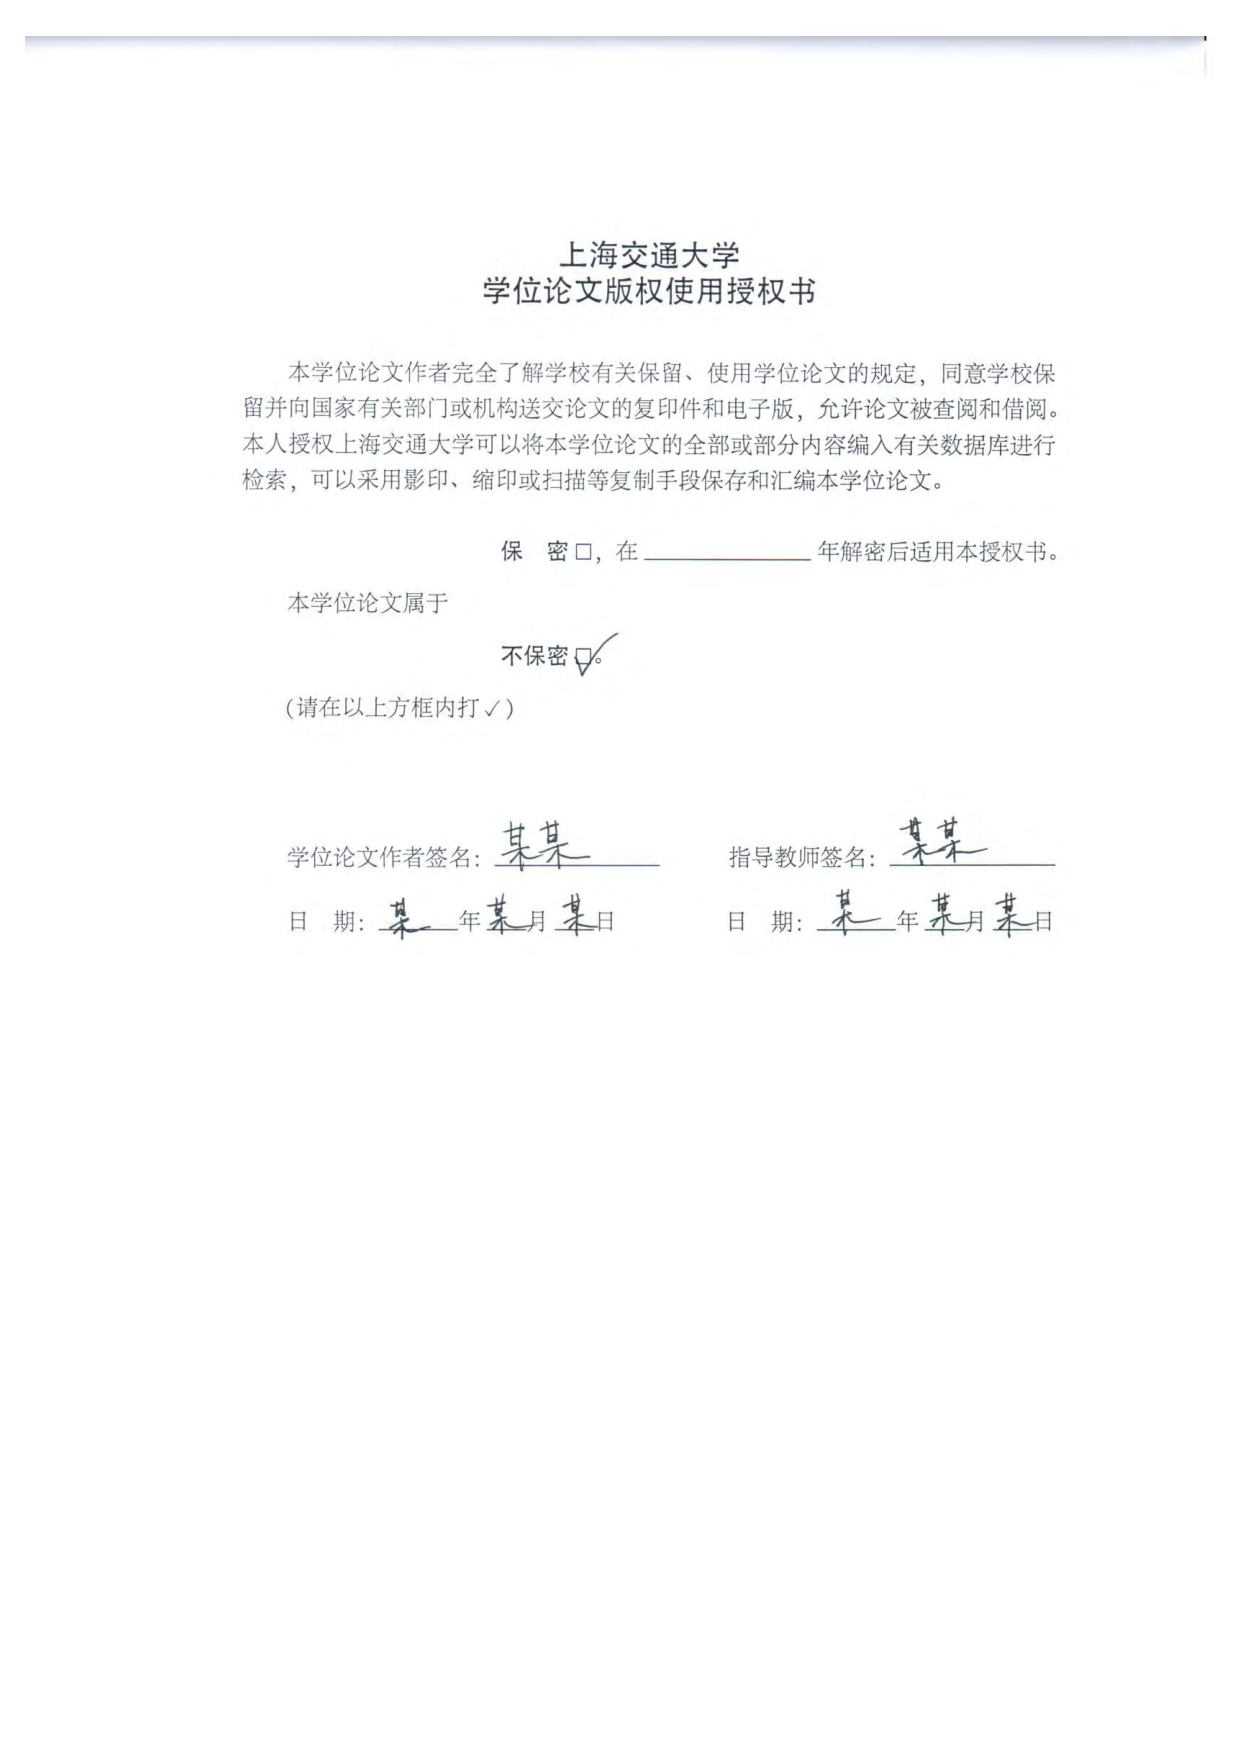
\includepdf{scans/authorization.pdf}
  \pdfbookmark[0]{\sjtu@label@authorization}{authorization}
  \cleardoublepage
\else
  \makeDeclareOriginality
  \makeDeclareAuthorization
\fi
\makeatother

%---------------------------------------------------------------------
\frontmatter

%%
%% Copyright (c) 2018 Weitian LI <liweitianux@sjtu.edu.cn>
%% Creative Commons BY 4.0
%%

% 中文摘要,约 3000 字
\begin{abstract}
\acl*{rh}如何影响 EoR 探测...
\end{abstract}

%---------------------------------------------------------------------

\begin{englishabstract}
\acs*{rh} can impose serious contamination on the EoR detection ...
\end{englishabstract}


\tableofcontents
\listoffigures
\listoftables

\acsetup{list-style=longtable}
\printacronyms[
  include-classes=symbol,
  name={主要符号对照表},
]

%---------------------------------------------------------------------
\mainmatter
\pagestyle{main}

%%
%% Copyright (c) 2018-2019 Weitian LI <liweitianux@sjtu.edu.cn>
%% Creative Commons BY 4.0
%%

\chapter{绪论}
\label{chap:introduction}

%=====================================================================
\section{研究背景和意义}

理解宇宙的起源、结构和演化,是人类孜孜不倦追求的目标,相关探索在哲学和科学中均占据重要地位。
经过几十年的努力,宇宙学的\ac{bbt}终于成为标准模型
\cite{weinberg1972,weinberg2008,peebles1993,peacock1999}。
支持该理论的几个关键证据包括星系的红移--距离关系(即 Hubble 定律)、
\ac{cmb}辐射、星系的大尺度分布规律、早期元素丰度。

根据大爆炸宇宙学模型,宇宙起源于约 138 亿年前的一次大爆炸。
伴随着宇宙的膨胀,温度以及能量密度都逐渐降低,
宇宙依次经历了\ac{inflation}、\ac{bbn}、
\ac{recombination}、\ac{da}、\ac{reionization}、
形成星系及大尺度结构等阶段(\autoref{fig:univ-history})。

\begin{figure}[htp]
  \centering
  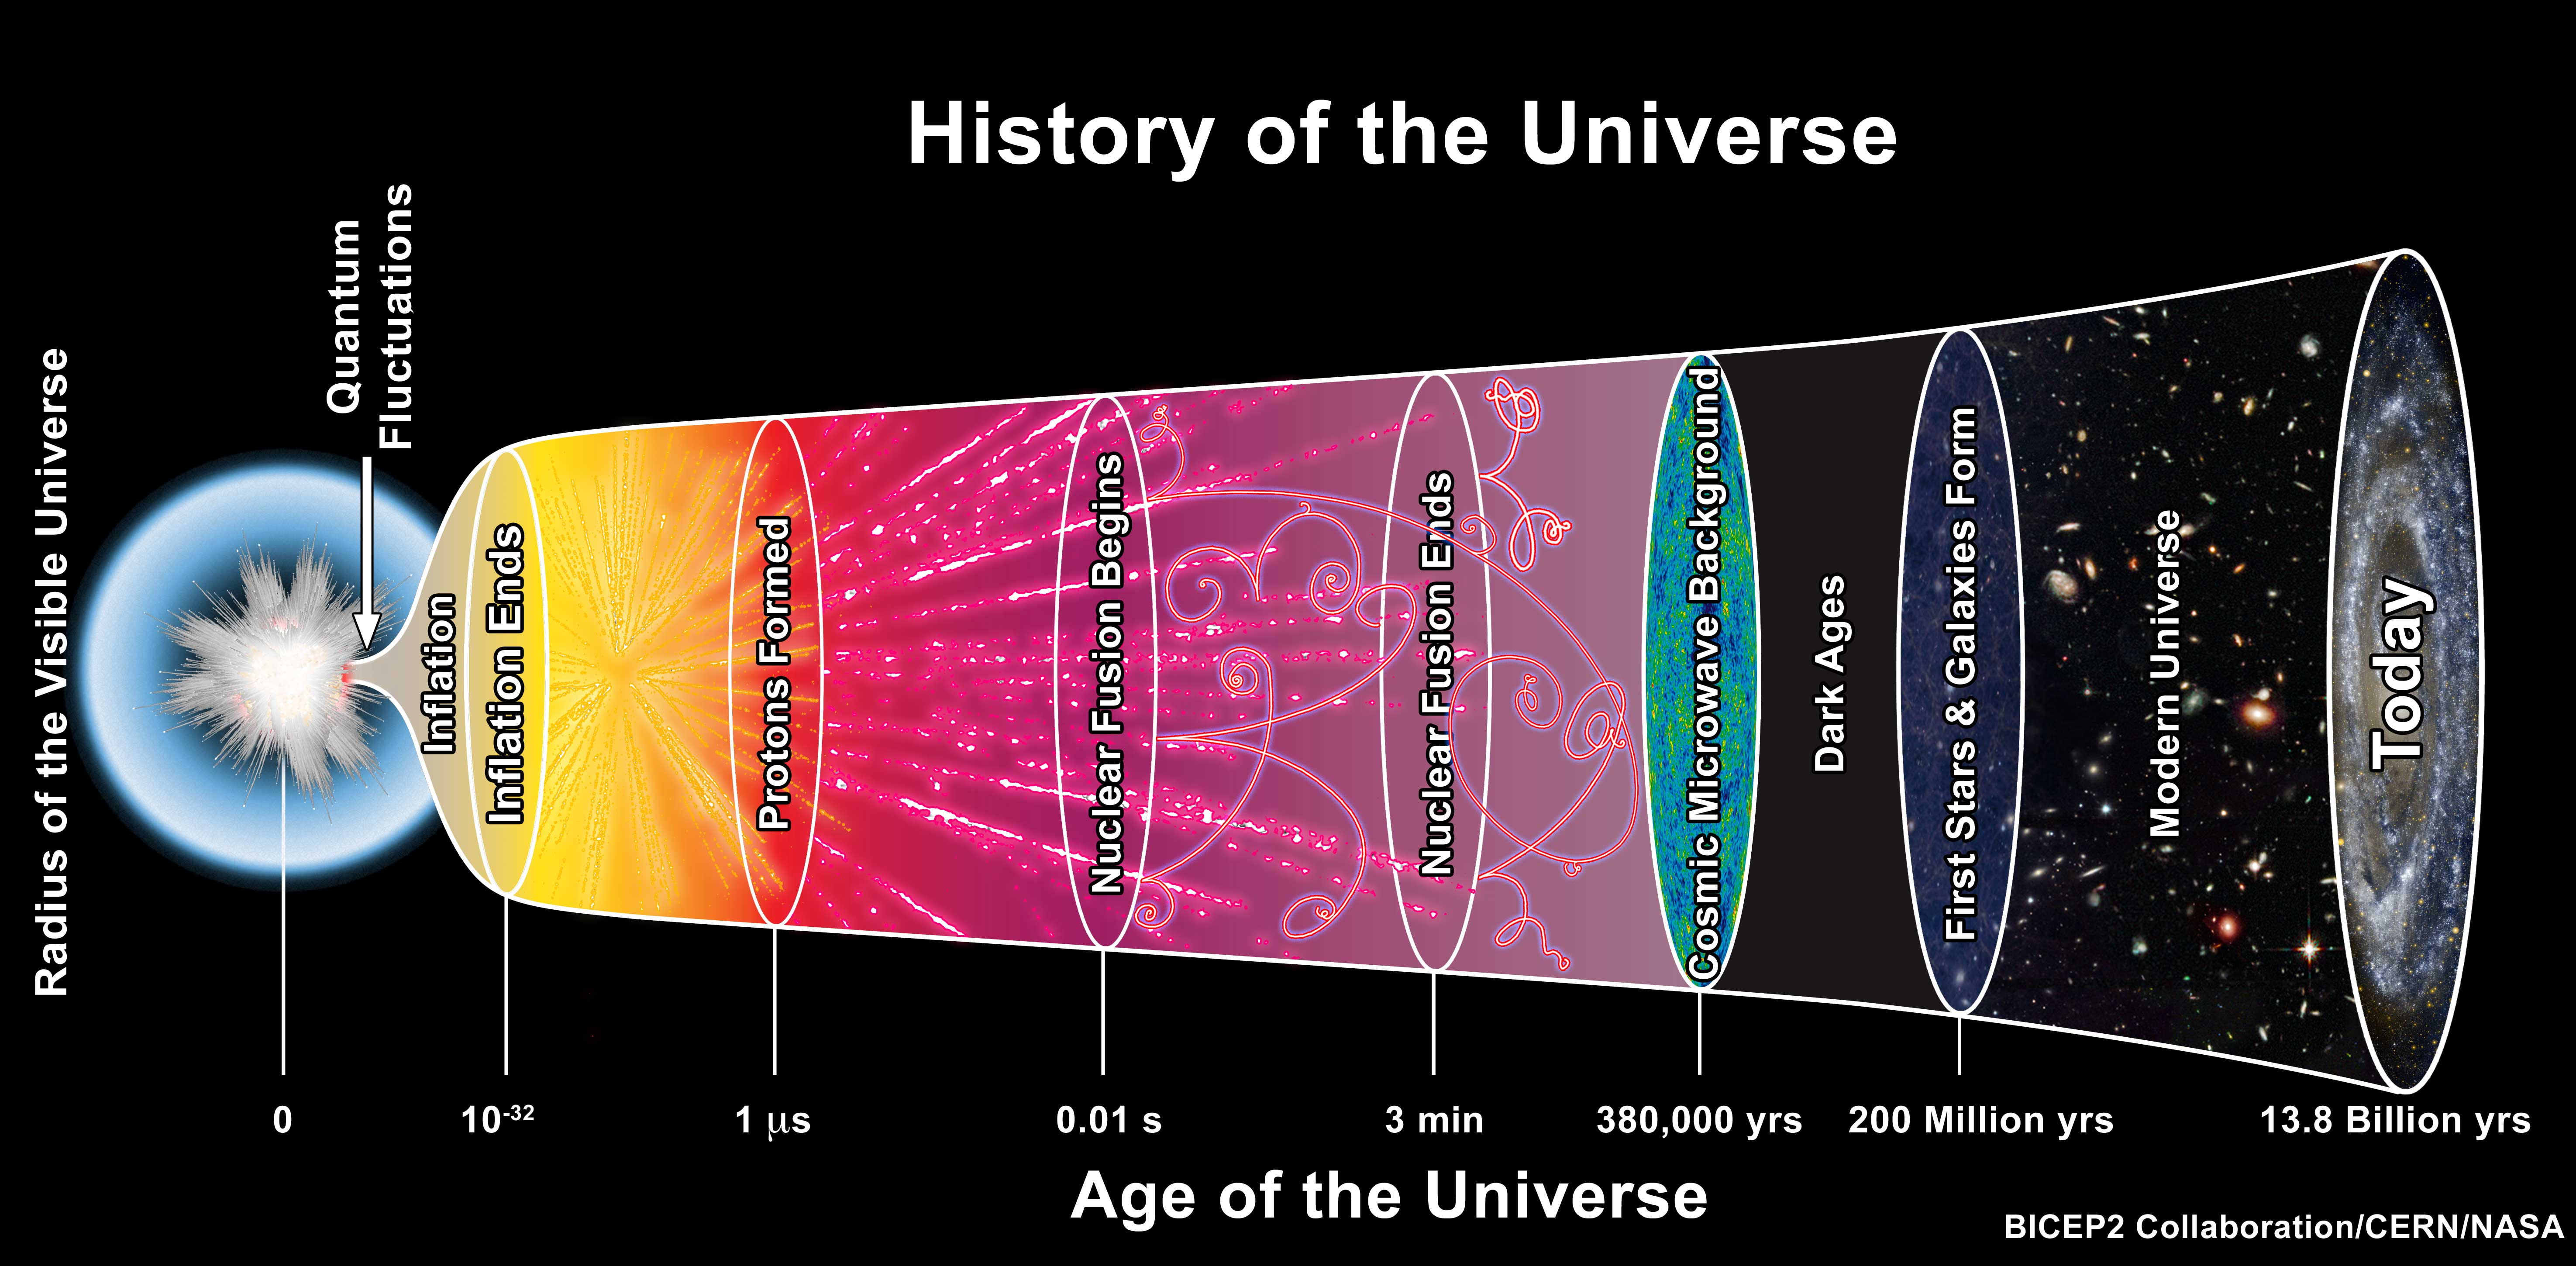
\includegraphics[width=\textwidth]{universe-history}
  \bicaption{%
    宇宙从大爆炸到今天的演化历史
  }{%
    The evolution of the Universe from the Big Bang
    to the present.
    \\来源/Credit:
    \ac{bicep}2/\ac{cern}/\ac{nasa}; \ac{cc}0 1.0
  }
  \label{fig:univ-history}
\end{figure}

大爆炸之后约 40 万年宇宙冷却至约 \SI{3000}{\kelvin},
自由电子遂与离子结合形成中性原子(即光子与重子物质脱耦),
光子得以在宇宙中自由传播。
此时及其之后的一段时期里,第一代天体尚未形成,因此宇宙进入了一个\ac{da}。
随着物质的密度扰动在引力作用下增长,第一代天体开始形成并产生辐射,
于是宇宙中的中性重子物质逐步被再次电离,宇宙从此结束了\ac{da}并进入\ac{eor}。
随着各尺度上的天体结构的逐步形成与演化,重子物质被充分电离,形成了今天的格局
\cite{peebles1980,peebles1993,peacock1999}。

通过研究 \ac{cmb},我们对宇宙的极早期历史
($\ac{redshift} \gtrsim 1100$,即自由电子\ac{recombination}之前)有了深刻理解。
另一方面,我们已借助多波段观测掌握了大量有关宇宙近期
($\ac{redshift} \lesssim 6$,即宇宙已充分电离之后)的演化信息。
然而,我们对中间那段 $\ac{redshift} \sim \numrange{6}{1100}$ 的时期却知之甚少。
其中距离相对较近 $\ac{redshift} \sim \numrange{6}{15}$ 的时期称为 EoR,
从宇宙大爆炸之后约 \SI{300}{\Myr} 一直延续到约 \SI{1}{\Gyr}。
在这个时期,第一代恒星和星系刚形成不久,
其紫外和软 X 射线辐射使中性重子物质逐渐被再次电离。
针对 EoR 的探测,目前仅能获得非常有限的间接观测信息,
例如,该时期的\ac{hi}对高红移\ac{quasar}的 Lyα 吸收 \cite{becker2001},
自由电子对 \ac{cmb} 光子的 Thomson 散射 \cite{kaplinghat2003},等。
但是有关 EoR 的一些关键问题仍然很不清楚,这些问题包括:
第一代天体是何时以及如何形成的?
主要的电离源有哪些?它们对再电离过程的贡献分别如何?
\ac{hii}区的尺度以及演化过程如何?
可见,EoR 的研究对于理解宇宙早期结构和星系的形成及其演化具有重要意义,
是建立完整的宇宙演化图景的关键之一。
详见 \citeay{fan2006}, \citeay{morales2010},
\citeay{pritchard2012}, \citeay{zaroubi2013},
\citeay{koopmans2015}, \citeay{mcQuinn2016} 等综述文。

尽管 EoR 阶段缺乏发光天体可供观测,
但是宇宙中丰富的\ac{hi}所辐射的 \ac{21cmline}(详见 \autoref{sec:eor-signal})
为直接探测 EoR 提供了一条可能途径。
事实上,对 21\,cm 信号的探测是目前对 EoR 开展系统性研究的最直接而有效的观测手段
\cite{madau1997,tozzi2000,furlanetto2006,koopmans2015,furlanetto2016}。
\ac{hi} \ac{21cmline}的本征频率约为 \SI{1420}{\MHz};
理论预测源自 EoR 的 \ac{21cmline}经历显著红移后应出现在约
\SIrange{90}{200}{\MHz} 之间,对应于低频射电波段。
EoR 信号到达地球时已非常微弱,亮温度仅约几 \si{\mK} 至十几 \si{\mK},
需要具有极高灵敏度的低频观测设备才能开展观测。
目前已建成或正在建设的低频射电干涉阵列主要包括:
\ac{21cma} \cite{zheng2016}、
\ac{gmrt} \cite{paciga2011}、
\ac{mwa} \cite{bowman2013,tingay2013}、
\ac{lofar} \cite{vanHaarlem2013}、
\ac{lwa} \cite{ellingson2009}、
\ac{paper} \cite{parsons2010}、
\ac{hera} \cite{deBoer2017}、
\ac{ska} \cite{mellema2013,koopmans2015}。
必须指出的是,利用干涉阵列探测 EoR 信号面临诸多困难与挑战
\cite{morales2010,wijnholds2010},
例如,如何识别并扣除强烈的前景干扰,如何扣除人工源的\ac{rfi},如何修正电离层的扰动,
如何有效地校准仪器,如何存储并处理海量数据,如何进行高动态范围成像
(详见 \autoref{sec:det-difficulties})。

在低频射电波段,强烈的前景干扰(主要源自银河系以及河外点源;
\autoref{sec:fg-intro})比待探测的 EoR 信号高出约 5 个数量级,
即使是其涨落也达待测 EoR 信号强度的数千倍 \cite{zaroubi2013}。
从这个意义上讲,准确把握前景干扰并将其扣除是成功探测 EoR 信号的关键。
目前,低频射电波段的观测仍然十分有限,巡天数据严重不足
\cite{deOliveiraCosta2008,zheng2017gal},
导致我们对 EoR 前景的理解程度远远不够
\cite{liu2012,harker2015,offringa2016,murray2017,procopio2017}。
因此,需要挖掘已有中高频射电以及其他波段的海量观测数据,同时结合逐渐积累的低频观测数据,
深入理解 EoR 探测中的低频射电前景并为其构建完善模型,
为识别和提取 EoR 信号提供有力支撑。


%=====================================================================
\section{研究内容和目标}

本文的研究内容包括以下两大部分:
\begin{itemize}
\item \emph{射电晕辐射建模的改进以及对 EoR 探测影响的评估}

\hspace{2\ccwd}%
深刻理解各前景成分的性质(如强度、空间分布、频谱结构)并充分把握它们对 EoR 探测的干扰方式,
是研发具有针对性的\ac{fg-rm}和 EoR 信号分离算法的前提与关键。
在现阶段缺乏足够可用的高质量低频观测数据的情况下,
借助于挖掘已有多波段观测数据来准确模拟低频射电天空,
是开展前景干扰研究以及 EoR 信号分离算法研发的可行办法。

\hspace{2\ccwd}%
在各前景成分之中,银河系的弥散辐射 [包括\ac{rad-syn}和\ac{rad-ff}]
以及河外\ac{src-point}辐射是最主要的成分,已被比较广泛地研究
\cite{shaver1999,diMatteo2004,gleser2008,liu2012,murray2017,spinelli2018}。
在剩下的前景辐射之中,来自河外射电\ac{src-extended}的辐射占据主导地位,
主要包括\ac{icm} \cite{feretti2012} 产生的\ac{rh}、\ac{rr}和\ac{rmh},
\ac{gc}外围区域的\ac{igm} \cite{keshet2004}。
这些河外射电\ac{src-extended}的低频射电观测证据并不多,
尚不明确它们将如何影响 EoR 探测。

\hspace{2\ccwd}%
与其他几类河外射电\ac{src-extended}相比,星系团\ac{rh}拥有更多的观测数据和理论研究,
使我们有可能构建一个更完善、更物理的模型用来模拟其低频射电辐射特征,
从而改进低频射电天空的模拟,在更加逼真的条件下定量评估不同 EoR 信号探测方法的优劣。

%.......................................
\item \emph{研发 EoR 信号分离算法}

\hspace{2\ccwd}%
目前已提出一系列方法用来提取淹没于前景干扰之中的 EoR 信号,
这些前景处理方法可大致分为\ac{fg-rm}和\ac{fg-avd}两大类 \cite{chapman2016}
(详见 \autoref{sec:fg-methods})。
前者依赖于一个重要前提:前景辐射的频谱必须非常光滑,可通过构建一个模型来合理地描述。
后者则假定前景干扰被有效地约束在二维功率谱的一个区域内,
于是可以通过尽量避开前景污染区域达到提取 EoR 信号的目标。

\hspace{2\ccwd}%
然而在实际情况中,干涉阵列的\ac{beam}存在频率依赖效应(以下简称波束效应),
即\ac{beam}的形状会随观测频率而变化,导致原本光滑的前景频谱产生快速变化的起伏,
使前景频谱的光滑性遭到损坏 \cite{liu2009ps},
因此现有\ac{fg-rm}方法难以区分前景干扰与 EoR 信号,
从而无法正确地分离 EoR 信号(详见 \autoref{sec:beam-effect})。

\hspace{2\ccwd}%
考虑到干涉阵列\ac{beam}形状非常复杂,为传统前景处理方法打造一个实际可用的模型
用以克服波束效应非常困难 \cite{lochner2015}。
\ac{dl}方法能够从数据中学习特征并自适应地优化模型,
因此基于\ac{dl}的 EoR 信号分离算法能够学习干涉阵列的波束特征,
将是一条可能的解决问题的途径 \cite{herbel2018,vafaeiSadr2019}。

\end{itemize}

综合上述讨论,我们为本工作设定了如下研究目标:
(1)改进\ac{rh}的模拟,在考虑干涉阵列仪器效应的前提下获得更精细、
更符合实际的低频射电天空的模拟图像,评估\ac{rh}辐射对 EoR 信号探测的影响;
(2)基于\ac{dl}研发能够有效克服干涉阵列波束效应的 EoR 信号分离新算法,
并运用到上述模拟数据进行测试和优化。


%=====================================================================
\section{研究方案}

本文遵循以下主要步骤开展工作,完成研究内容,达到研究目标:
\begin{enumerate}
\item
调研\ac{rh}的相关理论研究和观测证据,理解其形成机制和演化规律,
构建模型并模拟\ac{rh}在低频射电波段的\ac{skymap}。
搜集\ac{rh}的现有观测数据,约束模型参数,获得可靠的模拟结果。

\item
采用 SKA1-Low 干涉阵列的布局方案,
从上一步所得的\ac{skymap}模拟得到\ac{vis}数据,
然后成像获得高仿真 SKA1-Low 图像。
通过这种模拟,干涉阵列的复杂仪器效应(如波束效应)可有效地整合到数据分析流程之中。

\item
基于上述模拟所得的 SKA1-Low 图像,利用一维和二维\ac{ps}对比\ac{rh}和 EoR 信号,
量化\ac{rh}辐射在运用\ac{fg-rm}法或\ac{fg-avd}法的情况下对 EoR 信号探测的影响,
评估并研究\ac{rh}干扰的重要性。

\item
从目前主流的\ac{dl}算法中筛选出适用于 EoR 信号分离的算法并加以必要的改善,
利用上述模拟数据对算法进行训练和调优,研究新算法的可行性和优势。

\end{enumerate}


%=====================================================================
\section{本文框架}

本文余下章节安排如下:
\autoref{chap:radio-astronomy}将介绍射电天文学和射电干涉技术的基础知识,
主要包括基本辐射理论、天线原理、干涉成像技术等。
在\autoref{chap:detection},我们将介绍利用\ac{hi} 21\,cm 信号
探测 EoR 的主要方法、面临的困难、以及前景处理方法。
在\autoref{chap:simulation},我们首先模拟各前景成分和 EoR 信号的\ac{skymap},
然后进行干涉阵列的模拟观测,得到整合了实际仪器效应的\enquote{观测}图像。
据此,我们在\autoref{chap:halo}借助\ac{ps}量化评估\ac{rh}对
EoR 探测的具体影响。
\autoref{chap:cdae}将阐述我们提出的基于\ac{dl}的 EoR 分离新算法并演示其效果。
最后,我们对全文进行总结并作简要展望。

全文采用一个由 \lcdm 模型描述的平直宇宙,参数为:
$\acs{H0} = 100\,\acs{h}\,\si{\km\per\second\per\Mpc}
= \SI{71}{\km\per\second\per\Mpc}$,
$\acs{Om0} = 0.27$,
$\acs{Ol0} = 1 - \acs{Om0} = 0.73$,
$\acs{Ob0} = 0.046$,
$\acs{ns} = 0.96$ 以及 $\acs{sigma8} = 0.81$。
如无额外说明,本文给出的误差对应 68\% 的置信水平;
使用的幂律谱形式为 $\acs{S-nu} \propto \acs{freq}^{-\acs{spec-index}}$,
其中 \acs{S-nu} 为\acl{S-nu}, \acs{spec-index} 为\acl{spec-index}。
本文使用的中文术语遵循\href{%
  http://astrodict.china-vo.org/
}{英汉天文学名词数据库}\footnote{%
  英汉天文学名词数据库:
  \url{http://astrodict.china-vo.org/}}
以及 Google 的\href{%
  https://developers.google.com/machine-learning/glossary/?hl=zh-CN
}{机器学习术语表}\footnote{%
  机器学习术语表:
  \url{https://developers.google.com/machine-learning/glossary/?hl=zh-CN}}。


%% EOF

%%
%% Copyright (c) 2018-2019 Weitian LI <liweitianux@sjtu.edu.cn>
%% Creative Commons BY 4.0
%%

\acuse{freq,wavelength}

\chapter{射电天文学基础}
\label{chap:radio-astronomy}

%=====================================================================
\section{射电天文学简介}
\label{sec:radio-astro-intro}

%---------------------------------------------------------------------
\subsection{简介和历史}

我们对宇宙的几乎所有认识都来自于观测并研究所接收到的电磁辐射。
在射电波段对天体和宇宙开展研究的天文学分支称为射电天文学。
对于地面上的射电望远镜,观测频率的下限约为 $\nu_{\R{min}} \sim \SI{10}{\MHz}$
(即最长波长 $\lambda_{\R{max}} \sim \SI{30}{\meter}$),
取决于\ac{ionosphere}的截断频率,
低于该频率的电磁波将被\ac{ionosphere}反射而无法到达地面。
观测频率的上限约为 $\nu_{\R{max}} \sim \SI{1000}{\GHz}$
(即最短波长 $\lambda_{\R{min}} \sim \SI{0.3}{\mm}$),
更高频率的电磁波将被\ac{troposphere}中的分子
(主要是 $\mathrm{H_2 O}$ 和 $\mathrm{O_2}$)吸收。
大气层对电磁辐射的吸收情况还会随时间以及地理位置而变化。
\autoref{fig:atmospheric-emt} 显示了大气层的
电磁辐射\ac{transmittance}随波长的变化情况以及射电观测窗口。

\begin{figure}[htp]
  \centering
  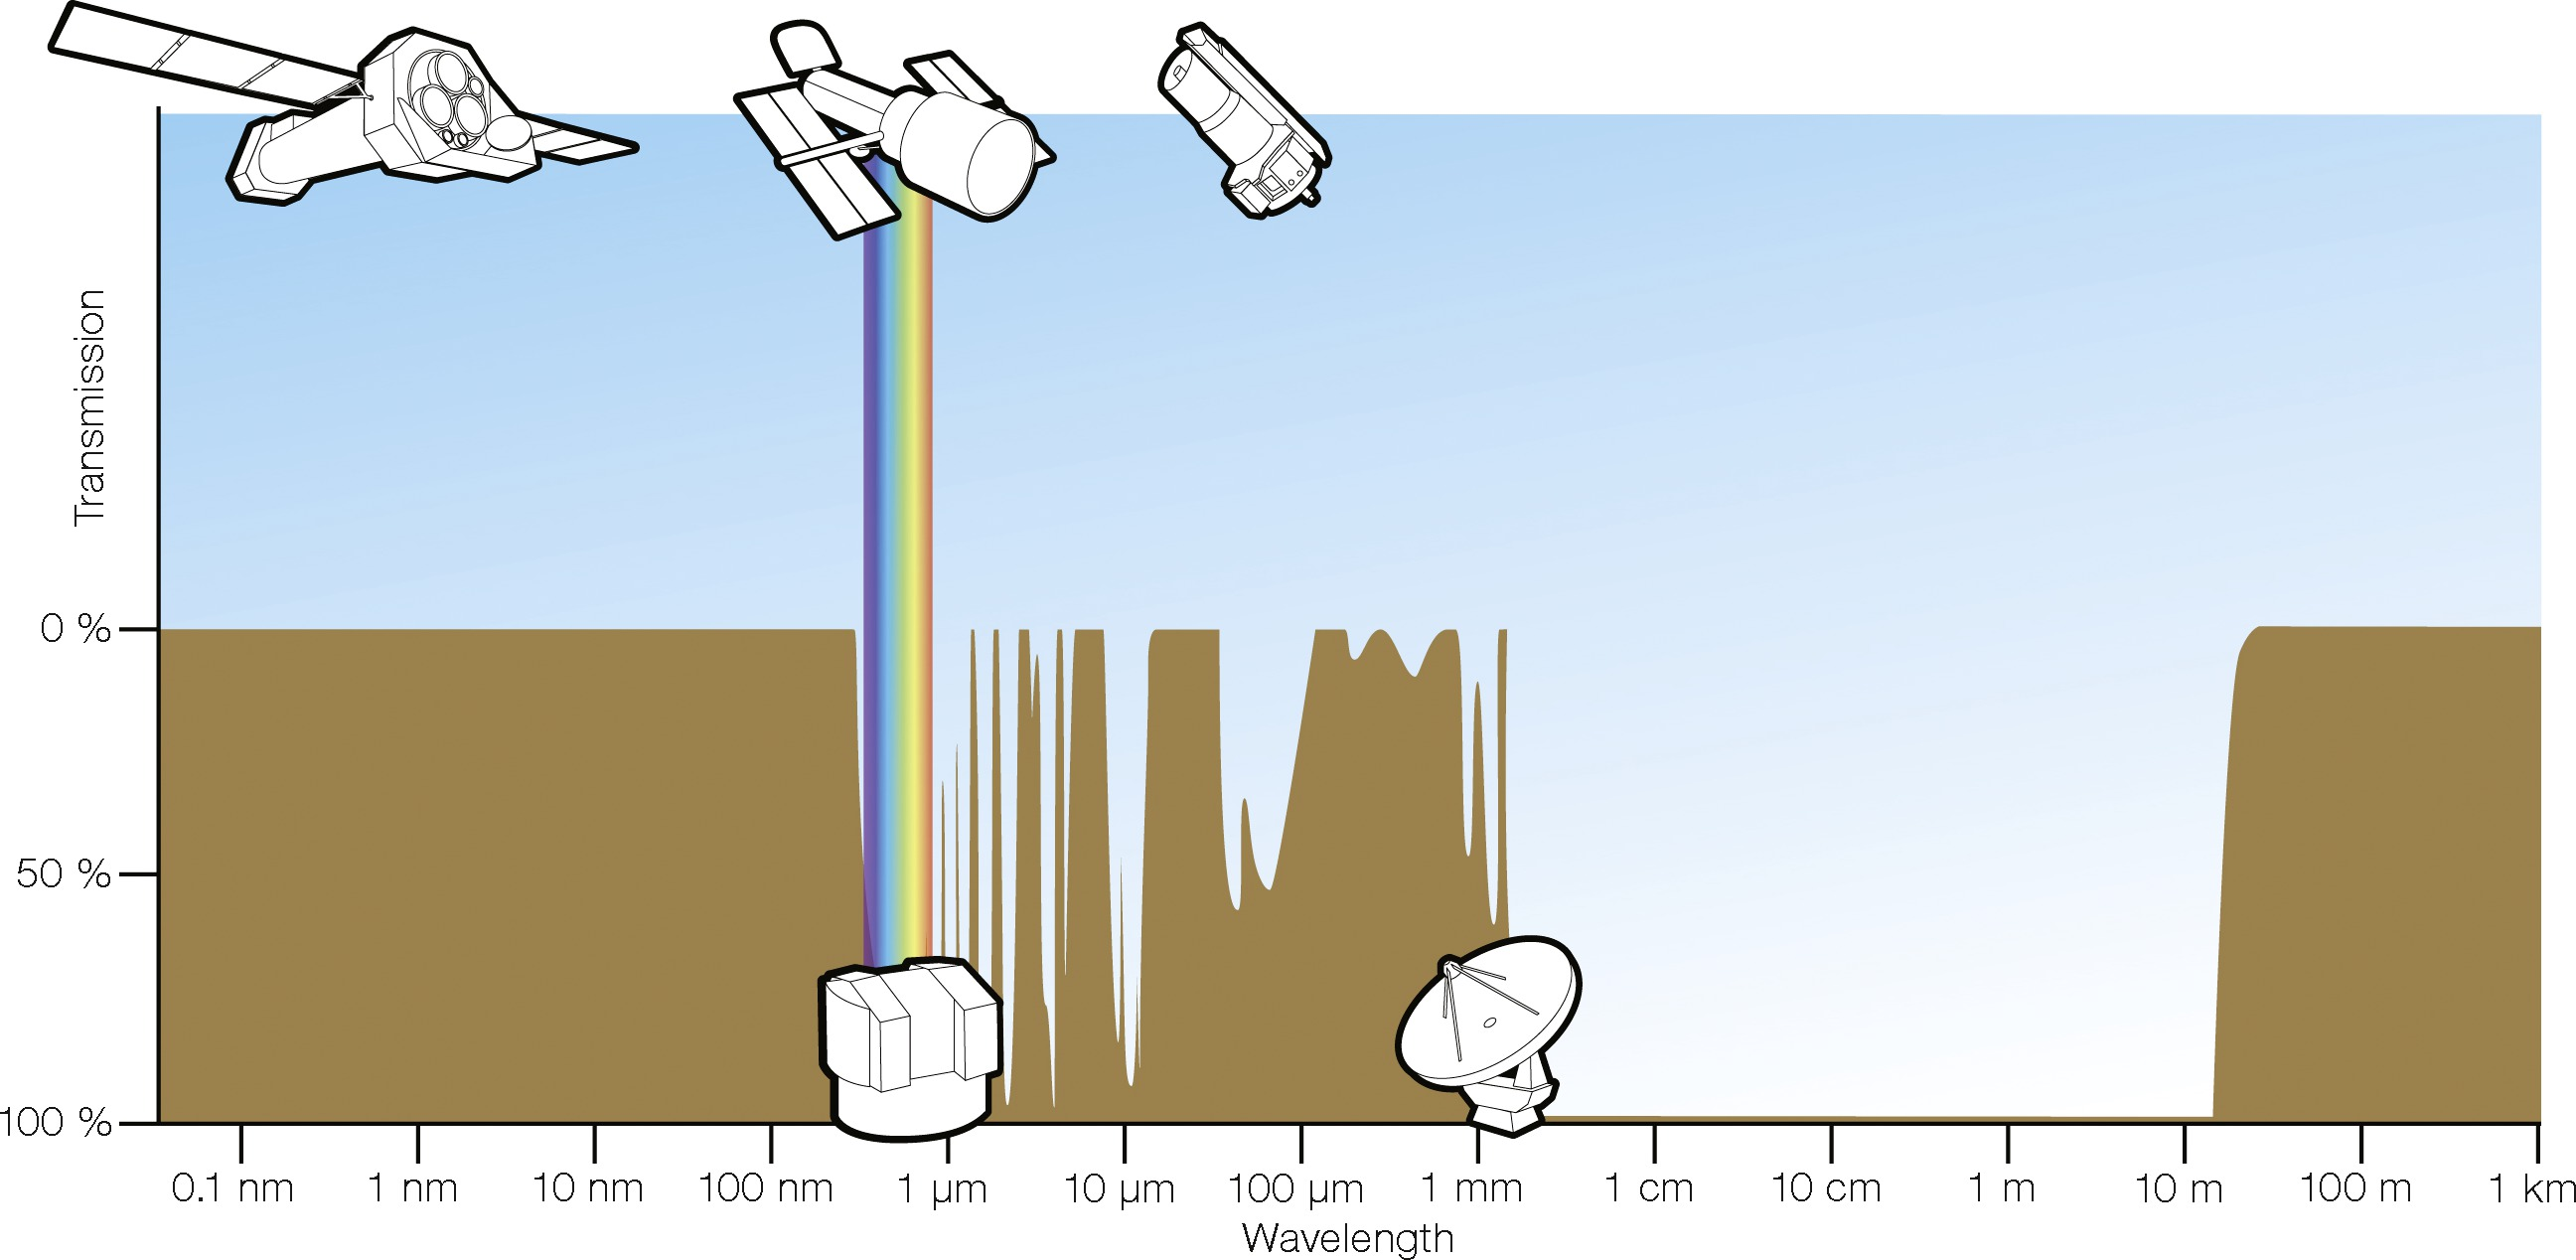
\includegraphics[width=\textwidth]{atmospheric-em-transmittance}
  \bicaption[大气层的电磁辐射透射率随波长的变化]{%
    大气层的电磁辐射\acs*{transmittance}随波长 $\lambda$(即频率 $\nu$)的变化。
    除了光学窗口,大气层还有一个更宽的射电窗口,
    从 $\lambda \sim \SI{0.3}{\mm}$ ($\nu \sim \SI{1000}{\GHz}$)
    延伸到 $\lambda \sim \SI{30}{\meter}$ ($\nu \sim \SI{10}{\MHz}$)。
  }{%
    Electromagnetic transmittance of the Earth's atmosphere.
    In addition to the visible optical window, there is another
    much wider radio window, which spans from
    $\lambda \sim \SI{0.3}{\mm}$ ($\nu \sim \SI{1000}{\GHz}$)
    to $\lambda \sim \SI{30}{\meter}$ ($\nu \sim \SI{10}{\MHz}$).
    \\来源/Credit:
    \citeay{condon2016}, \S\,1.1.2
  }
  \label{fig:atmospheric-emt}
\end{figure}

首次发现源自地球之外的射电辐射是在 1932 年被 Bell 电话实验室的工程师
Karl G. Jansky 意外得到的。
上世纪 20 年代,Bell 电话公司基于 $\lambda \sim \SI{15}{\meter}$
的短波传输建设了跨洋电话服务,但是发现通话受到了强烈的干扰,因此派 Jansky 去查明干扰来源。
Jansky 建造了一个对方向敏感的可转动天线(如\autoref{fig:jansky-antenna} 所示)
用来监测 \SI{20.5}{\MHz} ($\lambda \approx \SI{14.6}{\meter}$) 处的射电辐射。
经过观测,他发现绝大部分的干扰源自暴风雨的闪电。
此外,他还发现有一个较弱的不明噪声,其强度在每天发生周期性的变化。
因此 Jansky 怀疑该噪声可能是太阳的射电辐射。
但是持续的观测显示这个不明噪声的准确周期为 \SI{23}{\hour}\,\SI{56}{\minute},
并不是恰好 \SI{24}{\hour}。
将此困惑与他的一个天文学家朋友 Albert M. Skellett 讨论后,
Jansky 了解到该噪声来自太阳系之外,并进一步确认其来源是银河系中心 \cite{jansky1933}。

\begin{figure}[htp]
  \centering
  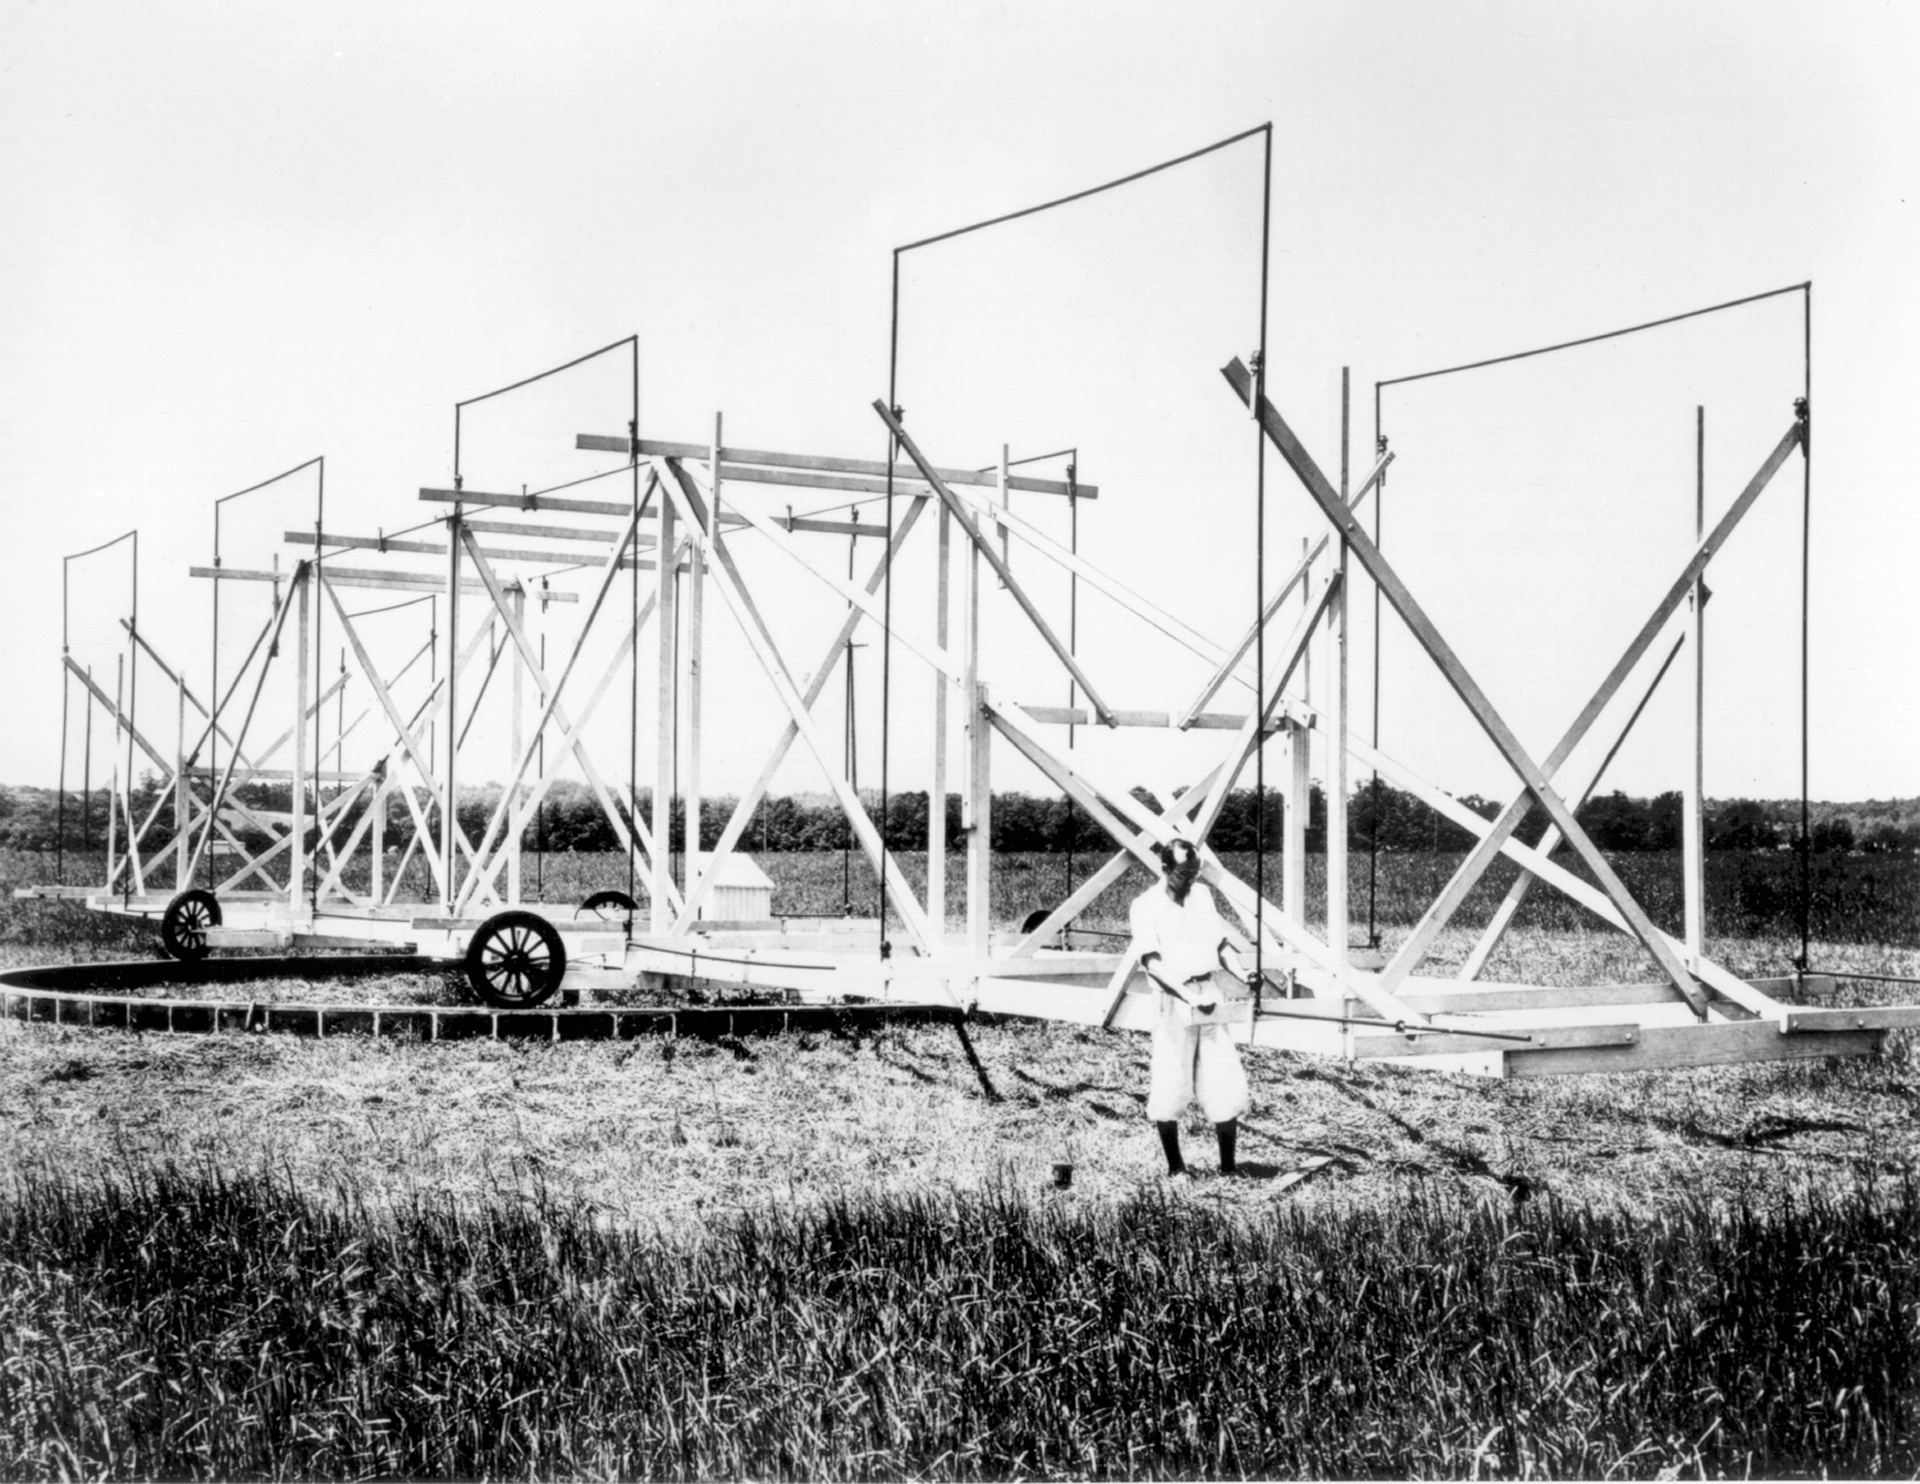
\includegraphics[width=0.8\textwidth]{KarlJansky-antenna}
  \bicaption[Karl G. Jansky 和他的天线]{%
    Karl G. Jansky 和帮助他发现银河系射电辐射的天线。
    该天线可转动,主要接收水平方向的辐射。
  }{%
    Karl G. Jansky and the antenna that discovered the
    Galactic radio emission.
    The antenna can rotate in azimuth and mainly receive horizontal
    emissions.
    \\来源/Credit:
    \ac{nrao}/\ac{aui}/\ac{nsf}
  }
  \label{fig:jansky-antenna}
\end{figure}

然而 Jansky 的发现未能得到足够的关注和重视,
他本人也被分配到其他项目而无法继续研究银河系的射电辐射。
另一位无线电工程师 Grote Reber 恰好对 Jansky 的发现产生了极大兴趣,
于是耗时数年在自家后院建造了世界第一台抛物面射电望远镜
(\autoref{fig:reber-telescope}),
并在 1938 年成功地在 \SI{160}{\MHz} 探测到了银河系的射电辐射。
Reber 接着进一步开展了银河系的第一次射电巡天观测,并将结果发表于专业的天文学期刊
\textit{The Astrophysical Journal} \cite{reber1940}。
自此,射电天文学登上了天文学的舞台。

\begin{figure}[htp]
  \centering
  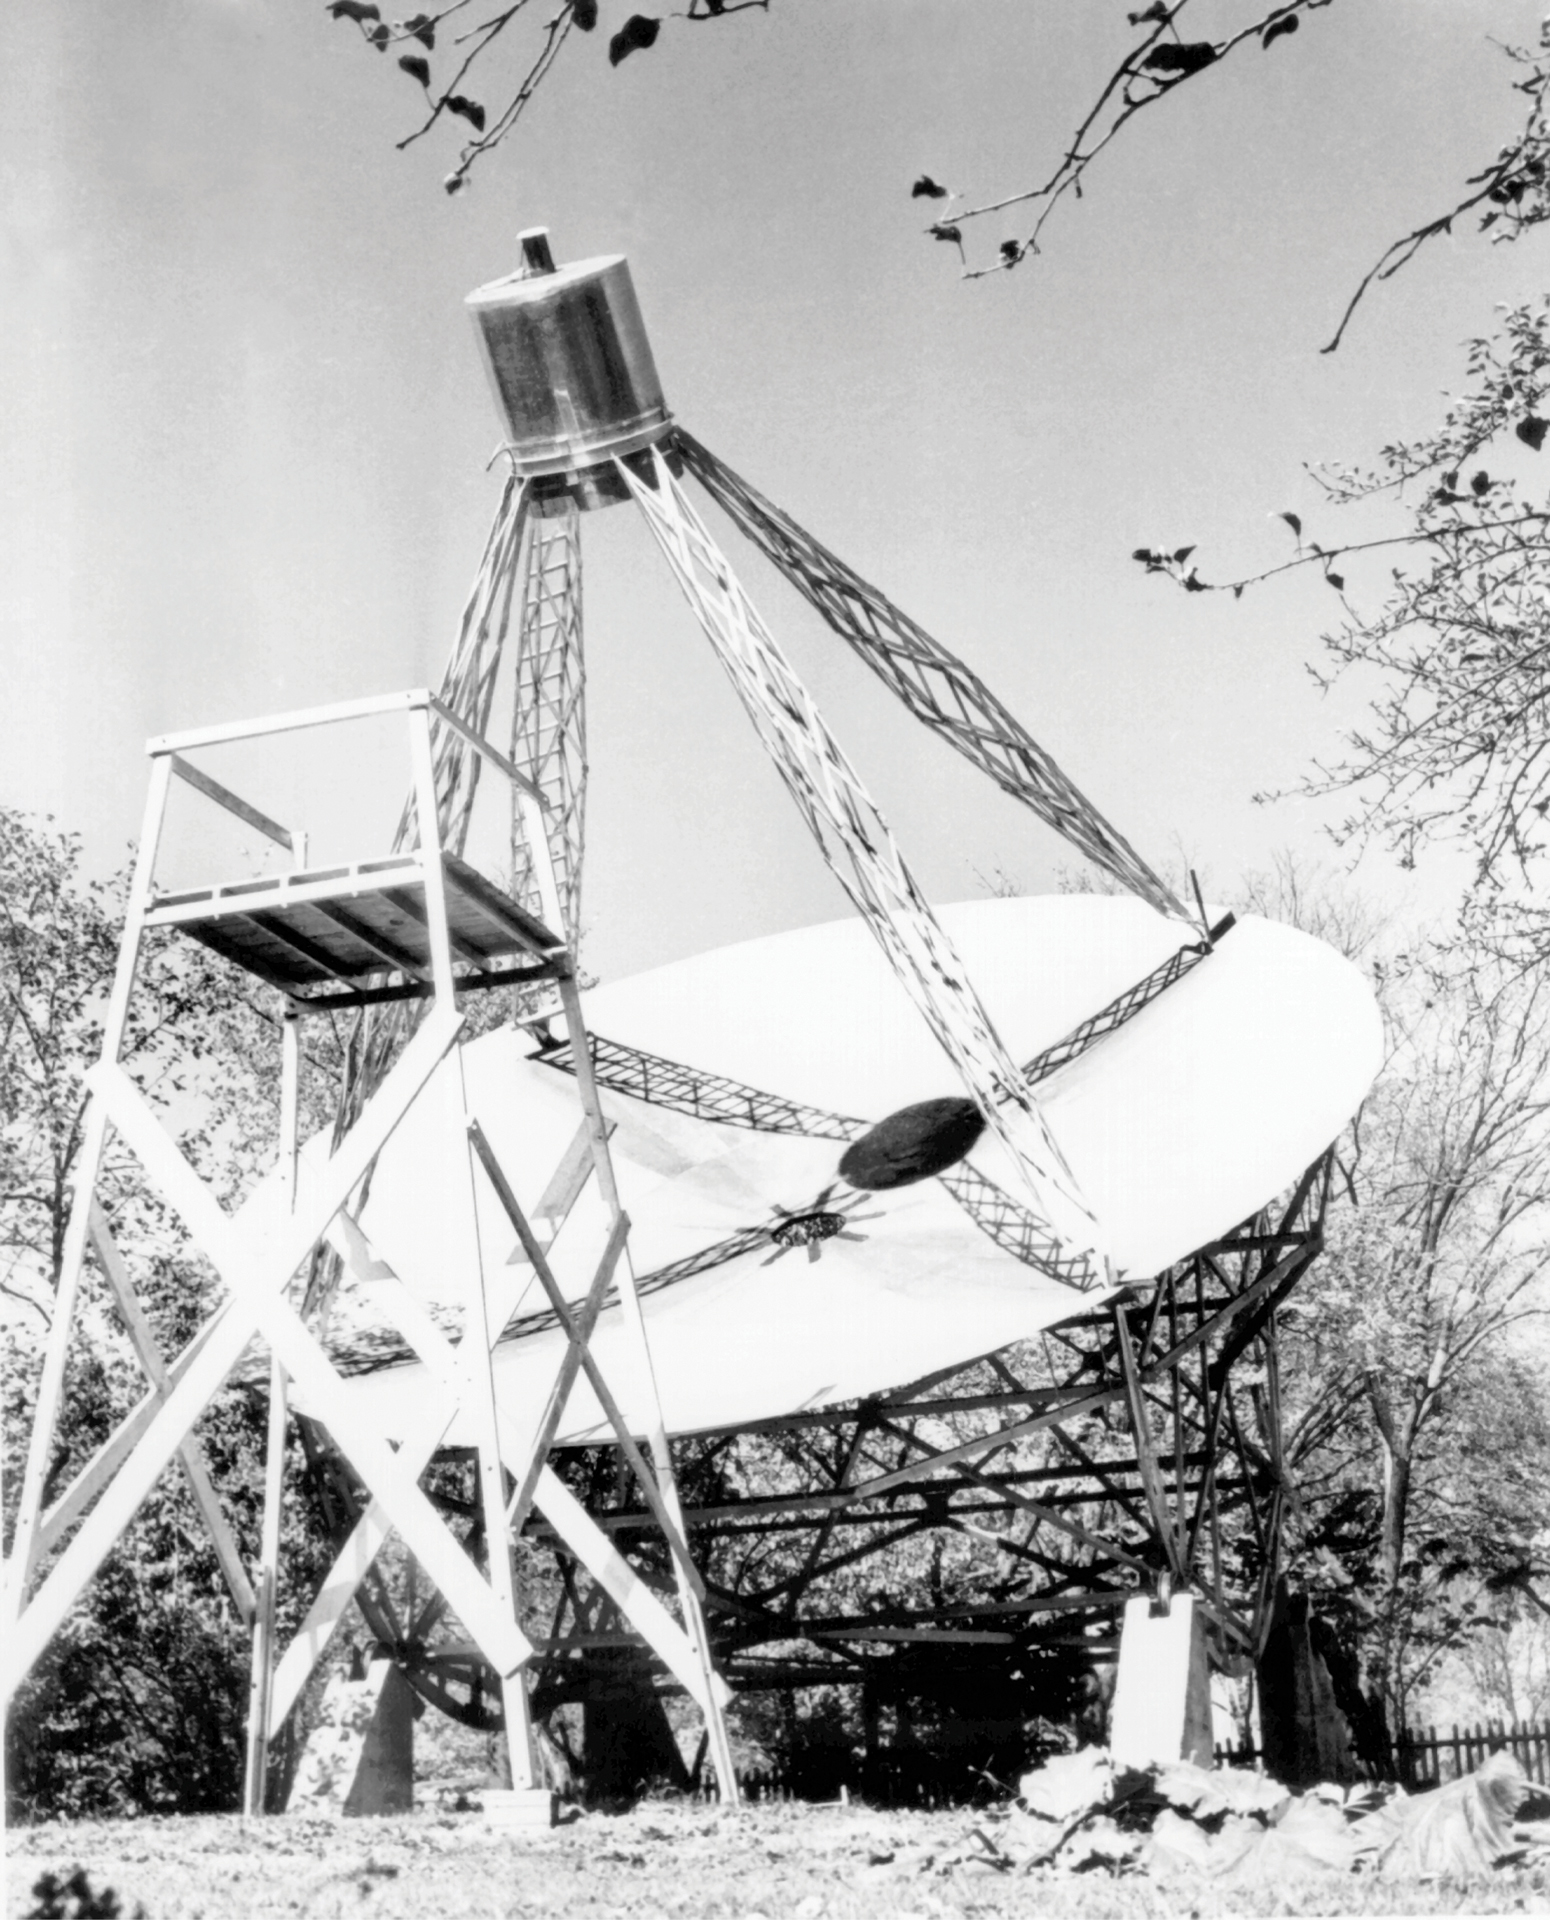
\includegraphics[width=0.6\textwidth]{GroteReber-telescope}
  \bicaption[Grote Reber 建造的抛物面射电望远镜]{%
    Grote Reber 在自家后院建造的射电望远镜,使用了直径约 \SI{10}{\meter} 的抛物面。
  }{%
    Grote Reber's backyard radio telescope using a parabolic reflector
    of diameter about \SI{10}{\meter}.
    \\来源/Credit:
    \acs{nrao}/\acs{aui}/\acs{nsf}
  }
  \label{fig:reber-telescope}
\end{figure}

在后续的几年里,尽管第二次世界大战阻碍了射电天文学的发展,
但是刺激了无线电技术和雷达设备的研发。
这些方面的成果在战争结束后给射电天文学带去了长足的进步,开创了一系列新技术和新方法。
其中最值得一提的是由 Martin Ryle 和 Antony Hewish 发明的\ac{as}技术 \cite{ryle1960},
使射电观测的角分辨率得到了空前的提高。

自射电窗口被打开以来,射电天文学已取得了一系列激动人心的发现,
其中代表性的发现包括:
银河系和其他多种天体的非热 (non-thermal) 辐射 \cite{reber1940}、
由超大质量黑洞驱动的射电星系\cite{baade1954}
和\ac{quasar}\cite{hazard1963,schmidt1963}、
冷\ac{ism}的热辐射谱线、
星际分子的\ac{maser} \cite{weaver1965}、
宇宙大爆炸的 \ac{cmb} \cite{penzias1965}、
\ac{pulsar}和中子星 \cite{hewish1968}、
星系中的\ac{dm} \cite{roberts1975}、
\ac{gl-strong} \cite{walsh1979}。
总之,射电天文学揭开了宇宙的全新一面(如\autoref{fig:radio-sky} 所示),
拓展了我们对宇宙的认识,深刻地改变了我们对宇宙的理解。

\begin{figure}[htp]
  \centering
  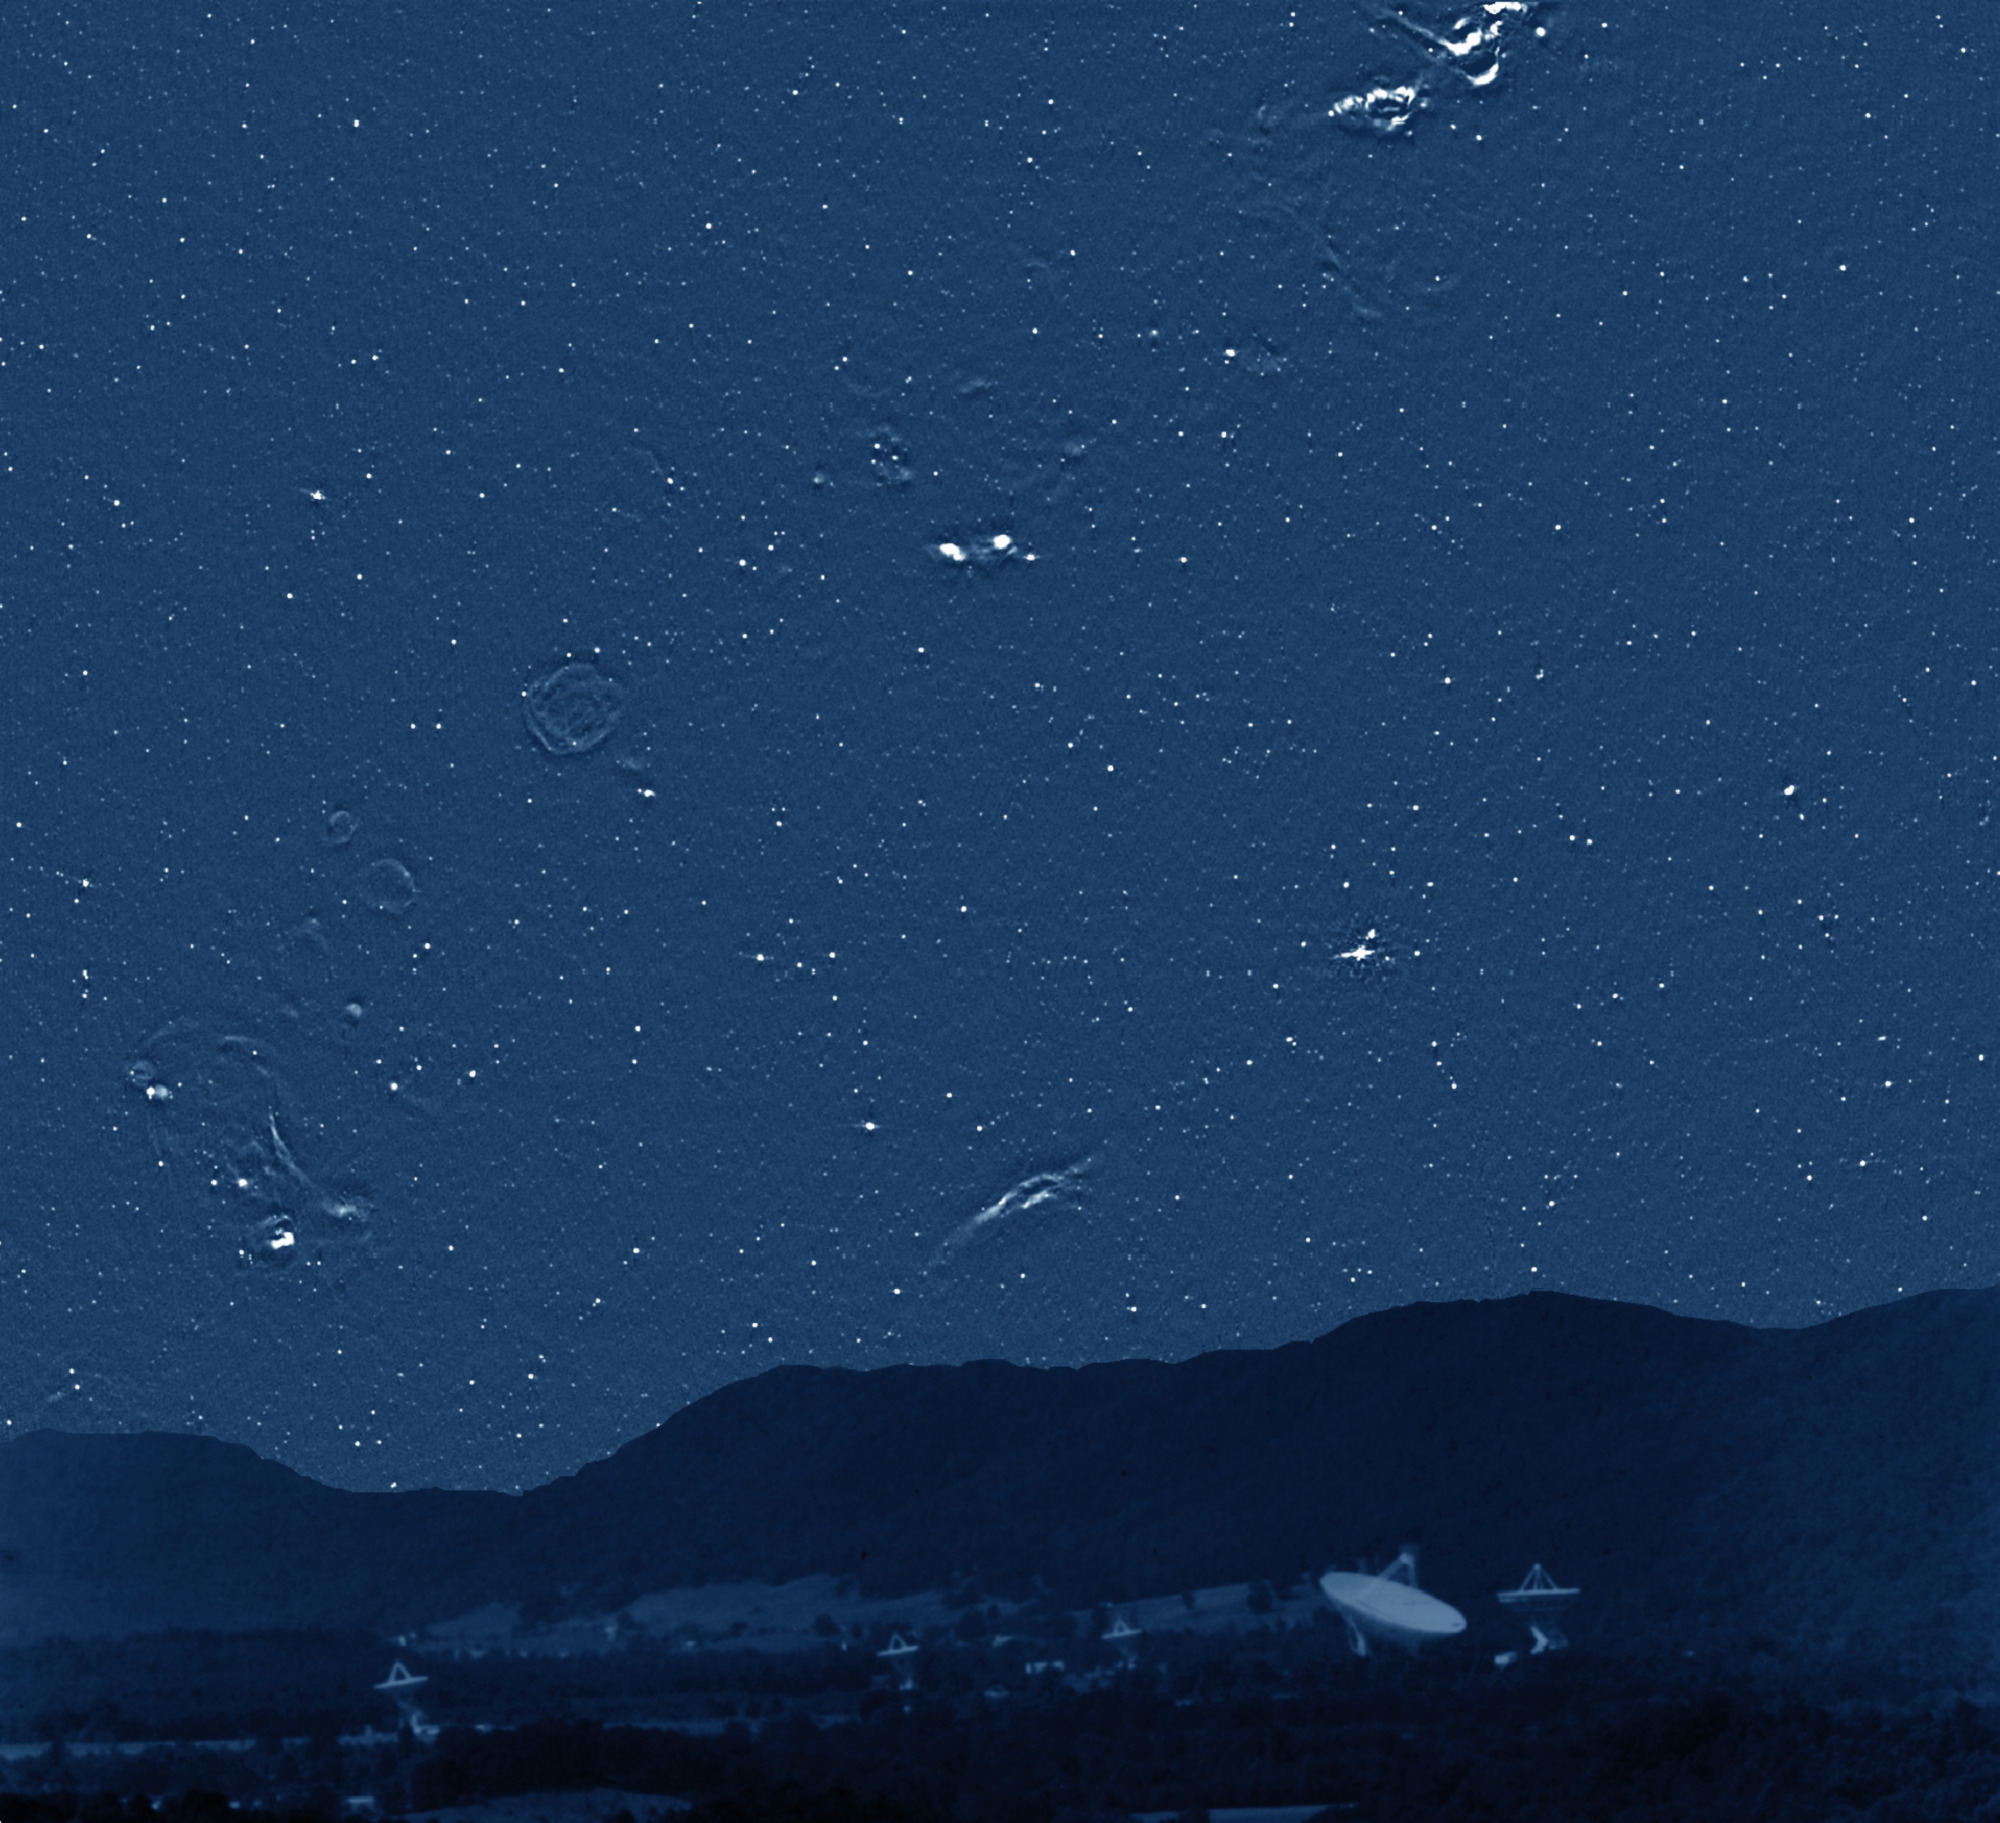
\includegraphics[width=0.8\textwidth]{nrao-radio-sky}
  \bicaption[与光学波段所见完全不同的射电天空]{%
    在 NRAO 台址的照片上方显示了由 NRAO 昔日的 \SI{91}{\meter} 射电望远镜
    获得的 \SI{4.85}{\GHz} 射电天空图像,展示了与光学波段所见完全不同的景象。
  }{%
    The \SI{4.85}{\GHz} radio sky made with the NRAO former \SI{91}{\meter}
    telescope is shown above an old photograph of the NRAO site,
    showing a very different scene from seeing in the optical band.
    \\来源/Credit:
    \acs{nrao}/\acs{aui}/\acs{nsf}
  }
  \label{fig:radio-sky}
\end{figure}

%---------------------------------------------------------------------
\subsection{低频波段的机遇和挑战}

尽管大气层的射电窗口允许低至 $\sim$\,\SI{10}{\MHz} 的观测,但由于各种技术和条件的限制,
以往的射电观测和研究主要在 $\gtrsim$\,\SI{1}{\GHz} 的中高频波段。
相比中高频波段,低频波段主要拥有以下几个优势:
\begin{itemize}
  \item 源自 EoR 的\ac{hi} \ac{21cmline}是目前研究该时期的最直接而有效的探针
    \cite{morales2010}。
    EoR 信号经过显著红移后将出现在 $\sim$\,\SIrange{90}{200}{\MHz}
    的低频射电波段,因此在此波段开展 EoR 信号探测实验具有重要意义
    \cite{mellema2013,mellema2015,koopmans2015}
    (详见 \autoref{sec:eor-signal})。
  \item 低频波段对应的辐射波长更长,受尘埃的影响更小,所以能够观测到星系更核心的区域。
  \item \ac{rad-syn}在低频波段更明亮而且寿命更长,因此更利于探测\ac{gc}、
    \ac{sc}甚至\ac{lsf}的弥散射电辐射 \cite{cassano2015,vazza2015,kale2016}。
  \item 多种等离子体效应(如散射、色散、Faraday 旋转)的强度按 $\nu^{-2}$ 变化,
    因此在低频波段更适合研究星际电子密度、磁场分布、等等
    \cite{johnston2015,roy2016,vanEck2017}。
  \item 低频射电望远镜通常具有大视场,能够显著提高巡天速度,
    便于搜寻脉冲星、暂现源、等等 \cite{stappers2011,fender2015}。
\end{itemize}

近十多年来,与低频射电相关的工程技术已取得长足的进步。
在射电天文学领域,低频射电波段也得到了重点关注,
目前已建成一批工作在此波段的干涉阵列,
主要包括 \ac{21cma}、\ac{gmrt}、\ac{mwa}、\ac{lofar}。
此外还有若干正在积极建设的新型低频干涉阵列,比如 \ac{lwa}、\ac{hera}、\ac{ska}。
可见,低频射电波段正在成为射电天文乃至整个天文领域的热点和前沿。

另一方面,在低频波段开展观测也面临更大的挑战。
为了实现较高的空间分辨率和灵敏度,通常需要建设较大规模的低频射电干涉阵列,
因此需要解决更复杂的仪器效应、研发更有效的数据处理方法。
此外,低频射电观测还需要应对更明亮的前景(如银河系的弥散辐射)干扰,
更强烈的人工源 \ac{rfi},更剧烈的电离层扰动,等等
(参见 \autoref{sec:det-difficulties})。
尽管如此,可以肯定低频射电天文将成为射电天文领域的重要力量,
并为整个天文学的发展作出贡献。


%=====================================================================
\section{辐射理论基础}
\label{sec:radiation}

%---------------------------------------------------------------------
\subsection{\acl*{I-nu}、\acl*{S-nu}和\acl*{u-nu}}

\begin{figure}[htp]
  \centering
  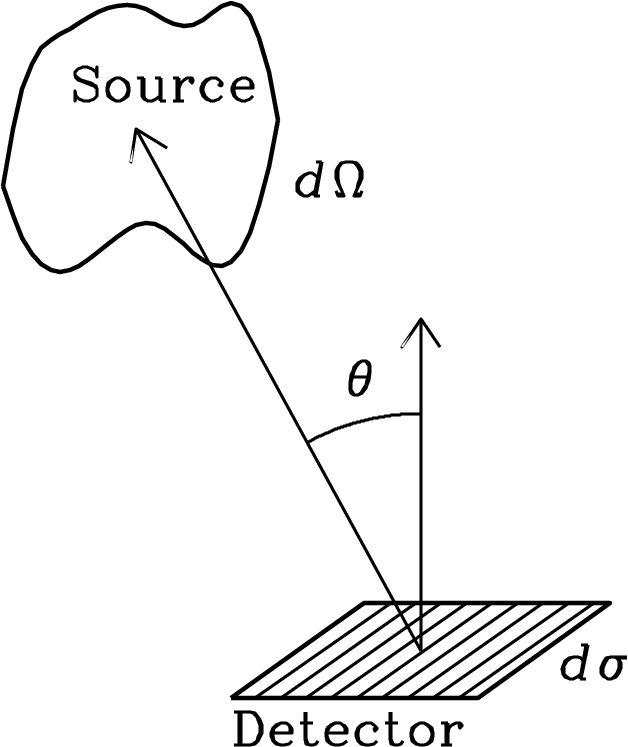
\includegraphics[width=0.3\textwidth]{specific-intensity}
  \bicaption{%
    \acl*{I-nu} \acs*{I-nu} 的测量示意图
  }{%
    The specific intensity \acs*{I-nu} measured by a detector of area
    $\D{\sigma}$ to a source extending a solid angle of $\D{\Omega}$.
    \\来源/Credit:
    \citeay{condon2016}, \S\,2.1
  }
  \label{fig:intensity}
\end{figure}

考虑一个面积为 $\D{\sigma}$ 的探测器,测量一个与其法线方向呈 $\theta$ 角度、
所张立体角为 $\D{\Omega}$ 的辐射源,如\autoref{fig:intensity} 所示。
若探测器在频率范围 $[\nu, \,\nu+\D{\nu}]$ 内接收到的功率为 $\D{P_{\nu}}$,
则这个源的\acl{I-nu} (specific intensity) \ac{I-nu} 定义为:
\begin{equation}
  \label{eq:intensity}
  \ac{I-nu} \equiv
    \frac{\D{P_{\nu}}}{(\cos\theta\,\D{\sigma}) \,\D{\nu} \,\D{\Omega}} \,,
\end{equation}
其 \ac{si} 单位是 [\si{\watt\per\square\meter\per\hertz\per\steradian}]。
\acl{I-nu} \ac{I-nu} 亦被称为\ac{spec-brightness},
有时也被简称为强度或亮度。

\begin{figure}[htp]
  \centering
  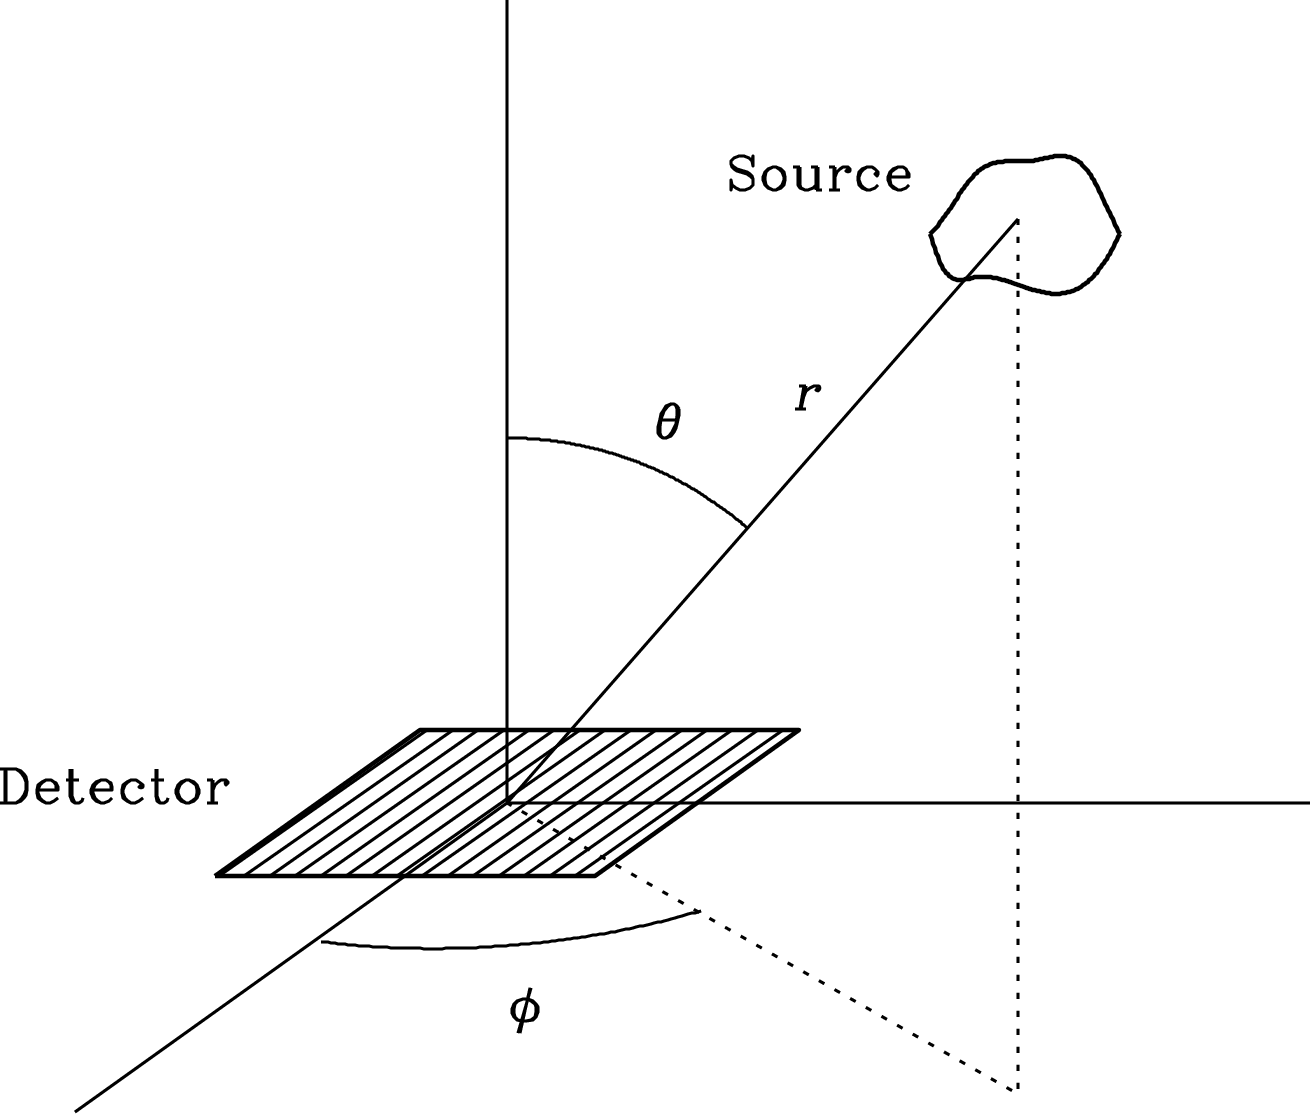
\includegraphics[width=0.6\textwidth]{flux-density}
  \bicaption{%
    \acl*{S-nu} \acs*{S-nu} 的定义示意图
  }{%
    An illustration of the definition of flux density \acs*{S-nu}.
    \\来源/Credit:
    \citeay{condon2016}, \S\,2.1
  }
  \label{fig:flux-density}
\end{figure}

一个\ac{src-discrete}所张的立体角是确定的(如\autoref{fig:flux-density} 所示),
因此探测器单位投影面积上接收到的\ac{spec-power}即为
这个源的\acl{S-nu} (flux density) \ac{S-nu}:
\begin{equation}
  \label{eq:flux-density}
  \ac{S-nu} \equiv
    \int_{\R{source}} \ac{I-nu}(\theta,\phi) \cos\theta \,\D{\Omega} ,
\end{equation}
其 \ac{si} 单位是 [\si{\watt\per\square\meter\per\hertz}]。
实际中常用单位 [\si{\jansky}],换算关系为
$\SI{1}{\jansky} = \SI{e-26}{\watt\per\square\meter\per\hertz}$。

一个辐射场的\acl{u-nu} (spectral energy density) 是指
每单位体积的\ac{spec-energy},具有 \ac{si} 单位
[\si{\joule\per\cubic\meter\per\hertz}]。
取辐射场中的一个体积元 $\D{V}$,对于来自某一方向的立体角元 $\D{\Omega}$
的一束辐射 $\ac{I-nu}(\theta,\phi)$,
可认为该体积元 $\D{V}$ 具有长度 $\D{s}$ 以及横截面积 $\D{\sigma}$,
即 $\D{V} = \D{s}\,\D{\sigma}$,
于是这束辐射 $\acs{I-nu}(\theta,\phi)$ 贡献给这个体积元的谱能量为:
\begin{equation}
  \D{\acs{u-nu}}\,\D{V}
    = \acs{I-nu}(\theta,\phi) \,\D{\Omega}\,\D{\sigma}
      \left( \frac{\D{s}}{\acs{speed-light}} \right) ,
\end{equation}
其中 \acs{speed-light} 是\acl{speed-light}。
所以源自 $\D{\Omega}$ 方向的辐射 $\acs{I-nu}(\theta,\phi)$
在体积元 $\D{V}$ 的位置贡献的\acl{u-nu}为:
\begin{equation}
  \D{\acs{u-nu}}
    = \frac{\acs{I-nu}(\theta,\phi)}{\acs{speed-light}} \,\D{\Omega} ,
\end{equation}
将上式对所有方向积分,即得辐射场的\acl{u-nu}:
\begin{equation}
  \label{eq:spectral-energy-density}
  \acs{u-nu}
    = \int_{4\Cpi} \D{\acs{u-nu}}
    = \frac{1}{\acs{speed-light}}
      \int_{4\Cpi} \acs{I-nu}(\theta,\phi) \,\D{\Omega} .
\end{equation}
如果辐射场是各向同性的,即 $\acs{I-nu}(\theta,\phi) = \acs{I-nu}$,则有:
\begin{equation}
  \label{eq:spectral-energy-density-iso}
  \acs{u-nu} = \frac{4\Cpi \, \acs{I-nu}}{\acs{speed-light}} .
\end{equation}

%---------------------------------------------------------------------
\subsection{辐射转移方程和光深}
\label{sec:radiative-transfer}

\begin{figure}[htp]
  \centering
  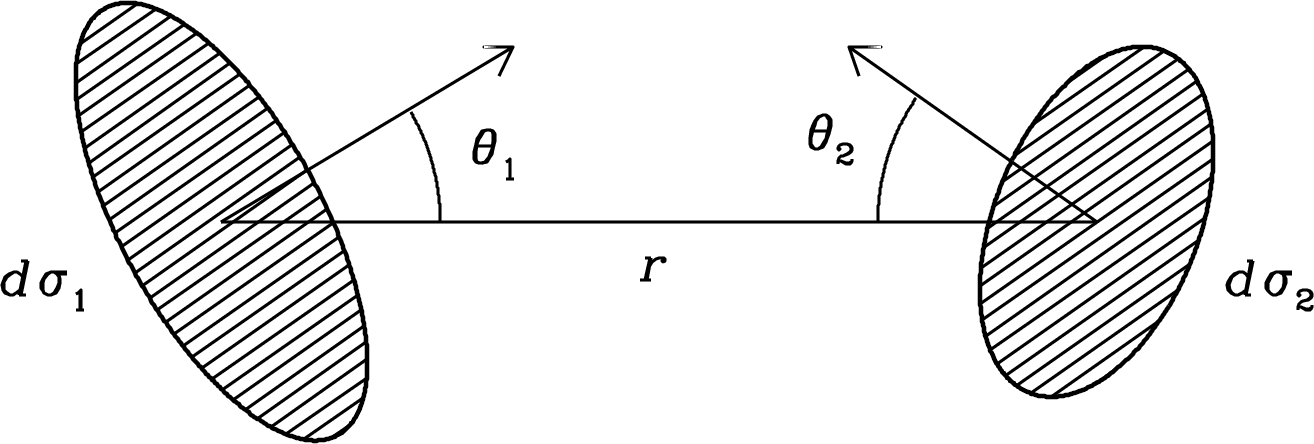
\includegraphics[width=0.6\textwidth]{specific-intensity-conservation}
  \bicaption{%
    \acl*{I-nu} \acs*{I-nu} 在自由空间里沿光线保持不变
  }{%
    The specific intensity \acs*{I-nu} conserved along a ray in empty space.
    \\来源/Credit:
    \citeay{condon2016}, \S\,2.1
  }
  \label{fig:intensity-conservation}
\end{figure}

辐射在不存在吸收和发射的自由空间里传播时强度保持不变,
即辐射的\acl*{I-nu} \acs*{I-nu} 与传播距离无关。
为说明这一点,考虑由源发射的一束光线,
设 $\D{\sigma_1}$ 和 $\D{\sigma_2}$ 是光线上相距为 $r$ 的两个面元
(如\autoref{fig:intensity-conservation} 所示),
则两个面元相互所张的立体角分别为:
\begin{align}
  \D{\Omega_1} & = \frac{\cos\theta_2 \,\D{\sigma_2}}{r^2} , \\
  \D{\Omega_2} & = \frac{\cos\theta_1 \,\D{\sigma_1}}{r^2} .
\end{align}
于是可知在频率范围 $[\nu, \,\nu+\D{\nu}]$ 以及立体角 $\D{\Omega_1}$ 之内
流过面元 $\D{\sigma_1}$ 的功率为:
\begin{align}
  \D{P_1} & = (\acs{I-nu})_1 \cos\theta_1
      \,\D{\Omega_1} \,\D{\sigma_1} \,\D{\nu}  \\
    & = (\acs{I-nu})_1 \left( \frac{\cos\theta_1 \cos\theta_2}{r^2} \right)
      \,\D{\sigma_1} \,\D{\sigma_2} \,\D{\nu} ,
\end{align}
类似地,流过面元 $\D{\sigma_2}$ 的功率为:
\begin{align}
  \D{P_2} & = (\acs{I-nu})_2 \cos\theta_2
      \,\D{\Omega_2} \,\D{\sigma_2} \,\D{\nu}  \\
    & = (\acs{I-nu})_2 \left( \frac{\cos\theta_1 \cos\theta_2}{r^2} \right)
      \,\D{\sigma_1} \,\D{\sigma_2} \,\D{\nu} .
\end{align}
根据能量守恒,即 $\D{P_1}\,\D{t} = \D{P_2}\,\D{t}$,
可得:
\begin{equation}
  \label{eq:intensity-conservation}
  (\acs{I-nu})_1 = (\acs{I-nu})_2 .
\end{equation}

\begin{figure}[htp]
  \centering
  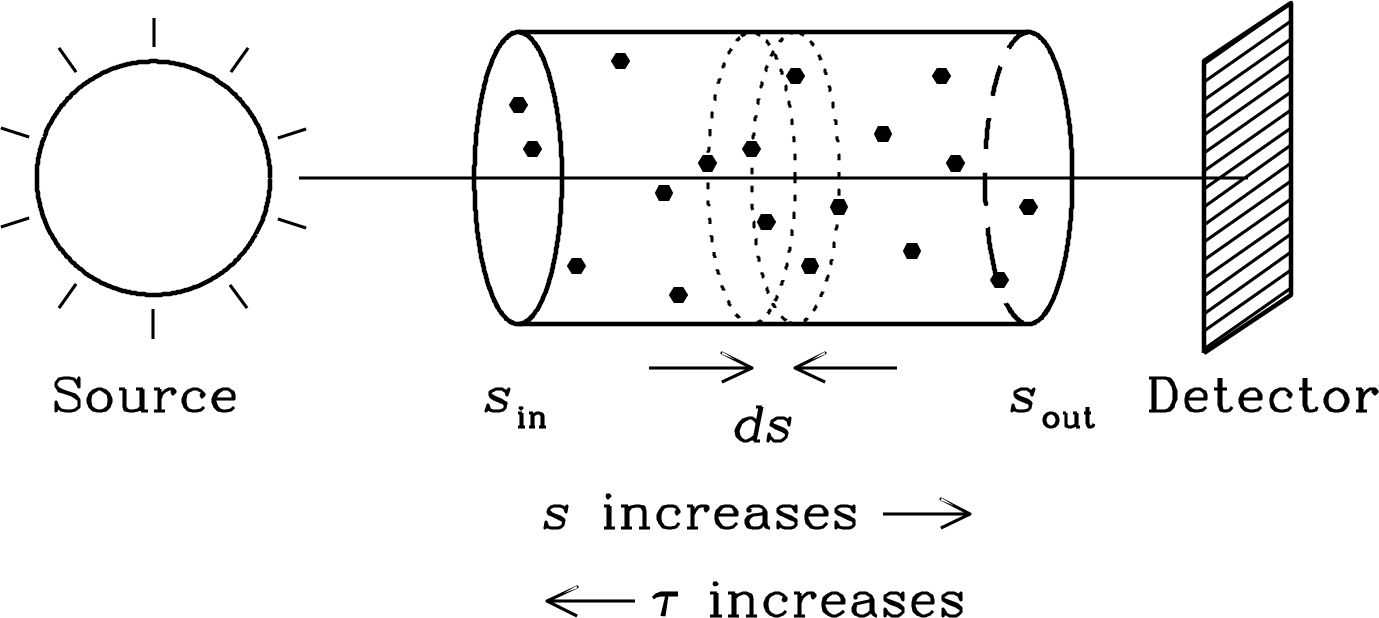
\includegraphics[width=0.6\textwidth]{radiative-transfer}
  \bicaption[辐射转移示意图]{%
    辐射转移示意图。
    距离 $s$ 沿源向探测器的方向增长,介质的入端和出端的距离分别为
    $s_{\R{in}}$ 和 $s_{\R{out}}$。
    光深 $\tau$ 的增长方向与 $s$ 相反。
  }{%
    An illustration of the radiative transfer.
    The distance $s$ increases along the ray from the source to the detector.
    The distances at the input end and the output end of the intervening
    medium are $s_{\R{in}}$ and $s_{\R{out}}$, respectively.
    The optical depth $\tau$ is measured in the opposite direction as $s$.
    \\来源/Credit:
    \citeay{condon2016}, \S\,2.2
  }
  \label{fig:radiative-transfer}
\end{figure}

当传播空间中存在吸收和发射时(如\autoref{fig:radiative-transfer} 所示),
辐射的\acl{I-nu} \acs{I-nu} 会发生改变,具体变化可由\acf{rt}方程描述。
首先考虑吸收情形,一个辐射光子通过介质中一个厚度为 $\D{s}$ 的薄层时被吸收的概率 $\D{p}$ 为:
\begin{equation}
  \D{p} = \acs{coef-absorption} \,\D{s} ,
\end{equation}
其中 \acs{coef-absorption}
为\acl{coef-absorption} (absorption coefficient),
具有 \ac{si} 单位 [\si{\per\meter}]。
于是\acl{I-nu} \acs{I-nu} 在通过厚度 $\D{s}$ 的介质后的损失比例为:
\begin{equation}
  \label{eq:rt-absorption}
  \frac{\D{\acs{I-nu}}}{\acs{I-nu}} = - \acs{coef-absorption} \,\D{s} .
\end{equation}
对上式的两边沿介质的吸收路径积分,可得:
\begin{equation}
  \int_{s_{\R{in}}}^{s_{\R{out}}} \frac{\D{\acs{I-nu}}}{\acs{I-nu}}
    = \ln\acs{I-nu} \,\Big|_{s_{\R{in}}}^{s_{\R{out}}}
    = - \int_{s_{\R{in}}}^{s_{\R{out}}} \acs{coef-absorption}(s') \,\D{s'} ,
\end{equation}
即
\begin{equation}
  \label{eq:intensity-loss1}
  \frac{\acs{I-nu}(s_{\R{out}})}{\acs{I-nu}(s_{\R{in}})} =
    \exp \left[ - \int_{s_{\R{in}}}^{s_{\R{out}}}
      \acs{coef-absorption}(s') \,\D{s'} \right] .
\end{equation}
据此,可定义\acl{optical-depth} (optical depth) 为:
\begin{equation}
  \label{eq:optical-depth}
  \acs{optical-depth} \equiv
    - \int_{s_{\R{out}}}^{s_{\R{in}}} \acs{coef-absorption}(s') \,\D{s'} .
\end{equation}
注意,上式的积分方向与 $s$ 相反(参见\autoref{fig:radiative-transfer}),
如此可使 $\tau > 0$ 并且与介质的观测深度成正相关。
利用\acl{optical-depth} \acs{optical-depth},
可将\autoref{eq:intensity-loss1} 写成:
\begin{equation}
  \label{eq:intensity-loss}
  \frac{\acs{I-nu}(s_{\R{out}})}{\acs{I-nu}(s_{\R{in}})} =
    \exp (-\acs{optical-depth}) .
\end{equation}
当 $\tau \ll 1$ 时,称介质是光学薄的;
当 $\tau \gg 1$ 时,则称介质是光学厚的。

另一方面,介质可能产生辐射而增大\acl{I-nu} \acs{I-nu}。
考虑介质中的一个体积元 $\D{s}\,\D{\sigma}$,在频率范围 $[\nu, \,\nu+\D{\nu}]$ 内
沿某一方向的立体角元 $\D{\Omega}$ 所发射的谱功率为:
\begin{equation}
  \D{P_{\nu}} =
    \acs{coef-emission} \,\D{s}\,\D{\sigma}\,\D{\nu}\,\D{\Omega} ,
\end{equation}
其中 \acs{coef-emission} 为\acl{coef-emission} (emission coefficient),
在不存在吸收的情况下可表示为:
\begin{equation}
  \label{eq:coef-emission}
  \acs{coef-emission} = \diff{\acs{I-nu}}{s} ,
\end{equation}
具有 \ac{si} 单位 [\si{\watt\per\cubic\meter\per\hertz\per\steradian}]。
综合上式和\autoref{eq:rt-absorption},可得完整的\ac{rt}方程为:
\begin{equation}
  \label{eq:radiative-transfer}
  \diff{\acs{I-nu}}{s} =
    - \acs{coef-absorption} \,\acs{I-nu} + \acs{coef-emission} .
\end{equation}

%---------------------------------------------------------------------
\subsection{热平衡和 Kirchhoff 定律}

\acf{te},简称热平衡,
是指一个系统在没有外界影响的条件下,其各部分的宏观属性在长时间内不发生任何变化的状态。
这是热力学的一个基本实验定律,是定义温度的基础。

\begin{figure}[htp]
  \centering
  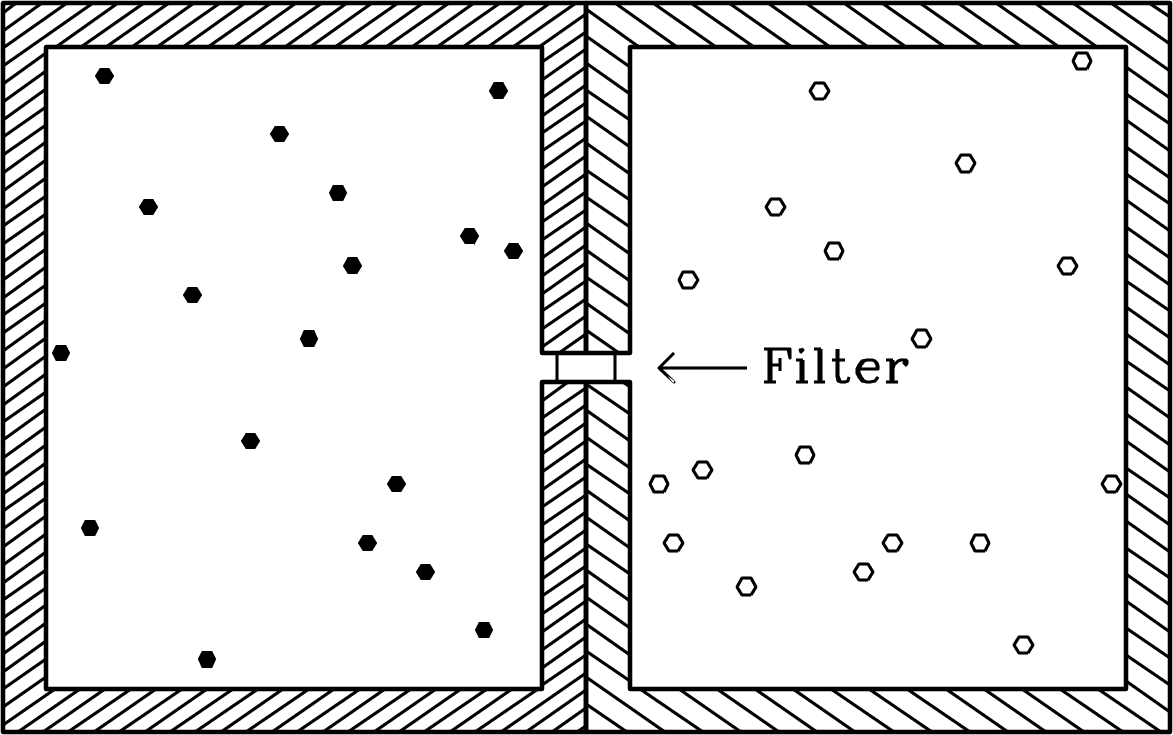
\includegraphics[width=0.5\textwidth]{Kirchhoff-law-experiment}
  \bicaption{%
    推导 Kirchhoff 定律的思想实验
  }{%
    A thought experiment to derive the Kirchhoff's law.
    \\来源/Credit:
    \citeay{condon2016}, \S\,2.2
  }
  \label{fig:kirchhoff-experiment}
\end{figure}

考虑如下思想实验:
两个由不同材料制成、包含不同介质的空腔放在一起,
中间由一个仅允许频率在 $[\nu, \,\nu+\D{\nu}]$ 之间的辐射通过的阀门连接,
如\autoref{fig:kirchhoff-experiment} 所示。
在完全热平衡的情形下,即空腔中的介质和辐射场具有相同的温度,
空腔产生的辐射与黑体辐射(详见后文 \autoref{sec:blackbody})相同,
完全由温度决定,而与其材质或者内部介质无关。
当两个空腔在任意温度 $T$ 达到完全热平衡时,
没有净能量从一个空腔通过阀门进入到另一个空腔,
否则损失能量的空腔将会冷却,另一个空腔将会升温,从而违背热力学第二定律。
由此可知:
\begin{align}
  \diff{\acs{I-nu}}{s} & = 0 , \\
  \acs{I-nu} & = B_{\nu}(T) ,
  \label{eq:kirchhoff-I-B}
\end{align}
其中 $B_{\nu}(T)$ 为空腔的辐射频谱。
于是辐射转移方程 [\autoref{eq:radiative-transfer}] 成为:
\begin{equation}
  \diff{\acs{I-nu}}{s} = 0
    = - \acs{coef-absorption} \,B_{\nu}(T) + \acs{coef-emission} ,
\end{equation}
所以:
\begin{equation}
  \label{eq:kirchhoff-law}
  \frac{\acs{coef-emission}(T)}{\acs{coef-absorption}(T)} = B_{\nu}(T) ,
\end{equation}
上式对任意频率 $\nu$ 均成立。
这就是完全热平衡系统的 Kirchhoff 定律。

完全热平衡状态只有在特殊的条件下才能实现;
对于一般的系统,介质无法与辐射场达到热平衡。
尽管如此,如果介质本身是热平衡的,则称该系统处于\acf{lte}状态。
对于这类\acf{lte}系统,Kirchhoff 定律 [\autoref{eq:kirchhoff-law}] 同样适用,
但是辐射场的\acl{I-nu} \ac{I-nu} 与介质的辐射频谱 $B_{\nu}(T)$ 通常不相等
(即\autoref{eq:kirchhoff-I-B} 不成立)。

%---------------------------------------------------------------------
\subsection{黑体辐射和亮温度}
\label{sec:blackbody}

黑体是一个能够吸收全部入射辐射而不产生任何反射或透射的理想化物体。
处于热力学平衡态的黑体所发出的辐射称为黑体辐射,其能谱分布只取决于黑体的温度,
由 Planck 辐射定律给出:
\begin{equation}
  \label{eq:planck}
  B_{\nu}(\nu, T) = \frac{2 \acs{hp} \nu^3}{\acs{speed-light}^2}
    \left[ \exp\left( \frac{\acs{hp} \nu}{\acs{kb} T} \right) - 1 \right]^{-1} ,
\end{equation}
其中 $B_{\nu}$ 是在频率 $\nu$ 处的谱亮度,
\acs{hp} 是 \acl{hp},
\acs{kb} 是 \acl{kb},
\acs{speed-light} 是\acl{speed-light}。

在射电波段,$\acs{hp}\nu \ll \acs{kb}T$ 通常成立,因此上式可近似为:
\begin{equation}
  \label{eq:rj-approx}
  B_{\nu}(\nu, T)
    \approx \frac{2 \nu^2 \acs{kb} T}{\acs{speed-light}^2} .
\end{equation}
这就是 Rayleigh--Jeans 近似。
在该近似下,黑体的谱亮度 $B_{\nu}$ 与其温度 $T$ 严格成正比。
因此,一个源的亮度(即\acl{I-nu}) \ac{I-nu}
可以很方便地使用\acl{T-b} (brightness temperature) \ac{T-b} 来描述:
\begin{equation}
  \label{eq:Tb}
  \acs{T-b}(\nu)
    \equiv \frac{\acs{I-nu} \acs{speed-light}^2}{2 \,\acs{kb} \nu^2} .
\end{equation}
对于一般的辐射源,其\acl{T-b} \ac{T-b} 会随频率 $\nu$ 发生改变。

%---------------------------------------------------------------------
\subsection{电阻的热噪声}

一个温度为 $T$ 的电阻 (resistor) 会因为内部电子的随机热运动而产生一个噪声,
称为 Johnson--Nyquist 噪声 \cite{johnson1928,nyquist1928},
其\ac{spec-power}由以下 Nyquist 近似给出
(详见 \citeay{condon2016}, \S\,2.5):
\begin{equation}
  \label{eq:nyquist-approx}
  P_{\nu} \approx \acs{kb} T .
\end{equation}
该式是 Rayleigh--Jeans 近似 [\autoref{eq:rj-approx}] 在电子学中的对应。
类似地,该近似公式只适用于 $\acs{hp}\nu \ll \acs{kb}T$ 的经典范畴。
在考虑量子化修正后,严格的 Nyquist 公式为:
\begin{equation}
  \label{eq:nyquist}
  P_{\nu} = \acs{hp} \nu
    \left[ \exp\left( \frac{\acs{hp} \nu}{\acs{kb} T} \right) - 1 \right]^{-1} .
\end{equation}


%=====================================================================
\section{谱线辐射基础}
\label{sec:spectral-line}

\acf{spec-line}是光谱上的窄($\Delta\nu \ll \nu$)发射或吸收特征,
源自原子或分子的能级跃迁。
当一个原子或分子从高能级 $E_2$ 跃迁至低能级 $E_1$ 时,会发射一个特定频率的光子,
一群这样的光子便形成了一条发射线 (emission line)。
反过来,如果一个原子或分子从低能级 $E_1$ 跃迁至高能级 $E_2$,
则会吸收一个特定频率的光子。
这些被吸收的光子通常来自背景的连续谱辐射,
因此观测到的连续谱上将出现一条吸收线 (absorption line)。
典型的谱线包括\ac{hii}的复合线、中性氢的 21\,cm 超精细结构谱线
(详见 \autoref{sec:21cm-line})。

%---------------------------------------------------------------------
\subsection{Einstein 系数和细致平衡方程}

\begin{figure}[htp]
  \centering
  
\includegraphics[width=0.9\textwidth]{atom-radiation-interactions}
  \bicaption[原子与辐射场的三种相互作用过程]{%
    原子与辐射场的三种相互作用过程:
    \emph{(a)} \acs*{em-spontaneous};
    \emph{(b)} \acs*{em-stimulated};
    \emph{(c)} 吸收。
  }{%
    The three processes that an atom interacts with the radiation field:
    \emph{(a)} spontaneous emission;
    \emph{(b)} stimulated emission;
    \emph{(c)} absorption.
  }
  \label{fig:atom-interactions}
\end{figure}

原子发射和吸收电磁辐射的量子理论是 Niels Bohr 在 1913 年提出的 \cite{bohr1913},
接着 Albert Einstein 在 1916 年提出了原子与辐射场的三种相互作用过程
\cite{einstein1916},分别为:
\begin{enumerate}
\item \emph{\acf{em-spontaneous}}:
  在没有外界光子的情况下,处在高能级 $E_2$ 的原子自发地跃迁到低能级 $E_1$
  而发射光子的过程 [如\autoref{fig:atom-interactions}(a) 所示]。
  发射光子的频率为 $\nu_0 = \Delta E / \acs{hp} = (E_2 - E_1) / \acs{hp}$。
  此类跃迁的速率正比于原子在高能级 $E_2$ 的布居数 $N_2$,即:
  \begin{equation}
    \label{eq:rate-em-spontaneous}
    \left( \diff{N_{21}}{t} \right)_{\R{sp}} = \ac{coef-A21} N_2 ,
  \end{equation}
  其中 \ac{coef-A21} 为\acl{coef-A21}。

\item \emph{\acf{em-stimulated}}:
  在频率为 $\nu_0$ 的外界光子的激励下,处在高能级 $E_2$ 的原子向低能级 $E_1$
  跃迁而发射光子的过程 [如\autoref{fig:atom-interactions}(b) 所示]。
  该过程产生的光子与入射光子具有相同的频率、相位、传播方向和偏振态等性质,
  这就是\acf{laser}的基本原理。
  这个过程的跃迁速率正比于原子在高能级 $E_2$ 的布居数 $N_2$
  以及辐射场的\acl{u-nu} $\acs{u-nu}(\nu_0)$,即:
  \begin{equation}
    \label{eq:rate-em-stimulated}
    \left( \diff{N_{21}}{t} \right)_{\R{st}}
      = \ac{coef-B21} N_2 \, \acs{u-nu}(\nu_0) ,
  \end{equation}
  其中 \ac{coef-B21} 为\acl{coef-B21}。

\item \emph{吸收}:
  处在低能级 $E_1$ 的原子吸收一个频率为 $\nu_0$ 的光子而跃迁到高能级 $E_2$ 的过程
  [如\autoref{fig:atom-interactions}(c) 所示]。
  类似地,该过程的跃迁速率正比于原子在低能级 $E_1$ 的布居数 $N_1$
  以及辐射场的\acl{u-nu} $\acs{u-nu}(\nu_0)$,即:
  \begin{equation}
    \label{eq:rate-absorption}
    \diff{N_{12}}{t} = \ac{coef-B12} N_1 \, \acs{u-nu}(\nu_0) ,
  \end{equation}
  其中 \ac{coef-B12} 为\acl{coef-B12}。
\end{enumerate}
以上三个公式中的比例系数 \ac{coef-A21}、\ac{coef-B21} 和 \ac{coef-B12}
统称为 Einstein 系数。

考虑一个处于完全热平衡的原子系统,
则能级 $E_1$ 和 $E_2$ 之间的三种跃迁过程应满足\acf{detailed-balance}条件:
\begin{equation}
  \label{eq:detailed-balance1}
  \left( \diff{N_{21}}{t} \right)_{\R{sp}}
    + \left( \diff{N_{21}}{t} \right)_{\R{st}} = \diff{N_{12}}{t} ,
\end{equation}
即有:
\begin{equation}
  \label{eq:detailed-balance2}
  A_{21} N_2 + B_{21} N_2 \, \acs{u-nu}(\nu_0)
    = B_{12} N_1 \, \acs{u-nu}(\nu_0) .
\end{equation}
同时,原子在两个能级上的布居数服从 Boltzmann 分布:
\begin{equation}
  \label{eq:ratio-populations-te}
  \frac{N_2}{N_1}
    = \frac{g_2}{g_1} \exp\left( - \frac{E_2-E_1}{\acs{kb} T} \right)
    = \frac{g_2}{g_1} \exp\left( - \frac{\acs{hp} \nu_0}{\acs{kb} T} \right) ,
\end{equation}
其中 $T$ 为系统的热力学温度,
$g_1$ 和 $g_2$ 分别为能级 $E_1$ 和 $E_2$ 的\acf{dod}。

从\autoref{eq:detailed-balance2} 可解出辐射场的\acl{u-nu}:
\begin{equation}
  \acs{u-nu}(\nu_0) = \frac{A_{21}}{(N_1/N_2) B_{12} - B_{21}} ,
\end{equation}
代入\autoref{eq:ratio-populations-te} 可进一步得到:
\begin{equation}
  \label{eq:radiation-spec1}
  \acs{u-nu}(\nu_0) = A_{21} \left[ \frac{g_1}{g_2} B_{12}
    \exp\left( \frac{\acs{hp} \nu_0}{\acs{kb} T} \right)
    - B_{21} \right]^{-1} .
\end{equation}

另一方面,辐射场的频谱 $B_{\nu}(T)$ 由 Planck 辐射定律 [\autoref{eq:planck}] 给出,
再根据\autoref{eq:spectral-energy-density-iso},可知辐射场的\acl{u-nu}为:
\begin{equation}
  \label{eq:radiation-spec2}
  \acs{u-nu}(\nu_0) = \frac{4\Cpi}{\acs{speed-light}}
    \frac{2 \acs{hp} \nu_0^3}{\acs{speed-light}^2}
    \left[ \exp\left( \frac{\acs{hp} \nu_0}{\acs{kb} T} \right)
      - 1 \right]^{-1} .
\end{equation}
联合上式和\autoref{eq:radiation-spec1},可得
\begin{equation}
  \frac{A_{21}}{B_{21}} \left[ \frac{g_1}{g_2} \frac{B_{12}}{B_{21}}
    \exp\left( \frac{\acs{hp} \nu_0}{\acs{kb} T} \right) - 1 \right]^{-1}
  = \frac{8\Cpi \acs{hp} \nu_0^3}{\acs{speed-light}^3}
    \left[ \exp\left( \frac{\acs{hp} \nu_0}{\acs{kb} T} \right)
      - 1 \right]^{-1} .
\end{equation}
上式必须对任意温度 $T$ 均成立,因此可导出:
\begin{equation}
  \label{eq:detailed-balance}
  \left\{
    \begin{aligned}
      \frac{g_1}{g_2} \frac{B_{12}}{B_{21}} & = 1 , \\
      \frac{A_{21}}{B_{21}} & =
        \frac{8\Cpi \acs{hp} \nu_0^3}{\acs{speed-light}^3} .
    \end{aligned}
  \right.
\end{equation}
这就是描述三个 Einstein 系数相互关联的\ac{detailed-balance}方程。
只要知道任何一个 Einstein 系数,就可以据此导出另外两个系数。

%---------------------------------------------------------------------
\subsection{含 Einstein 系数的辐射转移方程}

在考虑辐射转移时,介质的性质由\acl{coef-emission} \acs{coef-emission}
和\acl{coef-absorption} \acs{coef-absorption} 描述。
对于谱线的\ac{rt}问题,
\acs{coef-emission} 和 \acs{coef-absorption} 均可使用 Einstein 系数表示出来。
利用\ac{detailed-balance}方程 [\autoref{eq:detailed-balance}],
可进一步只使用\acl{coef-A21} \ac{coef-A21} 来表示这两个系数。

考虑一个在能级 $E_1$ 和 $E_2$ 之间跃迁的热平衡系统,
原子(或分子)在这两个能级上的布居数密度分别为 $N_1$ 和 $N_2$。
对于系统中的一个体积元 $\D{V} = \D{s}\,\D{\sigma}$,
在时间 $\D{t}$、频率范围 $[\nu, \,\nu+\D{\nu}]$、
沿某一方向的立体角元 $\D{\Omega}$ 内通过\ac{em-spontaneous}过程产生的能量为:
\begin{equation}
  \D{E_{\R{sp}}(\nu)}
    = \acs{hp} \nu_0 A_{21} N_2 \,\phi(\nu)
      \,\D{V}\,\D{t}\,\D{\nu} \left( \frac{\D{\Omega}}{4\Cpi} \right) ,
\end{equation}
其中 $\nu_0 = (E_2 - E_1) / \acs{hp}$ 为谱线的中心频率,
$\phi(\nu)$ 为\acf{line-profile}。
类似地,体积元 $\D{V}$ 通过\ac{em-stimulated}过程产生的能量为:
\begin{equation}
  \D{E_{\R{st}}(\nu)}
    = \acs{hp} \nu_0 B_{21} N_2 \acs{u-nu} \,\phi(\nu)
      \,\D{V}\,\D{t}\,\D{\nu} \left( \frac{\D{\Omega}}{4\Cpi} \right) ,
\end{equation}
以及吸收的能量为:
\begin{equation}
  \D{E_{\R{ab}}(\nu)}
    = \acs{hp} \nu_0 B_{12} N_1 \acs{u-nu} \,\phi(\nu)
      \,\D{V}\,\D{t}\,\D{\nu} \left( \frac{\D{\Omega}}{4\Cpi} \right) ,
\end{equation}
其中
$\acs{u-nu} = 4\Cpi\,\acs{I-nu} / \acs{speed-light}$
为辐射场的\acl{u-nu} [参见\autoref{eq:spectral-energy-density-iso}]。
在热平衡的情形下,有
\begin{equation}
  \D{E_{\R{sp}}(\nu)} + \D{E_{\R{st}}(\nu)} - \D{E_{\R{ab}}(\nu)}
    = \D{\acs{I-nu}}\,\D{\sigma}\,\D{t}\,\D{\nu}\,\D{\Omega} ,
\end{equation}
即为含 Einstein 系数的\ac{rt}方程:
\begin{equation}
  \diff{\acs{I-nu}}{s}
    = - \left [ \frac{\acs{hp} \nu_0}{\acs{speed-light}}
      (B_{12} N_1 - B_{21} N_2) \phi(\nu) \right] \acs{I-nu}
      + \frac{\acs{hp} \nu_0}{4\Cpi} A_{21} N_2 \,\phi(\nu) .
\end{equation}
对比 \autoref{sec:radiative-transfer} 所述的辐射转移方程
[\autoref{eq:radiative-transfer}],
可得\acl{coef-emission} \acs{coef-emission}
和\acl{coef-absorption} \acs{coef-absorption} 分别为:
\begin{align}
  \acs{coef-emission}
    & = \frac{\acs{hp} \nu_0}{4\Cpi} A_{21} N_2 \,\phi(\nu) ,
  \label{eq:coef-emission-einstein} \\
  \acs{coef-absorption}
    & = \frac{\acs{hp} \nu_0}{\acs{speed-light}}
      (B_{12} N_1 - B_{21} N_2) \phi(\nu) .
  \label{eq:coef-absorption-einstein1}
\end{align}

将\ac{detailed-balance}方程 [\autoref{eq:detailed-balance}]
代入上述两式,可得:
\begin{equation}
  \label{eq:emission-absorption-ratio1}
  \frac{\acs{coef-emission}}{\acs{coef-absorption}}
    = \frac{2 \acs{hp} \nu_0^3}{\acs{speed-light}^2}
      \left( \frac{g_2}{g_1} \frac{N_1}{N_2} - 1 \right)^{-1} .
\end{equation}
对于局部热平衡的系统,Kirchhoff 定律 [\autoref{eq:kirchhoff-law}] 给出:
\begin{equation}
  \label{eq:emission-absorption-ratio2}
  \frac{\acs{coef-emission}}{\acs{coef-absorption}}
    = B_{\nu}(T)
    = \frac{2 \acs{hp} \nu_0^3}{\acs{speed-light}^2} \left[
      \exp\left( \frac{\acs{hp} \nu_0}{\acs{kb} T} \right) - 1 \right]^{-1} ,
\end{equation}
其中使用了 Planck 辐射定律 [\autoref{eq:planck}]。
比较\autoref{eq:emission-absorption-ratio1}
和\autoref{eq:emission-absorption-ratio2},可得:
\begin{equation}
  \label{eq:ratio-populations-lte}
  \frac{N_2}{N_1}
    = \frac{g_2}{g_1} \exp\left( -\frac{\acs{hp} \nu_0}{\acs{kb} T} \right) .
\end{equation}
这说明处于局部热平衡的系统的能级布居与完全热平衡的系统的情形
[\autoref{eq:ratio-populations-te}] 相同。
利用\autoref{eq:coef-emission-einstein}、
\autoref{eq:emission-absorption-ratio1}
以及\autoref{eq:ratio-populations-lte},
可以得到使用\acl{coef-A21} \ac{coef-A21}
表示的\acl{coef-absorption} \acs{coef-absorption}:
\begin{align}
  \acs{coef-absorption}
    & = \frac{\acs{speed-light}^2}{8\Cpi \nu_0^2} A_{21} N_2
      \left[ \exp\left( \frac{\acs{hp} \nu_0}{\acs{kb} T} \right) - 1 \right]
      \phi(\nu)
    \label{eq:coef-absorption-einstein2} \\
    & = \frac{\acs{speed-light}^2}{8\Cpi \nu_0^2} \frac{g_2}{g_1} A_{21} N_1
      \left[ 1 - \exp\left( -\frac{\acs{hp} \nu_0}{\acs{kb} T} \right) \right]
      \phi(\nu) .
    \label{eq:coef-absorption-einstein3}
\end{align}

%---------------------------------------------------------------------
\subsection{能级相对布居和激发温度}

即使一个二能级系统未处于局部热平衡状态,
仍然可以使用下式定义其\acl{T-excitation} (excitation temperature)
\ac{T-excitation}:
\begin{equation}
  \label{eq:t-excitation-def}
  \frac{N_2}{N_1} \equiv \frac{g_2}{g_1}
    \exp\left(- \frac{E_2-E_1}{\acs{kb} \acs{T-excitation}} \right)
    = \frac{g_2}{g_1}
      \exp\left( -\frac{\acs{hp} \nu_0}{\acs{kb} \acs{T-excitation}} \right) .
\end{equation}
该温度 \acs{T-excitation} 描述了两个能级的布居数 $N_2$ 和 $N_1$ 之比,
由系统的辐射、\ac{coll-excitation}和\ac{coll-deexcitation} 三者之间的平衡决定。

在单位时间、单位体积内,如果碰撞引发 $N_1 C_{12}$ 次从低能级 $E_1$ 到高能级 $E_2$
的激发和 $N_2 C_{21}$ 次从 $E_2$ 到 $E_1$ 的退激,
则系统的平衡条件成为:
\begin{equation}
  \label{eq:detailed-balance-collison1}
  N_2 [A_{21} + B_{21} \,\acs{u-nu}(\nu_0) + C_{21}]
    = N_1 [B_{12} \,\acs{u-nu}(\nu_0) + C_{12}] ,
\end{equation}
根据\ac{detailed-balance}条件 [\autoref{eq:detailed-balance2}] 可知:
\begin{equation}
  \label{eq:detailed-balance-collison2}
  N_1 C_{12} = N_2 C_{21} .
\end{equation}
联合\autoref{eq:radiation-spec2} 和\autoref{eq:detailed-balance} 可得:
\begin{equation}
  \label{eq:tex-coefs-b}
  B_{12} \,\acs{u-nu}(\nu_0)
    = \frac{g_2}{g_1} B_{21} \,\acs{u-nu}(\nu_0)
    = A_{21} \frac{g_2}{g_1} \left[ \exp\left(
        \frac{\acs{hp} \nu_0}{\acs{kb} T_b} \right) - 1 \right]^{-1} ,
\end{equation}
其中 $T_b$ 为辐射场的\acl{T-b}。
再利用\autoref{eq:ratio-populations-lte}
和\autoref{eq:detailed-balance-collison2} 可得:
\begin{equation}
  \label{eq:tex-coefs-c}
  C_{12} = \frac{g_2}{g_1} C_{21}
    \exp\left( - \frac{\acs{hp} \nu_0}{\acs{kb} \acs{T-kinetic}} \right) ,
\end{equation}
其中 \acs{T-kinetic} 为系统(通常为气体)的\acl{T-kinetic}。
将\autoref{eq:tex-coefs-b} 和\autoref{eq:tex-coefs-c}
代入\autoref{eq:detailed-balance-collison1},整理可得:
\begin{equation}
  \frac{N_2\,g_1}{N_1\,g_2} =
    \frac{A_{21} + C_{21}
    \exp\left( -\frac{\acs{hp} \nu_0}{\acs{kb} \acs{T-kinetic}} \right)
      \left[ \exp\left( \frac{\acs{hp} \nu_0}{\acs{kb} T_b} \right)
        - 1 \right]
    }{A_{21} \exp\left( \frac{\acs{hp} \nu_0}{\acs{kb} T_b} \right)
     + C_{21} \left[ \exp\left( \frac{\acs{hp} \nu_0}{\acs{kb} T_b}
       \right) - 1 \right]} .
\end{equation}
最后将上式代入\autoref{eq:t-excitation-def},
得到\acl{T-excitation} \acs{T-excitation} 与 \acs{T-b} 和 \acs{T-kinetic}
之间的关系为:
\begin{equation}
  \label{eq:t-excitation}
  \exp\left(- \frac{\acs{hp} \nu_0}{\acs{kb} \acs{T-excitation}} \right) =
    \exp\left( -\frac{\acs{hp} \nu_0}{\acs{kb} T_b} \right)
    \frac{A_{21} + C_{21} \exp\left(
      -\frac{\acs{hp} \nu_0}{\acs{kb} \acs{T-kinetic}} \right)
      \left[ \exp\left( \frac{\acs{hp} \nu_0}{\acs{kb} T_b} \right)
        - 1 \right]
    }{A_{21} + C_{21} \left[ 1 - \exp\left(
      -\frac{\acs{hp} \nu_0}{\acs{kb} T_b} \right) \right]} .
\end{equation}
从上式可以看出,
如果辐射占主导 ($A_{21} \gg C_{21}$),
则\acl{T-excitation}趋近于辐射场的\acl{T-b} ($\acs{T-excitation} \to T_b$);
反之,如果碰撞占主导 ($A_{21} \ll C_{21}$),
则\acl{T-excitation}趋近于介质的\acl{T-kinetic}
($\acs{T-excitation} \to \acs{T-kinetic}$)。


%=====================================================================
\section{基本天线概念}
\label{sec:antenna}

天线可分为接收型(如射电望远镜)和发射型(如雷达)两类。
前者接收外界的电磁波将其转换成电信号,后者则将输入的电信号转换成电磁波发射出去。
在种类繁多的天线中,短偶极天线是其中最基本的一种,
下文对其进行简要介绍,并以此天线为例介绍若干重要的天线概念。

%---------------------------------------------------------------------
\subsection{短偶极天线的辐射场}

短偶极天线由两个总长度 $l$ 远小于波长 $\lambda$ 的导体组成
(\autoref{fig:short-dipole} 所示)。
当接上一个交流驱动电源后,导体内的电子会发生往复的加速运动,从而激发电磁波。

\begin{figure}[htp]
  \centering
  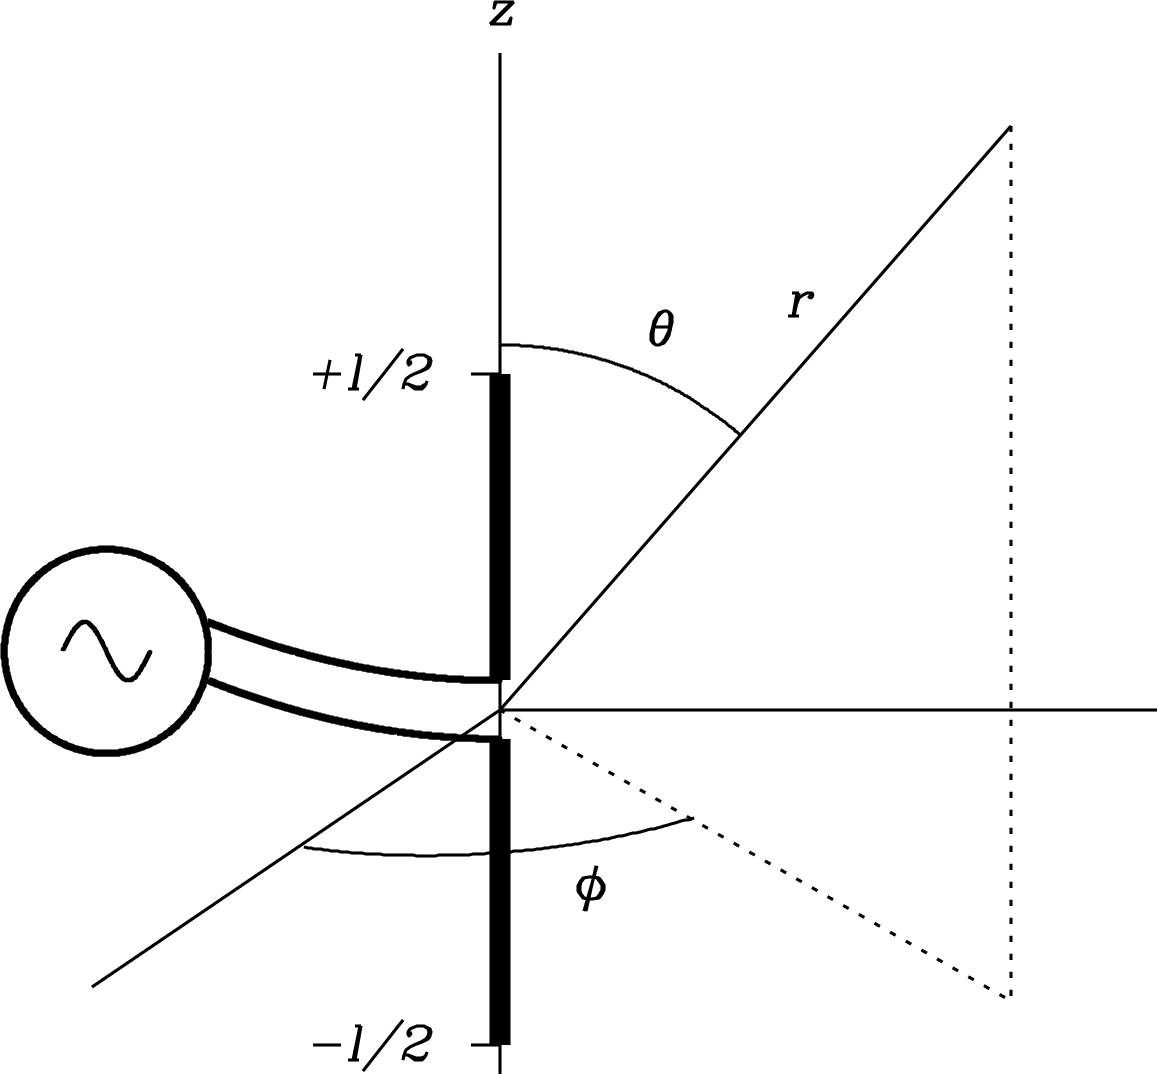
\includegraphics[width=0.5\textwidth]{short-dipole}
  \bicaption[短偶极天线示意图]{%
    分析短偶极天线的辐射所采用的坐标系统。
  }{%
    The coordinate system used to describe the radiation from a
    short dipole.
    \\来源/Credit:
    \citeay{condon2016}, \S\,3.1.1
  }
  \label{fig:short-dipole}
\end{figure}

首先考虑一个加速度为 $\dot{v}$ 的电荷 $q$,在距离 $r$ 处产生的切向
(即与 $r$ 的方向垂直)电场强度为
(详见 \citeay{condon2016}, \S\,2.7):
\begin{equation}
  \label{eq:q-efield}
  E_{\perp} = \frac{q \dot{v} \sin\theta}{r \acs{speed-light}^2} ,
\end{equation}
其中
\acs{speed-light} 是\acl{speed-light},
$\theta$ 为 $r$ 与 $v$ 之间的夹角。
天线的每一小段 $\D{z}$ 均会贡献一定的电场强度 $\D{E_{\perp}}$,
由于 $l \ll \lambda$,因此产生的总电场强度为:
\begin{equation}
  \label{eq:dipole-efield1}
  E_{\perp} = \int_{-l/2}^{l/2}
    \frac{\dot{v} \sin\theta}{r \acs{speed-light}^2} \,\diff{q}{z}\D{z} .
\end{equation}
对于远场情形 ($r \gg l$),$1/r$ 可视为常数而提出积分号。
考虑一个正弦形式的驱动电流:
\begin{equation}
  \label{eq:dipole-current}
  I = I_0 \Ce^{-\Ci \omega t} ,
\end{equation}
其中 $I_0$ 为电流峰值,
于是 $\dot{v} = -\Ci \omega v$。
导线中的电流可表示为:
\begin{equation}
  \label{eq:wire-current}
  I \equiv \diff{q}{t} = \diff{q}{z} \diff{z}{t} = \diff{q}{z} v ,
\end{equation}
代入\autoref{eq:dipole-efield1},可得
\begin{align}
  \label{eq:dipole-efield2}
  E_{\perp}
    & = -\frac{\Ci\omega \sin\theta}{r \acs{speed-light}^2}
      \int_{-l/2}^{l/2} \diff{q}{z} v \,\D{z} \\
    & = -\frac{\Ci\omega \sin\theta}{r \acs{speed-light}^2}
      \int_{-l/2}^{l/2} I\,\D{z} .
\end{align}
从天线的中点到两端,电流近似线性地减小至 0,即导线中的电流分布为:
\begin{equation}
  \label{eq:dipole-current-dist}
  I(z) \approx I_0 \Ce^{-\Ci\omega t}
    \left[ 1 - \frac{|z|}{l/2} \right] .
\end{equation}
最终可得天线在 $r$ 处产生的切向电场强度为:
\begin{align}
  E_{\perp}
    & \approx -\frac{\Ci\omega \sin\theta}{r \acs{speed-light}^2}
      \frac{I_0 l}{2} \Ce^{-\Ci\omega t} \\
    & = -\frac{\Ci\Cpi \sin\theta}{r \acs{speed-light}}
      \frac{I_0 l}{\lambda} \Ce^{-\Ci\omega t} .
    \label{eq:dipole-efield}
\end{align}
\autoref{fig:dipole-radiation} 显示了一个无限短偶极天线(即 Hertz 偶极子)
的瞬时电场强度分布图。

\begin{figure}[htp]
  \centering
  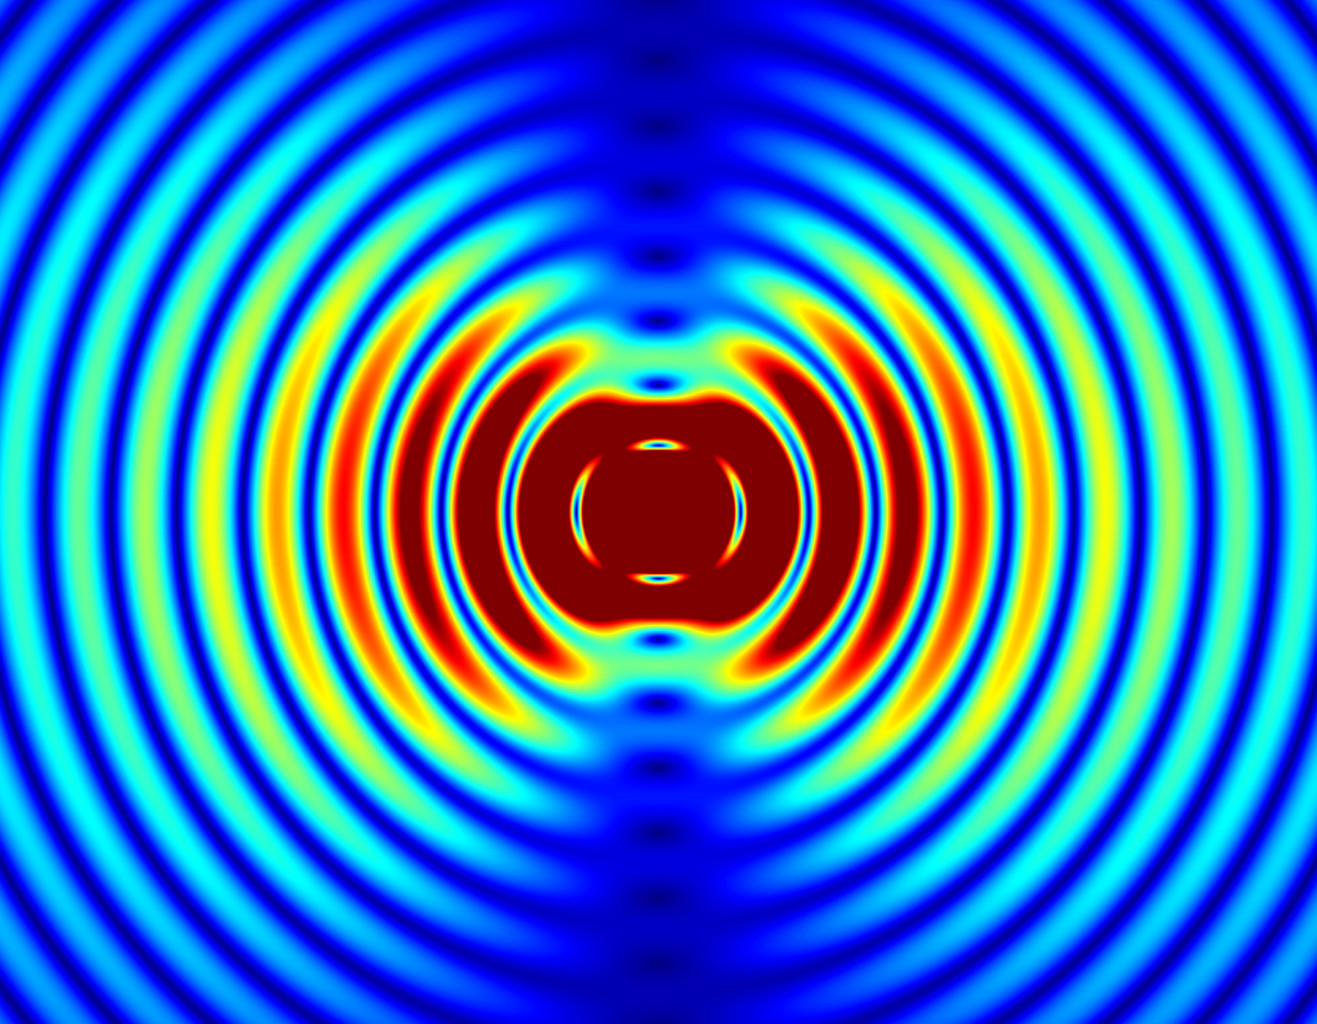
\includegraphics[width=0.6\textwidth]{hertzian-dipole-radiation}
  \bicaption{%
    Hertz 偶极子的瞬时电场强度分布图
  }{%
    The instantaneous electric field intensity distribution of
    a Hertzian dipole.
    \\来源/Credit:
    nageljr, \url{https://www.deviantart.com/nageljr/art/The-Hertzian-Dipole-Antenna-542377463}, (2019-03-18), \ac{cc} BY
  }
  \label{fig:dipole-radiation}
\end{figure}

%---------------------------------------------------------------------
\subsection{功率方向图和增益}

\acf{pp} $P(\theta,\phi)$ 是指一个天线的辐射功率的角向分布。
对于短偶极天线,由\autoref{eq:dipole-efield} 可得对时间平均的
Poynting 流量(即单位面积流过的功率)为:
\begin{equation}
  \label{eq:poynting-flux}
  \langle S \rangle
    = \frac{\acs{speed-light}}{4\Cpi} \langle E_{\perp}^2 \rangle
    = \frac{\Cpi}{8\,\acs{speed-light}}
      \left( \frac{I_0 l}{\lambda} \right)^2 \frac{\sin^2\theta}{r^2} .
\end{equation}
于是该天线的\ac{pp} $P(\theta,\phi)$ 为:
\begin{equation}
  P(\theta,\phi) = \langle S \rangle.
\end{equation}
在实际情况中,一般使用归一化的\ac{pp},即:
\begin{align}
  \label{eq:power-pattern}
  P_n(\theta,\phi)
    & \equiv P(\theta,\phi) / P_{\R{max}} \\
    & = \sin^2\theta .
\end{align}
对于更一般的天线,其\ac{pp} $P(\theta,\phi)$
将与两个空间方位角 $(\theta, \phi)$ 均相关。

\acf{gain} $G(\theta,\phi)$ 定义为天线在方向 $(\theta, \phi)$
的辐射功率 $P(\theta,\phi)$ 与一个总辐射功率相等但各向辐射同性的天线的辐射功率
$\bar{P}$ 之比,即:
\begin{equation}
  \label{eq:gain}
  G(\theta,\phi) = \frac{P(\theta,\phi)}{\bar{P}}
    = \frac{4\Cpi P(\theta,\phi)}{\int P(\theta,\phi) \,\D{\Omega}} .
\end{equation}
可见,天线的\ac{gain}与其\ac{pp}只相差一个常数。
对于一个理想的天线,全天平均的增益为:
\begin{equation}
  \label{eq:gain-avg}
  \langle G \rangle
    \equiv \frac{1}{4\Cpi} \int G(\theta,\phi) \,\D{\Omega}
    = 1 .
\end{equation}
在实际应用中,\ac{gain} $G$ 通常使用 [\si{\decibel}] 为单位:
\begin{equation}
    G_{\si{\decibel}} \equiv 10 \log_{10} G .
\end{equation}

%---------------------------------------------------------------------
\subsection{主瓣及其\acl*{hpbw}}

天线的\ac{pp} $P(\theta,\phi)$ 通常会在某个方向范围内具有
比在其他方向明显更大的值,
这个方向范围便称为天线的\acf{mainlobe},
其余方向的辐射瓣则称为\acf{sidelobe},如\autoref{fig:lobes} 所示。
主瓣的立体角 $\Omega_{\R{MB}}$ 定义为:
\begin{equation}
  \label{eq:omega-mb}
  \Omega_{\R{MB}} = \int_{\R{MB}} P_n(\theta,\phi) \,\D{\Omega} ,
\end{equation}
其中 $P_n(\theta,\phi)$ 为归一化的\ac{pp} [\autoref{eq:power-pattern}]。
主瓣的角度范围一般由\acf{hpbw}描述,定义为 $P(\theta,\phi)$
下降至最大值的一半时主瓣的两点之间的角距离(\autoref{fig:lobes})。
若天线的辐射越具有方向性,则天线的\ac{gain} $G$ 越大,
主瓣的立体角 $\Omega_{\R{MB}}$ 越小,\ac{hpbw} 也越小。

\begin{figure}[htp]
  \centering
  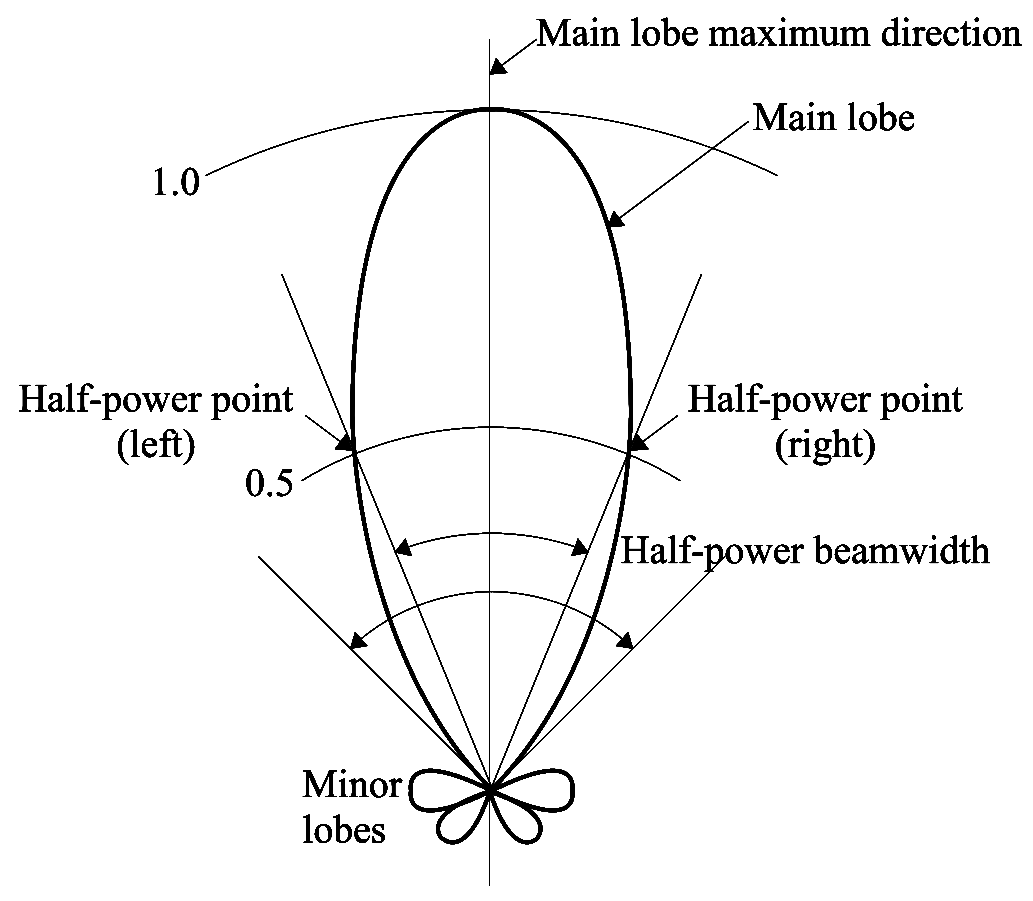
\includegraphics[width=0.6\textwidth]{antenna-lobes}
  \bicaption{%
    天线主瓣及其\acl*{hpbw} (HPBW) 的示意图
  }{%
    Diagram of an antenna's main lobe and its HPBW.
    \\来源/Credit:
    \citeay{zuniga2009}
  }
  \label{fig:lobes}
\end{figure}

%---------------------------------------------------------------------
\subsection{有效接收面积}

在测量一个流量密度为 $S_{\nu}$ 的无偏振源时,
若天线输出的谱功率为 $P_{\nu}$,
则该天线的\acl{area-eff} (effective collecting area) \ac{area-eff}
定义为:
\begin{equation}
  \label{eq:area-eff}
  \ac{area-eff} \equiv \frac{2 P_{\nu}}{S_{\nu}} ,
\end{equation}
式中的因子 \enquote{2} 是因为单个天线只能响应一个偏振方向。

\begin{figure}[htp]
  \centering
  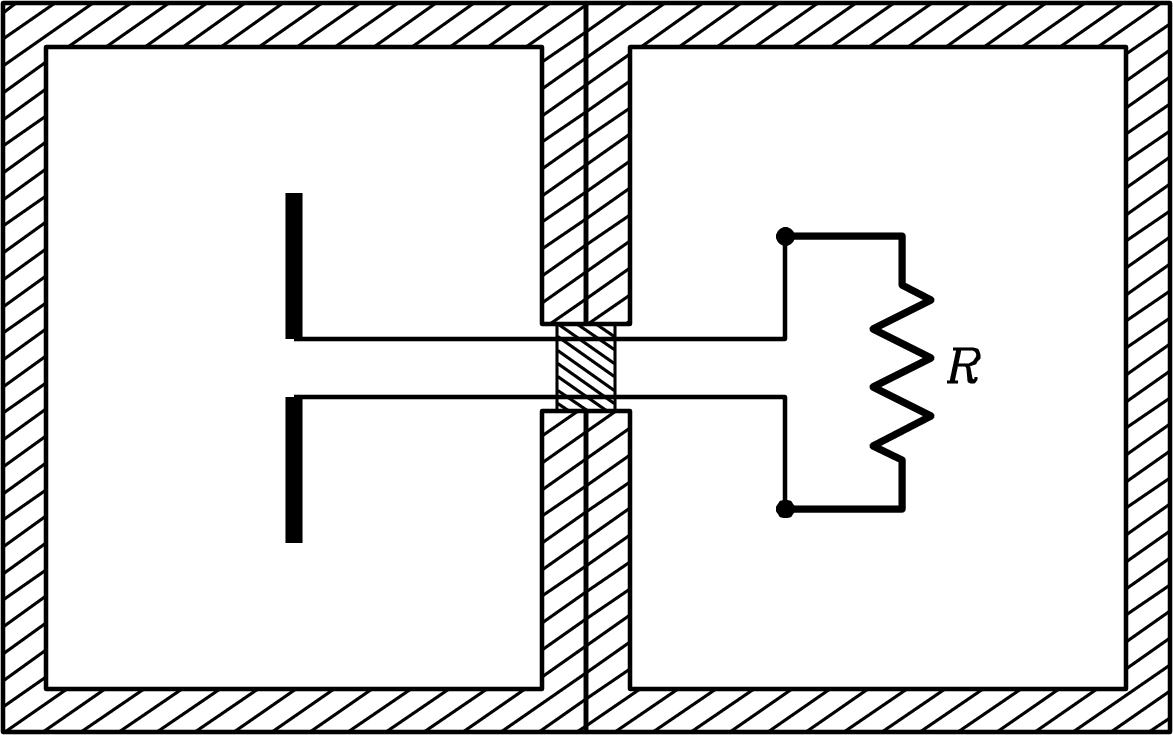
\includegraphics[width=0.5\textwidth]{average-area-thought-exp}
  \bicaption{%
    计算天线平均接收面积 $\langle \ac*{area-eff} \rangle$ 的思想实验
  }{%
    A thought experiment to calculate the average collection area
    $\langle \ac*{area-eff} \rangle$ of an antenna.
    \\来源/Credit:
    \citeay{condon2016}, \S\,3.1.4
  }
  \label{fig:area-avg-exp}
\end{figure}

天线的平均接收面积定义为:
\begin{equation}
  \label{eq:area-avg1}
  \langle \ac{area-eff} \rangle
    \equiv \frac{1}{4\Cpi} \int \ac{area-eff}(\theta,\phi) \,\D{\Omega} .
\end{equation}
为计算该面积,可借助这样一个思想实验:
一个理想的天线和一个理想的电阻,分别置于两个温度均为 $T$ 的空腔中并且达到热平衡;
天线和电阻之间使用导线相连,两个空腔之间设有一个特殊的阀门,能够阻挡电磁波,
但允许频率范围为 $[\nu, \,\nu+\D{\nu}]$ 的电流通过导线,
如\autoref{fig:area-avg-exp} 所示。
因为整个系统处于热平衡状态,所以导线中没有净能量流动,
否则其中一个空腔将升温、另一个则冷却,违背热力学第二定律。
因此,天线接收各个方向的无偏振黑体辐射 $B_{\nu}(T)$ 所产生的\ac{spec-power}为:
\begin{equation}
  P_{\nu,a} =
    \frac{1}{2} \int \ac{area-eff}(\theta,\phi) B_{\nu}(T) \,\D{\Omega} ,
\end{equation}
而且该\ac{spec-power}必须等于电阻的热噪声的\ac{spec-power} $P_{\nu,r}$。
代入\autoref{eq:nyquist} 和\autoref{eq:planck},可得
\begin{equation}
  \acs{kb}T =
    \frac{2\,\acs{kb}T}{2\lambda^2}
      \int \ac{area-eff}(\theta,\phi) \,\D{\Omega} ,
\end{equation}
其中 $\lambda = \ac{speed-light} / \nu$ 为辐射的波长。
于是天线的平均接收面积 $\langle \ac{area-eff} \rangle$ 为:
\begin{equation}
  \label{eq:area-avg}
  \langle \ac{area-eff} \rangle = \frac{\lambda^2}{4\Cpi} ,
\end{equation}
因此不同形状、大小的理想天线均具有相同的平均接收面积。
由\ac{reciprocity-theorem}可知,同一个天线的发射\ac{pp}和接收\ac{pp}相同,即:
\begin{equation}
  G(\theta,\phi) \propto A_e(\theta,\phi) .
\end{equation}
结合\autoref{eq:area-avg} 和\autoref{eq:gain-avg}
可得天线在某个方向的\acl{area-eff}为:
\begin{equation}
  \ac{area-eff}(\theta,\phi) = \frac{\lambda^2 G(\theta,\phi)}{4\Cpi} .
\end{equation}
若天线的\acl{area-eff} $\ac{area-eff}(\theta,\phi)$ 越大,
则天线在此方向的\ac{gain} $G(\theta,\phi)$ 也越大,
于是天线的\ac{directivity}越强,对其他方向的灵敏度越低。

%---------------------------------------------------------------------
\subsection{天线温度}

一个被置于温度为 $T$ 的黑体辐射环境中的天线,
输出的噪声将与温度为 $T$ 的电阻所产生的热噪声 [\autoref{eq:nyquist-approx}]
相同(即具有相同的频谱),该电阻被称为天线的匹配电阻。
若天线的输出谱功率为 $P_{\nu}$,则其匹配电阻的温度为
$T_r = P_{\nu} / \acs{kb}$,
于是定义\acl{T-antenna} (antenna temperature) 为其匹配电阻的温度,即:
\begin{equation}
  \label{eq:t-ant}
  \acs{T-antenna} \equiv T_r = \frac{P_{\nu}}{\acs{kb}} .
\end{equation}
\acl{T-antenna} \ac{T-antenna} 与天线的物理温度没有必然联系,
仅作为天线测量值的一个方便表示。
这个概念被广泛使用的原因主要有:
\begin{itemize}
  \item $\acs{T-antenna} = \SI{1}{\kelvin}$ 对应的谱功率为
    $P_{\nu} = \SI{1.38e-23}{\watt\per\hertz}$,
    是一个实用的小量,便于表示实际测量结果;
  \item 天线系统通常使用不同温度的电阻(称为负载)来进行校准,
    因此\acl{T-antenna}能够自然地表示校准结果;
  \item 接收机的噪声也使用 [\si{\kelvin}] 为单位,
    因此采用\acl{T-antenna}来描述信号强度能够简化信号和噪声的比较。
\end{itemize}

设天线的有效接收面积为 \ac{area-eff} [\autoref{eq:area-eff}],
则一个流量密度为 $S_{\nu}$ 的无偏振辐射源将使天线的温度 \acs{T-antenna} 上升:
\begin{equation}
  \label{eq:dt-source}
  \Delta\acs{T-antenna} = \frac{\ac{area-eff} S_{\nu}}{2\,\acs{kb}} .
\end{equation}


%=====================================================================
\section{射电干涉测量的基本原理}
\label{sec:interferometry}

根据衍射原理,望远镜的角分辨率约为 $\theta \sim \lambda / D$,
其中 $\lambda$ 为信号的波长(对应于观测频率),$D$ 为望远镜的口径。
与光学波段相比,射电信号的波长要长得多。
为了实现足够好的角分辨率,必须建造巨型的望远镜,
比如 \SI{100}{\meter} 口径的 \ac{gbt}、
\SI{305}{\meter} 口径的 Arecibo、
\SI{500}{\meter} 口径的 \ac{fast}。
然而在数百 \si{\MHz} 的低频射电波段,望远镜的口径需达到惊人的 \SI{10}{\km} 左右
才能在 \SI{100}{\MHz} 实现约 \SI{1}{\arcminute} 的角分辨率,
这对于单口径望远镜而言显然是不现实的。
因此,低频射电观测通常使用\ac{interferometry}技术,
通过联合一系列小望远镜开展相干测量并综合,获得高分辨率图像。

%---------------------------------------------------------------------
\subsection{二元单色干涉仪}

\begin{figure}[htp]
  \centering
  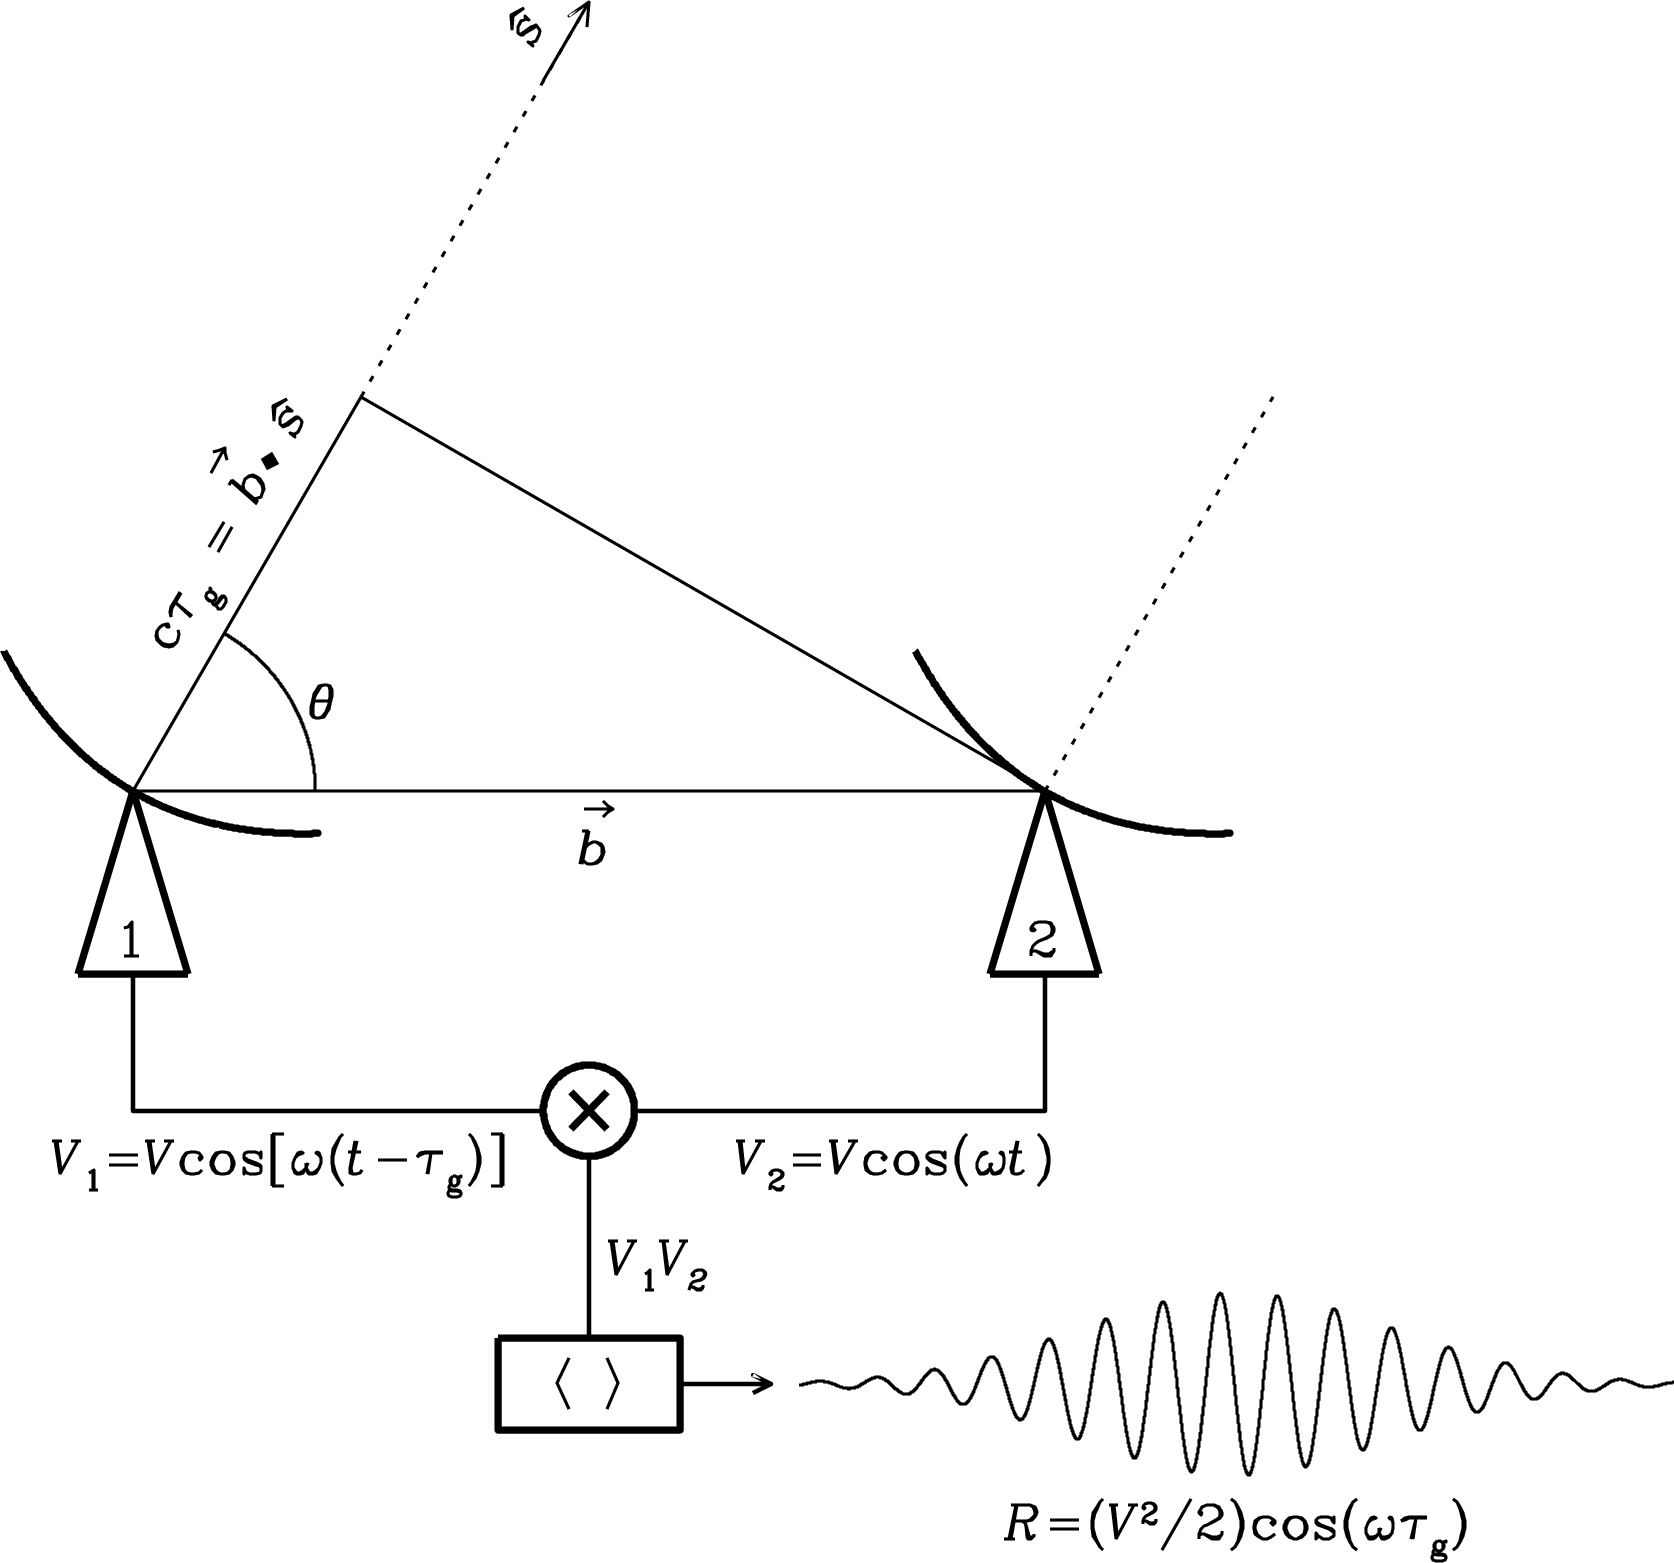
\includegraphics[width=0.7\textwidth]{interferometer}
  \bicaption[二元单色干涉仪的构成示意图]{%
    二元单色干涉仪的构成示意图。
    两个相同的天线相距 \ac*{v-baseline} 放置并指向位于 \ac*{v-direction} 方向的辐射源,
    接收的信号被放大后,再经过\acs*{correlator}的相乘($\times$)
    和时间平均($\langle\;\rangle$),得到输出响应 $R$。
  }{%
    The components of a two-element quasi-monochromatic interferometer
    observing in a very narrow radio frequency band centered at
    $\nu = \omega / (2\Cpi)$.
    The two identical antennas are separated by the baseline vector
    \ac*{v-baseline} and point to the source in direction \ac*{v-direction}.
    The signals received by the antennas are amplified,
    multiplied ($\times$), and time averaged ($\langle\;\rangle$)
    by the correlator to yield the output response $R$.
    \\来源/Credit:
    \citeay{condon2016}, \S\,3.7.1
  }
  \label{fig:interferometer}
\end{figure}

考虑一个最简单的二元单色干涉仪(如\autoref{fig:interferometer} 所示),
由两个相同的天线和\ac{correlator}构成,只测量频率为 $\nu$ 的单色信号。
由于辐射源非常遥远,其信号到达干涉仪时为平面波(忽略电离层扰动等影响)。
同一个波面被两个天线接收的时刻之间存在一定的差异,
即为\acl{delay-geo} (geometric delay) \ac{delay-geo}:
\begin{equation}
  \acs{delay-geo} =
    \frac{\ac{v-baseline} \cdot \ac{v-direction}}{\acs{speed-light}} ,
\end{equation}
其中 \acs{speed-light} 是\acl{speed-light},
\ac{v-baseline} 为两天线之间的\acl{v-baseline}(由天线 1 指向天线 2),
\ac{v-direction} 为辐射源的\acl{v-direction}。
两个天线接收信号后输出的电压响应分别为:
\begin{equation}
  \left\{
    \begin{aligned}
      V_1(t) &= V \cos [\omega (t - \acs{delay-geo})] , \\
      V_2(t) &= V \cos (\omega t) ,
    \end{aligned}
  \right.
\end{equation}
其中 $\omega = 2\Cpi\nu$ 为角频率。
\ac{correlator}然后将两个天线的响应相乘:
\begin{align}
  V_1(t) V_2(t)
    &= V^2 \cos [\omega (t - \acs{delay-geo})] \cos (\omega t) \\
    &= \frac{1}{2} V^2 \left[ \cos (2\omega t - \omega \acs{delay-geo})
      + \cos (\omega \acs{delay-geo}) \right] ,
\end{align}
接着再进行时间平均:
\begin{equation}
  \label{eq:resp-corr}
  R = \langle V_1(t) V_2(t) \rangle
    = \frac{1}{2} V^2 \cos (\omega \acs{delay-geo}) .
\end{equation}
由于天线响应 $V_1$ 和 $V_2$ 正比于辐射源的亮度和天线的\ac{gain}
[参见\autoref{eq:gain}],
因此\ac{correlator}的响应 $R$ 正比于辐射源的流量密度 $S$
和 $\sqrt{A_1 A_2}$,其中 $A_1$ 和 $A_2$ 为两个天线的有效接收面积
[参见\autoref{eq:area-avg}]。

当辐射源的方向 \ac{v-direction} 改变时(比如由于地球的自转),
\acl{delay-geo} \acs{delay-geo} 也随之变化,
于是\ac{correlator}的输出 $R$ 出现正弦形式的振荡,
被称为干涉仪的响应\acf{fringe},
其相位为:
\begin{equation}
  \phi = \omega \acs{delay-geo}
    = 2\Cpi \left( \frac{b \cos\theta}{\lambda} \right) ,
\end{equation}
其中 $\theta$ 为\acl{v-direction} \ac{v-direction}
和\acl{v-baseline} \ac{v-baseline} 之间的夹角。
根据
\begin{equation}
  \diff{\phi}{\theta}
    = 2\Cpi \left( \frac{b \sin\theta}{\lambda} \right) ,
\end{equation}
可知单个\ac{fringe}的宽度 \acs{bw-synthesized} 为:
\begin{equation}
  \label{eq:bw-synthesized}
  \acs{bw-synthesized} = \frac{\lambda}{b \sin\theta} ,
\end{equation}
此参数称为干涉仪的\acl{bw-synthesized} (synthesized beamwidth),
描述了干涉仪的角分辨能力。

天线的\ac{pp}描述了天线响应随方向的变化情况,也被称为干涉仪的\acf{beam-primary},
将对输出 $R$ 产生调制,亦如\autoref{fig:interferometer} 所示,
其中\ac{correlator}的响应\ac{fringe}的\ac{envelope}示意了\ac{beam-primary}的衰减情况。

对于一个表面亮度分布为 $\acs{I-nu}(\ac{v-direction})$ 的\ac{src-extended},
由于不同位置产生的辐射互不相干,因此可以被当作一系列独立的点源处理,
于是上述二元单色干涉仪观测这个\ac{src-extended}的输出响应为:
\begin{align}
  R_c & = \int \acs{I-nu}(\ac{v-direction})
      \cos \left( \omega \ac{v-baseline} \cdot \ac{v-direction} /
        \acs{speed-light} \right)
      \,\D{\Omega}  \\
    & = \int \acs{I-nu}(\ac{v-direction}) \cos \left(
        2\Cpi\, \ac{v-baseline} \cdot \ac{v-direction} / \lambda \right)
      \,\D{\Omega} ,
    \label{eq:resp-cos}
\end{align}
其中下标 \enquote{$c$} 表示 \enquote{cosine} \ac{correlator}的输出,
以区分下文将要介绍的 \enquote{sine} \ac{correlator}。

一个任意的亮度分布 $I$ 可分解为奇对称成分 $I_{\R{odd}}$
与偶对称成分 $I_{\R{even}}$ 之和,
但是\autoref{eq:resp-cos} 描述的 cosine \ac{correlator}只能测量其中的
偶对称成分 $I_{\R{even}}$,因为:
\begin{align}
  R_c & = \int \left[ I_{\R{odd}}(\ac{v-direction}) +
        I_{\R{even}}(\ac{v-direction}) \right]
      \cos \left( 2\Cpi\, \ac{v-baseline} \cdot \ac{v-direction} /
        \lambda \right)
      \,\D{\Omega}  \\
    & = \int I_{\R{even}}(\ac{v-direction}) \cos \left(
        2\Cpi\, \ac{v-baseline} \cdot \ac{v-direction} / \lambda \right)
      \,\D{\Omega} .
\end{align}
为了能够测量另一个奇对称成分 $I_{\R{odd}}$,
则需要一个 \enquote{sine} \ac{correlator},
可通过对其中一个天线的输出增加 $\Cpi/2$ 的相位延迟来实现,于是有:
\begin{align}
  R_s & = \int \left[ I_{\R{odd}}(\ac{v-direction}) +
        I_{\R{even}}(\ac{v-direction}) \right]
      \sin \left( 2\Cpi\, \ac{v-baseline} \cdot \ac{v-direction} /
        \lambda \right)
      \,\D{\Omega}  \\
    & = \int I_{\R{odd}}(\ac{v-direction}) \sin \left(
        2\Cpi\, \ac{v-baseline} \cdot \ac{v-direction} / \lambda \right)
      \,\D{\Omega} .
\end{align}
一对 cosine 和 sine \ac{correlator}的组合称为\ac{c-correlator}。
因此\acl{Vis} (complex visibility),简称\ac{vis},可定义为:
\begin{align}
  \acs{Vis}
    & \equiv R_c - \Ci\, R_s  \\
    & = \int \ac{I-nu}(\ac{v-direction}) \exp
      (-2\Cpi\Ci\, \ac{v-baseline} \cdot \ac{v-direction} / \lambda)
      \,\D{\Omega} .
    \label{eq:vis}
\end{align}

%---------------------------------------------------------------------
\subsection{有限带宽和平均时间的影响}

将上述二元单色干涉仪推广至有限带宽信号的测量。
考虑一个中心频率为 $\nu_c$ 且宽度为 $\Delta\nu$ 的窄频带 ($\Delta\nu \gg \nu_c$),
可认为辐射源的亮度和天线的响应在此频带内保持不变,
于是可得干涉仪测量的\ac{vis} [\autoref{eq:vis}] 为:
\begin{align}
  \acs{Vis}
    & = \int \left[ \frac{1}{\Delta\nu}
        \int_{\nu_c-\Delta\nu/2}^{\nu_c+\Delta\nu/2}
        I(\ac{v-direction}, \nu) \exp (-2\Cpi\Ci\, \nu\acs{delay-geo})
      \right] \,\D{\Omega} \\
    & \approx \int \ac{I-nu}(\ac{v-direction})
      \sinc_{\Cpi} (\Delta\nu\,\acs{delay-geo})
      \exp (-2\Cpi\Ci\, \nu_c\acs{delay-geo}) \,\D{\Omega},
  \label{eq:vis-bw}
\end{align}
其中归一化 $\sinc_{\Cpi}$ 函数的定义如下:
\begin{equation}
  \label{eq:sinc}
  \sinc_{\Cpi}(x) =
    \begin{dcases*}
      \frac{\sin(\Cpi x)}{\Cpi x}, \quad & if $x \neq 0$, \\
      1, \quad & if $x = 0$.
    \end{dcases*}
\end{equation}
因此对于带宽为 $\Delta\nu$ 的非单色信号,
干涉仪测得的\ac{fringe}幅度减弱至原来的
$\sinc_{\Cpi}(\Delta\nu\,\acs{delay-geo})$ 倍。
为了尽可能地减小这种损失,可以给\enquote{前导}天线
(即先接收到信号的天线)的输出信号增加\acl{delay-comp}
(compensating delay) \ac{delay-comp}
(如\autoref{fig:interferometer-tau0} 所示),
使其满足 $|\acs{delay-comp} - \acs{delay-geo}| \ll (\Delta\nu)^{-1}$,
于是两个天线的输出响应到达\ac{correlator}时具有同步的相位。
满足 $\acs{delay-comp} = \acs{delay-geo}$ 的方向 $\ac{v-direction}_0$
称为\acf{delay-center}或\acf{phase-refpos}。

\begin{figure}[htp]
  \centering
  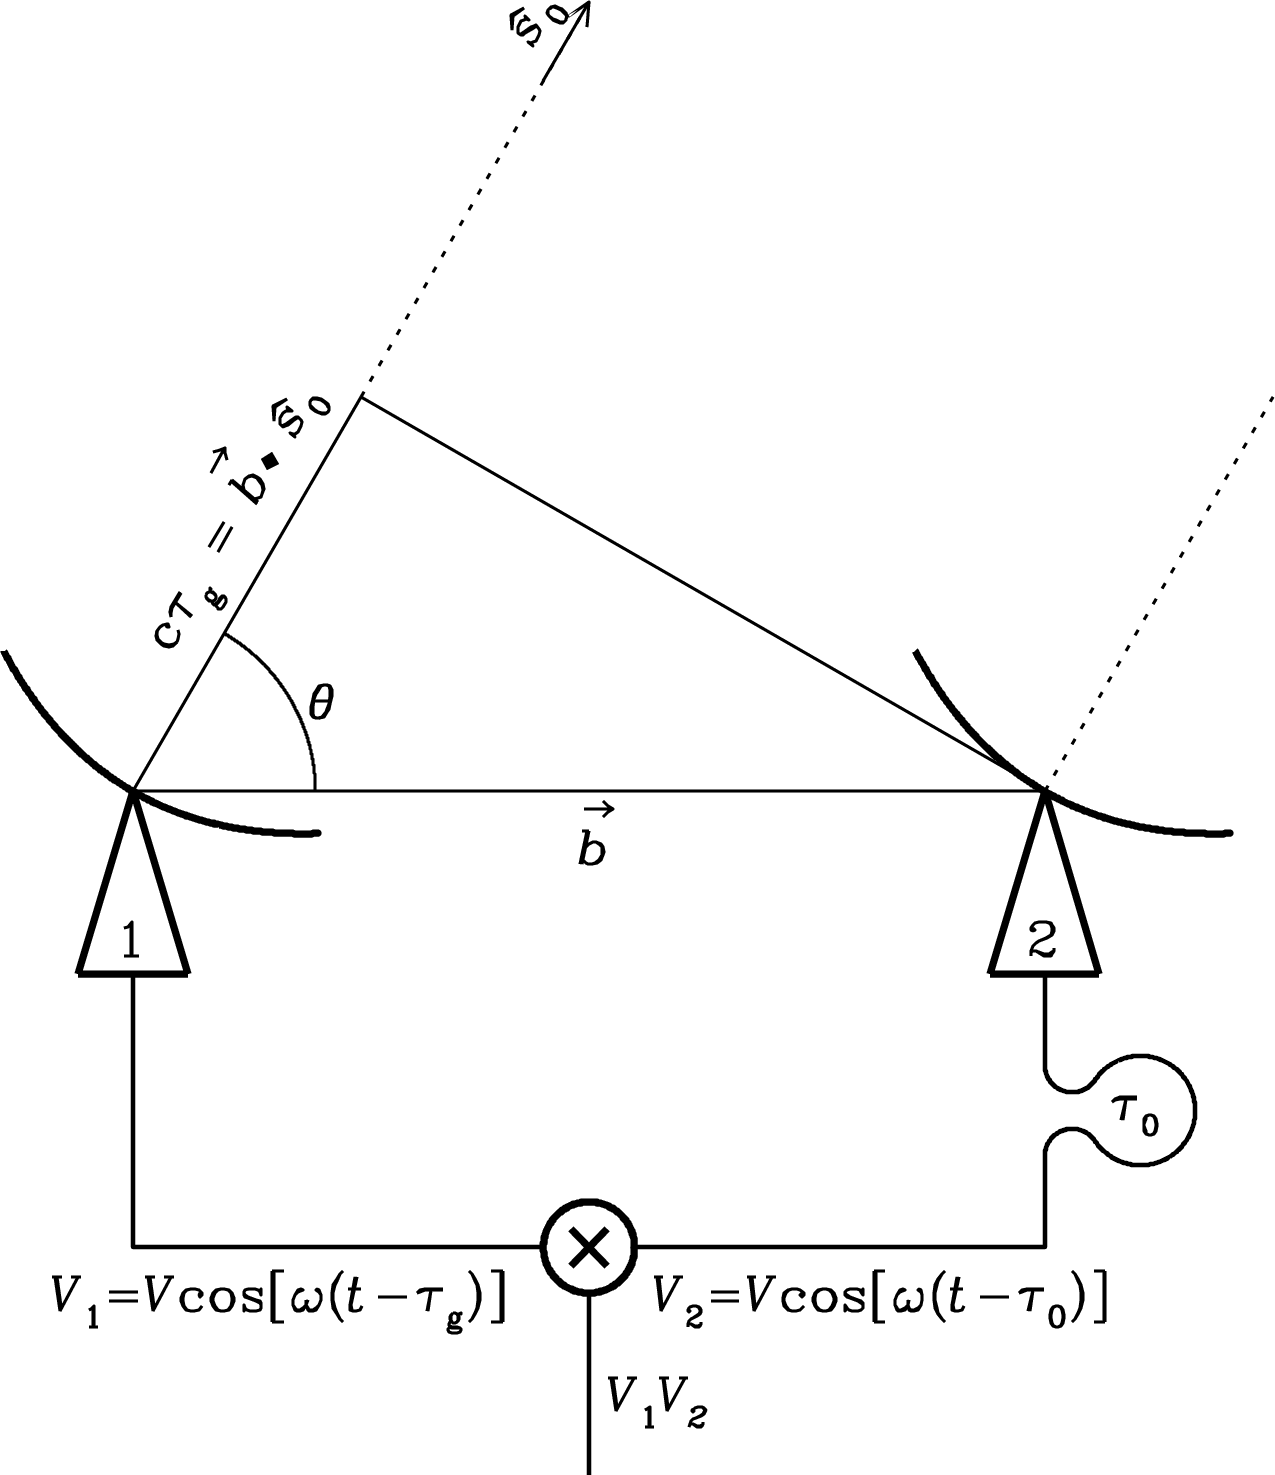
\includegraphics[width=0.6\textwidth]{interferometer-tau0}
  \bicaption[通过\acl*{delay-comp} \acs*{delay-comp} 来减小带宽效应的影响]{%
    通过给前导天线(对应于图中的天线 2)增加\acl*{delay-comp}
    $\acs*{delay-comp} \approx \acs*{delay-geo}$,
    使两个天线的输出信号的相位在相关运算时保持同步,
    从而最小化带宽效应的影响。
  }{%
    By introducing the compensating delay
    $\acs*{delay-comp} \approx \acs*{delay-geo}$ in the signal path of the
    leading antenna (i.e., the antenna 2), the phases of the two signals are
    almost in sync when they reach the correlator, hence minimizing the
    attenuation to the measured fringes caused by the finite bandwidth
    effect.
    \\来源/Credit:
    \citeay{condon2016}, \S\,3.7.3
  }
  \label{fig:interferometer-tau0}
\end{figure}

因为\acl{delay-geo} \acs{delay-geo} 会随方向 $\ac{v-direction}$ 而变化,
所以\acl{delay-comp} \acs{delay-comp} 只对特定方向 $\ac{v-direction}_0$
(即\ac{delay-center})是恰好准确的。
偏离\ac{delay-center}的角度 $\Delta\theta$ 越大,
\acl{delay-comp} \acs{delay-comp} 的修正效果就越差,
带宽效应产生的影响也就越严重。
这个效应被称为\acf{bw-smear},限制了有效的视场大小。
为了满足:
\begin{equation}
  \Delta\nu \Delta\acs{delay-geo}
    \approx \Delta\nu \diff{\acs{delay-geo}}{\theta} \Delta\theta
    = \frac{b \sin\theta}{\acs{speed-light}} \Delta\nu \Delta\theta
    \ll 1 ,
\end{equation}
则要求视场半径满足:
\begin{equation}
  \Delta\theta \ll \frac{\nu \acs{bw-synthesized}}{\Delta\nu} .
\end{equation}
另一个解决\ac{bw-smear}的方法是将一个宽频带划分为一系列足够窄(约几十 \si{\kHz})
的频率\ac{channel},然后对每个\ac{channel}的信号独立地进行相关运算得到\ac{vis}。

类似地,如果\ac{correlator}的\ac{t-avg} $\Delta t$ 过长,
则辐射源的位置 \ac{v-direction} 会因地球自转而发生显著改变
(可与 \acs{bw-synthesized} 相比拟),
导致\acl{delay-comp} \acs{delay-comp} 的修正效果变差。
这个效应被称为\acf{t-smear}。
一个距离\ac{delay-center} $\Delta\theta$ 的目标的移动速度为
$v = \omega_e \Delta\theta$,其中 $\omega_e$ 为地球自转的角速度。
为了最小化\ac{t-smear}的影响,\ac{correlator}的\ac{t-avg} $\Delta t$ 需满足:
\begin{equation}
  v \Delta t = \omega_e \Delta\theta \Delta t \ll \theta_s ,
\end{equation}
即:
\begin{equation}
  \label{eq:correlator-avgtime}
  \Delta t \ll \frac{\theta_s}{\omega_e \Delta\theta} .
\end{equation}

%---------------------------------------------------------------------
\subsection{干涉成像原理}

\begin{figure}[htp]
  \centering
  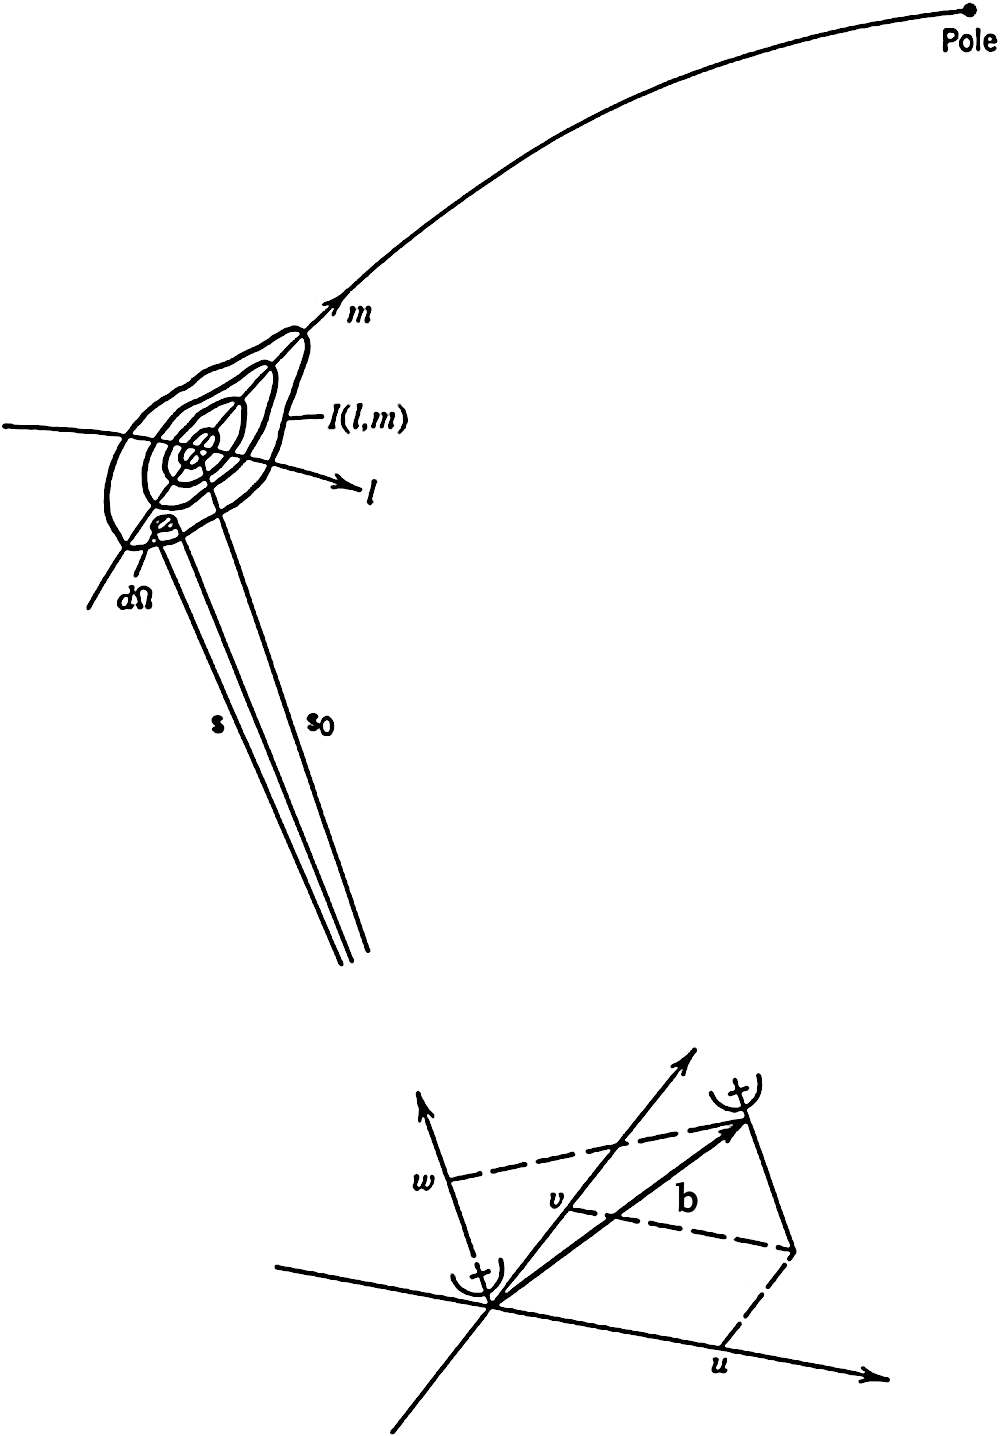
\includegraphics[width=0.7\textwidth]{interferometer-coordsys}
  \bicaption[干涉仪成像所用的 $(u,v,w)$ 直角坐标系]{%
    干涉仪成像所用的 $(u,v,w)$ 直角坐标系,
    其中 $w$ 轴指向参考方向 $\ac*{v-direction}_0$(通常为目标的中心),
    $u$ 轴向东,$v$ 轴向北。
    \acl*{v-baseline}可表示为 $\ac*{v-baseline} = (u,v,w) \lambda$,
    目标的亮度分布则用\acs*{dc}描述,
    即 $\ac*{I-nu}(\ac*{v-direction}) = \ac*{I-nu}(l,m)$,
    其中 $l, m$ 分别为\acl*{v-direction} \ac*{v-direction}
    对 $u, v$ 轴的投影长度。
  }{%
    The $(u,v,w)$ Cartesian coordinate system for interferometers,
    in which the $w$-axis points in the reference direction
    $\ac*{v-direction}_0$ (usually toward the source center), and
    the $u$- and $v$-axes point east and north, respectively.
    A baseline vector is represented as
    $\ac*{v-baseline} = (u,v,w) \lambda$,
    and the source brightness distribution is described as
    $\ac*{I-nu}(\ac*{v-direction}) = \ac*{I-nu}(l,m)$,
    where $l, m$ are direction cosines,
    i.e., the projected lengths of the direction vector \ac*{v-direction}
    against the $u$- and $v$-axes, respectively.
    \\来源/Credit:
    \citeay{thompson2017}, \S\,3.1
  }
  \label{fig:interferometer-coordsys}
\end{figure}

为了能够实际地运用\autoref{eq:vis} 从观测的\ac{vis}数据获得辐射源的亮度分布,
需要定义一个合适的坐标系。
如\autoref{fig:interferometer-coordsys} 所示的 $(u,v,w)$ 直角坐标系是最常用的,
其中 $w$ 轴指向参考方向 $\ac{v-direction}_0$(通常为目标的中心),
$u$ 轴向东,$v$ 轴向北。
于是\acl{v-baseline}为 $\ac{v-baseline} = (u,v,w) \lambda$,
\acl{v-direction}为 $\ac{v-direction} = \left( l, m, \sqrt{1-l^2-m^2} \right)$,
其中 $l$ 和 $m$ 分别为 \ac{v-direction} 对 $u$ 轴和 $v$ 轴的投影长度,即\ac{dc}。
再利用 $\D{\Omega} = \D{l}\,\D{m} \,\big/ \sqrt{1-l^2-m^2}$,
干涉仪测量的\ac{vis} [\autoref{eq:vis}] 便可表示为:
\begin{equation}
  \label{eq:vis-uvw}
  \acs{Vis}(u,v,w) = \iint \frac{\ac{I-nu}(l,m)}{\sqrt{1-l^2-m^2}}
    \exp \left[ -2\Cpi\Ci \left( ul+vm+w\sqrt{1-l^2-m^2} \right) \right]
    \,\D{l}\,\D{m} .
\end{equation}
注意,因为上式的相位因子存在额外项 \enquote{$w \sqrt{1-l^2-m^2}$},
所以这\emph{不是}二维 Fourier 变换。
但是在下述两种常见的特殊情况下,上式可变成二维 Fourier 变换,
从而可以通过逆 Fourier 变换获得目标的亮度分布 $\ac{I-nu}(l,m)$。
\begin{itemize}
\item
\emph{所有\acl{v-baseline}共面:}
这里可以进一步分为两种情形:
(1) 干涉阵列的天线只沿东西方向分布,如 \ac{wsrt} \cite{hogbom1974wsrt},
尽管地球自转,所有\acl{v-baseline}均落在同一个垂直于地球自转轴的平面内;
(2) 虽然干涉阵列的天线分布在一个二维平面,如 \ac{miteor} \cite{zheng2014},
但是采用\ac{snapshot}观测模式,即每次观测或成像的\ac{t-int}足够短。
在这两种情况下,可以选取合适的坐标系原点使得 $w = 0$,
于是\autoref{eq:vis-uvw} 变成二维 Fourier 变换,
通过逆变换可得目标的亮度分布 $\ac{I-nu}(l,m)$:
\begin{equation}
  \label{eq:vis-inv1}
  \frac{\ac{I-nu}(l,m)}{\sqrt{1-l^2-m^2}}
    = \iint \acs{Vis}(u,v, w \equiv 0)
      \exp [2\Cpi\Ci\, (ul+vm)] \,\D{u}\,\D{v} .
\end{equation}

%.......................................
\item
\emph{小视场成像:}
对于任何干涉阵列,如果只观测以参考方向 $\ac{v-direction}_0$
为中心的一个足够小的视场区域,则有:
\begin{equation}
  w \sqrt{1-l^2-m^2}
    \approx w \left[ 1 - \frac{l^2+m^2}{2} \right] .
\end{equation}
于是\autoref{eq:vis-uvw} 成为:
\begin{multline}
  \acs{Vis}(u,v,w) \approx \exp (-2\Cpi\Ci\,w) \\
    \times \iint\! \frac{\ac{I-nu}(l,m)}{\sqrt{1-l^2-m^2}}
    \exp [-2\Cpi\Ci\, (ul+vm) -\Ci\Cpi w(l^2+m^2)] \,\D{l}\,\D{m} .
\end{multline}
如果 $\big| \Cpi w(l^2+m^2) \big| \ll 1$,
即有 $\exp [-\Ci\Cpi w(l^2+m^2)] \approx 1$,
则上式变成二维 Fourier 变换,即:
\begin{align}
  \acs{Vis}(u,v)
    & \equiv \acs{Vis}(u,v,w) \exp (2\Cpi\Ci\,w)  \\
    & = \iint \frac{\ac{I-nu}(l,m)}{\sqrt{1-l^2-m^2}}
    \exp [-2\Cpi\Ci\, (ul+vm)] \,\D{l}\,\D{m} ,
  \label{eq:vis-uv}
\end{align}
然后通过逆 Fourier 变换,便得到目标的亮度分布 $\ac{I-nu}(l,m)$:
\begin{equation}
  \label{eq:vis-inv2}
  \frac{\ac{I-nu}(l,m)}{\sqrt{1-l^2-m^2}}
    = \iint \acs{Vis}(u,v)
      \exp [2\Cpi\Ci\, (ul+vm)] \,\D{u}\,\D{v} .
\end{equation}

\end{itemize}

上述第一种情况要求\acl{v-baseline} \ac{v-baseline} 全部在同一平面内,
第二种情况要求\acl{v-direction} \ac{v-direction}
在天球上的对应点全部在同一平面内,即视场足够小。
从\autoref{eq:vis} 容易看出 \ac{v-baseline} 和 \ac{v-direction} 之间存在对称性,
因此这两种情况可理解为相同近似条件的不同表现形式 \cite{clark1999}。
如果无法满足以上两种情况(比如呈三维空间分布的干涉阵列的大视场成像),
则需要采用专门的成像方法 \cite{cornwell1992,sault2007},
例如 \ac{w-proj}法 \cite{cornwell2008}、
\ac{w-stack}法 \cite{humphreys2011}
(将在 \autoref{sec:obs-simu} 使用的 \texttt{WSClean} 成像软件实现了该方法
\cite{offringa2014,offringa2017})。

%---------------------------------------------------------------------
\subsection{\texorpdfstring{$uv$}{uv} 覆盖和脏图}
\label{sec:uv-coverage}

设二元干涉仪的\acl{v-baseline}为 $\ac{v-baseline} = (u,v,w)\lambda$,
干涉仪在每个时刻测量 $uv$ 平面内位于 $(u,v)$ 和 $(-u,-v)$ 的一对\ac{vis}。
\ac{v-baseline} 的各个分量随地球自转而逐渐变化,
于是该基线在 \SI{24}{\hour} 内测量的\ac{vis}数据在 $uv$ 平面内形成两个相互对称的椭圆。
一个包含 \ac{N-ant} 个天线的干涉阵列可形成
$\ac{N-ant}(\ac{N-ant}-1)/2$ 条基线,
每条基线都可以测量 $uv$ 平面内相应位置的\ac{vis},
于是显著地增加了 $uv$ 覆盖度,即 $uv$ 平面内被测量到的范围。
\autoref{fig:uv-coverages} 展示了不同天线数目、不同\ac{t-int}的 $uv$ 覆盖。

\begin{figure}[htp]
  \centering
  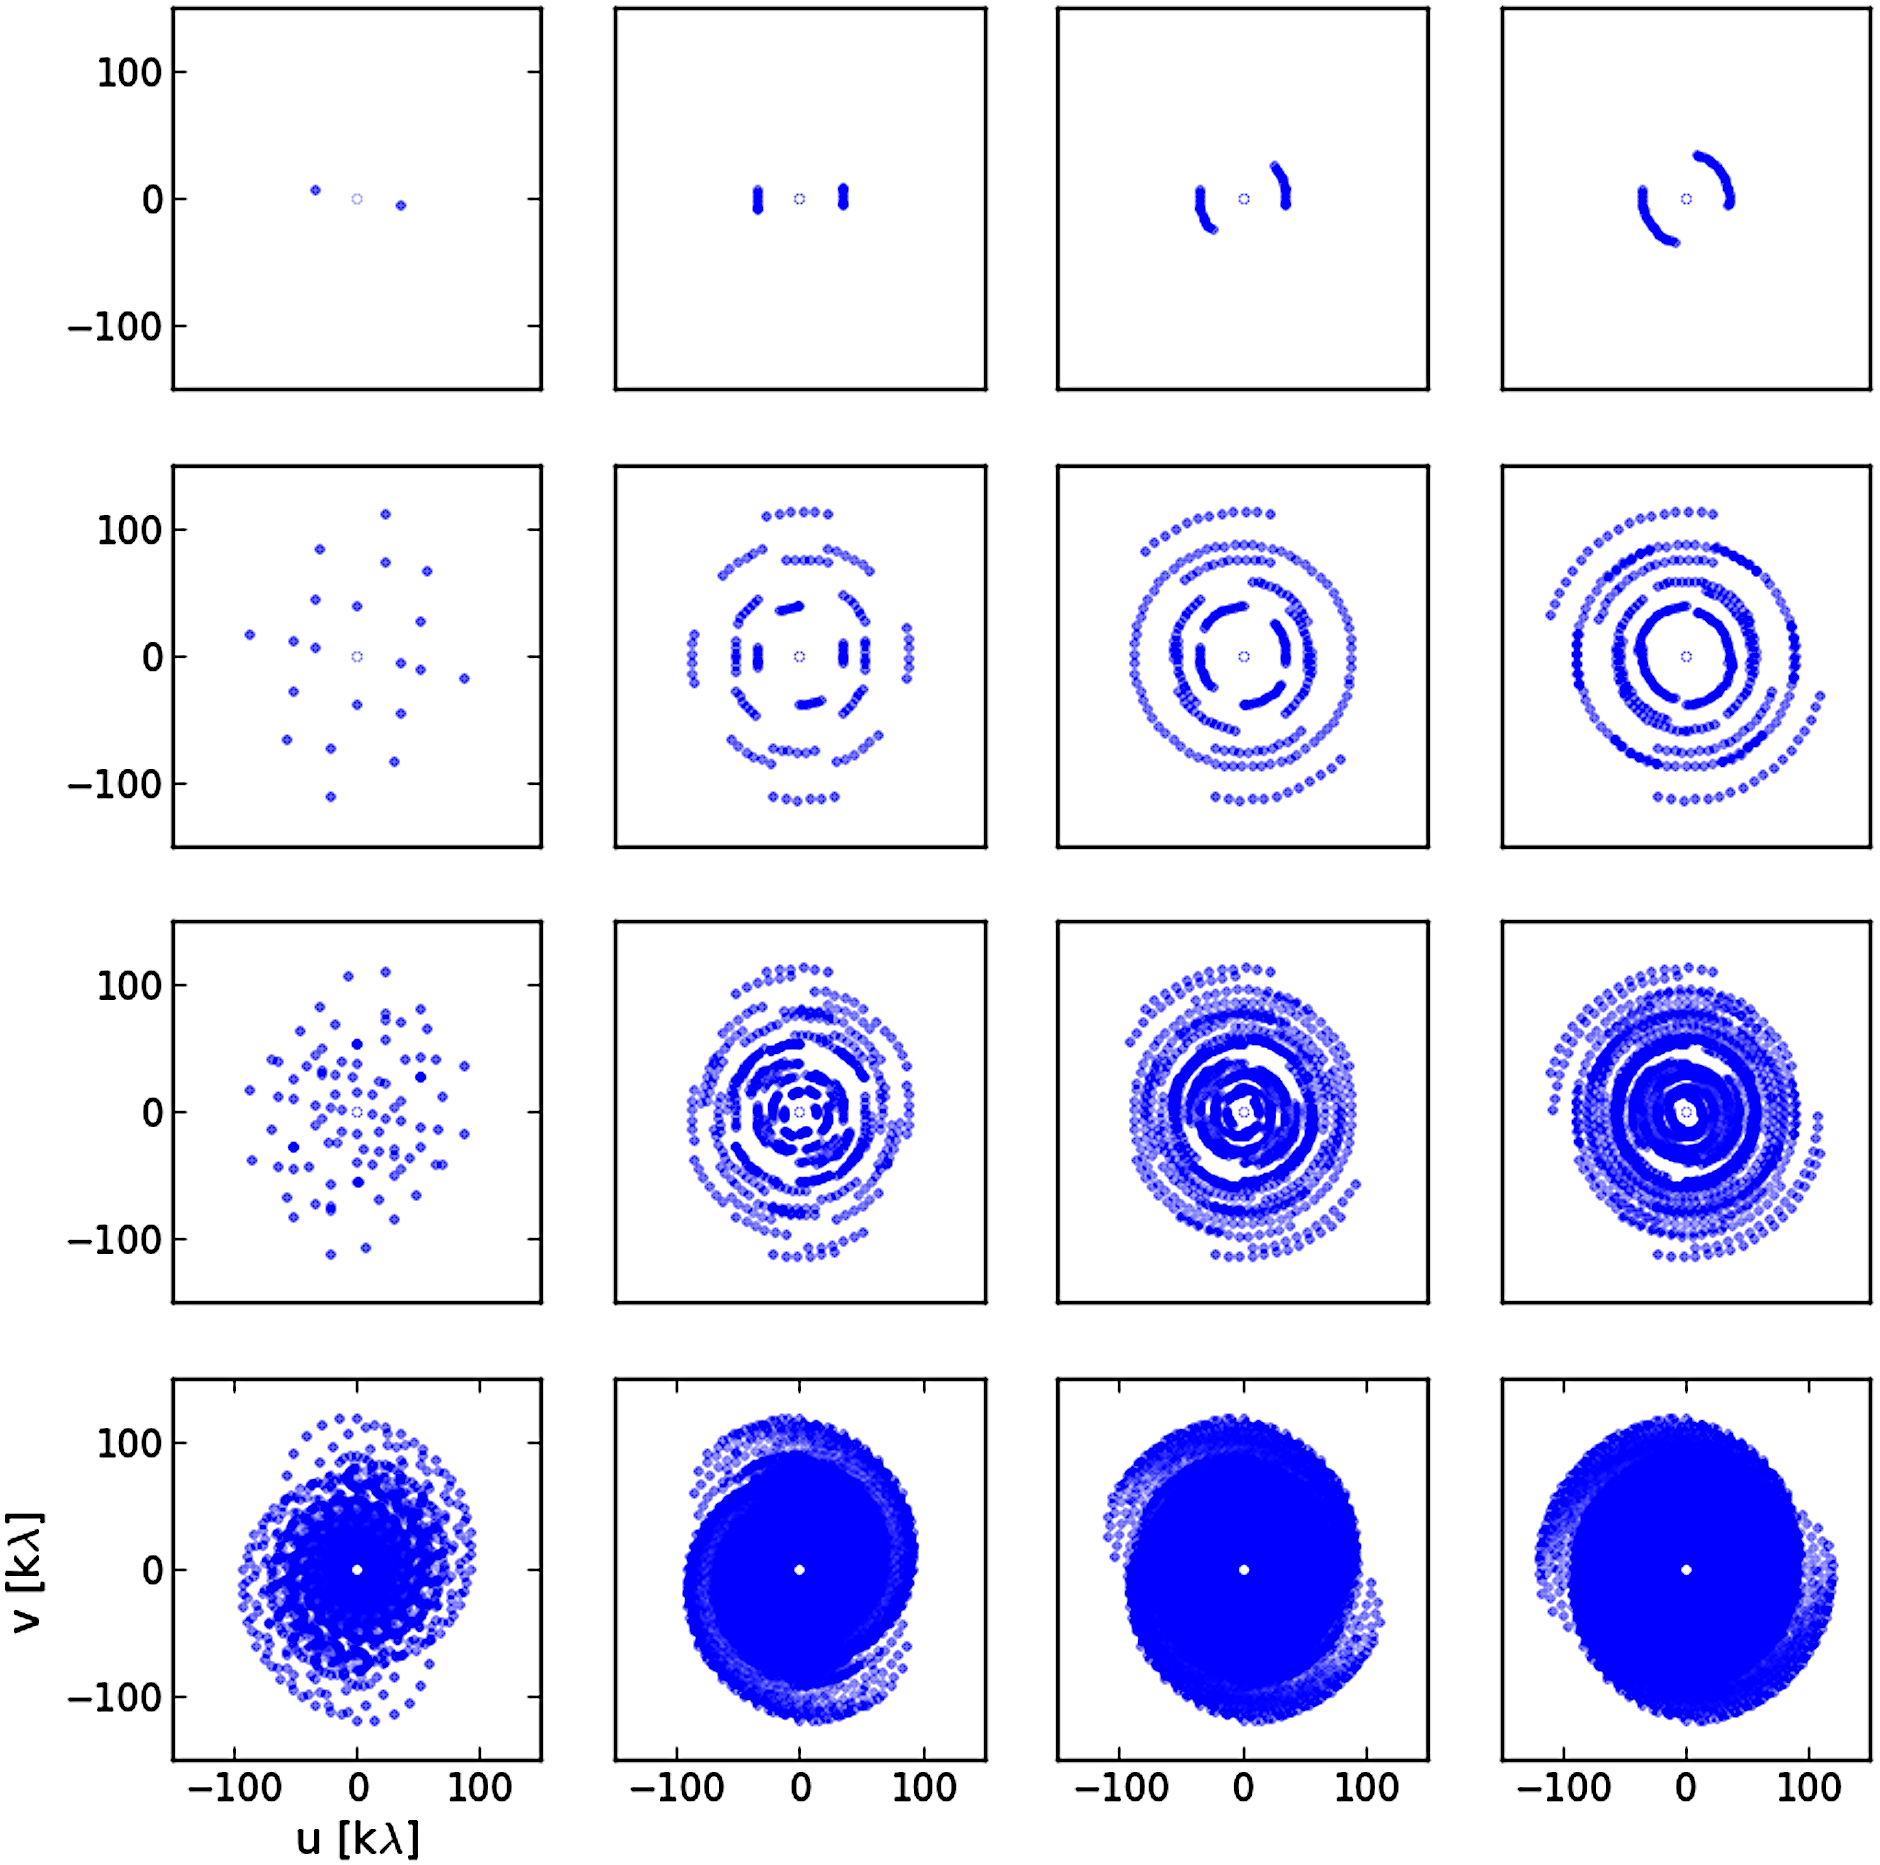
\includegraphics[width=\textwidth]{uv-coverages}
  \bicaption[不同天线数目、不同积分时间的 $uv$ 覆盖示例]{%
    不同天线数目、不同积分时间的 $uv$ 覆盖示例。
    \uline{从上往下}: 干涉阵列分别包含 2、5、10 和 50 个呈对数螺旋状分布的天线;
    \uline{从左到右}: \ac{t-int}分别为 \SI{10}{\second}、\SI{2}{\hour}、
    \SI{4}{\hour} 和 \SI{6}{\hour}。
  }{%
    Examples of $uv$ coverages.
    \uline{Top to bottom}: the interferometer includes 2, 5, 10, and 50
    antennas in a logarithmic spiral pattern, respectively;
    \uline{Left to right}: the integration time is \SI{10}{\second},
    \SI{2}{\hour}, \SI{4}{\hour}, and \SI{6}{\hour}, respectively.
    \\来源/Credit:
    \citeay{avison2013}
  }
  \label{fig:uv-coverages}
\end{figure}

因为干涉阵列的天线数目是有限的,基线的长度范围也是有限的,
所以在实际观测中 $uv$ 平面不可能被完全覆盖,
具体覆盖情况可由\acf{f-sampling}描述:
\begin{equation}
  \label{eq:sf}
  \acs{S-uv} = \sum_{k,t} \delta(u - u_{k,t}, v - v_{k,t}) ,
\end{equation}
其中 $u_{k,t}$ 和 $v_{k,t}$ 为时刻 $t$ 时基线 $\B{b}_k$ 在 $uv$ 平面内的分量。
于是,干涉阵列实际测量的\ac{vis}数据为 $\acs{Vis}(u,v) \acs{S-uv}$。
由于无法获得目标亮度分布的全部信息,
根据\autoref{eq:vis-inv2} 对测量的\ac{vis}数据进行逆 Fourier 变换
仅能得到目标的\acf{dirty-map} $I_{\nu}^D(l,m)$:
\begin{equation}
  \label{eq:dirty-map}
  \frac{I_{\nu}^D(l,m)}{\sqrt{1-l^2-m^2}} = \iint
    \acs{Vis}(u,v) \acs{S-uv} \exp [2\Cpi\Ci\, (ul+vm)] \,\D{l}\,\D{m} .
\end{equation}
利用\ac{conv-theorem},可将上式表示为:
\begin{equation}
  I_{\nu}^D(l,m) = \ac{I-nu}(l,m) * B(l,m) ,
\end{equation}
其中 \enquote{$*$} 表示卷积算符,
$B(l, m)$ 是\ac{f-sampling} \acs{S-uv} 的 Fourier 变换:
\begin{equation}
  \label{eq:syn-beam}
  B(l,m) = \iint \acs{S-uv} \exp [2\Cpi\Ci\, (ul+vm)] \,\D{l}\,\D{m} ,
\end{equation}
称为\acf{beam-synthesized}或\acf{psf}。
\autoref{fig:imaging-relations} 展示了成像过程中的主要变换关系。
为了从\ac{dirty-map} $I_{\nu}^D(l,m)$ 尽可能地恢复目标的真实图像 $\ac{I-nu}(l,m)$,
则需要使用复杂的非线性\ac{deconv}方法,
比如 CLEAN 算法 \cite{hogbom1974,cornwell1999}、
\ac{mem} \cite{narayan1986}。

\begin{figure}[htp]
  \centering
  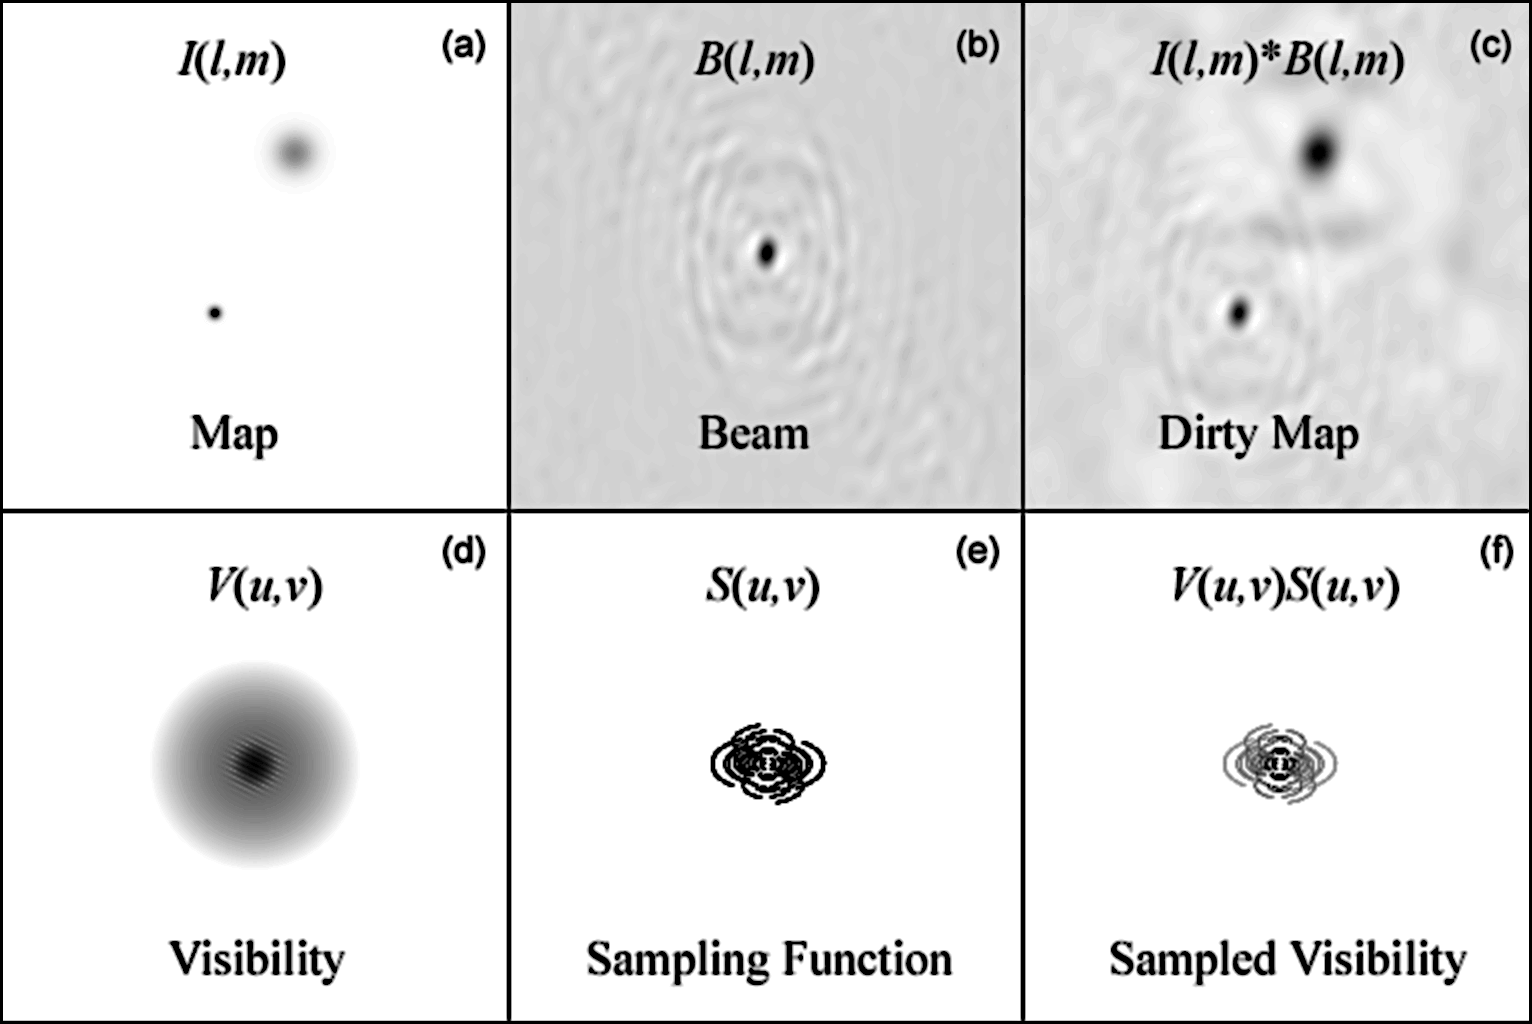
\includegraphics[width=\textwidth]{imaging-relations}
  \bicaption[干涉成像过程中的变换关系]{%
    干涉成像过程中的变换关系。
    \emph{(a)} 真实天图;
    \emph{(b)} \acs*{beam-synthesized};
    \emph{(c)} 脏图;
    \emph{(d)} 真实的\acs*{vis}数据;
    \emph{(e)} \acs*{f-sampling};
    \emph{(f)} 实际测量的\acs*{vis}数据。
    每列的两张图像互为 Fourier 变换。
  }{%
    The transform relations among the imaging process.
    \emph{(a)} True sky map;
    \emph{(b)} Synthesized beam;
    \emph{(c)} Dirty map;
    \emph{(d)} True visibility data;
    \emph{(e)} Sampling function;
    \emph{(f)} Actually measured visibility data.
    The two images in each column are the Fourier transform of each other.
    \\来源/Credit:
    Dale E. Gary, Radio Astronomy, Lecture 6,
    \url{https://web.njit.edu/~gary/728/Lecture6.html}, (2018-11-21)
    [反转了颜色]
  }
  \label{fig:imaging-relations}
\end{figure}

%---------------------------------------------------------------------
%\subsection{CLEAN 算法和洁图}
%
% TODO...

%---------------------------------------------------------------------
\subsection{点源灵敏度和亮度灵敏度}

天线的输出信号会因为自身的热噪声而存在一定的误差。
若天线的温度为 \ac{T-antenna} [参见\autoref{eq:t-ant}],
则每个时刻天线的测量值的\ac{rms}误差为
$\sigma_1 \approx \sqrt{2} \ac{T-antenna}$
(详见 \citeay{condon2016}, 附录 B.6)。
设信号的带宽为 $\Delta\nu$,根据\cite{sampling-theorem},
在时间 $\tau$ 内应采样 $N \gtrsim 2 \Delta\nu \,\tau$ 个数据点。
于是天线的测量值经过时间平均后的误差为:
\begin{equation}
  \label{eq:radiometer}
  \sigma_{\tau}
    = \frac{\sqrt{2} \ac{T-antenna}}{\sqrt{N}}
    \approx \frac{\ac{T-antenna}}{\sqrt{\Delta\nu \,\tau}} ,
\end{equation}
其中 $\tau$ 为\ac{t-int}。
\ac{t-int}越长,测量值的误差就越小,观测所达到的灵敏度就越高。
然而在实际情况中,多种系统误差会限制灵敏度的提高,
比如天线和接收机的\ac{gain}变化、大气层辐射的不规则涨落、
未分辨背景源所产生的\ac{confusion}、等等。

若一个无偏振点源的辐射使天线的温度 \ac{T-antenna} 升高了 $\Delta\ac{T-antenna}$,
则根据\autoref{eq:dt-source} 可测得该点源的流量密度为:
\begin{equation}
  S_{\nu} = \frac{2\,\ac{kb} \Delta\ac{T-antenna}}{\ac{area-eff}} ,
\end{equation}
相应的测量误差为:
\begin{align}
  \sigma_S
    & = \frac{2\,\ac{kb}}{\ac{area-eff}}
        \sigma(\ac{T-antenna} + \Delta\ac{T-antenna}) \\
    & \approx \frac{2\,\ac{kb}}{\ac{area-eff}} \sigma(\ac{T-antenna}) \\
    & = \frac{2\,\ac{kb} \ac{T-antenna}}{
      \ac{area-eff} \sqrt{\Delta\nu \,\tau}} ,
\end{align}
此即单天线的点源灵敏度。

对于由两个相同天线构成的二元干涉仪,其点源灵敏度为:
\begin{equation}
  \sigma_S
    = \frac{\sqrt{2}\,\ac{kb} \ac{T-antenna}}{
        \ac{area-eff} \sqrt{\Delta\nu \,\tau}} .
\end{equation}
由 \ac{N-ant} 个相同天线构成的干涉阵列可形成 $\ac{N-ant}(\ac{N-ant}-1)/2$
个独立的二元干涉仪,因此其点源灵敏度 $\sigma_S$ 为:
\begin{equation}
  \label{eq:sigma-ps}
  \sigma_S
    = \frac{2\,\ac{kb} \ac{T-antenna}}{
        \ac{area-eff} \sqrt{\ac{N-ant}(\ac{N-ant}-1) \Delta\nu \,\tau}} .
\end{equation}

如果观测一个\ac{src-extended},则需要考虑干涉仪的亮度灵敏度 $\sigma_b$,
可利用 Rayleigh--Jeans 近似 [\autoref{eq:rj-approx}]
直接由 $\sigma_S$ 导出:
\begin{equation}
  \label{eq:sigma-tb}
  \sigma_b = \frac{\lambda^2}{2\,\ac{kb}} \frac{\sigma_S}{\Omega_s} ,
\end{equation}
其中 $\Omega_s$ 是干涉阵列的\ac{beam-synthesized}的立体角。
相比单口径望远镜,干涉仪的基线长、角分辨率高,
所以\ac{beam-synthesized}的立体角 $\Omega_s$ 非常小。
即使干涉阵列包含许多天线,但其亮度灵敏度 $\sigma_b$
与单口径望远镜相比并不具备优势。


%% EOF

%%
%% Copyright (c) 2018-2019 Weitian LI <liweitianux@sjtu.edu.cn>
%% Creative Commons BY 4.0
%%

\acuse{2d,3d}

\chapter{再电离时期的探测}
\label{chap:detection}


\emph{\acf{eor}}是早期宇宙的一段缺乏足够了解的时期,
目前的理论研究以及有限的观测证据表明该时期从宇宙大爆炸之后约 \SI{300}{\Myr}
持续到约 \SI{1}{\Gyr},
对应红移范围约为 \numrange{6}{15}
(参见 \citeay{koopmans2015} 及其所引文献).
充分探明并理解该时期,是进一步揭示更早的\ac{cd}和\ac{da}($z > 15$)、
建立完整的宇宙演化图景的关键环节.
在低频射电波段($\sim$\,\SIrange{50}{200}{\MHz})
探测源自再电离时期的 21\,cm 信号(即\emph{EoR 信号})
是目前研究该时期的最直接而有效的办法 \cite{madau1997,tozzi2000,furlanetto2006}.


%=====================================================================
\section{EoR 信号}
\label{sec:eor-signal}

%---------------------------------------------------------------------
\subsection{21\texorpdfstring{\,}{ }cm~谱线}
\label{sec:21cm-line}

中性氢原子的原子核(即质子)和电子均有 1/2 \ac{spin},
因此均具有相应的内禀\ac{mag-moment}:
\begin{align}
  \B{\mu}_p & = |g_p| \frac{\acs{magneton-n}}{\acs{h-bar}} \B{S}_p , \\
  \B{\mu}_e & = - |g_e| \frac{\acs{magneton-b}}{\acs{h-bar}} \B{S}_e ,
\end{align}
% XXX: 'align' environment causes acro symbols not been printed in the list...
\acuse{h-bar,magneton-b,magneton-n}
其中
\ac{h-bar} 为\acl{h-bar},
$\ac{magneton-n} = \ac{e}\,\ac{h-bar} / (2 \ac{mass-p})$ 为\acl{magneton-n},
$\ac{magneton-b} = \ac{e}\,\ac{h-bar} / (2 \ac{mass-e})$ 为 \acl{magneton-b},
\ac{mass-p} 和 \ac{mass-e} 分别是质子和电子的质量,
$g_p$ 和 $g_e$ 分别为质子和电子的 $g$ 因子,
$\B{S}_p$ 和 $\B{S}_e$ 分别为质子和电子的\ac{spin}.
电子带负电,所以磁矩方向与其自旋方向相反.

\begin{figure}[htp]
  \centering
  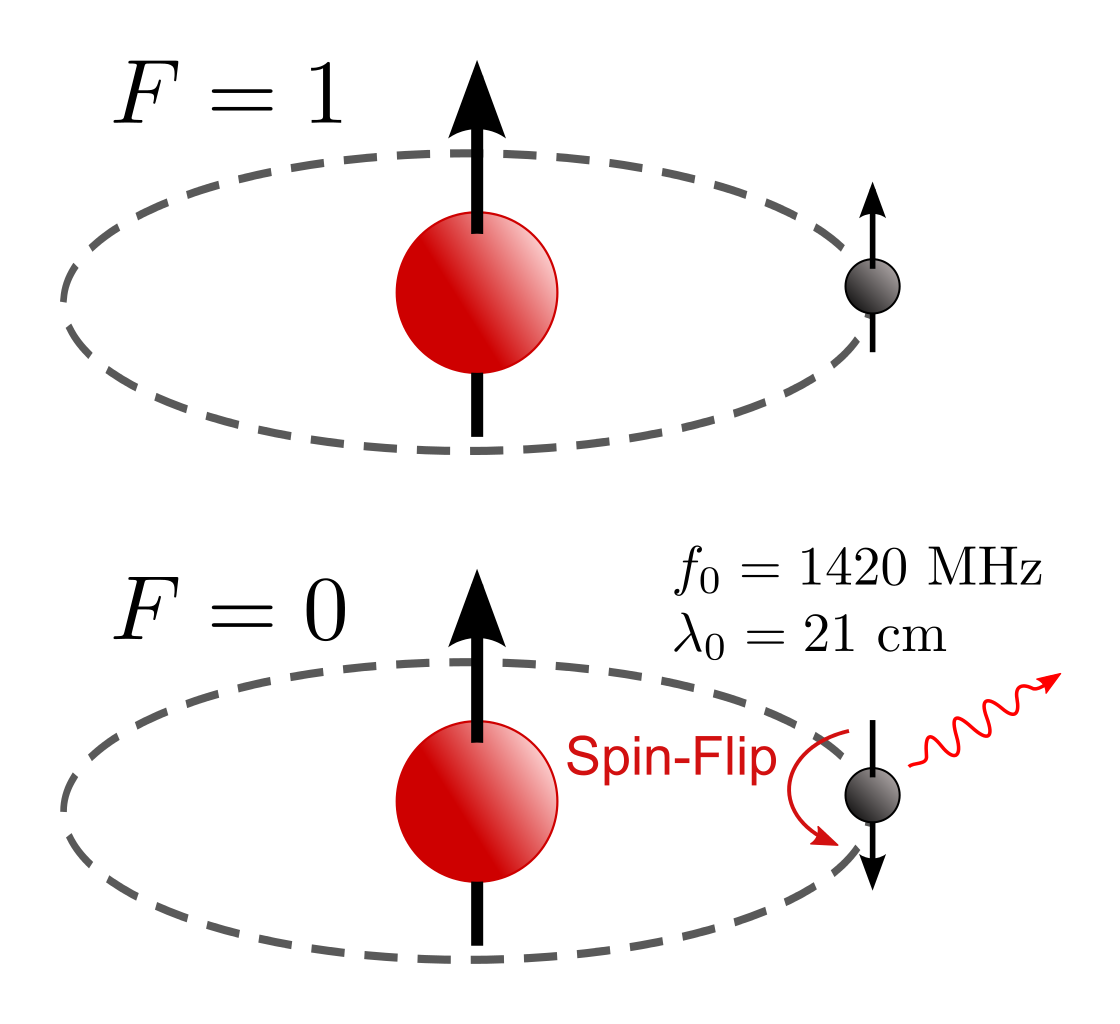
\includegraphics[width=0.5\textwidth]{hydrogen-spinflip}
  \bicaption[氢原子的自旋翻转跃迁]{%
    氢原子在基态的两个超精细分裂能级之间发生\acs*{sft},产生 \acs*{21cmline}.
  }{%
    An hydrogen atom makes a spin-flip transition between the two
    hyperfine levels of the ground state, emitting the 21\,cm line.
    \\来源/Credit:
    Tiltec,
    \url{https://en.wikipedia.org/wiki/File:Hydrogen-SpinFlip.svg},
    (2019-03-31), 公有领域.
  }
  \label{fig:hi-spinflip}
\end{figure}

因为质子和电子的自旋发生相互作用,所以氢原子的\ac{ground-state}
发生\ac{hyperfine-splitting}而变成两个态:
(1) 质子的\ac{spin} $\B{S}_p$ 和电子的\ac{spin} $\B{S}_e$ 平行,总角动量 $F = 1$;
(2) $\B{S}_p$ 和 $\B{S}_e$ 反平行,总角动量 $F = 0$.
想像两个共中心的载流线圈,系统的稳定状态(即能量最低)为两个线圈的电流方向相同,
即两个载流线圈的磁矩平行.
将此应用于上述两个态,可知 $F = 1$ 态(即质子和电子的\ac{spin}反平行、磁矩平行)
的能量比 $F = 0$ 态更高 \cite{griffiths1982}.
当氢原子从 $F = 1$ 态跃迁到 $F = 0$ 态时,
将产生频率约为 $\nu = \SI{1420}{\MHz}$ 的辐射,
对应的波长约为 $\lambda = \SI{21}{\cm}$,因此称为\emph{\acf{21cmline}}.
此跃迁过程亦称为\emph{\acf{sft}},如\autoref{fig:hi-spinflip} 所示.
对于 $F = 1$ 态(即上能级),磁量子数 $m$ 可取 $\big\{ -1, 0, 1 \big\}$,
因此这个态的\ac{dod}为 3,称为\emph{\acf{triplet}};
对于 $F = 0$ 态(即下能级),磁量子数 $m$ 只能取 0,
因此这个态是\emph{\acf{singlet}}.

中性氢的 \ac{21cmline}%
首次由 H.~C. van~de~Hulst 在 1945 年提出 \cite{vanDeHulst1945},
并由 H.~I. Ewen 和 E.~M. Purcell 在 1951 年观测到 \cite{ewen1951}.
该谱线的频率 \ac{freq21cm} 是目前测量最精确的几个物理量之一
\cite{hellwig1970,essen1971}:
\begin{equation}
  \label{eq:hi-line-frequency}
  \acs{freq21cm} = \SI{1420405751.7667 +- 0.0009}{\Hz} ,
\end{equation}
对应真空中的波长为:
\begin{equation}
  \label{eq:hi-line-wavelength}
  \lambda_0 = \SI{21.1061140542}{\cm} .
\end{equation}

%---------------------------------------------------------------------
\subsection{谱线亮温度}

中性氢的 \ac{21cmline}的跃迁概率非常低,其\acl{coef-A21} \ac{coef-A21} 为:
\begin{equation}
  \ac{coef-A21} =
    \SI[separate-uncertainty=false]{2.86888(7)e-15}{\per\second} .
\end{equation}
对应的\ac{em-spontaneous}的半衰期为:
\begin{equation}
  t_{1/2} \approx 1 / \ac{coef-A21}
    = \SI{3.49e14}{\second} \approx \SI{11.1}{\Myr} .
\end{equation}
该\ac{timescale}远大于典型中性氢云中的氢原子因碰撞而改变\ac{spin}的\ac{timescale},
因此中性氢的超精细结构的能级布居将由碰撞决定.

由\autoref{eq:t-excitation-def}可知,\acl{T-excitation}描述了能级的相对布居.
鉴于 \ac{21cmline}源自中性氢的\ac{sft},在此情况下,
\acl{T-excitation}亦被称为\emph{\acl{T-spin} (spin temperature)} \ac{T-spin},
描述了氢原子自旋态(即\ac{singlet}和\ac{triplet})的相对布居 \cite{field1958}:
\begin{equation}
  \frac{N_2}{N_1} = \frac{g_2}{g_1}
    \exp\left( -\frac{\acs{hp} \nu_0}{\acs{kb} \acs{T-spin}} \right)
    = \frac{g_2}{g_1} \exp\left( -\frac{T_*}{\acs{T-spin}} \right),
\end{equation}
其中
$g_1 = 1$ 和 $g_2 = 3$ 分别为两个能级的\ac{dod},
$T_* \equiv \acs{hp} \nu_0 / \acs{kb} \approx \SI{68.2}{\mK}$.
在实际的天体物理应用中,均有 $\acs{T-spin} \gg T_*$,因此:
\begin{equation}
  \frac{N_2}{N_1} = \frac{g_2}{g_1} = 3 .
\end{equation}
将此代入\autoref{eq:coef-absorption-einstein3},
近似后可得中性氢云的\acl{coef-absorption}为:
\begin{equation}
  \acs{coef-absorption}
    = \frac{3 \acs{hp} \acs{speed-light}^2}{32\Cpi \nu_0}
      \frac{A_{21} n_{\R{HI}}}{\acs{kb} \acs{T-spin}} \phi(\nu) ,
\end{equation}
其中 $n_{\R{HI}} = N_1 + N_2 = 4 N_1$ 为中性氢的数密度.

设一团均匀的中性氢云位于红移 $z$ 处,沿视线方向的长度为 $s$,
中性氢的数密度为 $n_{\R{HI}}$,
则其\acl{optical-depth} [\autoref{eq:optical-depth}] 为:
\begin{align}
  \acs{optical-depth}_{\nu_0}
    & = \int_{\R{cloud}} \acs{coef-absorption}(s') \,\D{s'}  \\
    & = \frac{3 \acs{hp} \acs{speed-light}^2}{32\Cpi \nu_0}
      \frac{A_{21}}{\acs{kb} \acs{T-spin}} \phi(\nu)
      \int_{\R{cloud}} n_{\R{HI}}(s') \,\D{s'}  \\
    & = \frac{3 \acs{hp} \acs{speed-light}^2}{32\Cpi \nu_0}
      \frac{A_{21}}{\acs{kb} \acs{T-spin}} N_{\R{HI}} \phi(\nu) ,
  \label{eq:21cm-optical-depth1}
\end{align}
其中 $N_{\R{HI}}$ 为中性氢的\ac{column-density},可进一步写成:
\begin{equation}
  \label{eq:column-density}
  N_{\R{HI}} = s \, n_{\R{HI}} \acs{hi-fraction} ,
\end{equation}
其中 \acs{hi-fraction} 为\acl{hi-fraction} (neutral fraction of hydrogen).

一般而言,\ac{line-profile}与自然展宽 (natural broadening)、
热展宽 (thermal broadening)、压力展宽 (pressue broadening)、
体运动展宽 (bulk motion broadening) 等多种因素相关.
但是对于 \ac{21cmline},最重要的展宽因素是宇宙膨胀引起的 Doppler 展宽.
根据 Hubble 定律,线性尺度为 $s$ 的中性氢云的速度弥散约为
$\Delta v \sim s \acs{Hz}$,
于是\ac{line-profile}可近似为 \cite{furlanetto2006,morales2010}:
\begin{equation}
  \phi(\nu) \sim \frac{\acs{speed-light}}{\nu \Delta v}
    \sim \frac{\acs{speed-light}}{\nu \, s \acs{Hz}} .
\end{equation}
将上式和\autoref{eq:column-density} 代入\autoref{eq:21cm-optical-depth1},
可得\acl{optical-depth}:
\begin{equation}
  \label{eq:21cm-optical-depth2}
  \acs{optical-depth}_{\nu_0}
    \approx \frac{3 \acs{hp} \acs{speed-light}^3}{32\Cpi \nu_0^2}
      \frac{A_{21}}{\acs{kb} \acs{T-spin}}
      \frac{\acs{hi-fraction} n_{\R{HI}}}{\acs{Hz}} .
\end{equation}
如果需要考虑中性氢云的\ac{v-peculiar},则其\acl{optical-depth}应为
\cite{bharadwaj2005,furlanetto2006,pritchard2012}:
\begin{equation}
  \label{eq:21cm-optical-depth3}
  \acs{optical-depth}_{\nu_0}
    \approx \frac{3 \acs{hp} \acs{speed-light}^3}{32\Cpi \nu_0^2}
      \frac{A_{21}}{\acs{kb} \acs{T-spin}}
      \frac{\acs{hi-fraction} n_{\R{HI}}}{
        (1+z) (\partial v_{\parallel} / \partial r_{\parallel})} ,
\end{equation}
其中 $(\partial v_{\parallel} / \partial r_{\parallel})$ 是\ac{v-proper}
沿视线方向的梯度.
此外,中性氢云的\acl{optical-depth} 通常满足
$\acs{optical-depth}_{\nu0} \ll 1$
\cite{madau1997,furlanetto2006,pritchard2010mn}.

\begin{figure}[htp]
  \centering
  
\includegraphics[width=0.9\textwidth]{21cm-radiative-transfer}
  \bicaption[CMB 辐射穿过中性氢云的辐射转移示意图]{%
    CMB 辐射穿过中性氢云的辐射转移示意图:
    从\acl*{T-spin}为 \acs*{T-spin} 的中性氢云出射的
    CMB 辐射的温度为 \acs*{T-b}.
  }{%
    An illustration of the radiative transfer process:
    the CMB radiation goes through a cloud of hydrogen with
    spin temperature \acs*{T-spin} and emerges with a temperature
    \acs*{T-b} measured by a telescope.
    \\来源/Credit:
    \citeay{zaroubi2013}, \S\,4.1.
    [经过了左右翻转]
  }
  \label{fig:21cm-cmb-rt}
\end{figure}

在实际观测中,需要考虑 \ac{cmb} 辐射穿过中性氢云的转移过程,
如\autoref{fig:21cm-cmb-rt} 所示.
考虑一团处于热平衡状态、\acl{T-spin}为 \acs{T-spin}、位于红移 $z$ 处的中性氢云,
结合 Kirchhoff 定律 [\autoref{eq:kirchhoff-law}] 可得\ac{rt}方程为:
\begin{equation}
  \diff{\acs{I-nu}}{s}
    = -\acs{coef-absorption}\,\acs{I-nu} + \acs{coef-emission}
    = -\acs{coef-absorption}\,[\acs{I-nu} - B_{\nu}(\acs{T-spin})] ,
\end{equation}
其中
$B_{\nu}(\acs{T-spin})$ 是温度为 \acs{T-spin} 的黑体辐射谱 [\autoref{eq:planck}].
利用 Rayleigh--Jeans 近似 [\autoref{eq:rj-approx}]
可将 \acs{I-nu} 表示为\acl{T-b} $\acs{T-b}(\nu)$,于是有:
\begin{equation}
  \diff{\acs{T-b}}{s}
    = -\acs{coef-absorption} [\acs{T-b} - \acs{T-spin}] .
\end{equation}
根据\acl{optical-depth}的定义 [\autoref{eq:optical-depth}]
有 $\D{\tau'} = -\acs{coef-absorption}\,\D{s}$,
代入上式可得:
\begin{equation}
  \diff{\acs{T-b}}{\tau'} = \acs{T-b} - \acs{T-spin} .
\end{equation}
在上式两边均乘上 $\Ce^{-\tau'}\,\D{\tau'}$ 并积分:
\begin{equation}
  \acs{T-b}\,\Ce^{-\tau'}\,\Big|_0^{\tau_{\nu_0}}
      - \int_0^{\tau_{\nu_0}} \acs{T-b}\,\D{(\Ce^{-\tau'})}
    = \int_0^{\tau_{\nu_0}} \acs{T-b}\,\Ce^{-\tau'}\,\D{\tau'}
      + \acs{T-spin} \int_0^{\tau_{\nu_0}} \Ce^{-\tau'}\,\D{\tau'} ,
\end{equation}
可得:
\begin{equation}
  \acs{T-b}(\tau'=\tau_{\nu_0})\,\Ce^{-\tau_{\nu}} - \acs{T-b}(\tau'=0)
    = \acs{T-spin} (\Ce^{-\tau_{\nu}} - 1) ,
\end{equation}
其中 $\acs{T-b}(\tau'=\tau_{\nu_0}) = T_{\R{cmb}}(z)$
为辐射入射中性氢云时的亮温度,
于是获得从中性氢云出射 ($\tau = 0$) 的辐射亮温度 $\acs{T-b}(\nu_0)$ 为:
\begin{equation}
  \acs{T-b}(\nu_0)
    = \acs{T-spin} (1 - \Ce^{-\tau_{\nu_0}})
      + T_{\R{cmb}}(z) \,\Ce^{-\tau_{\nu_0}} .
\end{equation}
其中 $T_{\R{cmb}}(z)$ 为 \ac{cmb} 辐射在红移 $z$ 时的\ac{comoving-frame}
中的亮温度:
\begin{align}
  T_{\R{cmb}}(z)
    & = T_{\R{cmb}}(z=0)\,(1+z)  \\
    & = 2.73 \,(1+z) \quad [\si{\kelvin}] ,
\end{align}
类似地,宇宙膨胀的红移效应将中性氢 \ac{21cmline}红移至频率
$\nu = \acs{freq21cm}/(1+z)$,
同时观测到的中性氢云的亮温度将为:
\begin{equation}
  T_b^{\R{obs}}(\nu) = \frac{T_b(\acs{freq21cm})}{1 + z} .
\end{equation}
目前观测 \ac{21cmline}的策略是测量其相对于 \ac{cmb} 辐射的差异,
即\emph{\acl{dT-b} (differential brightness temperature)}.
综上,并结合\autoref{eq:21cm-optical-depth3},
得到待探测的 \emph{EoR 信号}的\acl{dT-b} \ac{dT-b} 为:
\begin{align}
  \acs{dT-b}(\nu)
    & = \frac{T_b(\acs{freq21cm})}{1 + z} - T_{\R{cmb}}(z=0)  \\
    & = \frac{\acs{T-spin} - T_{\R{cmb}}(z)}{1+z}
      (1 - \Ce^{-\acs{optical-depth}_{\nu_0}})  \\
    & \approx \frac{\acs{T-spin} - T_{\R{cmb}}(z)}{1+z}
      \acs{optical-depth}_{\nu_0}  \\
    & \approx \frac{3 \acs{hp} \acs{speed-light}^3 A_{21}}{
      32\Cpi \nu_0^2 \,\acs{kb}}
      \frac{\acs{hi-fraction} n_{\R{HI}}}{
        (1+z)^2 (\partial v_{\parallel} / \partial r_{\parallel})}
      \left[ 1 - \frac{T_{\R{cmb}}(z)}{\acs{T-spin}} \right] .
    \label{eq:eor-signal1}
\end{align}

由于再电离时期的红移较大 ($z \gtrsim 6$),
因此 Hubble 常数 [\autoref{eq:hubble-z}] 可近似为:
\begin{equation}
  \acs{Hz} = \acs{H0} \sqrt{\acs{Om0} (1+z)^3 + \acs{Ol0}}
    \approx \acs{H0} \Omega_m^{1/2} (1+z)^{3/2} .
\end{equation}
结合\autoref{eq:omega-m-z},可得红移 $z$ 时的宇宙重子物质的密度参数为:
\begin{equation}
  \acs{Ob0}(z) = \frac{\acs{Ob0}}{\acs{Om0}} \acs{Om0}(z)
    \approx \frac{\acs{Ob0}}{\acs{Om0}} .
\end{equation}
再利用当地的重子物质\ac{overdensity},即
\begin{equation}
  1 + \delta_b = \frac{\rho_b}{\overline{\rho}_b}
    \approx \frac{n_{\R{HI}} \acs{mass-p}}{\acs{Ob0}(z) \acs{rho-crit}(z)} ,
\end{equation}
其中 $\acs{rho-crit}(z)$ 为\acl{rho-crit} [\autoref{eq:rho-crit}],
可将中性氢的数密度 $n_{\R{HI}}$ 表示为:
\begin{align}
  n_{\R{HI}}
    & \approx \frac{1+\delta_b}{\acs{mass-p}} \frac{\acs{Ob0}}{\acs{Om0}}
      \frac{3 H^2(z)}{8 \Cpi \acs{G}}  \\
    & \approx \frac{3 \acs{H0}}{8\Cpi\acs{mass-p}\acs{G}}
      \frac{\acs{Ob0}}{\Omega_m^{1/2}} (1+\delta_b) (1+z)^{3/2} \acs{Hz} .
\end{align}
将上式代入\autoref{eq:eor-signal1},可得 EoR 信号的最终表达式:
\begin{align}
  \acs{dT-b}(\nu)
    & \approx \frac{9 \acs{hp} \acs{speed-light}^3 A_{21}}{
      256\Cpi^2 \nu_0^2 \,\acs{kb} \acs{mass-p} \acs{G}}
      \frac{\acs{H0} \acs{Ob0}}{\Omega_m^{1/2}}
      \acs{hi-fraction} (1+\delta_b) (1+z)^{1/2}
      \left[ 1 - \frac{T_{\R{cmb}}(z)}{\acs{T-spin}} \right]
      \left[ \frac{\acs{Hz} / (1+z)}{
        \partial v_{\parallel} / \partial r_{\parallel}} \right]
  \label{eq:eor-signal2}  \\
    & \approx \left( \SI{38}{\mK} \right)
      \acs{hi-fraction} (1+\delta_b)
      \left( \frac{1+z}{10} \right)^{1/2}
      \left( \frac{0.27}{\acs{Om0}} \right)^{1/2}
      \left( \frac{\acs{Ob0} \acs{h}^2}{0.023} \right)
      \left[ 1 - \frac{T_{\R{cmb}}(z)}{\acs{T-spin}} \right]
      \left[ \frac{\acs{Hz} / (1+z)}{
        \partial v_{\parallel} / \partial r_{\parallel}} \right] .
  \label{eq:eor-signal3}
\end{align}

%---------------------------------------------------------------------
\subsection{亮温度的演化}

由\autoref{eq:eor-signal2} 易知,中性氢云的 \acl{T-spin} \acs{T-spin}
对 EoR 信号 $\acs{dT-b}(\nu)$ 的强度起关键作用.
当 $\acs{T-spin} > T_{\R{cmb}}(z)$ 时,$\acs{dT-b}(\nu) > 0$ 为发射信号,
并且当 $\acs{T-spin} \gg T_{\R{cmb}}(z)$ 时 $\acs{dT-b}(\nu)$ 达到饱和;
当 $\acs{T-spin} < T_{\R{cmb}}(z)$ 时,$\acs{dT-b}(\nu) < 0$ 表现为吸收信号.
\acl{T-spin} \acs{T-spin} 主要由以下三个过程决定 \cite{pritchard2012}:
\begin{itemize}
  \item CMB 光子被中性氢吸收或者使中性氢产生\ac{em-stimulated},
    该过程使得 \acs{T-spin} 与 $T_{\R{cmb}}(z)$ 相互耦合;
  \item 中性氢原子与其他原子或电子碰撞,
    这个过程将 \acs{T-spin} 耦合到气体的\acl{T-kinetic} \acs{T-kinetic};
  \item 中性氢原子与 Lyα 光子发生\ac{resonant-scattering}而改变自旋状态,
    即 Wouthuysen--Field 效应 \cite{wouthuysen1952,field1958},
    该过程将 \acs{T-spin} 与 Lyα 辐射的\ac{T-color}关联起来.
\end{itemize}

\begin{figure}[htp]
  \centering
  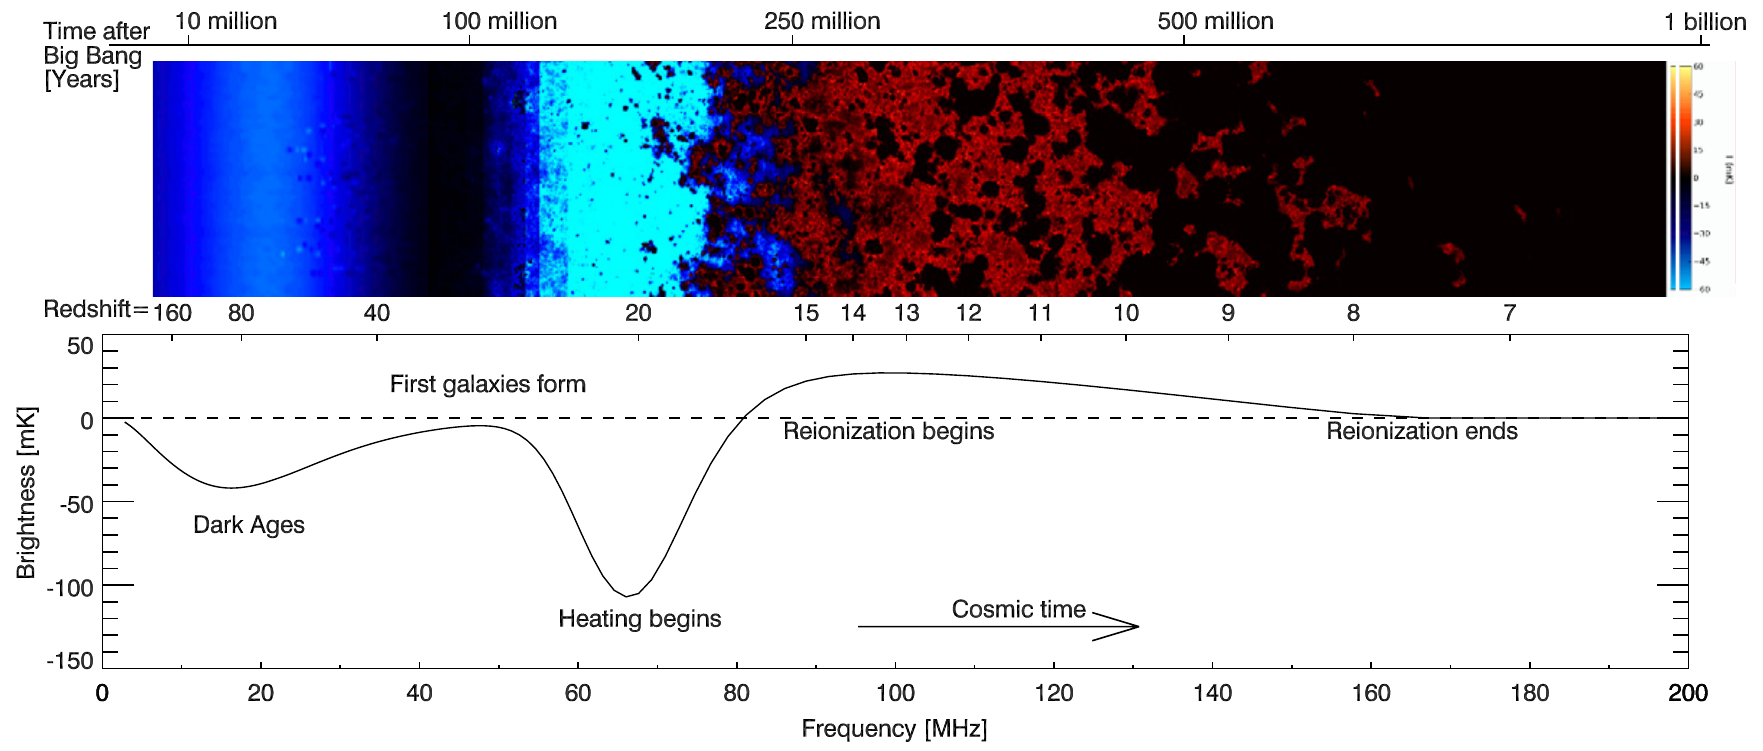
\includegraphics[width=\textwidth]{eor-signal-evolution}
  \bicaption[EoR 信号的平均强度的演化示意图]{%
    \uline{(上栏)}
    宇宙学模拟\cite{santos2008}给出的 EoR 信号的演化过程.
    \uline{(下栏)}
    理论模型给出的 EoR 信号的全天平均强度
    $\delta\overline{T}_b$ 的变化过程.
  }{%
    \emph{(Upper)} The time evolution of the EoR signal dervied from
    a cosmological simulation \cite{santos2008}.
    \emph{(Lower)} The expected evolution of the sky-averaged EoR signal
    $\delta\overline{T}_b$.
    \\来源/Credit:
    \citeay{pritchard2012}, \S\,1.
  }
  \label{fig:eor-signal-evo}
\end{figure}

上述过程与宇宙的再电离过程、第一代天体的形成、星系的形成与演化等环节密切相关,
因此 EoR 信号随宇宙的演化而发生复杂的变化,并反映在其频谱上
(不同的频率对应于不同的红移,即宇宙年龄),如\autoref{fig:eor-signal-evo} 所示.
EoR 信号的整个演化过程可大致分为以下几个阶段 \cite{pritchard2012}:
\begin{enumerate}
  \item $200 \lesssim z \lesssim 1100$:
    \ac{recombination}之后残留的自由电子通过 Compton 散射使气体
    和 \ac{cmb} 之间形成耦合,
    即有 $\acs{T-kinetic} = T_{\R{cmb}}$.
    在此阶段,因为气体的密度很高,有效的碰撞使得 $\acs{T-spin} = T_{\R{cmb}}$,
    所以此阶段没有可探测的 EoR 信号 ($\delta\overline{T}_b = 0$).

  \item $40 \lesssim z \lesssim 200$:
    气体绝热冷却从而有 $\acs{T-kinetic} < T_{\R{cmb}}$,
    但气体中的碰撞仍然足够有效,
    因此 $\acs{T-spin} = \acs{T-kinetic} < T_{\R{cmb}}$,
    所以 EoR 信号在此阶段表现为吸收信号 ($\delta\overline{T}_b < 0$).

  \item $z_* \lesssim z \lesssim 40$:
    ($z_*$ 对应第一代天体形成的时刻.)
    气体密度随着宇宙膨胀而显著降低,导致碰撞耦合不如 \ac{cmb} 辐射的耦合有效,
    因此有 $\acs{T-spin} = T_{\R{cmb}}$,所以此阶段无可探测的 EoR 信号.

  \item $z_{\alpha} \lesssim z \lesssim z_*$:
    ($z_{\alpha}$ 对应 Lyα 光子的耦合达到饱和的时刻.)
    第一代天体开始形成,辐射 Lyα 光子和 X 射线,
    从而将 \acs{T-spin} 与冷气体的温度耦合到一起,
    即 $\acs{T-spin} \sim \acs{T-kinetic} < T_{\R{cmb}}$,
    因此该阶段可探测到 EoR 吸收信号 ($\delta\overline{T}_b < 0$).

  \item $z_h \lesssim z \lesssim z_{\alpha}$:
    ($z_h$ 对应气体被加热至与 $T_{\R{cmb}}$ 相同温度的时刻.)
    随着星系和宇宙大尺度结构的形成,气体逐渐被加热,
    对 \acs{T-spin} 的影响也越来越显著.
    在气体温度 $\acs{T-kinetic} \sim \acs{T-spin} < T_{\R{cmb}}$
    的这一阶段,可继续探测到 EoR 吸收信号 ($\delta\overline{T}_b < 0$).

  \item $z_t \lesssim z \lesssim z_h$:
    随着气体被进一步加热,$\acs{T-kinetic} \sim \acs{T-spin} > T_{\R{cmb}}$,
    于是 EoR 信号从上一阶段的吸收信号转变为发射信号 ($\delta\overline{T}_b > 0$).
    直到 $z_t$ 时刻,气体的温度已经足够高
    ($\acs{T-kinetic} \sim \acs{T-spin} \gg T_{\R{cmb}}$),
    EoR 信号的强度达到饱和.

  \item $z_r \lesssim z \lesssim z_t$:
    在此阶段,气体的温度 ($\acs{T-kinetic} \sim \acs{T-spin} \gg T_{\R{cmb}}$)
    对 EoR 信号的影响已变得不重要,
    因此 EoR 信号的强度将主要取决于\acl{hi-fraction} \acs{hi-fraction}.
    随着再电离的进行,\acs{hi-fraction} 逐渐变小,EoR 信号的强度也随之减小,
    直到 $z_r$ 时再电离结束.

  \item $z \lesssim z_r$:
    再电离结束后,残留的 21\,cm 信号主要源自一些塌缩的中性氢岛,比如\ac{dla}.
\end{enumerate}

由于缺乏足够的观测证据的约束,上述阶段的划分仍有很大的不确定性,
相邻阶段之间可能有显著交叠,甚至 $z_{\alpha}$ 和 $z_h$ 的次序可能需要修正
\cite{nusser2005,pritchard2012}.
基于目前非常有限的观测证据,理论模型显示宇宙的再电离过程约从红移 $z \sim 15$ 开始,
应在红移 $z > 6.5$ 之前完成,但也不能显著早于 $z \sim \numrange{7}{8}$
\cite{choudhury2006,pritchard2010mn}.


%=====================================================================
\section{功率谱}
\label{sec:ps}

由于宇宙膨胀,位于红移 $z$ 处的中性氢云产生的 \ac{21cmline}将被红移至频率
$\nu = \acs{freq21cm} / (1 + z)$,
其中 \acs{freq21cm} 为 \ac{21cmline}的本征频率
[\autoref{eq:hi-line-frequency}].
据此,对于某一视线方向,通过在不同的频率测量 \ac{21cmline},
便可以相应地重构出中性氢在该视线上的分布情况.
对于一个天区,如果获得 \ac{21cmline}在一段频率内的图像 $I(\B{\theta},\nu)$,
即\ac{imgcube},便可以重构出中性氢的三维分布,
其中两个空间维度 $\B{\theta}$ 映射到中性氢的横向距离,
频率维度 $\nu$ 对应中性氢的视向距离.
此即 \emph{EoR \acf{tomography}} \cite{mellema2015}.

通过对 EoR 信号的\ac{imgcube} $I(\B{\theta},\nu)$ 进行三维 Fourier 变换:
\begin{equation}
  \label{eq:ft3d}
  \tilde{I}(\B{u}, \eta) =
    \int I(\B{\theta},\nu) \exp[ -2\Cpi\Ci (\B{u}\cdot\B{\theta} + \eta\nu) ]
    \,\mathrm{d}^2\B{\theta}\,\D{\nu} ,
\end{equation}
其中 $(\B{u}, \eta) = 1 / (\B{\theta}, \nu)$ 分别是
空间维度 $\B{\theta}$ 和频率维度 $\nu$ 的 Fourier \ac{dual},
可以得到由下式定义的三维\ac{ps} $P'(\B{u}, \eta)$:
\begin{equation}
  \label{eq:ps3d}
  \langle \tilde{I}(\B{u}, \eta) \, \tilde{I}^*(\B{u}', \eta') \rangle
    \equiv P'(\B{u}, \eta) \delta(\B{u}-\B{u}') \delta(\eta-\eta') ,
\end{equation}
其中 \enquote{$*$} 表示\ac{conjugate}算符.

宇宙学研究需要使用\ac{comoving-frame},
而且采用的 Fourier 约定也与射电干涉成像所采用的约定不同.
在宇宙学研究领域,
一个三维场 $T(\B{r}_{\perp}, r_{\parallel})$ 的 Fourier 变换表示为:
\begin{equation}
  \label{eq:ft3d-k}
  \tilde{T}(\B{k}_{\perp}, k_{\parallel}) =
    \int T(\B{r}_{\perp}, r_{\parallel})
    \exp[ -\Ci (\B{k}_{\perp} \cdot \B{r}_{\perp}
      + k_{\parallel} r_{\parallel}) ]
    \,\mathrm{d}^2\B{r}_{\perp} \,\D{r}_{\parallel} ,
\end{equation}
其中 $(\B{r}_{\perp}, r_{\parallel})$ 分别表示
垂直于视线方向和平行于视线方向的\acl{D-comoving},
$(\B{k}_{\perp}, k_{\parallel}) = 2\Cpi / (\B{r}_{\perp}, r_{\parallel})$
分别表示 Fourier 空间中垂直于视线方向和平行于视线方向的\ac{wavenumber}.
注意,对比\autoref{eq:ft3d},上式的相位因子少了系数 $2\Cpi$.
于是,相应的逆 Fourier 变换为:
\begin{equation}
  T(\B{r}_{\perp}, r_{\parallel}) =
    \frac{1}{(2\Cpi)^3} \int \tilde{T}(\B{k}_{\perp}, k_{\parallel})
    \exp[ \Ci (\B{k}_{\perp} \cdot \B{r}_{\perp}
      + k_{\parallel} r_{\parallel}) ]
    \,\mathrm{d}^2\B{k}_{\perp} \,\D{k}_{\parallel} ,
\end{equation}
三维功率谱 $P(\B{k}_{\perp}, k_{\parallel})$ 则由下式给出:
\begin{equation}
  \label{eq:ps3d-k}
  \langle \tilde{T}(\B{k}_{\perp}, k_{\parallel})
      \, \tilde{T}^*(\B{k}'_{\perp}, k'_{\parallel}) \rangle
    \equiv (2\Cpi)^3 P(\B{k}_{\perp}, k_{\parallel})
      \delta(\B{k}_{\perp} - \B{k}'_{\perp})
      \delta(k_{\parallel} - k'_{\parallel}) .
\end{equation}

利用 \ac{21cmline}的观测频率、红移、\acl{D-comoving}之间的对应关系,可得:
\begin{align}
  \B{r}_{\perp} & = \acs{D-comoving}(z) \,\B{\theta} , \\
  \Delta r_{\parallel}
    & = \frac{\acs{speed-light}}{\acs{freq21cm} \acs{H0}}
      \frac{(1+z)^2}{\acs{Ez}} \Delta \nu ,
\end{align}
其中 $\acs{D-comoving}(z)$ 为\acl{D-comoving}
[\autoref{eq:distance-comoving}],
\acs{Ez} 为\acl{Ez} [\autoref{eq:Ez}].
可选取合适的坐标系原点,使得上式经过
$(\Delta r_{\parallel}, \Delta\nu) \to (r_{\parallel}, \nu)$
替换后仍然成立.
对比\autoref{eq:ft3d} 和\autoref{eq:ft3d-k},可得:
\begin{align}
  \B{k}_{\perp} & = \frac{2\Cpi}{\acs{D-comoving}(z)} \B{u} ,
  \label{eq:kperp-u}  \\
  k_{\parallel} & =
    \frac{2\Cpi \acs{freq21cm} \acs{H0}\acs{Ez}}{\acs{speed-light}
      (1+z)^2} \eta ,
  \label{eq:klos-eta}
\end{align}
据此,可知\autoref{eq:ps3d} 和\autoref{eq:ps3d-k} 给出的三维功率谱
之间的转换关系为:
\begin{equation}
  P(\B{k}_{\perp}, k_{\parallel}) =
    \frac{\acs{speed-light} (1+z)^2 D_{\!C}^2(z)}{
      \acs{freq21cm} \acs{H0} \acs{Ez}}
    P'(\B{u}, \eta) .
\end{equation}
更多细节可参考 \citeay{liu2014} 的附录 A.
由\autoref{eq:ps3d-k} 给出的 EoR 信号的三维功率谱
$P(\B{k}_{\perp}, k_{\parallel})$ 的常用单位是 [\si{\mK\squared\Mpc\cubed}],
实际研究中更常使用去量纲形式的功率谱 \cite{peacock1996}:
\begin{equation}
  \label{eq:ps3d-k2}
  \ac{psD}(\B{k}_{\perp}, k_{\parallel})
    \equiv \frac{k^3}{2\Cpi^2} P(\B{k}_{\perp}, k_{\parallel}) ,
\end{equation}
此形式的功率谱 $\ac{psD}(\B{k}_{\perp}, k_{\parallel})$
的单位变成 [\si{\mK\squared}].

\begin{figure}[htp]
  \centering
  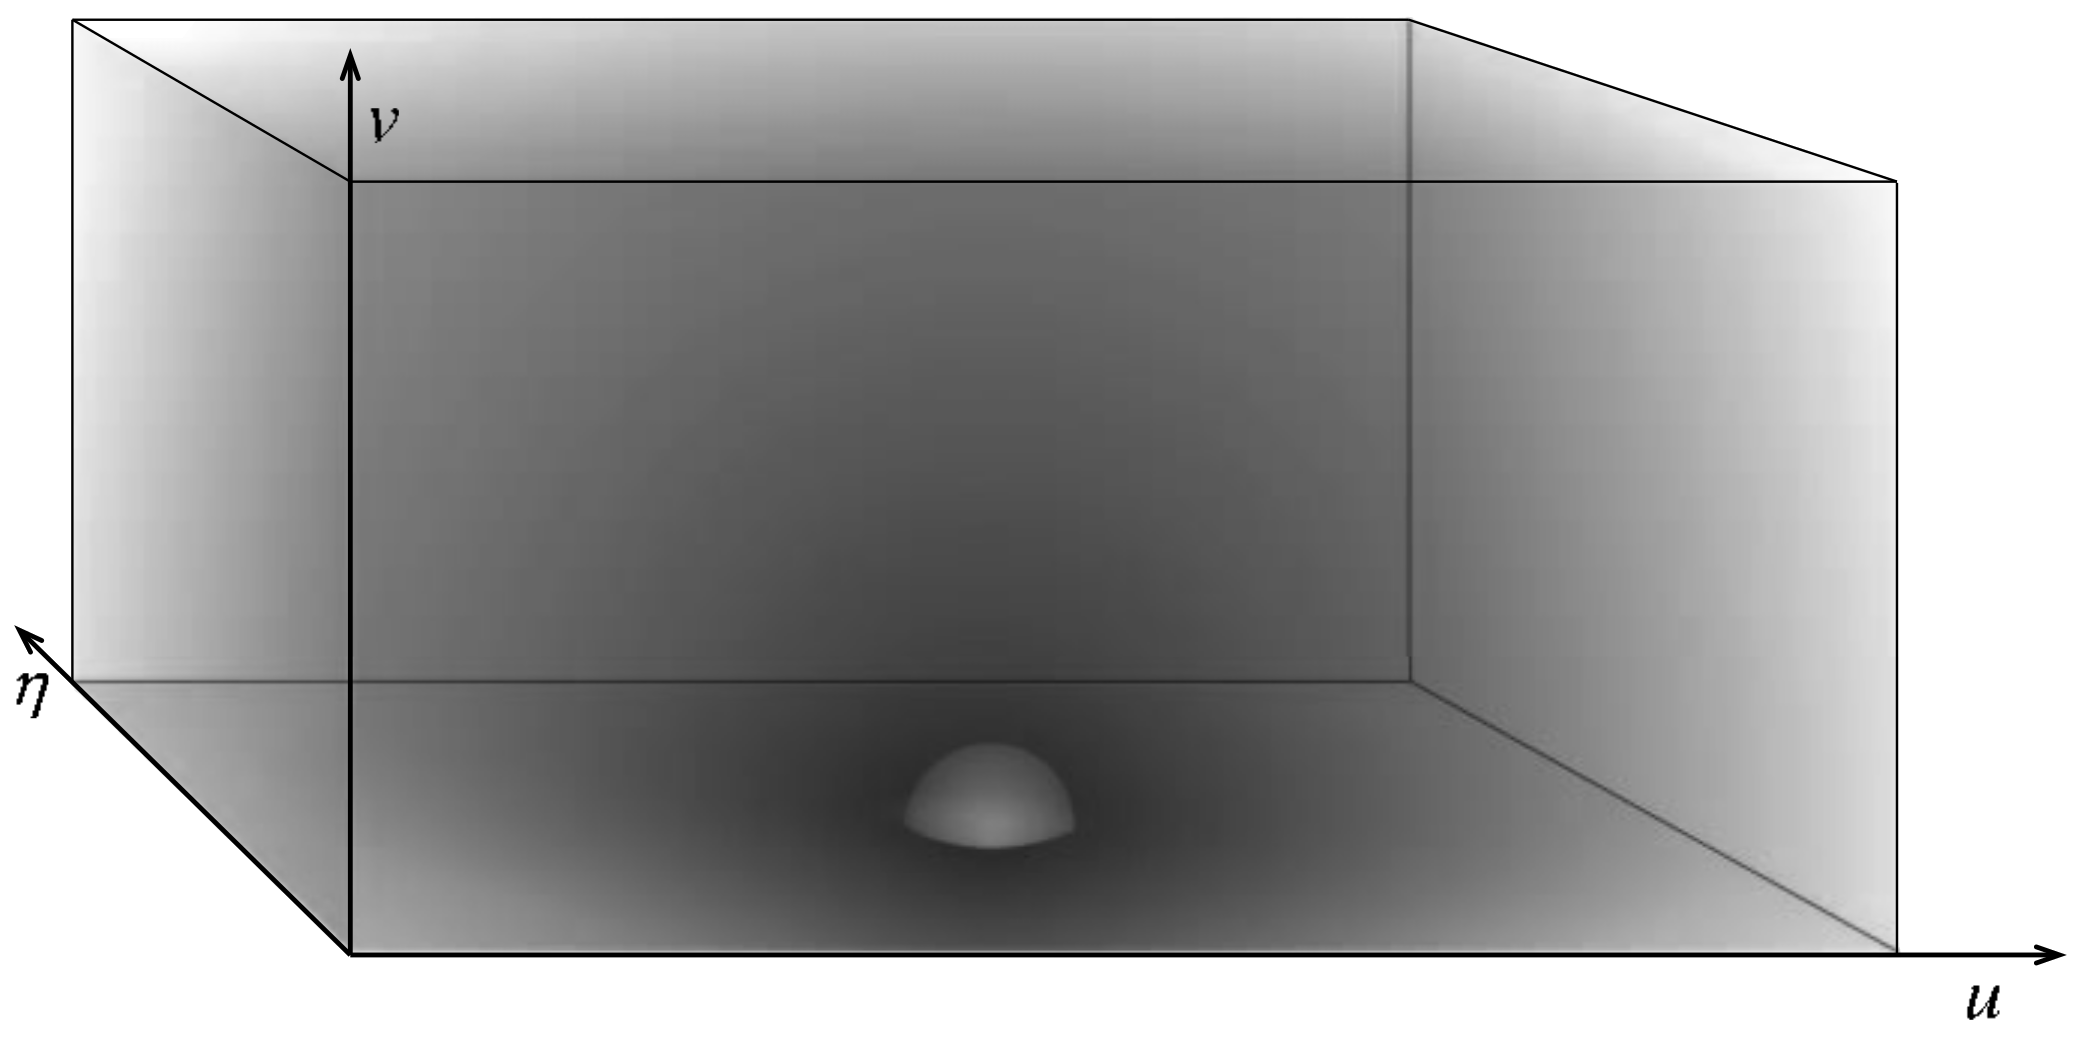
\includegraphics[width=0.5\textwidth]{EoR-fourier}%
  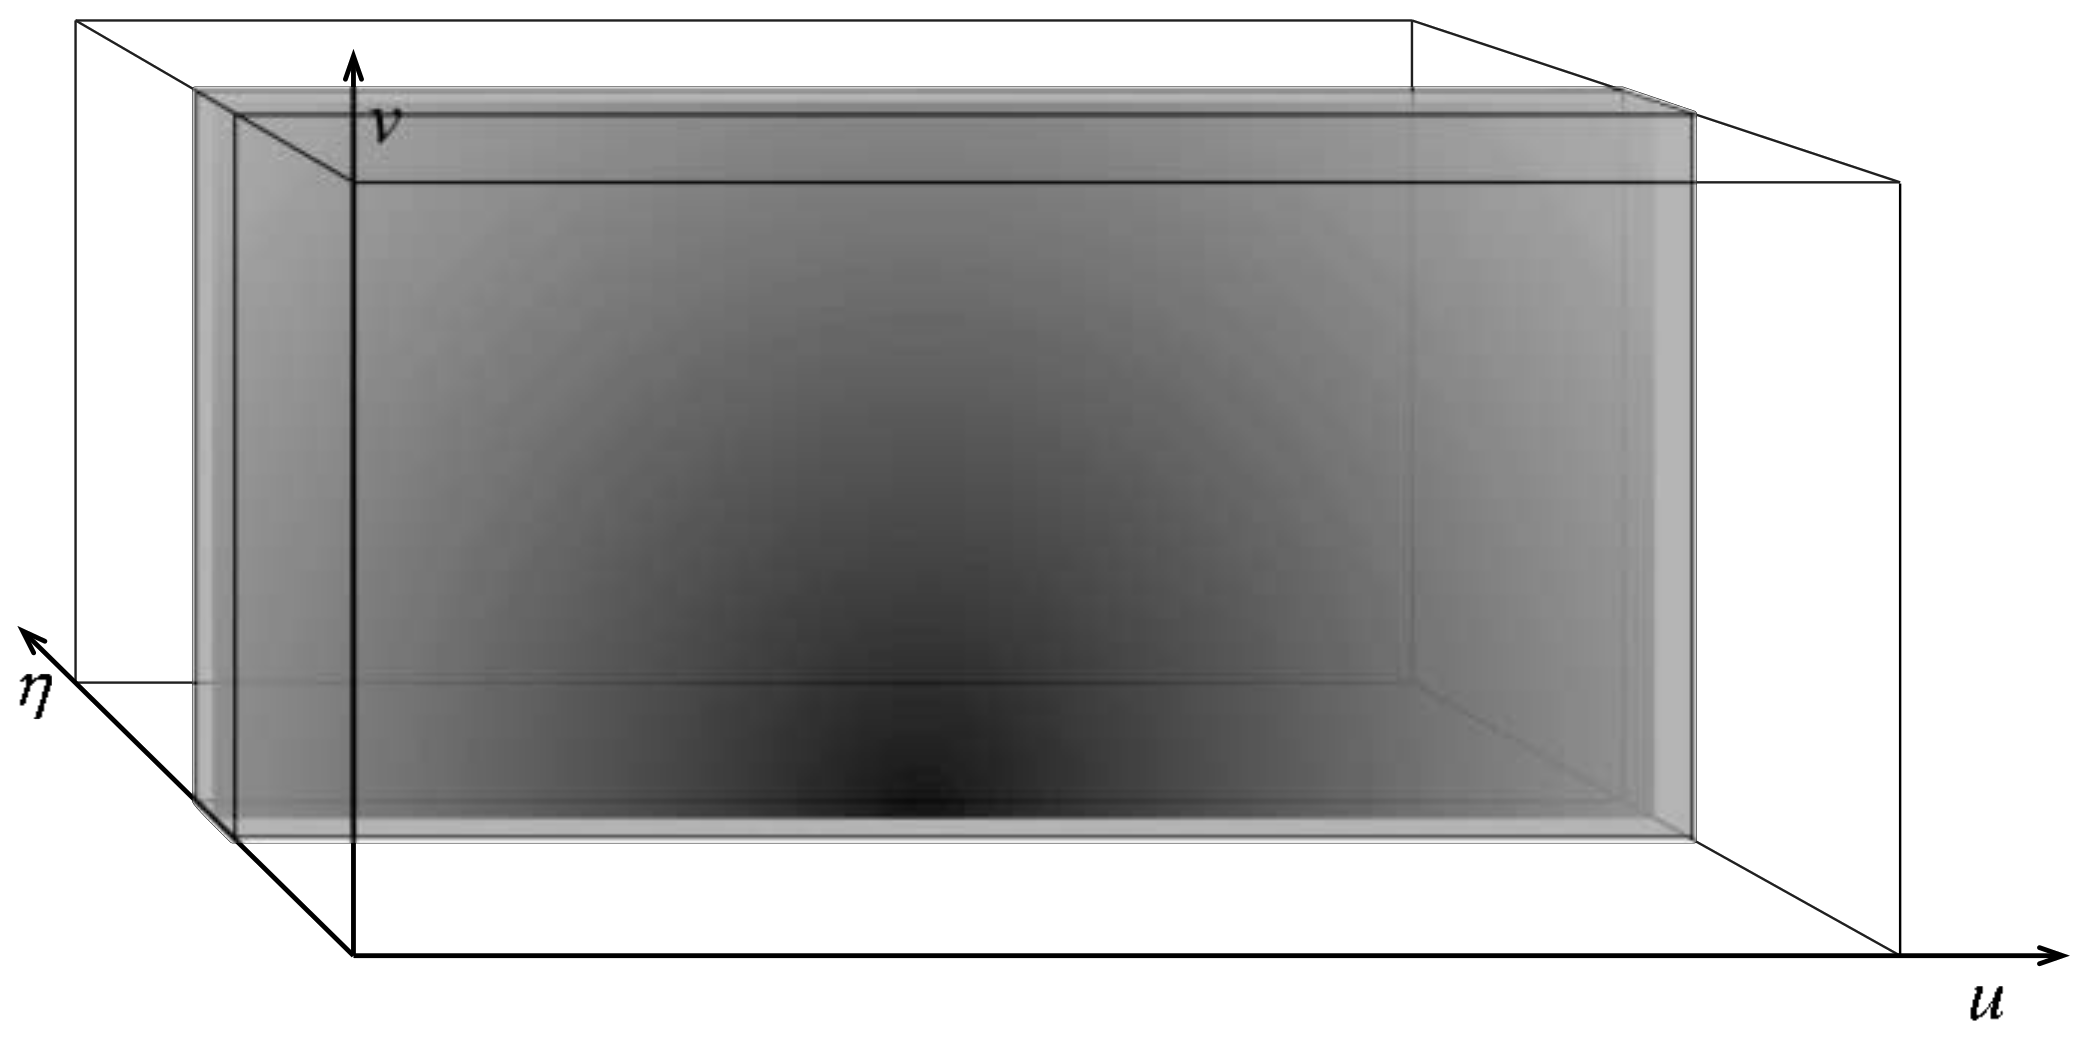
\includegraphics[width=0.5\textwidth]{foreground-fourier}
  \bicaption[EoR 信号和前景的三维功率谱示意图]{%
    \uline{(左栏)} EoR 信号的三维功率谱示意图,呈球对称分布.
    \uline{(右栏)} 前景辐射的三维功率谱示意图,
    可见功率在两个空间维度 ($u, v$) 的分布与在频率维度 ($\eta$) 的分布情况明显不同.
  }{%
    \emph{(Left)} An illustration of the \ac{3d} power spectrum
    of the EoR signal, exhibiting the spherical symmetry.
    \emph{(Right)} An illustration of the \ac{3d} power spectrum of the
    foreground emission, showing obviously different distributions in the
    spatial directions ($u, v$) and the frequency dimension ($\eta$).
    \\来源/Credit:
    \citeay{morales2004}.
  }
  \label{fig:eor-fg-fourier}
\end{figure}

当将红移范围限制在一个较窄的片段(如 $\Delta z \sim 0.5$)时,
可以忽略宇宙演化并认为中性氢的分布是各向同性的.
相应地,EoR 信号的三维功率谱 $\ac{psD}(\B{k})$ 则具有球对称分布
\cite{morales2004,mcQuinn2006},
如\autoref{fig:eor-fg-fourier} 左栏所示.
因此,可以将三维功率谱 $\ac{psD}(\B{k})$ 在一系列球壳里进行平均,
得到\emph{一维\ac{ps}} $\ac{psD}(k)$ \cite{morales2004,datta2010},
其中 $k = |\B{k}| = \sqrt{|\B{k}_{\perp}|^2 + k_{\parallel}^2}$ 为球壳的半径.
通过这种方式,EoR 信号的信息被有效地压缩到少量 Fourier \ac{mode}里,
极大地提高了每个\ac{mode}里 EoR 信号的\ac{snr},
从而大大降低了探测 EoR 信号的难度和所需的观测时间 \cite{datta2010}.

然而,实际观测中存在目前无法完全扣除的前景干扰.
尽管前景辐射的频谱是光滑的,但是具有非常复杂的空间结构
(如银河系的子结构、形态各异的射电星系、星系团弥散辐射;详见 \autoref{sec:fg-intro}),
因此,在三维功率谱中,前景辐射的功率将被较好地约束在频率维度
($\eta$ 或 $k_{\parallel}$),
但却弥散在整个空间维度 ($\B{u}$ 或 $\B{k}_{\perp}$),
如\autoref{fig:eor-fg-fourier} 右栏所示.
当简单地对三维功率谱按球壳平均时,
前景辐射将出现在所有的 $k$ \ac{mode}里,淹没 EoR 信号.

\begin{figure}[htp]
  \centering
  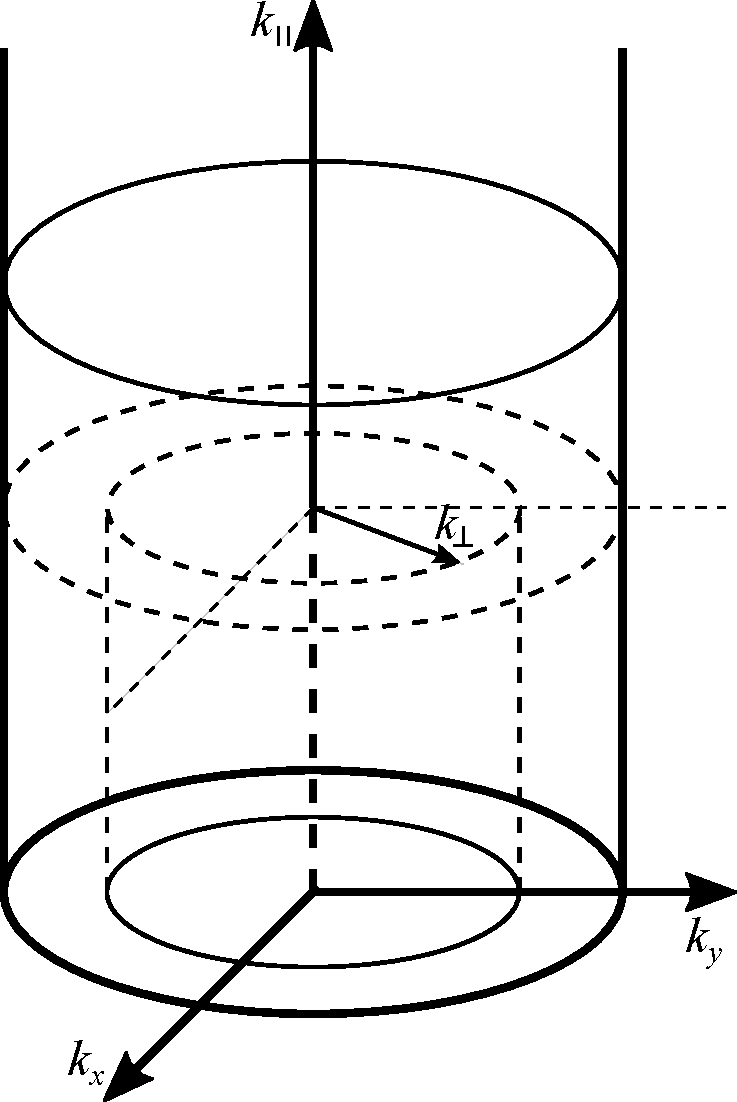
\includegraphics[width=0.35\textwidth]{ps2d-annuli-diagram}
  \bicaption[计算二维功率谱的示意图]{%
    计算二维功率谱 $\ac{psD}(k_{\perp}, k_{\parallel})$ 的示意图:
    在三维功率谱 $\ac{psD}(\B{k}_{\perp}, k_{\parallel})$
    的每一个 $k_{\parallel}$ 平面里,
    按一系列圆环(半径为 $k_{\perp} = |\B{k}_{\perp}|$)将功率平均.
  }{%
    A diagram showing the calculation of the \ac{2d} power spectrum
    $\ac{psD}(k_{\perp}, k_{\parallel})$:
    in each $k_{\parallel}$ plane of the \ac{3d} power spectrum,
    average the powers in a series of annuli with radius of
    $k_{\perp} = |\B{k}_{\perp}|$.
    \\来源/Credit:
    \citeay{thyagarajan2013}.
  }
  \label{fig:ps2d-calculation}
\end{figure}

EoR 信号的\ac{imgcube} $I_{\R{eor}}(\B{\theta}, \nu)$
的三个维度在本质上是相同的,均映射为中性氢的空间坐标.
但是对于前景的\ac{imgcube} $I_{\R{fg}}(\B{\theta}, \nu)$,
频率维度 $\nu$ 表示前景源的辐射频谱(通常为连续谱),
与两个空间维度 $\B{\theta}$ 完全不同,两者之间也是相互独立的.
因此,一个更好的处理方法是保持三维功率谱 $\ac{psD}(\B{k}_{\perp}, k_{\parallel})$
的频率维度 $k_{\parallel}$ 不变,只将两个空间维度 $\B{k}_{\perp}$ 压缩至一维.
具体而言:
如\autoref{fig:ps2d-calculation} 所示,
在三维功率谱的每一个 $k_{\parallel}$ 平面里,取一系列圆环将功率平均,
得到\emph{二维功率谱} $\ac{psD}(k_{\perp}, k_{\parallel})$,
其中 $k_{\perp} = |\B{k}_{\perp}|$ 是圆环的半径 \cite{datta2010,thyagarajan2013}.

在二维功率谱上,EoR 信号因具有不光滑的频谱而主要分布在 $k_{\parallel}$ 较大的区域,
频谱光滑的前景则主要分布在 $k_{\parallel}$ 较小的区域.
因此,可以在二维功率谱上避开那些受前景严重污染的区域,
在相对干净的区域开展 EoR 信号的探测和研究,
这为克服强烈的前景干扰提供了一条非常有效的途径.
由于这个独特优势,二维功率谱目前已成为分析 EoR 观测数据的最常用工具之一
\cite{trott2012,thyagarajan2013,barry2016,beardsley2016,trott2016,patil2017}.


%=====================================================================
\section{探测方法}
\label{sec:det-methods}

目前探测 EoR 信号的方法主要有以下三种,由易到难分别为:
\begin{enumerate}
  \item 测量全天总功率;
  \item 测量功率谱;
  \item 直接获取再电离区域的图像,即 EoR \ac{tomography}.
\end{enumerate}

第一种方法仅测量 EoR 信号的全天总功率随红移(即观测频率)的变化,
所得结果可以用于推断宇宙的电离过程,帮助检验和约束再电离模型
\cite{pritchard2012,liu2016}.
该方法相对简单易行,通常采用小型专用设备,一般只包含单个或少量天线.
目前已有一批采用该方法的 EoR 探测实验,主要包括
位于澳大利亚的 \ac{edges} \cite{bowman2008} 和
\ac{bighorns} \cite{sokolowski2015}、
位于美国的 \ac{leda} \cite{greenhill2012}、
位于墨西哥的 \ac{sci-hi} \cite{voytek2014}
以及位于印度的 \ac{saras} \cite{singh2018}.
值得一提的是,\acs{edges} 在 2018 年初报导称
发现全天平均的辐射信号在 \SI{78}{\MHz}附近存在吸收,
该吸收特征的位置大致符合早期恒星所引发的 21\,cm 信号,
但强度是目前理论预测值的两倍以上 \cite{bowman2018}.

后两种方法则进一步测量 EoR 信号的统计分布规律甚至三维图像,能够提供更加全面丰富
的信息用于系统性地研究\acl{eor}.
尽管这两种测量方法更加强大有效,但需要高灵敏度的大型低频干涉阵列,
而且目前仅有 SKA1-Low 将拥有足够高的灵敏度实现对再电离区域的直接成像观测.


%=====================================================================
\section{主要困难}
\label{sec:det-difficulties}

EoR 探测实验,尤其是采用干涉阵列,面临着一系列困难.
这些困难可主要分为以下几个方面:
\begin{itemize}
\item
\emph{前景干扰:}
源自银河系以及河外源的前景辐射非常强烈,亮温度可达数百 \si{\kelvin},
是 EoR 信号(亮温度仅约几 \si{\mK} 至几十 \si{\mK})的 \numrange{4}{5} 个数量级
\cite{morales2010}.
虽然干涉阵列只能测量辐射的空间涨落幅度而非其绝对强度 \cite{braun1985},
但是前景辐射的涨落幅度仍达数 \si{\kelvin} 到数十 \si{\kelvin},
远远压制了待测 EoR 信号 \cite{zaroubi2013}.
\autoref{fig:eor-foregrounds} 显示了主要的前景成分及其在 \SI{120}{\MHz} 处的强度.
因此,即便是轻微的前景处理不当,都会导致微弱的 EoR 信号被淹没而无法被提取出来.
此外,部分前景成分(如银河系\ac{rad-syn})存在一定程度的偏振,
该偏振成分可能发生泄漏而影响前景的总强度的测量,
即\ac{pl}效应 \cite{cotton1999,reid2008},
导致前景的频谱结构复杂化而变得更加难以处理
\cite{jelic2014,asad2015,asad2016,asad2018,gehlot2018}.
如何处理强烈的前景干扰并成功提取 EoR 信号,
是目前 EoR 探测领域的一个关键任务,
不仅需要系统深入地理解各个前景成分的特征
\cite{jelic2008,jelic2010,wang2010,liu2012,offringa2016,
  carroll2016,murray2017,procopio2017,spinelli2018},
还需要研发有效的前景扣除与信号分离算法
\cite{wang2006,jelic2008,harker2009,liu2009fgrm,chapman2012,chapman2013,
  gu2013,wang2013,bonaldi2015,chapman2015,chapman2016,mertens2018}.

\begin{figure}[htp]
  \centering
  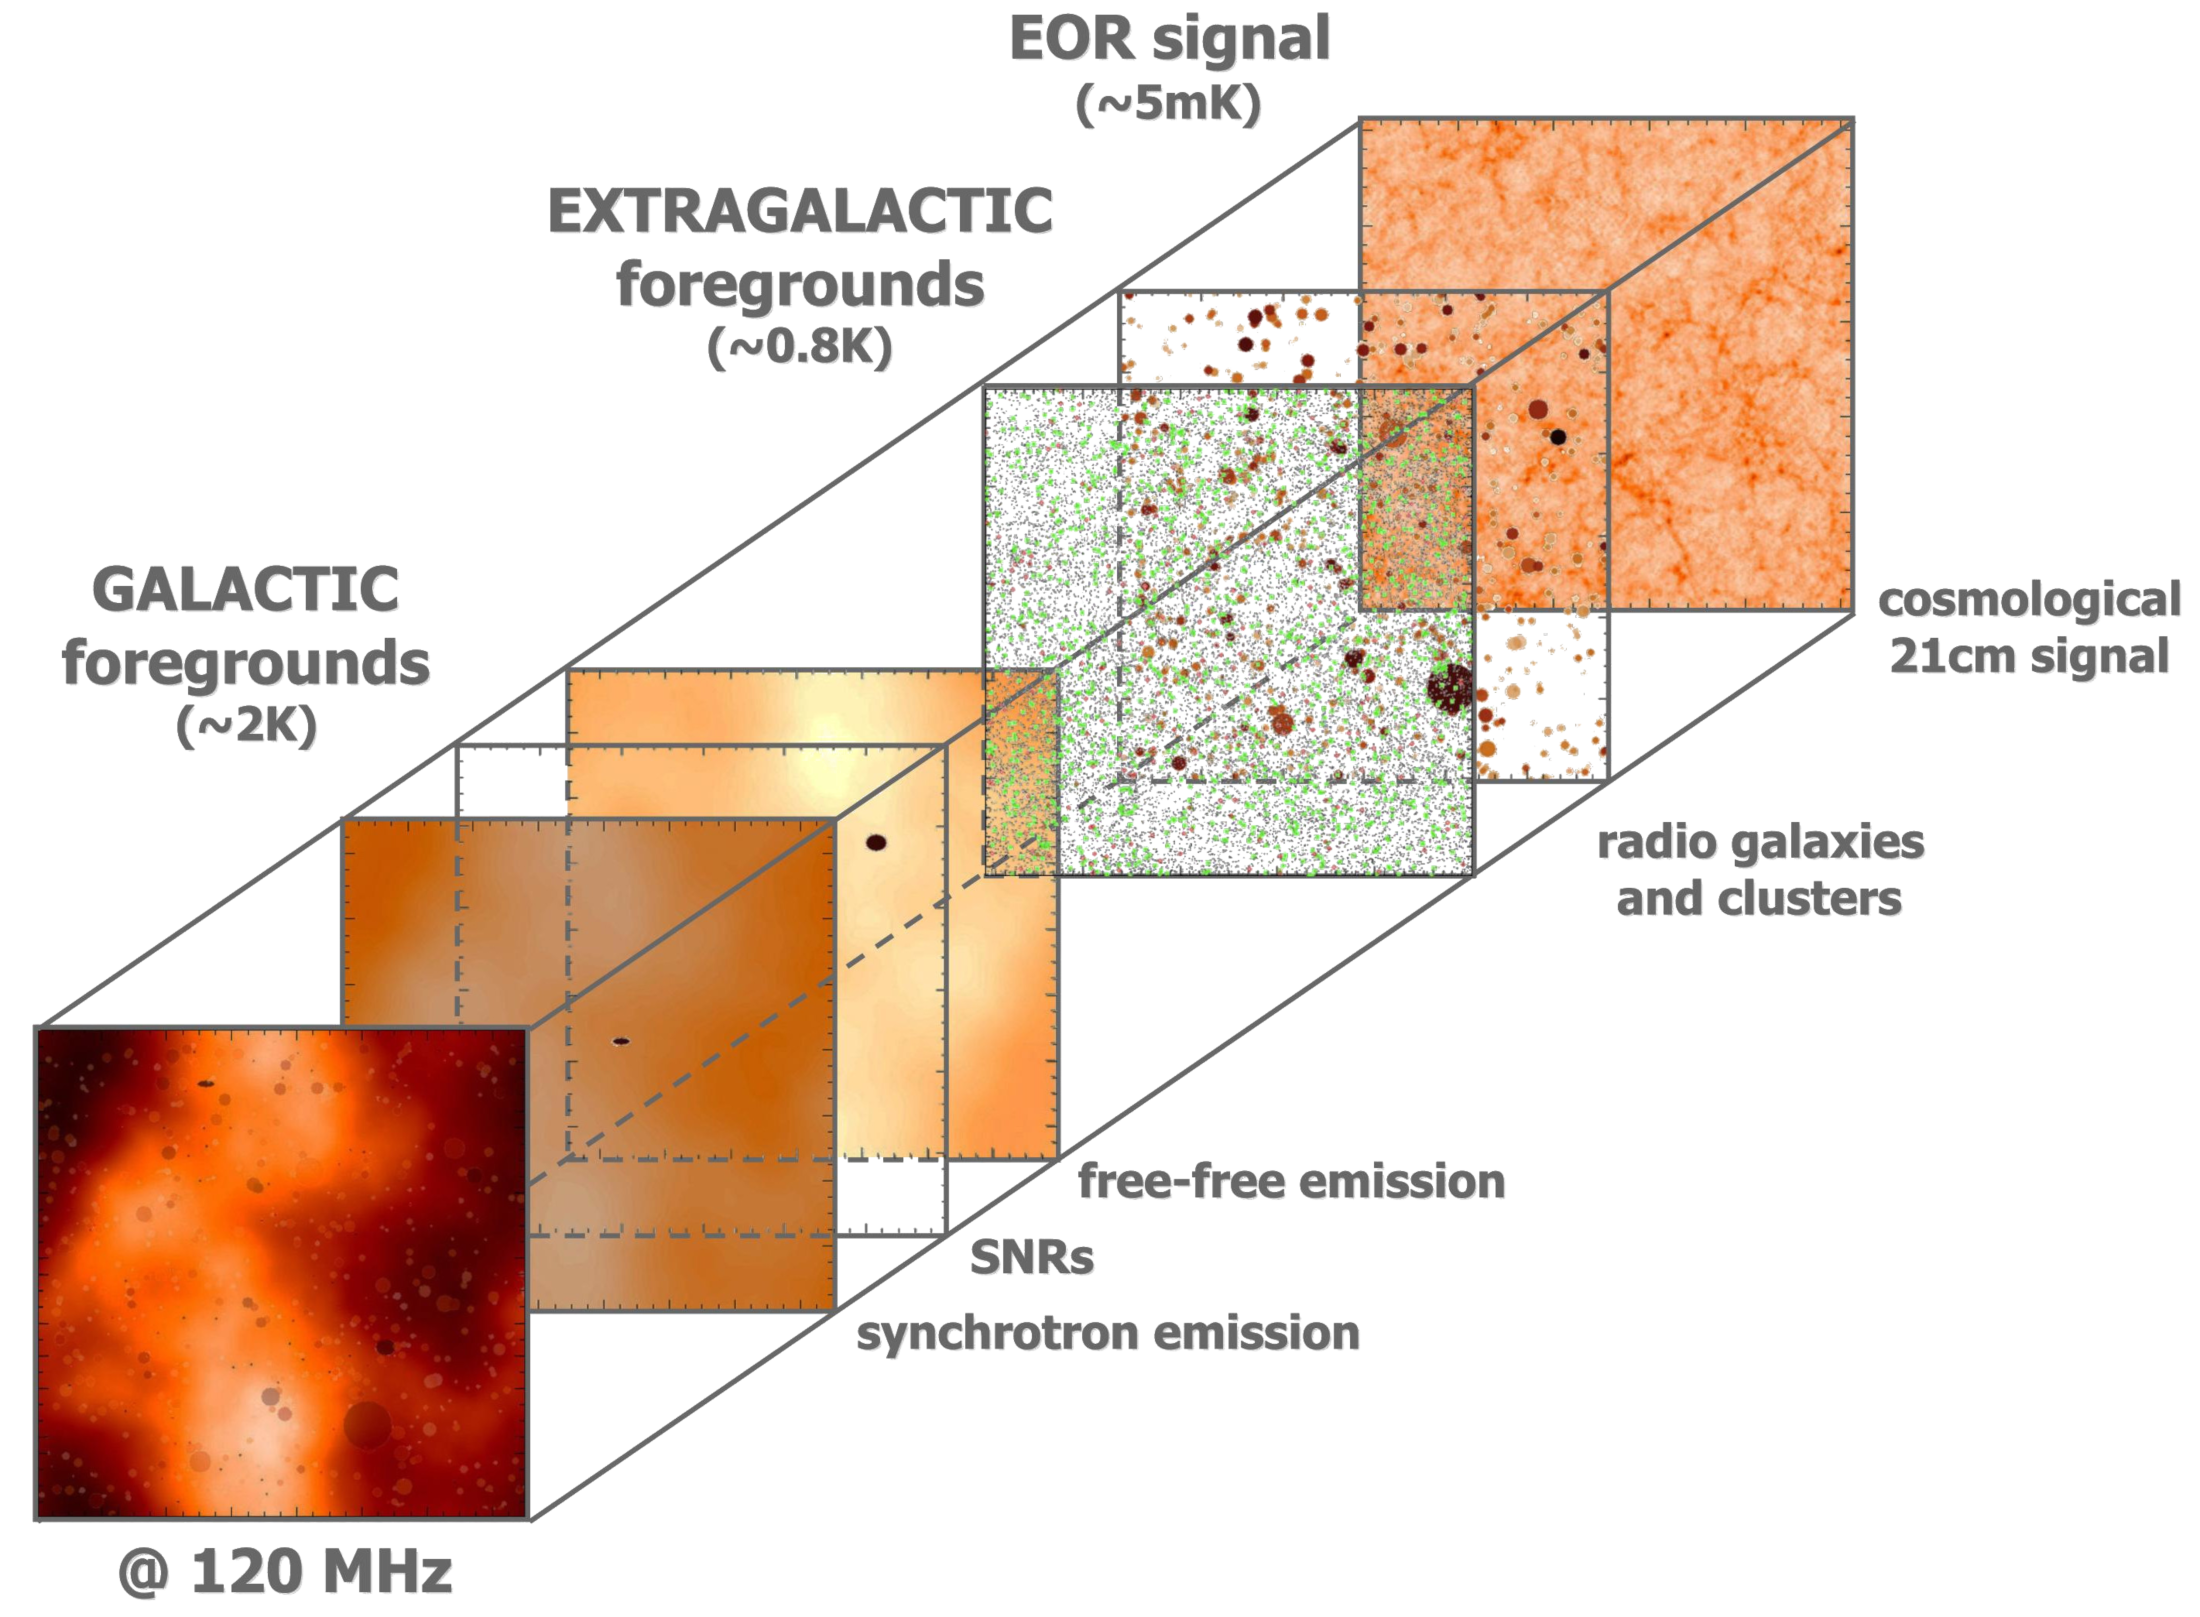
\includegraphics[width=0.7\textwidth]{eor-foregrounds}
  \bicaption[主要前景成分及其强度示意图]{%
    主要前景成分以及强度示意图.
    图中的数值代表在 \SI{120}{\MHz} 处的\acs*{rms}值.
  }{%
    A diagram showing the major foreground components contaminating
    the EoR signal.
    The numbers in the figure represent the root-mean-square values
    at \SI{120}{\MHz}.
    \\来源/Credit:
    \citeay{zaroubi2013}, \S\,5.5.
  }
  \label{fig:eor-foregrounds}
\end{figure}

%.......................................
\item
\emph{人工源的\acl{rfi}:}
人类活动产生的无线电波已在地球上无处不在,
对射电天文观测产生了严重的\acf{rfi}.
这些人工源主要有:\ac{am}和\ac{fm}广播、卫星通信、\ac{gps} 信号、
对讲机、手机、移动通信基站、航空通信、雷达、等等.
虽然 EoR 探测设备通常建设在人烟稀少的射电宁静区域,
但是仍不可避免也受到人工源的 \ac{rfi},
甚至由月亮以及太空碎片反射回来的无线电波都可能对 EoR 观测产生一定程度的影响
\cite{mcKinley2013,tingay2013rfi}.
如\autoref{fig:rfi-mwa} 所示的是 MWA 在其各子频段的\ac{vis}数据
被标记为 \ac{rfi} 的比例,
其中突显了\ac{fm}广播、卫星通信以及数字电视等干扰源对 EoR 探测所造成的影响.
\ac{rfi} 的强度通常会高出天空信号的若干个数量级,并且会实时发生变化 \cite{bentum2011}.
目前常用的一种办法是识别并屏蔽存在明显 \ac{rfi} 的时间和频率片段
\cite{fridman2001,offringa2010,offringa2012,prasad2012,akeret2017},
但是残留的干扰可能会对前景处理以及 EoR 信号的测量均产生严重影响 \cite{offringa2015}.

\begin{figure}[htp]
  \centering
  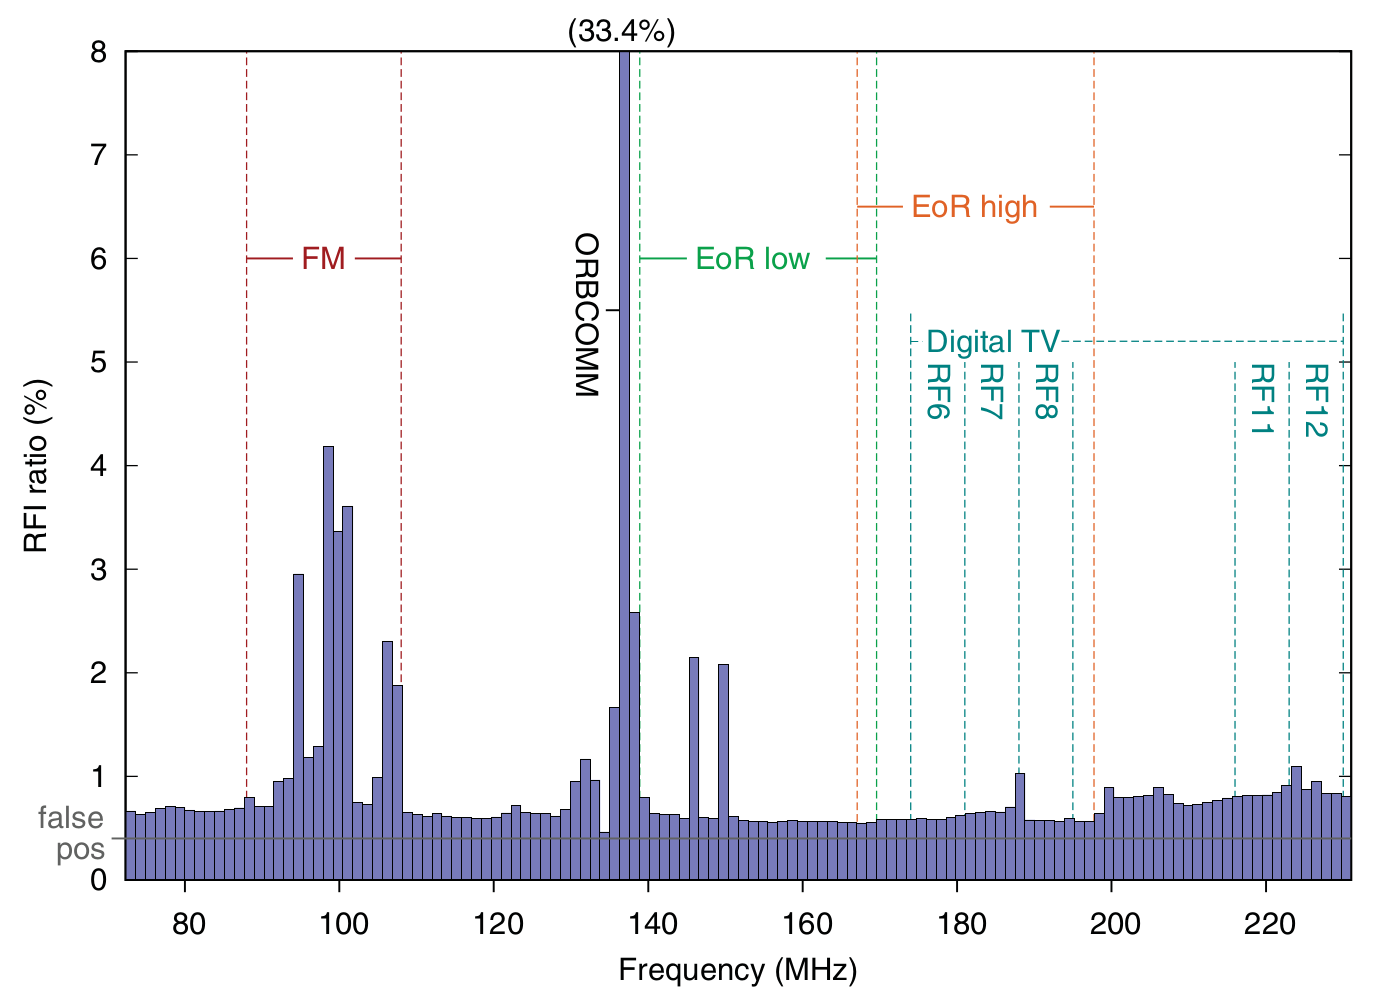
\includegraphics[width=0.7\textwidth]{RFI-MWA}
  \bicaption[MWA 各子频段内的 RFI 比例]{%
    MWA 各子频段的\acs*{vis}数据被标记为 \acs*{rfi} 的比例.
  }{%
    The \acs*{rfi} occupancy, calculated as the percentage of
    visibilities that are detected as \acs*{rfi} by the flagger,
    per sub-band for the MWA.
    \\来源/Credit:
    \citeay{offringa2015}.
  }
  \label{fig:rfi-mwa}
\end{figure}

%.......................................
\item
\emph{电离层干扰:}
\acf{ionosphere}是地球大气层顶部被太阳辐射电离的部分,
从约 \SI{60}{\km} 延伸至约 \SI{1000}{\km} 的高空,
覆盖了大气层的部分\ac{mesosphere}、\ac{thermosphere}以及\ac{exosphere},
如\autoref{fig:ionosphere} 所示.
电离层的气体非常稀薄,因此被太阳辐射电离的气体分子所产生的自由电子
在复合前可以短暂地自由运动,形成等离子体,从而影响电磁波的传播.
在 $<$\,\SI{300}{\MHz} 的低频波段,电离层主要对电磁波产生折射、
传播延迟、Faraday 旋转等影响,导致望远镜的观测数据出现相位和幅度误差
\cite{intema2009,thompson2017}.
由于主要受太阳活动的影响,电离层的状态会随时间和位置而发生剧烈变化,
因此对干涉阵列各个天线产生的干扰程度也存在差异并且时刻发生变化.
为了获得高质量的图像,必须实时校准观测数据 \cite{intema2009,jordan2017}.
这将成为 \ac{lofar}、\ac{mwa}、\ac{ska} 等大型低频干涉阵列的一个严重的计算负担
\cite{intema2009,deGasperin2018}.

\begin{figure}[htp]
  \centering
  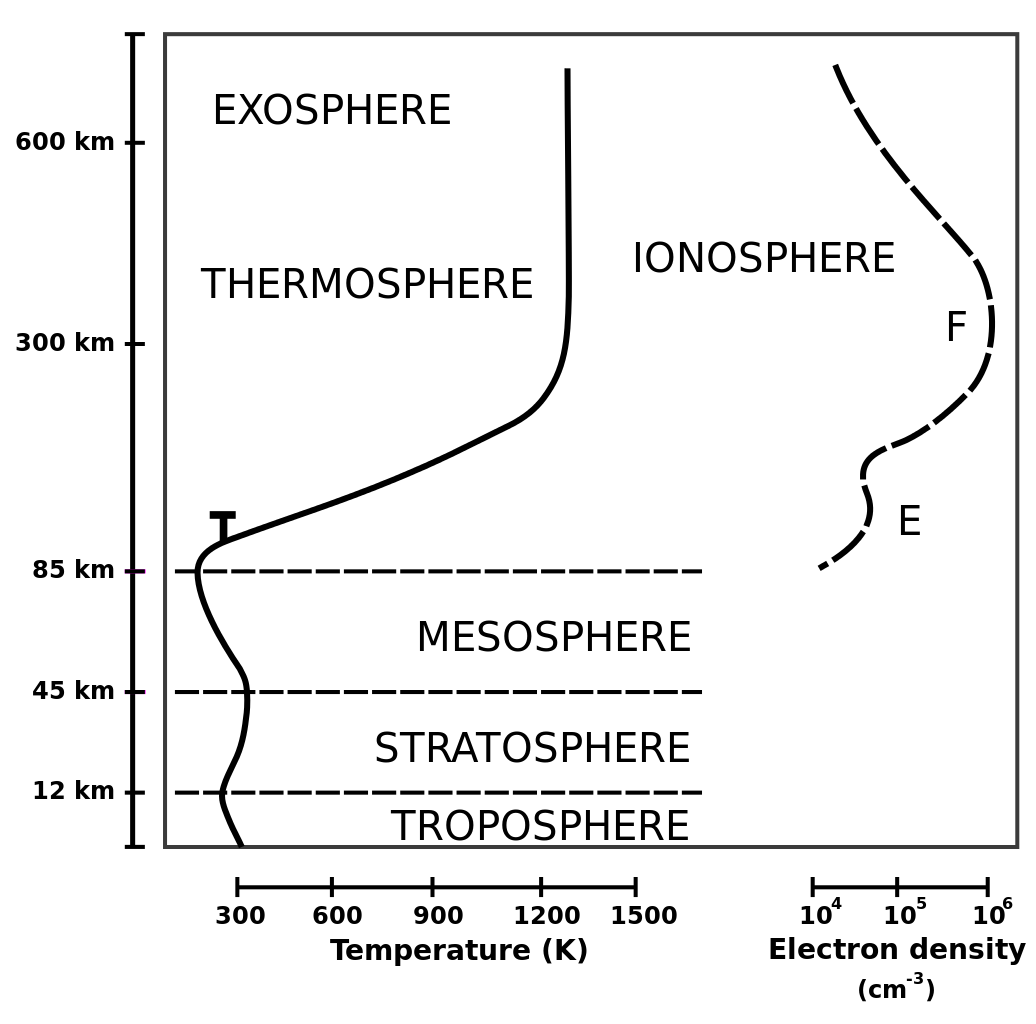
\includegraphics[width=0.5\textwidth]{atmosphere-with-ionosphere}
  \bicaption[大气层和电离层的关系]{%
    地球的大气层和电离层之间的关系.
    电离层是大气层顶部被太阳辐射电离的部分.
  }{%
    The relation between Earth's atmosphere and ionosphere, which
    is the ionized part of upper atmosphere.
    \\来源/Credit:
    Bhamer,
    \url{https://en.wikipedia.org/wiki/File:Atmosphere_with_Ionosphere.svg},
    (2018-10-13), 公有领域.
  }
  \label{fig:ionosphere}
\end{figure}

%.......................................
\item
\emph{仪器效应:}
当代的干涉阵列通常由成千上万根天线组成. 由于生产和安装过程的差异以及随环境和时间的变化,
\ac{station}内每根天线的性能都不可能完全相同,
导致所形成的\ac{beam-station}存在很多不确定因素,
而且各个\ac{station}的波束也互不相同.
对于采用数字\ac{beam-forming}技术的\ac{phased-array}而言,
波束的形态更会随着所指方向而发生大幅变化
\cite{smirnov2011iii,vanWeeren2016,jagannathan2017}.
因此,如果未能充分地地校准\ac{beam-station},那么后续其他仪器效应的校准、
亮点源的剥离 (peeling)、前景去除等任务都会受到严重影响 \cite{noordam2004,neben2016}.
除了\ac{beam-station}的效应,还有一系列更复杂的仪器效应,比如:
显著的旁瓣 \cite{thyagarajan2015,mort2017}、
天线响应随频率的变化 \cite{bernardi2015,trott2017}、
波束的频率依赖效应 \cite{liu2009ps,datta2010,morales2012}
(另见 \autoref{sec:eor-window} 和 \autoref{sec:beam-effect})、
\ac{pl} \cite{asad2015,asad2016,asad2018,lenc2017}、
信号在电缆内的反射 \cite{beardsley2016}.
如何准确有效地校准仪器,发挥出仪器的设计性能,是目前最迫切的任务之一
\cite{noordam2004,mitchell2008,wijnholds2010,barry2016,dillon2016}.

%.......................................
\item
\emph{海量数据:}
大型干涉阵列将产生海量数据,如 SKA1-Low 的数据流量预计高达 $\sim$\,1\,TB/s,
由此引发一系列难题 \cite{norris2011,dolensky2016,chrysostomou2018},
比如:
如何对原始数据进行实时的相关和校准?
如何传输、分发和存储海量观测数据?
如何实现高效的数字\ac{beam-forming}和多波束技术?
如何处理海量数据实现大视场高动态范围成像?
缓解或解决这些问题,不仅依赖于更快更高效的计算资源 \cite{magro2014,vermij2017},
建设新型的数据中心 \cite{chrysostomou2018},
还需要研发新算法以及编写新软件,优化数据处理流程,充分利用大规模并行计算资源
\cite{morales2009,bonaldi2018,farnes2018,gunst2018}.

\end{itemize}


%=====================================================================
\section{主要前景成分}
\label{sec:fg-intro}

%---------------------------------------------------------------------
\subsection{银河系同步辐射}

\emph{银河系\acs{rad-syn} (Galactic synchrotron radiation)}
是由弥散于银河系内的高能带电粒子在磁场中发生加速运动而产生的,
是低频射电波段 ($\gtrsim$\,\SI{1}{\GHz}) 最明亮的前景成分
\cite{bernardi2009,ghosh2012}.
在 \SI{150}{\MHz} 处,即使是高银纬辐射较弱的区域,
银河系同步辐射亦占全部前景辐射的 $\sim$\,70\% \cite{shaver1999}.
\autoref{fig:galactic-syn} 上栏显示了由 \citeay{remazeilles2015}
重新处理的 Haslam \SI{408}{\MHz} 巡天图 \cite{haslam1982},
可见银河系同步辐射具有明显的大尺度(约在度以上)子结构,
这将在\ac{ps}的大尺度区域对 EoR 信号产生严重污染.

银河系同步辐射的频谱近似为幂律形式,但谱指数随天空区域而变化,
如\autoref{fig:galactic-syn} 下栏所示.
在高银纬区域,\SIrange{100}{200}{\MHz} 范围内的平均谱指数
$\acs{spec-index}_{\R{syn}} \sim \num{2.5 +- 0.1}$ \cite{rogers2008}.

\begin{figure}[htp]
  \centering
  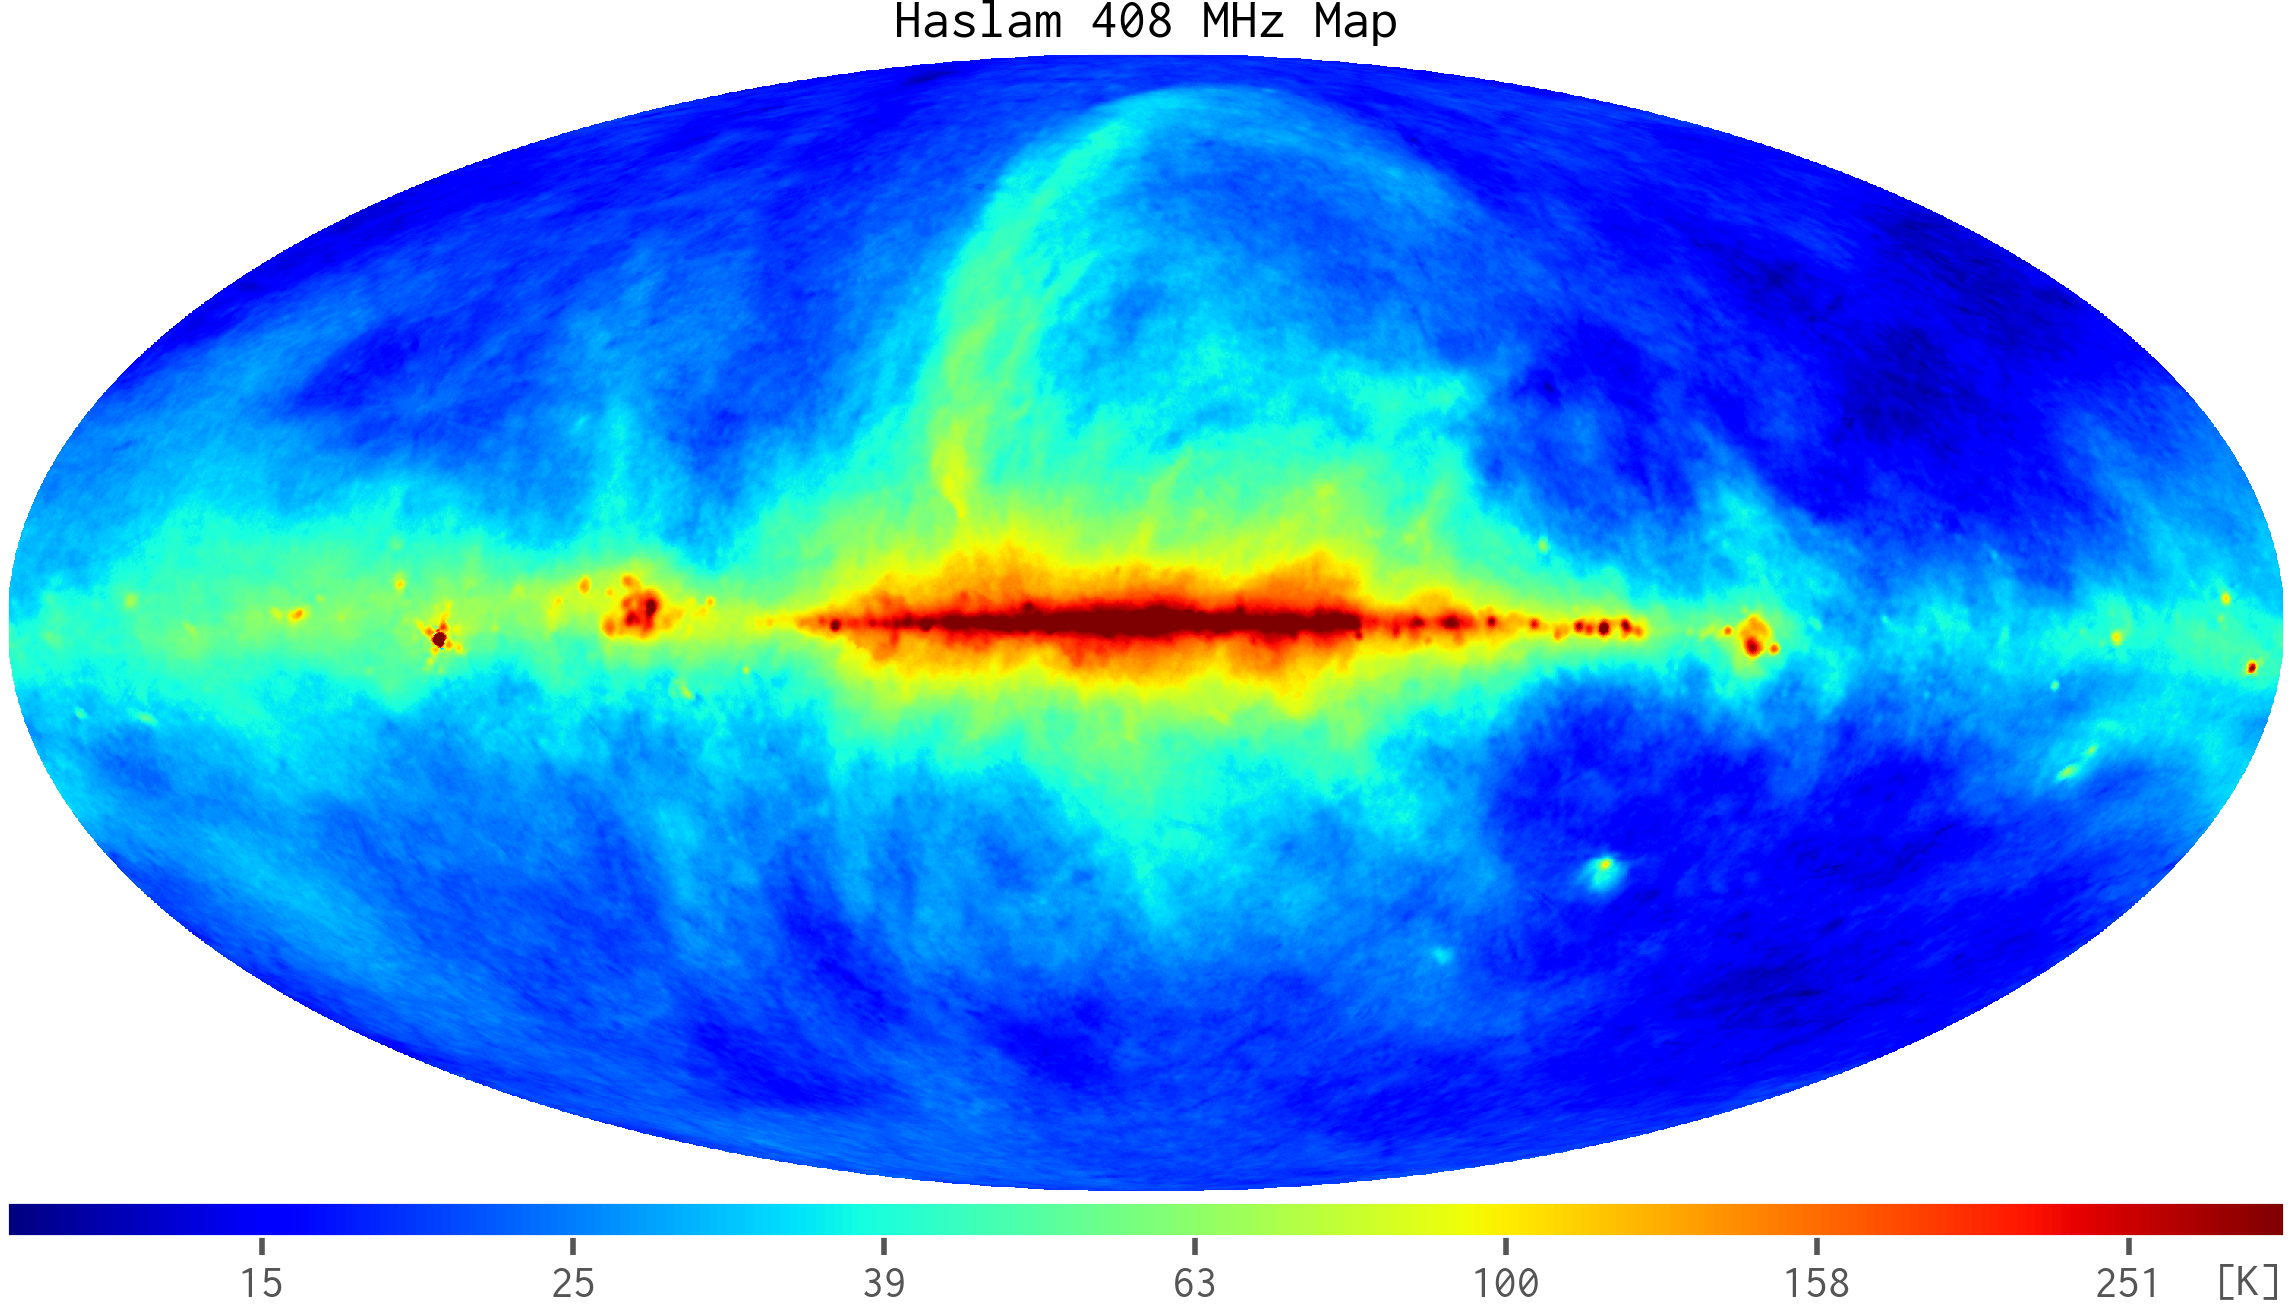
\includegraphics[width=0.95\textwidth]{galactic-haslam408}
  \\\medskip
  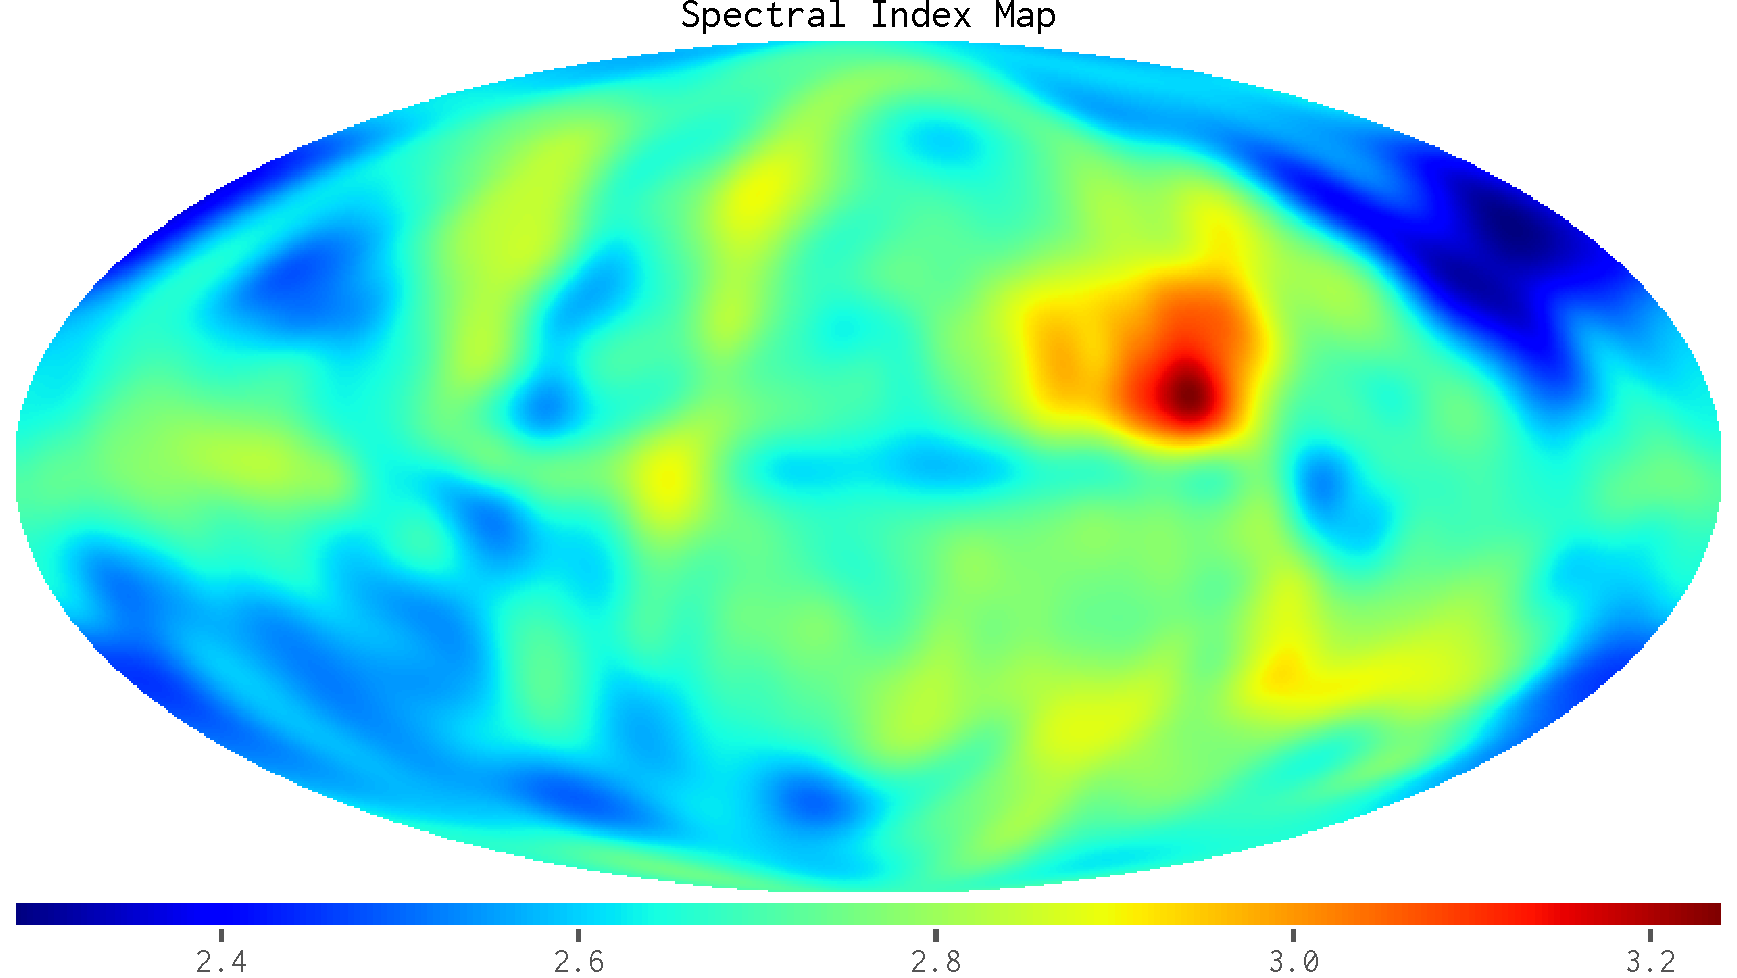
\includegraphics[width=0.95\textwidth]{galactic-spec-index}
  \bicaption[银河系同步辐射的 \SI{408}{\MHz} 巡天图和谱指数图]{%
    \uline{(上栏)}
    由 \citeay{remazeilles2015} 重新处理的 Haslam \SI{408}{\MHz} 巡天图,
    显示了银河系同步辐射的强度分布.
    \uline{(下栏)}
    由 \citeay{giardino2002} 处理得到的银河系同步辐射的谱指数全天分布图,
    利用了 \SI{408}{\MHz} 全天图、\SI{1420}{\MHz} 北天图 \cite{reich1986}
    以及 \SI{2326}{\MHz} 南天图 \cite{jonas1998}.
  }{%
    \emph{(Upper)} The Haslam \SI{408}{\MHz} all-sky map
    reprocessed by \citeay{remazeilles2015} shows the
    Galactic synchrotron radiation.
    \emph{(Lower)} The synchrotron spectral index map obtained
    by \citeay{giardino2002} by utilizing the \SI{408}{\MHz} all-sky map,
    the \SI{1420}{\MHz} northern sky survey \cite{reich1986}, and
    the \SI{2326}{\MHz} southern sky survey \cite{jonas1998}.
  }
  \label{fig:galactic-syn}
\end{figure}

在低频射电波段对银河系同步辐射的观测和研究仍然非常有限,
目前仅对少数几个天区开展了深入观测和研究
\cite{bernardi2009,ghosh2012,iacobelli2013,choudhuri2017},
基于大规模巡天的研究更是匮乏.
由于磁场强度的涨落、高能带电粒子的密度涨落、\ac{ism}的湍流等因素的影响
\cite{waelkens2009,lazarian2012syn,iacobelli2013},
银河系同步辐射应具有更复杂的小尺度(角分及亚角分)结构.
但是受限于目前的观测数据(Haslam \SI{408}{\MHz} 全天图的分辨率约为 \SI{0.85}{\degree}),
我们对这些细节的了解程度远远不够 \cite{ali2016}.

另一方面,银河系同步辐射具有一定的偏振 \cite{bernardi2009,jelic2014,gehlot2018}.
偏振的辐射通过磁场时,其偏振面会发生旋转,即 Faraday 旋转效应 \cite{rybicki1979},
而且旋转量依赖于辐射频率.
因此天线接收到的某一偏振成分(如 Stokes $Q$ 或 $U$ 分量)的强度变化也依赖于频率,
使得其频谱可能变得不光滑.
同时,仪器因其固有的限制而无法完全隔离各偏振成分的测量,
因此会有少量 ($\sim$\,1\%) 偏振辐射\enquote{漏泄}到总辐射强度里,
从而对前景频谱的光滑性产生破坏,阻碍前景的准确扣除
\cite{jelic2010,alonso2014,nunhokee2017,gehlot2018,spinelli2018}.

%---------------------------------------------------------------------
\subsection{银河系自由--自由辐射}

\emph{银河系\acs{rad-ff} (Galactic free--free radiation)}
源自于银河系的\ac{hii}区、\ac{wim}等区域的热电子的\ac{rad-brem}.
因为电子在辐射前后都是自由的(即没有被束缚在离子、原子、分子里),
所以\ac{rad-brem}又被称为\emph{\ac{rad-ff}}.
银河系\ac{rad-ff}的谱指数 $\acs{spec-index}_{\R{ff}} \sim 2.1$,
比\ac{rad-syn}的频谱偏平一点 \cite{dickinson2003}.

在低频射电波段,除了银盘附近区域,
银河系\ac{rad-ff}被淹没在\ac{rad-syn}之中而无法被直接观测到,
所以我们对该辐射成分的了解非常有限.
目前已掌握的有关银河系\ac{rad-ff}的信息主要源自 Hα 巡天 \cite{finkbeiner2003},
因为产生\ac{rad-ff}的电离区域同时也会产生 Hα 辐射,
而且两种辐射的强度之间存在紧密关联,
因此可以利用 Hα 辐射来有效地追踪\ac{rad-ff} \cite{smoot1998,dickinson2003}.
不过 Hα 辐射容易被尘埃吸收,因此需要首先利用尘埃分布图\cite{schlegel1998}
对 Hα 辐射进行修正,然后再推导\ac{rad-ff} \cite{dickinson2003},
如\autoref{fig:galactic-ff} 显示了利用该方法(详见 \autoref{sec:simu-gff})
得到的银河系\ac{rad-ff}在 \SI{150}{\MHz} 的全天图.
但是在银盘附近,Hα 辐射的尘埃吸收修正将因为尘埃多、分布复杂而变得不可靠,
从而无法给出合理的\ac{rad-ff} \cite{dickinson2003}.

\begin{figure}[htp]
  \centering
  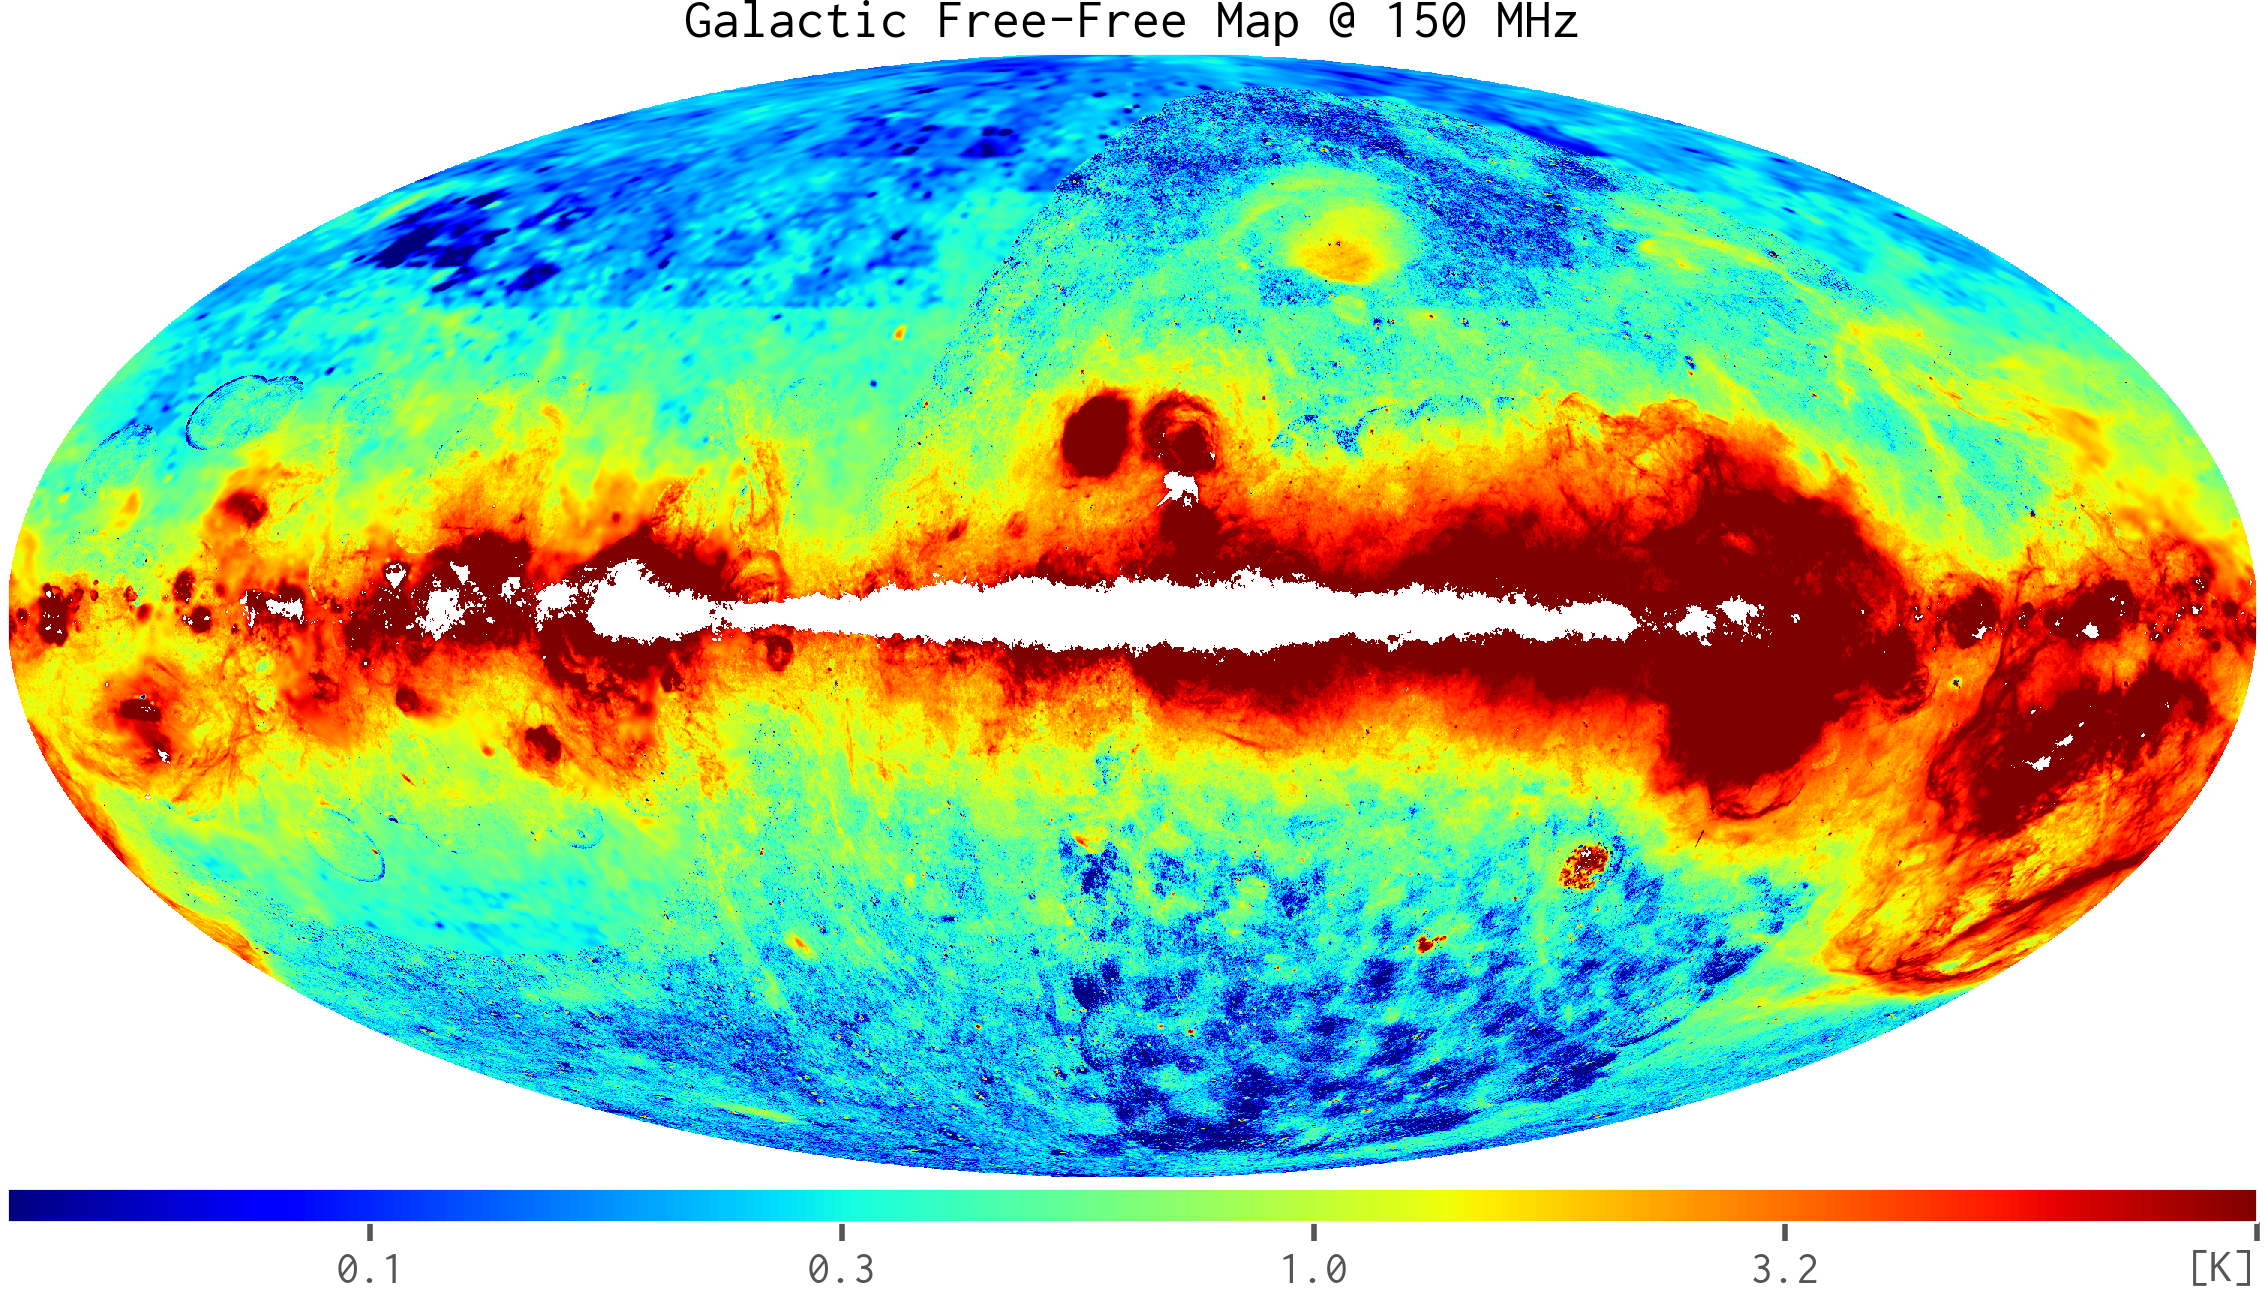
\includegraphics[width=0.95\textwidth]{galactic-freefree}
  \bicaption[银河系自由--自由辐射在 \SI{150}{\MHz} 的全天图]{%
    对 Hα 全天辐射图\cite{finkbeiner2003}修正尘埃吸收后得到的
    银河系自由--自由辐射在 \SI{150}{\MHz} 的强度分布图 \cite{dickinson2003}.
    图中靠近银盘的白色区域由于尘埃吸收修正不可靠而被屏蔽.
  }{%
    The Galactic free--free radiation map at \SI{150}{\MHz}
    derived from the Hα all-sky map \cite{finkbeiner2003}
    with dust absorption corrected \cite{dickinson2003}.
    The white regions near the Galactic plane are masked due to
    the large uncertainty about the correction for dust absorption.
  }
  \label{fig:galactic-ff}
\end{figure}

另一种追踪\ac{rad-ff}的方法是利用\ac{rrl}.
因为\ac{rrl}不受尘埃吸收的影响,所以该方法可以顺利也用于银盘附近区域,
给出可靠的\ac{rad-ff} \cite{alves2010,alves2012}.
与前面的方法相结合,可以获得银河系\ac{rad-ff}的完整全天图.

尽管银河系\ac{rad-ff}的强度远弱于同步辐射成分,
比如在 \SI{150}{\MHz} 处仅贡献了总前景辐射的 $\sim$\,1\% \cite{shaver1999},
但仍然是重要的 EoR 前景干扰成分,原因有二 \cite{jelic2008}:
(1) 该前景成分的强度和涨落仍然远强于 EoR 信号;
(2) 该前景成分的谱指数和子结构与其他前景成分不同.

%---------------------------------------------------------------------
\subsection{河外点源}

除银河系的弥散辐射(\ac{rad-syn}和\ac{rad-ff})之外,最强的前景干扰源
便是数目极多的\emph{河外\acs{src-point} (extragalactic point source)},
这些\ac{src-point}产生的辐射在 \SI{150}{\MHz} 处贡献了总前景辐射的
$\sim$\,27\% \cite{shaver1999}.
在\ac{ps}的小尺度(亚角分)区域,河外点源更是成为最强、最难处理的前景成分
\cite{murray2017,procopio2017,yoshiura2018}.
如\autoref{fig:mwa-eor0} 显示了 MWA 对 EoR0 天区\footnote{%
  MWA 针对 EoR 深度观测筛选了 3 块天区,
  中心坐标 (R.A., Dec.\@) 分别为 \cite{beardsley2016}:
  EoR0: (\SI{0}{\degree}, \SI{-27}{\degree});
  EoR1: (\SI{60}{\degree}, \SI{-27}{\degree});
  EoR2: (\SI{170}{\degree}, \SI{-10}{\degree}).
}的深度曝光图像 \cite{offringa2016},可见密布的点源.

\begin{figure}[htp]
  \centering
  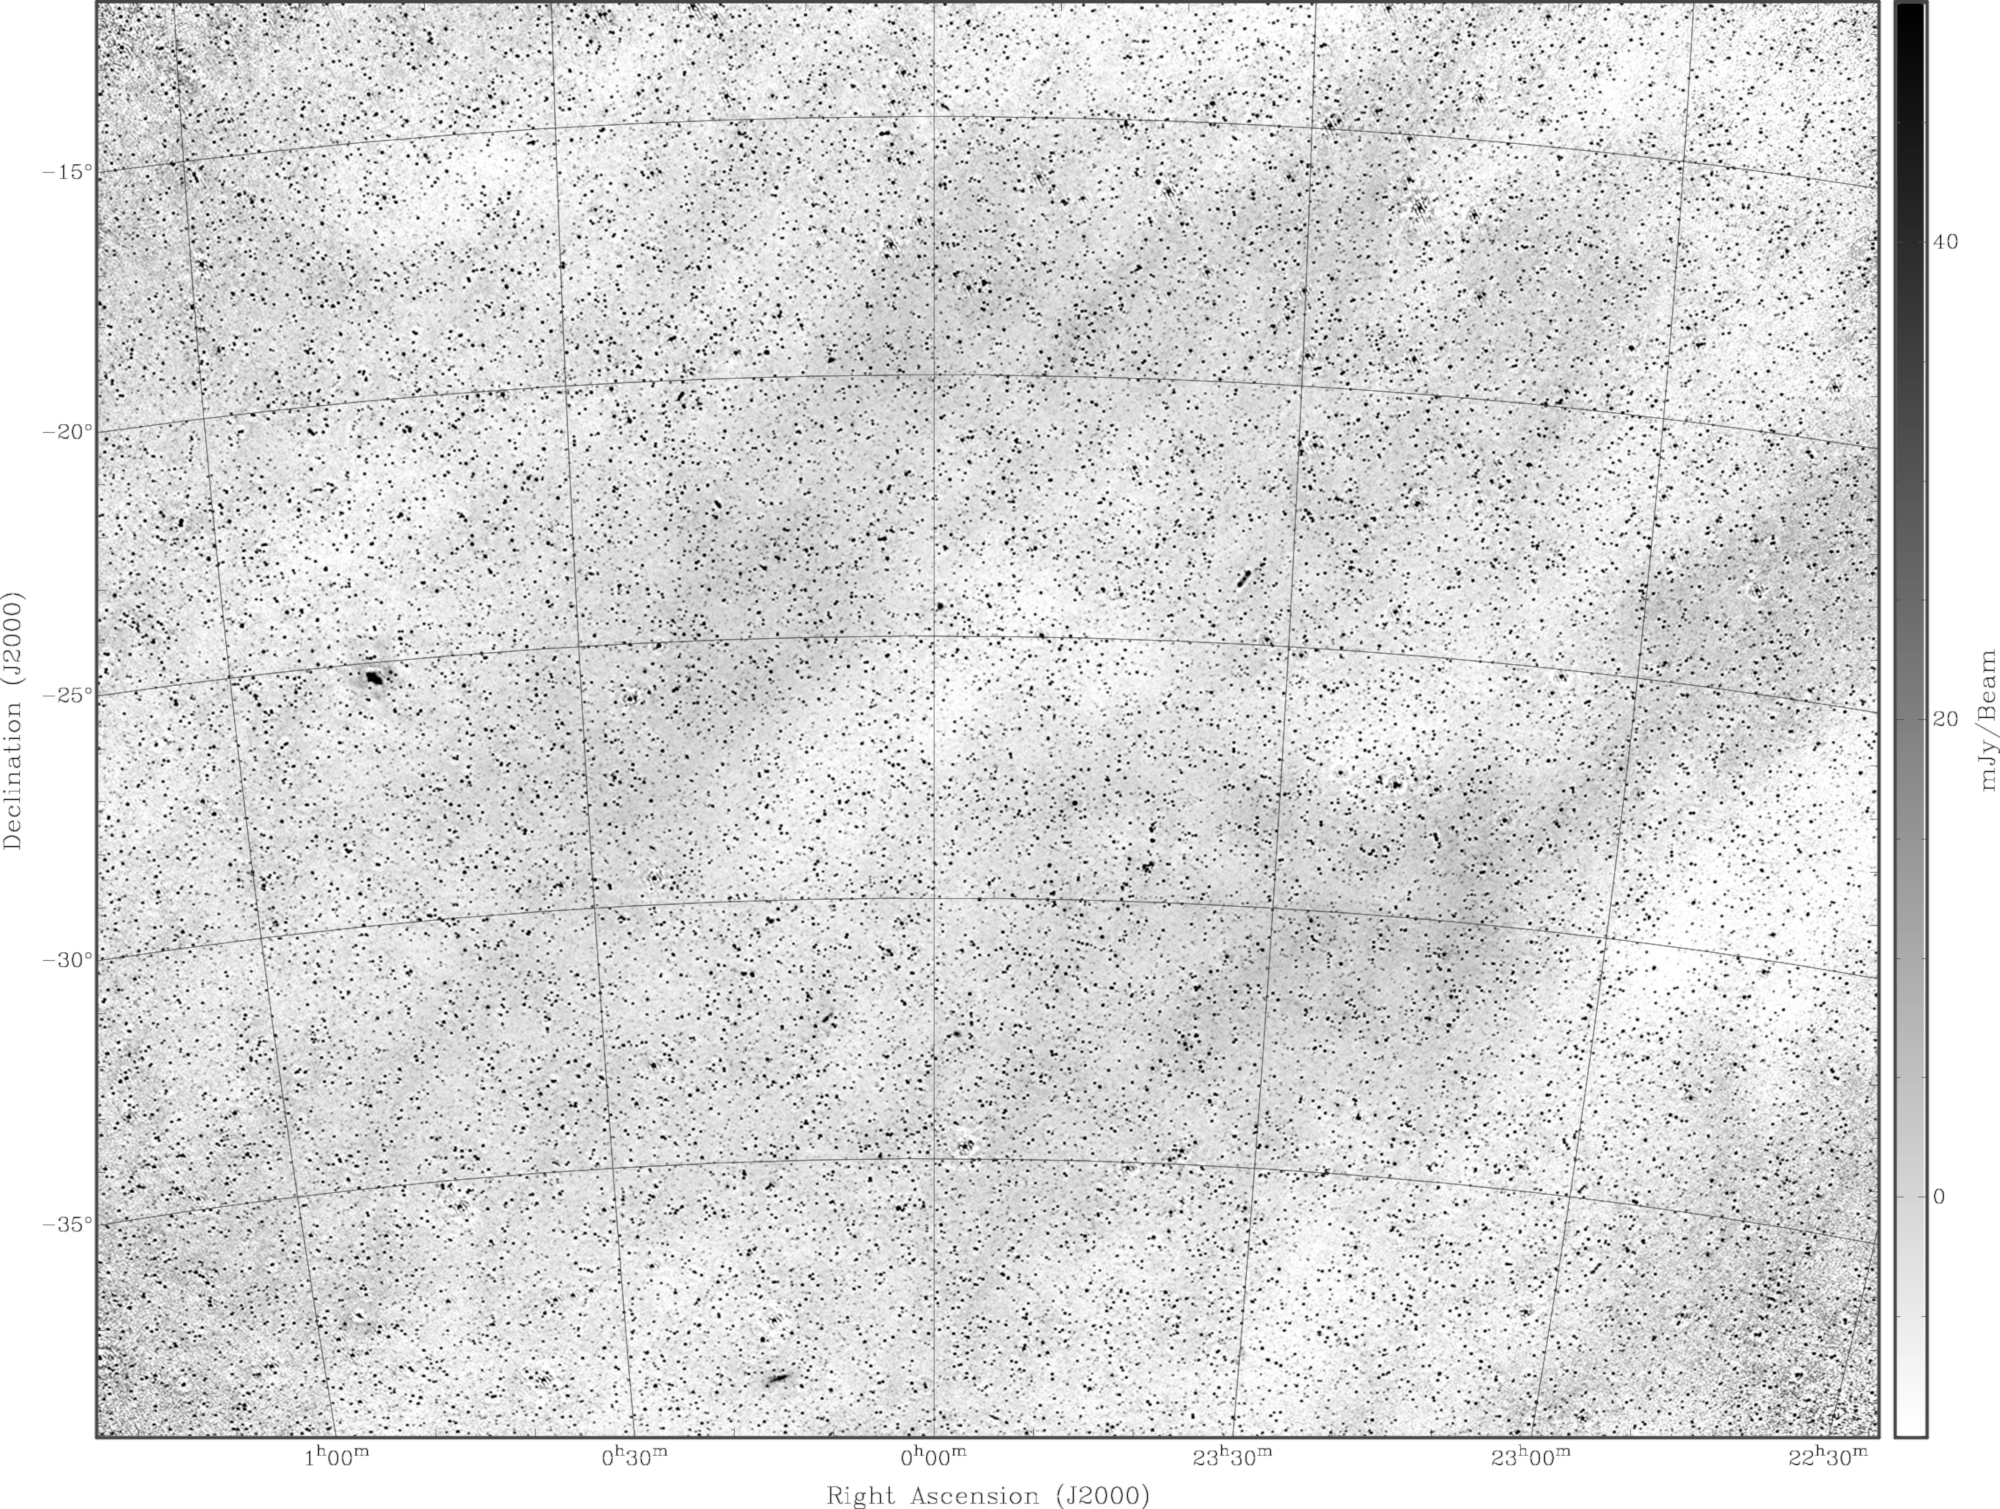
\includegraphics[width=\textwidth]{MWA-EoR0-fullbw}
  \bicaption[MWA 对 EoR0 天区的深度曝光图像]{%
    MWA 对 EoR0 天区 (R.A. = \SI{0}{\degree}, Dec.\@ = \SI{-27}{\degree})
    累计观测 \SI{45}{\hour} 获得的波束修正后的图像,大小约为 \SI{45 x 30}{\degree}.
  }{%
    The beam-corrected map of the EoR0 field
    (R.A. = \SI{0}{\degree}, Dec.\@ = \SI{-27}{\degree}) obtained by
    the MWA after \SI{45}{\hour} of integration time.
    The image size is about \SI{45 x 30}{\degree}.
    \\来源/Credit:
    \citeay{offringa2016}.
  }
  \label{fig:mwa-eor0}
\end{figure}

根据目前的观测证据和研究结果,可将河外点源大致分为两大类 \cite{padovani2016}:
\begin{itemize}
  \item \emph{射电星系 (radio galaxy)}:
    宿主通常为巨型椭圆星系 (elliptical galaxy),
    射电辐射结构远超出宿主星系本身的范围(如相对论性喷流),
    在 \SI{1.4}{\GHz} 处的射电功率 $\gtrsim$\,\SI{e22}{\watt\per\hertz}
    \cite{ledlow1996}.
    \citeay{fanaroff1974} 根据射电星系的功率和形态将其大致分为两小类:
    (1) \ac{fr} II 型:功率较强,具有射电瓣 (lobe) 以及显眼的\ac{hotspot};
    (2) \ac{fr} I 型:功率较弱,则具有相对弥散的射电羽 (plume).
    由此可见,很多点源其实具有复杂的形态结构,所以\enquote{点源}这一称法并不准确,
    主要是为了与下文 (\autoref{sec:eg-extended})
    将要介绍的\enquote{展源}区分开来.

  \item \emph{\ac{src-compact}}:
    没有明显的射电辐射结构,呈致密点状.
    根据射电辐射的来源,可主要分为
    恒星形成星系 (star-forming galaxy) \cite{condon1992}
    和\ac{agn} \cite{urry1995,antonucci1993,padovani2017}.
    同时 \ac{agn} 还可进一步分为\ac{quasar} \cite{barthel1989,antonucci1993}、
    \ac{blazar} \cite{giommi2012,giommi2013}、
    射电宁静 (radio-quiet) \ac{agn} \cite{sandage1965,wilson1995} 等子类.
\end{itemize}

目前的低频观测结果显示点源的频谱是光滑的,没有明显的谱线结构 \cite{offringa2016}.
但是不同类别的点源具有不同的谱指数和频谱形态.
还有小部分点源的辐射具有显著偏振,所以观测得到的频谱的光滑性会受到\ac{pl}的影响
\cite{geil2011,vanEck2018}.
此外,河外点源的成团效应 (clustering effect) 会改变其功率谱,
该效应需要被仔细考虑以获得准确的 EoR 信号功率谱
\cite{diMatteo2002,diMatteo2004,liu2011,alonso2015,murray2017}.

%---------------------------------------------------------------------
\subsection{河外展源}
\label{sec:eg-extended}

\ac{gc}由成百上千个成员星系、弥漫于成员星系之间的 \ac{icm} 以及暗物质组成
\cite{sarazin1986,bohringer2010}.
自 1959 年首次在 Coma 星系团中发现了尺度约 \SI{1}{Mpc} 的弥散射电辐射以来
\cite{large1959},
目前已在百来个星系团中探测到了弥散射电辐射 \cite{feretti2012,vanWeeren2019},
根据其尺度、形态、位置等特征,这些弥散射电源可大致分为以下三类
\cite{feretti2012,kale2016}:
\begin{itemize}
  \item \emph{\acf{rh}}:
    位于星系团的中央区域,尺度达 \si{\Mpc} 量级,形态比较规则,目前只发现于并合星系团中.
    如\autoref{fig:diffuse-emission} 左栏所示.
  \item \emph{\acf{rmh}}:
    位于弛豫冷核星系团的中央区域,通常围绕中央射电星系,尺度为数百 \si{\kpc},形态比较规则.
    如\autoref{fig:diffuse-emission} 中栏所示.
  \item \emph{\acf{rr}}:
    位于星系团的外围区域,尺度亦达 \si{\Mpc} 量级,呈长条不规则形态,辐射具有较强的偏振;
    在并合星系团和弛豫星系团均有发现,在若干星系团中成对出现.
    \autoref{fig:diffuse-emission} 右栏展示了一个双\ac{rr}的情形.
\end{itemize}
此外,在一些星系团中同时观测到了\ac{rh}和\ac{rr}.

\begin{figure}[htp]
  \centering
  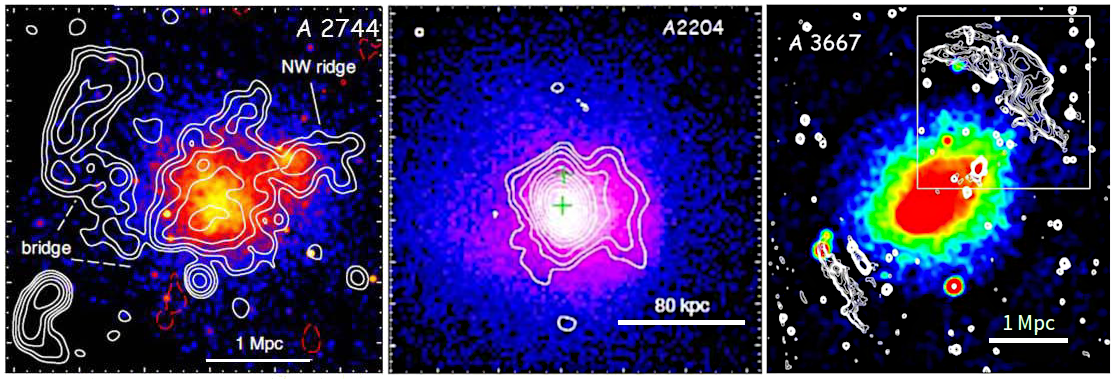
\includegraphics[width=\textwidth]{cluster-diffuse-emission}
  \bicaption[星系团的弥散射电辐射的典型样例]{%
    星系团的弥散射电辐射的典型样例:
    \uline{(左栏)} Abell 2744 中的\acs*{rh};
    \uline{(中栏)} Abell 2204 中的\acs*{rmh};
    \uline{(右栏)} Abell 3667 中的双\acs*{rr}.
    射电辐射以白色\ac{contour}\acuse{contour}标记,并叠加在 X 射线图像上.
  }{%
    Typical examples of diffuse radio emission in galaxy clusters:
    \emph{(left)} a radio halo in Abell 2744;
    \emph{(middle)} a radio mini-halo in Abell 2204;
    \emph{(right)} double radio relics in Abell 3667.
    The radio emissions are marked with white contours and
    superimposed on X-ray images.
    \\来源/Credit:
    \citeay{brunetti2014}.
  }
  \label{fig:diffuse-emission}
\end{figure}

在星系团中发现弥散射电辐射表明
\ac{icm} 除了包含由高温 ($\gtrsim$\,\SI{1}{\keV}) 等离子气体构成的热成分,
还存在一个由高能电子 (Lorentz 因子 $\acs{g} > \num{e3}$) 构成的非热成分.
这些高能电子弥散于整个星系团,在约 \si{\uG} 的微弱磁场中产生同步辐射,
形成上述大尺度\ac{src-extended}.
电子的能量越高,由于同步辐射以及对 \ac{cmb} 光子的逆 Compton 散射而损失能量的速率越快,
寿命也就越短.
因此,相比高频波段 ($\gtrsim$\,\SI{1}{\GHz}),
\ac{icm} 展源在数百 MHz 的低频波段更容易形成,而且具有更长的寿命.
以\ac{rh}为例,SKA1-Low 预计将发现约 2500 个 \cite{cassano2015},
远远超过目前已发现的总数(71 个已确认,另有 9 个候选;
详见\autoref{app:halos} 中的\autoref{tab:halos}).
尽管 \ac{icm} 展源相比银河系辐射和河外明亮点源来说比较微弱,
但考虑到该前景成分的尺度较大(若干角分)、形态结构复杂、数目较多等特点,
\ac{icm} 展源将在\ac{ps}的角分尺度上对 EoR 信号的测量产生严重干扰,
是一个待仔细研究的重要前景成分 \cite{diMatteo2004,gleser2008}.

除了\ac{gc},潜在的河外\ac{src-extended}还包括\ac{sc}和\ac{lsf}.
在这些宇宙大尺度结构里分布着温度约为 \SIrange{e5}{e7}{\kelvin} 的\ac{whim}
和强度约为 \SIrange{10}{100}{\nano\gauss} 的极微弱磁场 \cite{vazza2014}.
在物质落入这些宇宙大尺度结构的过程中、或者物质沿着大尺度结构流动形成星系团等结构时,
会产生 Mach 数 $\gtrsim$\,20 的强激波 \cite{ryu2003,skillman2008},
从而加速带电粒子并产生同步辐射 \cite{vazza2015}.
受限于当代射电望远镜的灵敏度,目前还没有获得这些大尺度结构的射电观测证据.
\ac{ska} 将有能力打破这个局面,
打开研究分布在\ac{sc}和\ac{lsf}的 \ac{whim} 的大门 \cite{vazza2015}.
另一方面,源自这些大尺度结构的射电辐射将如何影响 EoR 信号的探测,
亦是一个值得探讨的问题.


%=====================================================================
\section{前景处理方法}
\label{sec:fg-methods}

微弱的 EoR 信号被强烈的前景干扰所淹没是 EoR 探测实验所面临的最主要困难之一.
如何有效地解决这个前景污染难题,是成功探测 EoR 信号的关键.
尽管前景污染的强度高达 EoR 信号的 \numrange{4}{5} 个数量级,
但是幸运的是,各前景成分的频谱在本质上是光滑的,
而 EoR 信号的频谱反映了在宇宙不同红移处(即频率)中性氢的分布情况
\cite{diMatteo2002,oh2003,gnedin2004},
所以会随频率剧烈震荡.
利用这个关键区别,原则上可以将 EoR 信号从强烈的前景污染中分离出来.

近十余年来,已有一批方法被提出来用于尝试从前景污染中分离 EoR 信号.
根据处理前景的策略,可将这些方法大致分为两大类 \cite{chapman2015,chapman2016}:
\begin{itemize}
\item \emph{前景扣除法}:
在图像空间或 $uv$ 空间(即 Fourier 空间),
利用前景辐射和 EoR 信号两者明显不同的频谱特征,
对每个像素点沿频率维度(即视线方向)识别光滑的前景成分并扣除,从而分离出 EoR 信号.
根据对前景频谱的建模方式,这类方法可进一步分为两小类:
\begin{itemize}
  \item 参数化 (parametric) 方法:
    认为前景频谱可以由一个参数化模型(如低阶多项式)来描述,
    然后用此模型拟合前景频谱并扣除.
    这类方法主要包括多项式拟合法及其变种
    \cite{wang2006,jelic2008,liu2009fgrm,wang2013,bonaldi2015}.
  \item 非参数化 (non-parametric) 方法:
    不直接假定前景频谱应该符合某一特定参数化模型,
    而是充分利用前景辐射和 EoR 信号具有不同的频谱特征来实现两者的分离.
    典型的方法有 Wp 平滑法 \cite{harker2009}、
    \ac{ica} \cite{chapman2012}、
    \ac{gmca} \cite{chapman2013}、
    \ac{cwt} \cite{gu2013}.
\end{itemize}

%.......................................
\item \emph{前景回避法}:
在二维功率谱 $\ac{psD}(\kperp, \klos)$ 上,
频谱光滑的前景干扰将主要分布在 \klos{} 较小的区域.
尽管复杂的仪器效应和观测效应会导致前景污染被\enquote{泄漏}到 \klos{} \ac{mode}里,
占据二维功率谱的右下方一个楔形区域,但是左上方的区域仍然几乎未受前景污染的影响,
即 EoR 窗口(详见下文 \autoref{sec:eor-window}).
因此,\ac{fg-avd}法通过识别并避开二维功率谱上受到前景污染的区域,
从而实现提取 EoR 信号的目标.
近年来,该方法已得到了较多的关注和研究 \cite{thyagarajan2013,liu2014,liu2014ii,
  barry2016,beardsley2016,trott2016,patil2017}.

\end{itemize}

上述两类方法均有各自的优缺点.
\ac{fg-rm}法的优点是能够保留 EoR 信号的全部信息,
但缺点是可能无法准确扣除前景污染或者将部分 EoR 信号误认为前景而扣除,
导致结果出现一定的偏差.
\ac{fg-avd}法的优点是可以有效地避免前景污染对 EoR 探测结果产生的可能偏差,
而主要缺点便是损失了 EoR 信号在 EoR 窗口之外的信息,
牺牲了仪器的灵敏度和利用效率 \cite{pober2014}.
可进一步参见 \citeay{chapman2016} 及其所引文献.

当然,这两类前景处理方法并不冲突,在实际中可以结合使用,
比如先在图像空间或 $uv$ 空间扣除明显的前景污染,
再利用\ac{fg-avd}法在二维功率谱上提取 EoR 信号 \cite{datta2010}.


%=====================================================================
\section{EoR 窗口}
\label{sec:eor-window}

在二维功率谱 $\ac{psD}(\kperp, \klos)$ 上,
频谱光滑的前景干扰原则上只分布在 \klos{} 较小的区域.
但是没有仪器是理想的,一些仪器效应和观测效应会将
\kperp{} \ac{mode}里的功率\enquote{混合}到 \klos{} \ac{mode}里,
即\emph{\acf{mode-mixing}}效应,
并且 \klos{} 受影响的范围与 \kperp{} 的大小成正相关,
因此,前景污染将占据二维功率谱的右下方一个楔形区域,
即\emph{\acf{fg-wedge}},如\autoref{fig:eor-window} 所示.
这个现象最早由 \citeay{datta2010} 基于模拟数据研究亮点源对 EoR 探测的影响时发现,
目前已被多个实际观测证实
\cite{pober2013,dillon2014,dillon2015,beardsley2016,pober2016,patil2017},
还有一系列工作对此现象进行了解释和深入研究 \cite{morales2012,parsons2012,trott2012,
  vedantham2012,hazelton2013,thyagarajan2013,liu2014,liu2014ii,jacobs2016}.

\begin{figure}[htp]
  \centering
  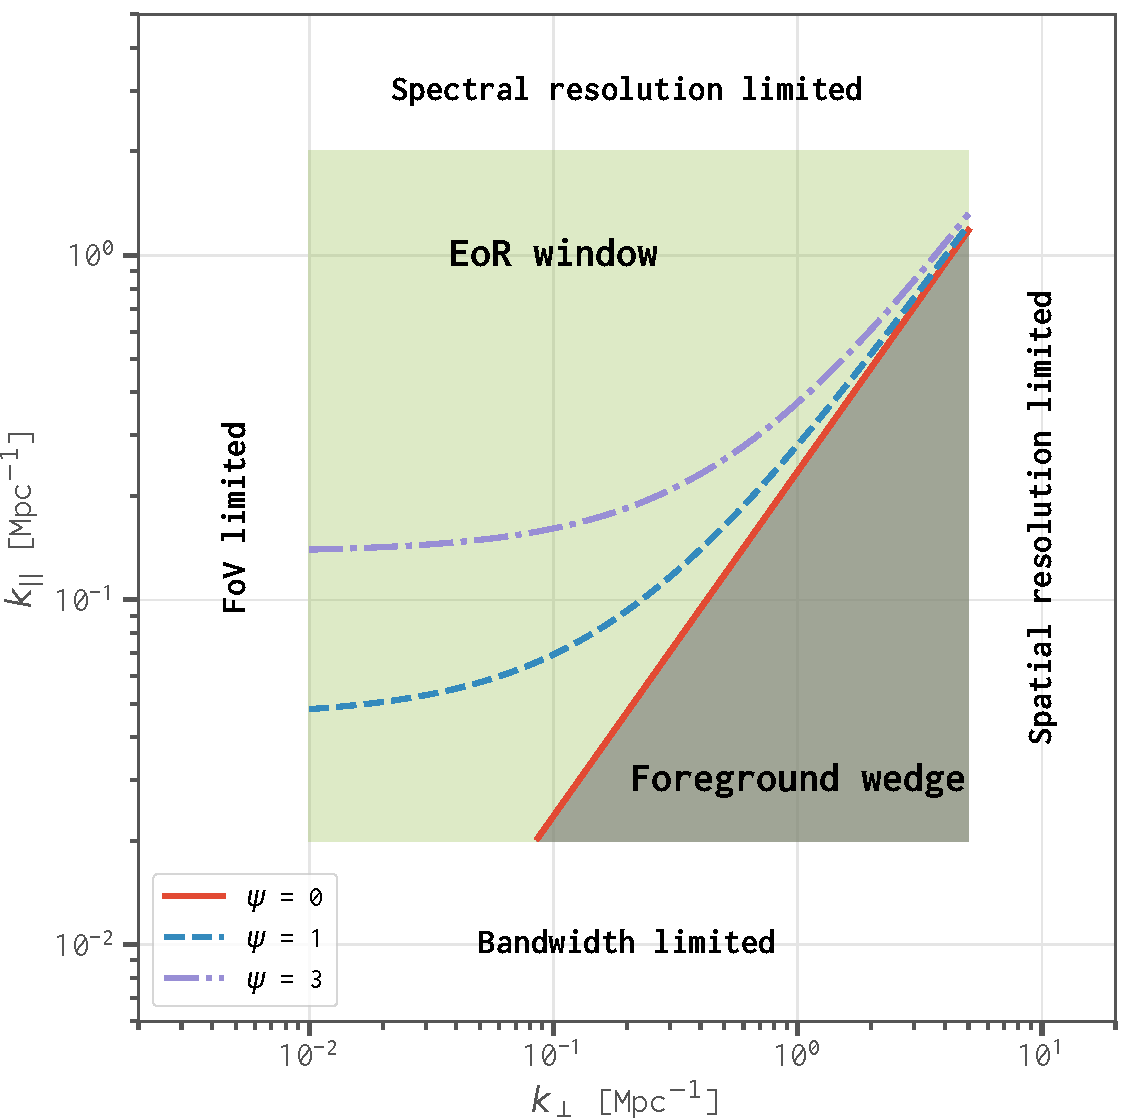
\includegraphics[width=0.9\textwidth]{EoR-window}
  \bicaption[EoR 窗口和前景楔形的示意图]{%
    二维功率谱 $\ac{psD}(\kperp, \klos)$ 上的 EoR 窗口(左上方绿色区域)
    和前景楔形(右下方灰色区域)的示意图.
    望远镜所能测量的二维功率谱的边界为:
    \kperp{} 的最小值和最大值分别由望远镜的视场大小和空间分辨率(对应于最长基线)决定、
    \klos{} 的最小值和最大值分别取决于频率带宽和频率分辨率.
    图中三条粗线显示了不同前景\acs*{spillover}程度
    [由\autoref{eq:eor-window} 中的 $w$ 描述]
    时的 EoR 窗口边界.
  }{%
    An illustration of the EoR window (green region in the upper left)
    and the foreground wedge (gray region in the bottom right) in the
    \ac{2d} power spectrum $\ac{psD}(\kperp, \klos)$.
    The boundaries of the \ac{2d} power spectrum that a telescope can
    measure are constrained by:
    the minimum and maximum \kperp{} are determined by the field of view
    (FoV) and the spatial resolution (corresponding to the longest
    baseline), respectively;
    the observing bandwidth and spectral resolution limit the minimum
    and maximum \klos, respectively.
    The bold lines show the EoR window boundaries corresponding to
    different foreground spillovers, described by the parameter $w$
    in Eq.~(\ref{eq:eor-window}).
  }
  \label{fig:eor-window}
\end{figure}

引起\ac{mode-mixing}的主要原因是干涉阵列固有的\ac{chromatic-effect},
即同一条\ac{baseline}的空间分辨率随着频率 $\nu$ 的增大而提高 \cite{liu2014}:
\begin{equation}
  \label{eq:baseline-u-nu}
  u = \frac{b}{\lambda}
    = \frac{b \nu}{\acs{speed-light}}
    \propto \kperp ,
\end{equation}
其中 $b$ 为\ac{baseline}的长度,
如\autoref{fig:chromatic-baselines} 所示.
\ac{mode-mixing}还可能由其他多种因素引起,比如:
干涉阵列的 \ac{psf} 随频率而变化 \cite{bowman2009,liu2009ps}、
前景模型不精确(如点源的强度或位置有偏差) \cite{datta2010,morales2012}、
仪器响应的校准不足 \cite{morales2012}、
不同\ac{baseline}的测量数据的叠加 \cite{hazelton2013}.
下文将基于干涉阵列的\ac{chromatic-effect},
简要介绍\ac{mode-mixing}的基本原理以及\ac{fg-wedge}的形成原因.
更严格的分析可参考 \citeay{liu2014} 和 \citeay{liu2014ii}.

\begin{figure}[htp]
  \centering
  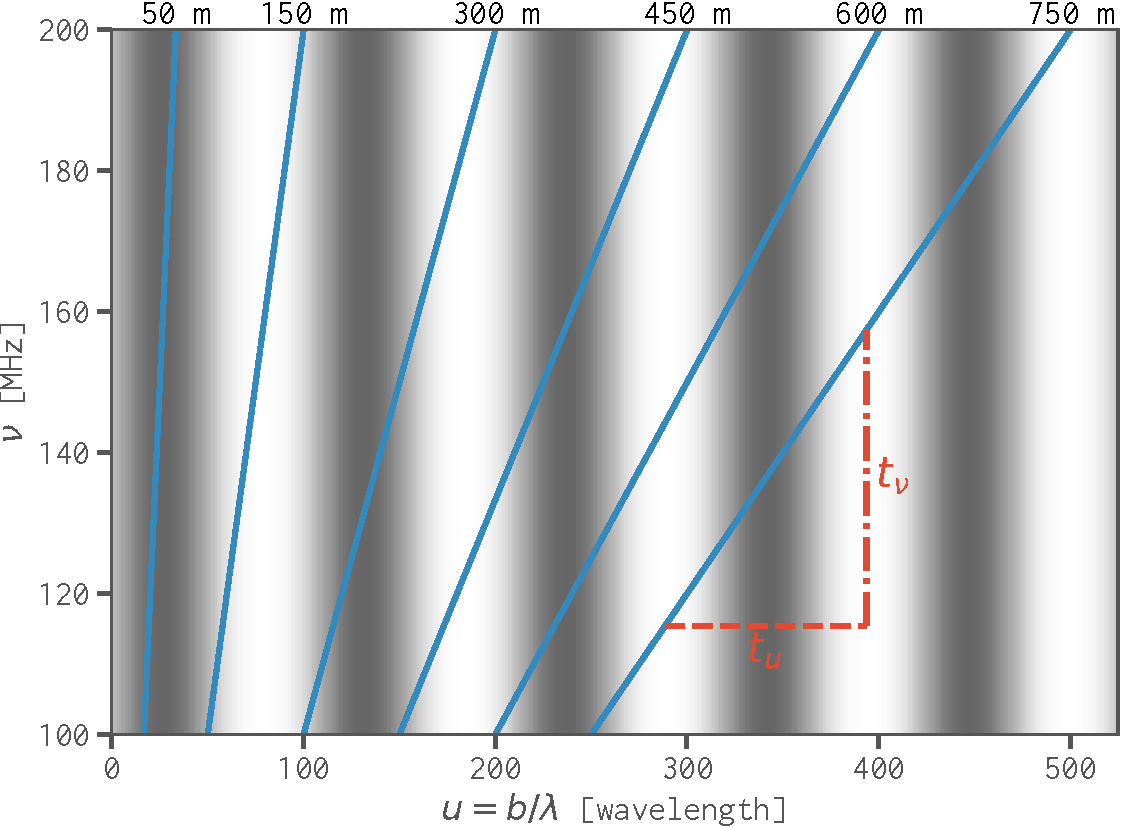
\includegraphics[width=0.8\textwidth]{chromatic-baselines}
  \bicaption[基线的\acs*{chromatic-effect}示意图]{%
    干涉阵列基线的\acs*{chromatic-effect}示意图.
    观测频率越高,同一条基线 $b$ 的空间分辨率越高,
    即所测量的波数 ($u = b / \lambda \propto \kperp$) 越大.
    同时,基线的长度越长,其空间分辨率的变化越显著,
    该基线的\acs*{chromatic-effect}也越明显(对应于图中的线越平).
  }{%
    An illustration of the chromatic effect of the interferometer baselines.
    As the observing frequency increases, the spatial resolution of
    one baseline $b$ also improves, i.e., the wavenumber
    ($u = b / \lambda \propto \kperp$) measured by the baseline
    increases.
    Meanwhile, the longer the baseline, the more significant the variation
    of its spatial resolution, i.e., its chromatic effect is more
    significant.
  }
  \label{fig:chromatic-baselines}
\end{figure}

考虑一个距离视场中心角度为 $\theta$ 的平谱点源(即各频率上的亮度相同),
可认为点源的坐标为 $(l, m) = (\sin\theta, 0)$.
根据\autoref{eq:vis-uv},该点源将在 $uv$ 平面产生一套条纹,可由下式描述:
\begin{equation}
  \acs{Vis}(u,v) \propto \exp [-2\Cpi\Ci\, (ul+vm)]
    = \exp (-2\Cpi\Ci\, u \sin\theta) ,
\end{equation}
可知条纹的间隔(或周期)为:
\begin{equation}
  \label{eq:ps-t-u}
  t_u = \frac{1}{\sin\theta} ,
\end{equation}
如\autoref{fig:chromatic-baselines} 中的背景条纹所示.
易知,点源偏离视场中心越远,所产生的条纹的间隔越窄.

尽管辐射源的亮度不随频率变化(即只有 \kperp{} \ac{mode}),
但是基线的\ac{chromatic-effect}导致观测的\ac{vis}数据将随频率涨落
(即出现了 \klos{} \ac{mode}),所以称为\ac{mode-mixing}.
再结合\autoref{eq:baseline-u-nu},
可知由\ac{mode-mixing}引起的涨落在频率维度的变化周期为 \cite{morales2012}:
\begin{equation}
  \label{eq:t-nu-u}
  t_{\nu} = \frac{\ac{speed-light}}{b} t_u
    = \frac{\nu}{u} t_u ,
\end{equation}
其中 $t_u$ 是信号在空间维度 $u$ 的变化周期 [\autoref{eq:ps-t-u}].
根据\autoref{eq:kperp-u} 和\autoref{eq:klos-eta} 可得:
\begin{align}
  t_{\nu} & = \frac{1}{\eta}
    = \frac{2\Cpi \nu \ac{Hz}}{\ac{speed-light} (1+z)} \frac{1}{\klos} , \\
  u & = \frac{\ac{D-comoving}(z)}{2\Cpi} \frac{1}{\kperp} ,
\end{align}
其中使用了 $\nu = \ac{freq21cm} / (1+z)$ 和 $\ac{Hz} = \ac{H0} \ac{Ez}$.
将上式以及\autoref{eq:ps-t-u} 代入\autoref{eq:t-nu-u},可得:
\begin{equation}
  \label{eq:klos-kperp}
  \klos = \frac{\ac{Hz} \ac{D-comoving}(z) \sin\theta}{
    \ac{speed-light} (1+z)} \kperp .
\end{equation}

\begin{figure}[htp]
  \centering
  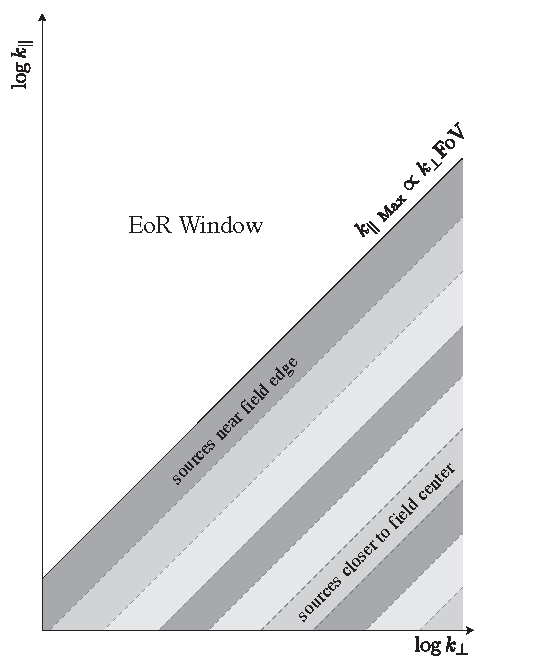
\includegraphics[width=0.7\textwidth]{foreground-wedge-fov}
  \bicaption[前景楔形和EoR 窗口的边界示意图]{%
    \acs*{fg-wedge}和EoR 窗口的边界示意图.
    距离视场中心越远的前景干扰源产生的污染区域越靠近左上方,
    因此望远镜的视场大小确定了\acs*{fg-wedge}的边界,
    左上方未受前景污染的区域则称为\enquote{EoR 窗口}.
  }{%
    The boundary between the foreground wedge and the EoR window.
    When the distance of a foreground souce from the field center increases,
    its contamination in the \ac{2d} power spectrum moves toward
    the upper-left regions.
    Therefore, the telescope's field of view determines the boundary of the
    foreground wedge, while the upper-left region that almost free from
    the foreground contamination is called the \enquote{EoR window}.
    \\来源/Credit:
    \citeay{morales2012}.
  }
  \label{fig:fg-wedge-fov}
\end{figure}

从上式可以清楚地看出,
视场内每一个前景干扰源(如未准确扣除的点源)在二维功率谱上产生的污染分布在右下方的一条斜线上;
\kperp{} 越大的\ac{mode}被混合到 \klos{} \ac{mode}的范围也越大,
于是形成\ac{fg-wedge},
如\autoref{fig:fg-wedge-fov} 所示.
另一方面,随着前景干扰源距离视场中心越来越远,其产生的污染区域也逐渐向左上方移动.
因此,视场内距离中心最远的干扰源(设该距离为 $\Phi$)确定了\ac{fg-wedge}的边界,
而左上方未受前景污染的区域则称为\emph{EoR 窗口},可表示为:
\begin{equation}
  \klos \ge \frac{\ac{Hz} \ac{D-comoving}(z) \sin\Phi}{
    \ac{speed-light} (1+z)} \kperp ,
\end{equation}
如\autoref{fig:fg-wedge-fov} 和\autoref{fig:eor-window} 所示.
干涉阵列通常具有明显的\ac{sidelobe},
因此\ac{fg-wedge}的具体范围(如 $\Phi$ 的大小)
与\ac{sidelobe}的行为密切相关.

在实际情况中,计算二维功率谱时只使用一个较窄的频带
(带宽 $\ac{bandwidth} \lesssim \SI{10}{\MHz}$) 以避免宇宙演化的影响,
所以计算过程中对频率维度进行 Fourier 变换时存在一定的边界效应.
另外,望远镜的频率响应也存在一些结构 \cite{deLeraAcedo2017,trott2017}.
这些因素将导致额外的前景\ac{spillover},使得\ac{fg-wedge}变大,
因此,\citeay{thyagarajan2013} 提出了如下改进的 EoR 窗口的边界表达式:
\begin{equation}
  \label{eq:eor-window}
  \klos \ge
    \frac{\ac{Hz} \ac{D-comoving}(z)}{\ac{speed-light} (1+z)}
    \left[ \kperp \sin\Phi
      + \frac{2\Cpi\ac{freq21cm} w}{(1+z) \ac{D-comoving}(z)
        \ac{bandwidth}} \right] ,
\end{equation}
其中 \ac{bandwidth} 为\acl{bandwidth},
$w$ 描述了前景\ac{spillover}的程度.
\autoref{fig:eor-window} 显示了 $w = 0, 1, 3$ 所对应的 EoR 窗口边界.


%=====================================================================
\section{小结}

TODO


%% EOF

%%
%% Copyright (c) 2018-2019 Weitian LI <liweitianux@sjtu.edu.cn>
%% Creative Commons BY 4.0
%%

\acuse{colorbar}

\chapter{低频射电天空的模拟}
\label{chap:simulation}

Based on our previous works \cite{wang2010,wang2013}, we have developed the
\href{https://github.com/liweitianux/fg21sim}{\texttt{FG21sim}}\footnote{%
  FG21sim: \url{https://github.com/liweitianux/fg21sim}}
software to simulate the low-frequency
radio sky by taking into account the contributions of our Galaxy,
extragalactic point sources, and radio halos in galaxy clusters.
We choose three representative frequency bands, namely
\numrange{120}{128}, \numrange{154}{162}, and \numrange{192}{200}
\si{\MHz}, and perform simulations for a sky patch of size
\SI{10 x 10}{\degree}.
The \SI{8}{\MHz} bandwidth is chosen to limit the effect of
cosmological evolution of the EoR signal when calculating power
spectra \cite{wyithe2004,thyagarajan2013}.
The simulated sky maps are pixelized into \num{1800 x 1800} with a pixel
size of \SI{20}{\arcsecond}.
The simulation parameters are also listed in \autoref{tab:freq-bands}.

\begin{table}[htp]
  \centering
  \bicaption{%
    三个频段的模拟参数
  }{%
    Simulation Parameters for the Three Bands
  }
  \label{tab:freq-bands}

  \begin{tabular}{cccc}
    \toprule
    频段 &
      \SIrange{120}{128}{\MHz} &
      \SIrange{154}{162}{\MHz} &
      \SIrange{192}{200}{\MHz} \\
    \midrule
    中心频率 ($\nu_c$) & \SI{124}{\MHz} & \SI{158}{\MHz} & \SI{196}{\MHz} \\
    EoR 红移范围 &
      \numrange{10.10}{10.84} &
      \numrange{7.77}{8.22} &
      \numrange{6.10}{6.40} \\
    带宽 (\ac{bandwidth}) & \multicolumn{3}{c}{\SI{8}{\MHz}} \\
    天区大小 & \multicolumn{3}{c}{\SI{10 x 10}{\degree}} \\
    图像大小 & \multicolumn{3}{c}{\num{1800 x 1800}} \\
    像素大小 & \multicolumn{3}{c}{\SI{20}{\arcsecond}} \\
    \bottomrule
  \end{tabular}
\end{table}

TODO:
We first elaborate the simulation of radio halos.
Following our previous work \cite{wang2010}, we have also simulated
several other foreground components, including the Galactic synchrotron
and free-free emissions as well as the extragalactic point sources,
in order to carry out comparisons of power spectra between radio halos
and other foreground components as an effort to better characterize the
contribution of radio halos to the low-frequency radio sky.


%=====================================================================
\section{星系团射电晕}
\label{sec:radio-halos}

TODO: Turbulence; Alfven, slow, fast modes; particle acceleration:
Lazarian et al. 2012, SSRv;
Petrosian 2012, SSRv.

截至目前,只有少量几个工作在研究 EoR 前景时考虑了\ac{gc}\ac{rh}
\cite{diMatteo2004,gleser2008,jelic2008},
而且对\ac{rh}的建模过于简化,比如
直接使用在低流量端很不完备的 \SI{1.4}{\GHz} \ac{fluxfunc} \cite{gleser2008}、
采用弥散很大的射电--X 射线标度关系 \cite{jelic2008}、
假定相同的频谱指数和均匀的表面亮度分布 \cite{gleser2008,jelic2008}.

为了更加有效地评估\ac{rh}对 EoR 探测的具体影响,
有必要努力改进对\ac{rh}的建模,获得更加逼真的\ac{rh}的图像和频谱信息.
为此,我们之前的一项工作\cite{wang2010}考虑了高能电子的能量损失过程,
改进了\ac{rh}的频谱特征的模拟.
在此基础上,本工作采用了一种半解析方法考虑了\ac{rh}的形成和演化过程,
进一步显著改进了\ac{rh}的建模.
对于一个\ac{gc},
首先根据\uline{扩展 Press--Schechter 理论} (extended Press--Schechter theory)
模拟其并合历史 (\autoref{sec:merging-history}),
运用\ac{turbreacc-model}来计算并合所产生的\ac{turbulence}对
\ac{icm} 中高能电子的再加速过程 (\autoref{sec:halo-evo}),
获得高能电子的能谱以及\ac{rh}的频谱随时间的演化,
从而得到所形成的\ac{rh}的性质 (\autoref{sec:halo-size})
并生成相应的图像 (\autoref{sec:halo-maps}).

Enrico Fermi 最早在 1949 年提出\ac{mfluid}中的带电粒子
可与其中的\ac{turbulence}发生随机散射而获得能量被加速,
并用来解释高能\ac{cr}的起源 \cite{fermi1949,fermi1954,davis1956},
这一加速机制被称为\emph{二阶 Fermi 加速}.
\ac{gc} \ac{icm} 主要包含 $\gtrsim \SI{1}{\keV}$ 的高温等离子气体,
同时还存在约 \si{\uG} 的磁场 \cite{govoni2004,ryu2008},所以是一个\ac{mfluid}.
为了解释\ac{rh}的性质(如尺度达 $\sim\si{Mpc}$、只在并合星系团中发现)和形成机制,
\citeay{brunetti2001} 和 \citeay{petrosian2001}
首先将二阶 Fermi 加速机制应用于\ac{gc} \ac{icm},
认为并合会产生大规模的\ac{turbulence},
在\enquote{当地}加速 \ac{icm} 中的相对论性电子,
从而产生弥散的同步辐射,形成大尺度的\ac{rh}.
这就是\emph{\ac{turbreacc-model}}.
该模型在诸多后续研究中得到了充分的发展和改进
\cite{fujita2003,brunetti2004,cassano2005,brunetti2007,brunetti2011},
是目前解释\ac{rh}的主流模型.
详见 \citeay{brunetti2014} 综述文.
下文将详细介绍\ac{rh}的建模方法和结果.

%---------------------------------------------------------------------
\subsection{质量函数}
\label{sec:mass-function}

现在普遍认为,宇宙目前的结构是由极早期的微小密度扰动发展而来的 \cite{peebles1980}.
根据\acf{cdm} 模型,\ac{cdm} 粒子的速度弥散很小,因此有利于先形成小尺度结构;
然后在引力和宇宙膨胀的共同作用下,逐步形成尺度越来越大的结构
\cite{davis1985,bond1991,lacey1993}.
这就是\emph{\acf{hier-clustering}}模型.

当密度扰动进行非线性增长阶段,其计算变得非常复杂而主要依赖于数值模拟.
\ac{spherical-collapse}模型可作为一个简单的解析近似得到与数值模拟相近的结果
\cite{gunn1972}.
根据该模型,暗物质坍缩形成暗物质晕,然后重子物质被暗物质晕的引力\ac{accretion},
在晕中沉积并演化为星系、星系团等结构.
利用该模型,\citeay{press1974} 从密度扰动的随机统计性质推导出了暗物质晕
(即星系、星系团等结构)的数目随质量的分布及其时间演化,
即 \emph{Press-Schechter 质量函数}.
因此,在红移 $z$ 处,每单位\ac{V-comoving}内质量范围为 $[M,\, M+\R{d}M]$
的\ac{gc}的数目 \ac{n-cl} 为:
\begin{equation}
  \label{eq:ps-mass-func}
  \ac{n-cl} \,\D{M} =
    \sqrt{\frac{2}{\Cpi}} \frac{\langle \rho_0 \rangle}{M}
    \frac{\delta_c(z)}{\sigma^2(M)} \left| \diff{\sigma(M)}{M} \right|
    \exp\!\left[ -\frac{\delta_c^2(z)}{2\sigma^2(M)} \right] \,\D{M} ,
\end{equation}
其中
$M$ 是星系团的质量,
$\langle \rho_0 \rangle$ 是当前的宇宙平均密度,
$\delta_c(z)$ 是暗物质坍缩形成暗物质晕的\acl{delta-crit}
(critical linear overdensity) [见\autoref{eq:delta-crit}],
$\sigma(M)$ 是当前在平均质量为 $M$ 的球形区域里的密度涨落的\ac{rms}值.

在星系团的质量范围内,上式中的密度涨落 $\sigma(M)$ 可合理地近似为以下幂律形式
\cite{sarazin2002,randall2002}:
\begin{equation}
  \label{eq:sigma-mass}
  \sigma(M) = \ac{sigma8} \left( \frac{M}{M_8} \right)^{-\alpha} ,
\end{equation}
其中
\ac{sigma8} 是\acl{sigma8},
$M_8$ 是半径为 \SI{8}{\per\hubble\Mpc} 的球形区域里的质量:
\begin{equation}
  M_8 = \frac{4\Cpi \langle \rho_0 \rangle}{3}
    (\SI{8}{\per\hubble\Mpc})^3 ,
\end{equation}
以及指数 $\alpha = (n+3)/6$ 并且有 $n = -7/5$ \cite{bahcall1998}.

将星系团的质量下限设为 $M_{\R{min}} = \SI{2e14}{\solarmass}$
以及红移上限设为 $z_{\R{max}} = 4$,
于是由 Press--Schechter 质量函数 [\autoref{eq:ps-mass-func}]
可计算出 \SI{10 x 10}{\degree} 的天区内的星系团总数为 504,
以及相应的质量和红移分布(如\autoref{fig:m-z-dist} 所示).
接着,对质量和红移分布随机采样,得到一系列 $(M_{\R{sim}}, z_{\R{sim}})$ 对,
于是构建成所需的星系团样本.

\begin{figure}[htp]
  \centering
  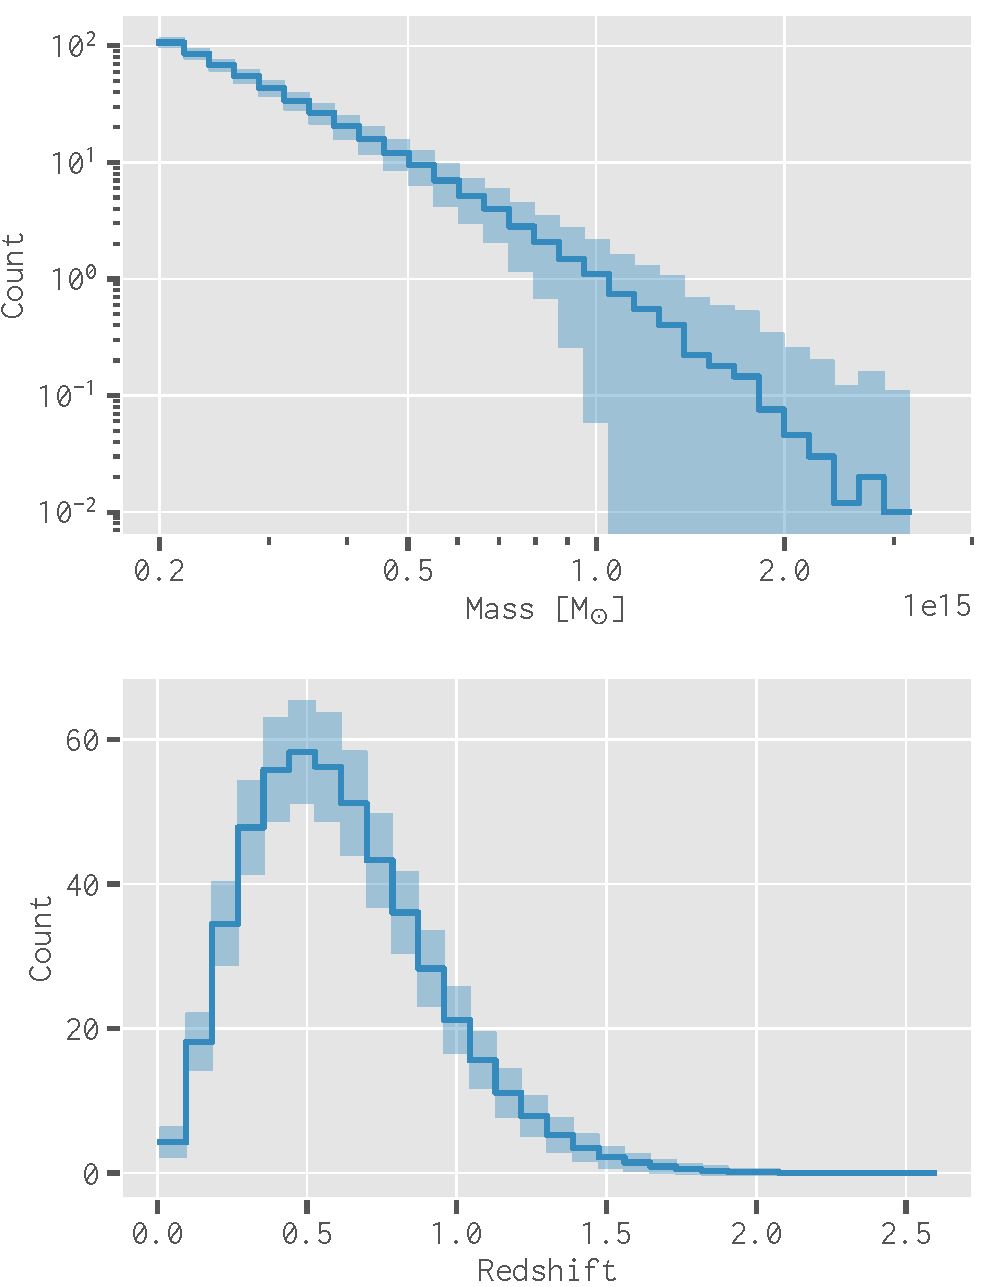
\includegraphics[width=0.8\textwidth]{mass-z-dist}
  \bicaption[星系团的红移和质量分布直方图]{%
    在 \SI{10 x 10}{\degree} 的天区内,星系团的红移(上栏)和质量(下栏)分布直方图.
    其中的实线和阴影区域分别表示 500 次模拟的平均值和 68\% 误差范围.
  }{%
    The mass (upper panel) and redshift (lower panel) histograms of the
    simulated galaxy clusters in a \SI{10 x 10}{\degree} sky patch.
    The solid lines and shaded regions represent the means and
    68\% uncertainties derived from 500 simulation runs,
    respectively.
  }
  \label{fig:m-z-dist}
\end{figure}

%---------------------------------------------------------------------
\subsection{并合历史}
\label{sec:merging-history}

上述 Press--Schechter 质量函数只给出了在不同红移处宇宙中的\ac{gc}的质量分布,
没有提供单个星系团的形成历史.
这个问题由 \citeay{lacey1993} 通过对 Press--Schechter
理论进行了扩展而给出了解决方案.
给定一个星系团,\uline{扩展 Press--Schechter 理论}描述了其\ac{progenitor}的质量分布,
然后利用 Monte Carlo 模拟便可构建出该星系团的成长历史,即\emph{\acf{m-tree}}
\cite{lacey1993,randall2002}.

设一个星系团在 $t_1$ 时刻的质量为 $M_1$,经过一次成长步骤(并合或\ac{accretion})后,
其质量在 $t_2$ ($> t_1$) 时刻增长为 $M_2$.
给定 $M_2$ 和 $t_2$,扩展 Press--Schechter 理论给出了该星系团在一个较早时刻 $t_1$
具有一个质量范围为 $[M_1,\, M_1+\D{M_1}]$ 的\ac{progenitor}的\ac{pr-cond}为
\cite{lacey1993,randall2002}:
\begin{equation}
  \label{eq:eps-condprob}
  \R{Pr}(M_1, t_1 \,|\, M_2, t_2) \,\D{M_1} =
    \frac{1}{\sqrt{2\Cpi}} \frac{M_2}{M_1}
    \frac{\delta_{c1} - \delta_{c2}}{(\sigma_1^2 - \sigma_2^2)^{3/2}}
    \left| \diff{\sigma_1^2}{M_1} \right|
    \exp \!\left[ -\frac{(\delta_{c1} - \delta_{c2})^2}
      {2(\sigma_1^2 - \sigma_2^2)} \right] \,\D{M_1} ,
\end{equation}
其中
$\delta_{ci} \equiv \delta_c(t_i)$,$\sigma_i \equiv \sigma(M_i)$,
同时下标 $i = 1, 2$ 分别表示这些参数在时刻 $t_1$ 和 $t_2$ 的值.
进一步定义 $\psi \equiv \sigma^2(M)$ 和 $\omega \equiv \delta_c(t)$,
上式可简化为:
\begin{equation}
  \label{eq:eps-condprob2}
  \R{Pr}(\Delta\psi, \Delta\omega) \,\D{\Delta\psi} =
    \frac{1}{\sqrt{2\Cpi}} \frac{\Delta\omega}{(\Delta\psi)^{3/2}}
    \exp \!\left[ -\frac{(\Delta\omega)^2}{2 \Delta\psi} \right]
    \,\D{\Delta\psi} ,
\end{equation}
其中
$\Delta\psi = \sigma_1^2 - \sigma_2^2$,
$\Delta\omega = \delta_{c1} - \delta_{c2}$.
注意 $\psi$ 随 $M$ 的增大而单调递减,$\omega$ 亦随 $t$ 的增大而单调递减.

对于样本 (\autoref{sec:mass-function}) 中的每一个星系团,为了模拟其\ac{m-tree},
我们从\enquote{当前的}质量 $M_{\R{sim}}$ 和红移 $z_{\R{sim}}$ 出发,
运用 Monte Carlo 方法逐步追溯其成长历史,时间步长为 $\Delta\omega$.
为了能够分辨质量变化为 $\Delta M_c$ ($\ll M_2$) 的并合,
时间步长 $\Delta\omega$ 应满足 \cite{lacey1993}:
\begin{equation}
  \Delta\omega \lesssim (\Delta\omega)_{\R{max}} =
    \left[ \psi \left| \diff{\ln \sigma^2}{\ln M_2} \right|
      \left( \frac{\Delta M_c}{M_2} \right) \right]^{1/2} .
\end{equation}
本工作采用了自适应的时间步长 \cite{randall2002}:
$\Delta\omega = (\Delta\omega)_{\R{max}} \big/ 2$.

在追溯的每一步,当确定时间步长 $\Delta\omega$ 后,
则并入星系团的质量(由 $\Delta\psi$ 描述)的\ac{cdf}为:
\begin{align}
  F_{\Delta\psi}(<\!\Delta\psi, \Delta\omega)
    & = \int_0^{\Delta\psi} \R{Pr}(\Delta\psi', \Delta\omega)
      \,\D{\Delta\psi'} \\
    & = 1 - \erf \left( \frac{\Delta\omega}{\sqrt{2\Delta\psi}} \right) ,
  \label{eq:cdf-submass}
\end{align}
其中 $\erf(\cdot)$ 为\ac{errfunc}:
\begin{equation}
  \erf(x) = \frac{2}{\sqrt{\pi}} \int_0^x \Ce^{-t^2} \,\D{t} .
\end{equation}
对\autoref{eq:cdf-submass} 随机采样得到一个 $\Delta\psi$,
于是,星系团 $M_2$ 的一个\ac{progenitor}的质量 $M_1$
由 $\psi_1 = \psi_2 + \Delta\psi$ 确定 [参见\autoref{eq:sigma-mass}],
同时另一个\ac{progenitor}的质量为 $\Delta M = M_2 - M_1$.

设 $M_m \equiv \max(M_1, \Delta M)$ 和 $M_s \equiv \min(M_1, \Delta M)$
分别为并合的主星系团(简称\emph{主团})和子星系团(简称\emph{子团}),
如果 $M_s > \Delta M_c$,则认为发生了一次并合事件,否则认为是\ac{accretion}过程
\cite{randall2002}.
目前普遍认为可观测到的\ac{rh}与最近(在观测者的参考系)发生的\ac{m-major}相关联,
而且\ac{rh}的典型寿命较短,比如在 \SI{1.4}{\GHz} 的寿命
$\tau_{\R{halo}} \lesssim \SI{1}{\Gyr}$ \cite{brunetti2009,cassano2016}.
因此,本文采用 $\Delta M_c = \SI{e13}{\solarmass}$ \cite{cassano2005},
并且只针对主团从\enquote{当前}时刻 $t_{\R{sim}}$ (对应于 $z_{\R{sim}}$)
追溯 $t_{\R{back}} = \SI{3}{\Gyr}$.
于是,获得每个星系团的并合历史
$\left\{\left( M_m^{(i)}, M_s^{(i)}, t_{\R{merger}}^{(i)} \right)\right\}$
用于开展后续射电晕的模拟.

星系团的并合历史(即\ac{m-tree})是随机模拟的.
以一个质量为 \SI{e15}{\solarmass} 的星系团为例,重复模拟其\ac{m-tree} 30 次,
可得到 30 颗不同的\ac{m-tree},如\autoref{fig:merging-history} 上栏所示.
同时,该图下栏显示了从 \autoref{sec:mass-function} 样本中随机挑选的 30 个星系团
的\ac{m-tree},其中每个星系团只随机生成了一颗\ac{m-tree}.

\begin{figure}[htp]
  \centering
  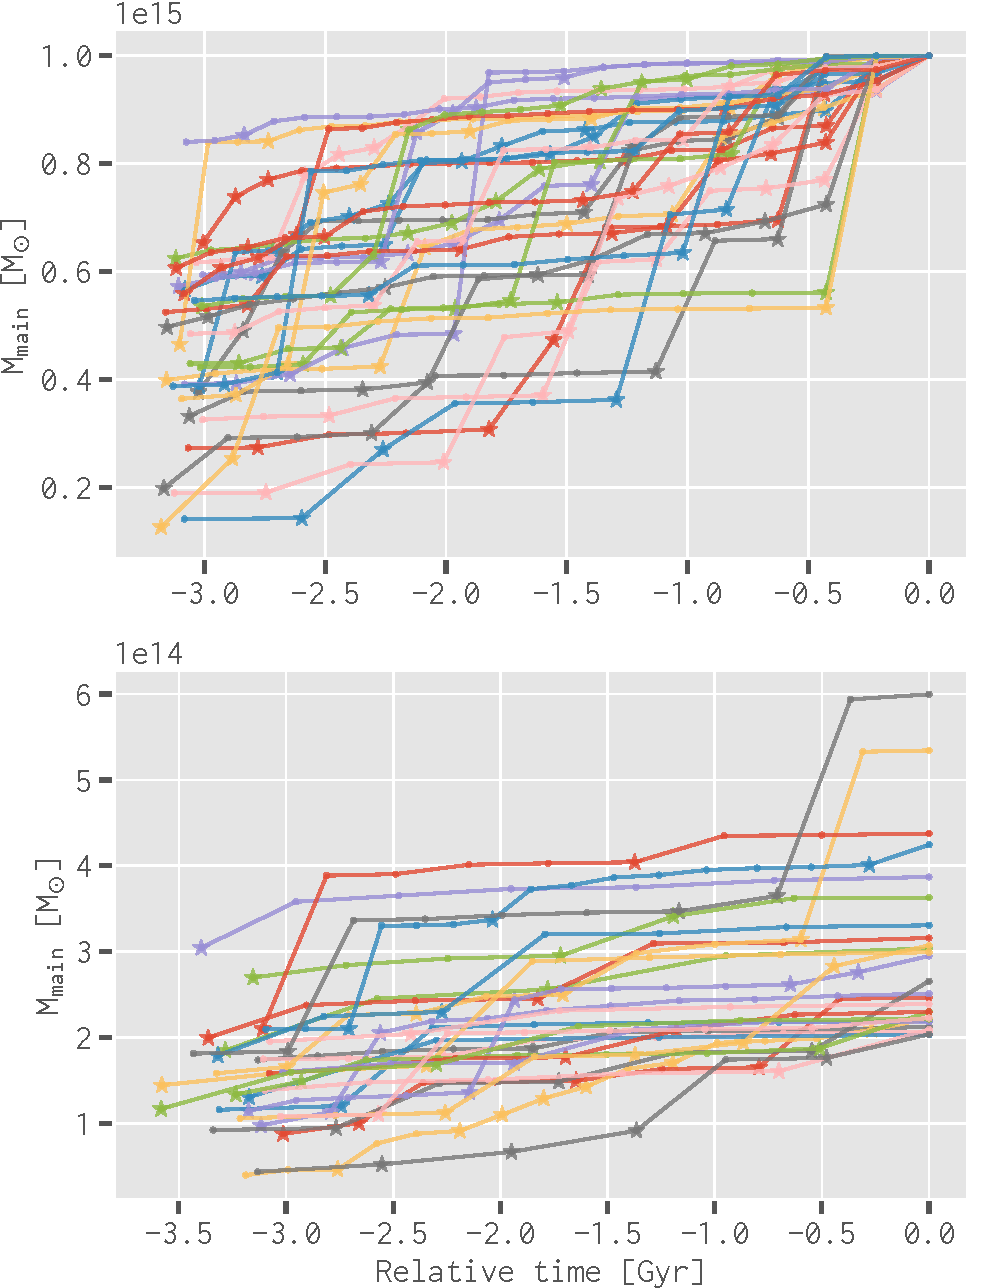
\includegraphics[width=0.8\textwidth]{merging-history}
  \bicaption[星系团并合树的模拟结果示例]{%
    \uline{(上栏)}
    对同一个质量为 \SI{e15}{\solarmass} 的星系团,重复模拟其\acs*{m-tree} 30 次
    所得到的 30 颗不同的\acs*{m-tree}.
    \uline{(下栏)}
    从 \autoref{sec:mass-function} 样本中随机挑选 30 个星系团,
    对每个星系团随机模拟一颗\acs*{m-tree}.
    星号和细点分别表示并合和\acs*{accretion}事件.
  }{%
    \textbf{(Upper)} Merger trees for one galaxy cluster of mass
    \SI{e15}{\solarmass} obtained by repeating the random build process
    for 30 times.
    \textbf{(Lower)} Example merger trees for 30 galaxy clusters randomly
    drawn from the sample constructed in \autoref{sec:mass-function}.
    Asterisks mark merger events and dots represent accretion events.
  }
  \label{fig:merging-history}
\end{figure}

%---------------------------------------------------------------------
\subsection{演化模型}
\label{sec:halo-evo}

根据\ac{turbreacc-model},星系团 \ac{icm} 里充满一群非热的\ac{e-primary},
这些电子可在多种过程中产生并被注入到 \ac{icm} 中,比如 \ac{agn} 活动、恒星形成,
详见 \citeay{blasi2007} 和 \citeay{brunetti2014} 综述文.
当星系团经历\ac{m-major}时,整个 \ac{icm} 中都将产生剧烈的\ac{turbulence},
就地加速\ac{e-primary}至极高的能量 ($\ac{g} > \num{e3}$),
从而形成弥散的\ac{rh}.
在另一方面,多种机制会使这些高能电子损失能量 \cite{sarazin1999},其中包括:
产生\ac{rad-syn}、与 \ac{cmb} 光子发生逆 Compton 散射、
与 \ac{icm} 中的离子发生 Coulomb 碰撞.

对于一群能量分布各向同性的电子,在上述加速和能量损失的共同作用,
其能谱 \ac{n-e} 随时间的演化由以下 Fokker--Planck 方程描述
\cite{eilek1991,schlickeiser2002}:
\begin{equation}
  \label{eq:fokkerplanck}
  \pdiff{\ac{n-e}}{t} =
    \pdiff{}{\ac{g}} \left[ \ac{n-e} \left(
      \left| \diff{\ac{g}}{t} \right| -
      \frac{2}{\ac{g}} \ac{coef-diffusion}(\ac{g}, t) \right) \right]
    + \pdiff{}{\ac{g}} \left[
      \ac{coef-diffusion} \pdiff{\ac{n-e}}{\ac{g}} \right]
    + \ac{e-inj}(\ac{g}, t) ,
\end{equation}
其中
\ac{g} 是电子的 \acl{g},
\ac{coef-diffusion} 是描述\ac{turbulence}和电子相对作用的\acl{coef-diffusion},
$|\R{d}\gamma / \R{d}t|$ 是电子的能量损失速率,
还有 \ac{e-inj} 描述了电子的注入过程.

%.....................................................................
\subsubsection{热成分的性质}

对于星系团 \ac{icm} 的热成分,其中的热电子的数密度 (number density) \ac{n-th} 为:
\begin{equation}
  \label{eq:n-th}
  \ac{n-th} \simeq
    \frac{3 \ac{f-gas} \ac{M-vir}}{
      4\Cpi \ac{mol-weight-m} \ac{mass-u} \,r^3_{\R{vir}}} ,
\end{equation}
其中
$\ac{mol-weight-m} \simeq 0.6$ 是 \ac{icm} 的\acl{mol-weight-m}
(mean molecular weight) \cite{ettori2013},
\ac{mass-u} 是\acl{mass-u} (atomic mass unit),
\ac{M-vir} 是星系团的\acl{M-vir} (virial mass),
\ac{r-vir} 是其\acl{r-vir} (virial radius)
[参见\autoref{eq:radius-virial}],
以及 $\ac{f-gas} \simeq \ac{Ob0}/\ac{Om0}$
是星系团中的气体占总质量 (\ac{M-vir}) 的比例.

相应地,\ac{icm} 的热能密度 (thermal energy density) \ac{e-th} 由下式给出:
\begin{equation}
  \label{eq:e-th}
  \ac{e-th} = \frac{3}{2} \,\ac{n-th} \ac{kb} \ac{T-cl} ,
\end{equation}
其中 \ac{icm} 的平均温度 \ac{T-cl} 可近似为 \cite{cavaliere1998}:
\begin{equation}
  \label{eq:t-icm}
  \ac{T-cl} \simeq \ac{T-vir} + \frac{3}{2} \,T_{\R{out}} ,
\end{equation}
其中 \ac{T-vir} 为星系团的\acl{T-vir} (virial temperature):
\begin{equation}
  \ac{T-vir} =
    \frac{\ac{mol-weight-m} \ac{mass-u} \ac{G} \ac{M-vir}}{2\,\ac{r-vir}} ,
\end{equation}
以及 $T_{\R{out}} \simeq \SI{0.5}{\keV}$
是从星系团外围区域 ($\gtrsim \ac{r-vir}$) 流入的气体的温度 \cite{fujita2003}.

%.....................................................................
\subsubsection{电子注入过程}

星系团及其成员星系中持续发生着 \ac{agn} 活动、恒星形成等过程,
不断地将\ac{e-primary}注入到 \ac{icm} 之中.
因此,可以假定\ac{e-primary}的注入速率 \ac{e-inj-rate} 是恒定的
\cite{cassano2005,donnert2014},
同时还可假定注入电子的能谱为幂律形式 \cite{sarazin1999},于是有:
\begin{equation}
  \label{eq:electron-inj}
  \ac{e-inj}(\ac{g}, t)
    \simeq \ac{e-inj}(\ac{g})
    = \ac{e-inj-rate} \,\ac{g}^{-s} ,
\end{equation}
其中 $s$ 为谱指数,在本工作中设为 2.5 \cite{cassano2005}.

进一步假定注入电子的总能量密度与 \ac{icm} 热能密度 \ac{e-th} 之比为
\ac{f-injection} \cite{cassano2005},可得:
\begin{equation}
  \tau_{\R{cl}} \int_{\ac{g}_{\R{min}}}^{\ac{g}_{\R{max}}}
  \ac{e-inj}(\ac{g}') \,\ac{g}'\ac{e-electron} \,\D{\ac{g}'}
    = \ac{f-injection} \,\ac{e-th} ,
\end{equation}
其中
$\tau_{\R{cl}} \simeq t_{\R{sim}}$
是星系团\enquote{当前}(对应于红移 $z_{\R{sim}}$)的年龄,
\ac{e-electron} 是\acl{e-electron} (rest energy).
考虑到 $\ac{g}_{\R{min}} \ll \ac{g}_{\R{\max}}$,
于是可推导出电子的注入速率 \ac{e-inj-rate} 为:
\begin{equation}
  \label{eq:injrate}
  \ac{e-inj-rate} \simeq
    \frac{(s-2)\,\ac{f-injection}\,\ac{e-th}}{
      \ac{e-electron}\,\tau_{\R{cl}}} \ac{g}_{\R{min}}^{s-2} .
\end{equation}

%.....................................................................
\subsubsection{剥离半径}

当一个子团并入主团时,其外围区域的气体将被\ac{ram-pressure}剥离,
即\emph{\acf{ram-pressure-strip}} \cite{gunn1972}.
对子团而言,离中心越远,则气体的流体静力学压强越小,
\ac{ram-pressure-strip}的效果也就越显著.
因此\emph{\acf{r-strip}}定义为,该半径处子团受到的\ac{ram-pressure}与
气体的流体静力学压强达到平衡\cite{cassano2005},即有:
\begin{equation}
  \label{eq:rs-eqp}
  \bar{\rho}_m v_{\R{imp}}^2
    = \frac{\ac{rho-s}(\acs{r-strip})}{\ac{mol-weight-m} \ac{mass-u}}
      \ac{kb} \ac{T-cl-s} ,
\end{equation}
其中
$\bar{\rho}_m = \ac{mol-weight-m} \ac{mass-u} \ac{n-th-m}$
是主团的平均气体密度,
\ac{v-imp} 是主团和子团之间的\acl{v-imp},
$\ac{rho-s}(r)$ 和 \ac{T-cl-s} 分别是子团的气体密度轮廓和 \ac{icm} 平均温度.

两个质量分别为 \ac{M-vir-m} 和 \ac{M-vir-s} 的星系团
从相距 $d_0$ 的地方以初速度 0 开始并合,
可得两者的\acl{v-imp} \ac{v-imp} 为 \cite{sarazin2002,cassano2005}:
\begin{equation}
  \label{eq:v-imp}
  \ac{v-imp} \simeq \left[
    \frac{2 \ac{G} (\ac{M-vir-m} + \ac{M-vir-s})}{\ac{r-vir-m}}
    \left( 1 - \frac{1}{\eta_v} \right)\right]^{1/2} ,
\end{equation}
其中
\ac{r-vir-m} 为\acl{r-vir-m},
$\eta_v$ 为初始距离参数,由下式给出:
\begin{equation}
  \eta_v
    = \frac{d_0}{\ac{r-vir-m}}
    \simeq 4 \left( 1 + \frac{\ac{M-vir-m}}{\ac{M-vir-m}} \right)^{1/3} .
\end{equation}

星系团的气体密度轮廓可以很好地由 β 模型 \cite{cavaliere1976} 来描述:
\begin{equation}
  \label{eq:beta-model}
  \rho(r)
    = \rho(0) \left[ 1 + \left(
      \frac{r}{\ac{r-core}} \right)^2 \right]^{-3\ac{beta-slope}/2} ,
\end{equation}
其中
$\rho(0)$ 为中心处的气体密度,
\ac{r-core} 为\acl{r-core} (core radius),
\ac{beta-slope} 为\acl{beta-slope} (slope parameter).
在本工作中,取 $\ac{r-core} = 0.1 \,\ac{r-vir}$ \cite{sanderson2003}
以及 $\ac{beta-slope} = 2/3$ \cite{jones1984}.
将 β 模型应用于上述子团,于是有:
\begin{equation}
  \ac{rho-s}(r)
    = \ac{rho-s}(0) \left[ 1 + \left(
      \frac{r}{\ac{r-core-s}} \right)^2 \right]^{-3\ac{beta-slope}/2} ,
\end{equation}
其中
$\ac{r-core-s} = 0.1 \,\ac{r-vir-s}$,
以及 $\ac{rho-s}(0)$ 由子团的气体质量确定:
\begin{align}
  \ac{M-gas-s}
    & = \ac{f-gas} \ac{M-vir-s}
      = \int_0^{\ac{r-vir-s}} \ac{rho-s}(r) \,\D{r}  \\
    & = \ac{rho-s}(0) \int_0^{\ac{r-vir-s}}
        \left[ 1 + (r / \ac{r-core-s})^2 \right]^{-3\ac{beta-slope}/2}
        \,\D{r} .
\end{align}

%.....................................................................
\subsubsection{湍流加速}

TODO:
Turbulence; Alfven, slow, fast modes; particle acceleration:
Lazarian et al. 2012, SSRv;
Petrosian 2012, SSRv.

在星系团 \ac{icm} 中,\ac{turbulence}与热成分粒子以及\ac{cr}等非热成分粒子
发生复杂的相互作用.
对于这些相互作用的具体细节及其微观物理机制,目前的理解程度仍然非常有限.
详见 \citeay{lazarian2012}、\citeay{petrosian2012}、
\citeay{brunetti2014} 等综述文.

在多种可能由\ac{turbulence}引起的粒子加速机制中,最重要的一种机制是\emph{\acf{ttd}},
即\ac{turbulence}与 \ac{icm} 中的\ac{cr}等相对论性粒子发生相互作用而耗散能量,
从而将能量传递给粒子将其加速
(参考 \citeay{brunetti2007} 和 \citeay{brunetti2011} 及其所引文献).
该加速机制给出的\acl{coef-diffusion} \ac{coef-diffusion} 为
\cite{miniati2015,pinzke2017}:
\begin{equation}
  \ac{coef-diffusion}
    = 2\,\ac{g}^2 \ac{f-instability} \,\ac{k-turb-inj}
      \frac{\ac{v-turb}^2}{\ac{f-cr} \,c_s^3} ,
\end{equation}
其中
\ac{f-instability} 是描述 \ac{icm} 等离子体的不稳定性的参数,
$\ac{f-cr} = \epsilon_{\R{cr}} / \ac{e-th}$
是\ac{cr}的能量密度与 \ac{icm} 热能密度之比,
$\ac{k-turb-inj} \simeq 2\Cpi / \ac{r-turb}$
是\acl{k-turb-inj} (injection scale),
同时 \ac{r-turb} 是\acl{r-turb},
\ac{v-turb} 是\acl{v-turb} (velocity dispersion),
以及 \ac{speed-sound} 为 \ac{icm} 中的声速,由下式给出:
\begin{equation}
  \ac{speed-sound}
    = \sqrt{\frac{\ac{adiabatic-index} \ac{kb} \ac{T-cl}}{
        \ac{mol-weight-m} \ac{mass-u}}} ,
\end{equation}
其中 \ac{adiabatic-index} 是气体的\acl{adiabatic-index} (adiabatic index).
对于理想的单原子气体,$\ac{adiabatic-index} = 5/3$.

除了并合,\ac{agn} 喷流、\ac{galactic-wind} 等过程也会在 \ac{icm}
中产生\ac{turbulence} \cite{vazza2011}.
\citeay{vazza2011} 发现在弛豫星系团的中央区域,
\ac{turbulence}的能量与 \ac{icm} 热能之比可达 $\lesssim\,$5\%.
因此,在并合开始前,\ac{turbulence}具有初始的速度弥散 \ac{v-turb0}:
\begin{equation}
  \label{eq:v-turb0}
  \ac{v-turb0}
    = 3 \,\ac{f-turb} \frac{\ac{kb} \ac{T-cl-m}}{
        \ac{mol-weight-m} \ac{mass-u}} ,
\end{equation}
其中
\ac{f-turb} 是初始湍流的能量密度与 ICM 热能密度 \ac{e-th} 之比.
并合会贡献一部分能量到\ac{turbulence}中,
使得\ac{turbulence}的速度弥散 \ac{v-turb} 显著增大,于是有:
\begin{align}
  \label{eq:energy-turb}
  E_{\R{turb}}
    & = \frac{1}{2} \ac{M-turb} \ac{v-turb}  \\
    & = \frac{1}{2} \ac{M-turb} \ac{v-turb0} + \ac{f-trans} E_m ,
\end{align}
\acuse{M-turb,f-trans}
其中
$E_m$ 是子团在并合过程中释放的能量,
\ac{f-trans} 是并合注入湍流的能量比例,
以及 \ac{M-turb} 是半径为 \ac{r-turb} 的湍流区域内的气体质量,由下式给出:
\begin{equation}
  \ac{M-turb} = \int_0^{\ac{r-turb}} \! \rho(r) \,4\Cpi r^2 \,\D{r} ,
\end{equation}
其中 $\rho(r)$ 是已并合星系团的气体密度轮廓,同样由 β 模型描述
[参见\autoref{eq:beta-model}].
并合释放的能量 $E_m$ 近似为落入子团所做的功 \cite{fujita2003,cassano2005},即有:
\begin{equation}
  \label{eq:energy-inj}
  E_m \simeq \bar{\rho}_m v_{\R{imp}}^2 V_{\R{turb}} ,
\end{equation}
其中 $V_{\R{turb}}$ 为子团扫过的体积:
\begin{equation}
  V_{\R{turb}} \simeq \Cpi r_s^2 \,\ac{r-vir-m} .
\end{equation}
综上可得,在并合过程中,湍流的速度弥散 \ac{v-turb} 为:
\begin{equation}
  \ac{v-turb}
    = \ac{v-turb0}
    + 2 \Cpi\,\ac{f-trans}\, \bar{\rho}_m \ac{r-vir-m}
      \,\frac{r_s^2 v_{\R{imp}}^2}{\ac{M-turb}} .
\end{equation}

最后还需要估算\acl{r-turb} \ac{r-turb},本工作假定以下关系:
\begin{equation}
  \label{eq:r-turb}
  \ac{r-turb} = \ac{r-strip} + \ac{r-core-m} ,
\end{equation}
其中
$\ac{r-core-m} = 0.1 \,\ac{r-vir-m}$ 是主团的\acl{r-core},
\ac{r-strip} 是落入子团的\acl{r-strip} [参见\autoref{eq:rs-eqp}].
对于\ac{m-major} ($\ac{M-vir-m} / \ac{M-vir-s} \lesssim 3$),
\acl{r-strip} \ac{r-strip} 约为 $\numrange{1}{2} \,\ac{r-core-m}$;
对于\ac{m-minor} ($\ac{M-vir-m} / \ac{M-vir-s} \sim \numrange{3}{10}$),
则有 $\ac{r-strip} < \ac{r-core-m}$.
前人的数值模拟研究显示,并合能够在半径约为 $\numrange{0.1}{0.3} \,r_{\R{vir,m}}$
的范围内产生显著的湍流 \cite{vazza2011,vazza2012,miniati2015ss}.
因此,本工作计算 \ac{r-turb} 的假定 [\autoref{eq:r-turb}]
能够与这些模拟结果符合得比较好.
\autoref{eq:r-turb} 显示,
\ac{m-minor}亦能较一个半径达 \ac{r-core-m} 的较大区域内产生湍流,
因为落入的子团会引起主团中央区域的气体\ac{sloshing},从而产生较大范围的湍流.
尽管如此,\ac{m-minor}释放的能量 $E_m$ 明显少于\ac{m-major}
[参见\autoref{eq:energy-inj}],
因此产生的湍流也相对较弱.

%.....................................................................
\subsubsection{能量损失过程}

在\ac{gc} \ac{icm} 中,高能电子可通过多种机制损失能量 \cite{sarazin1999},
本工作考虑了其中三种主要的机制.
第一种能量损失机制为高能电子与 \ac{cmb} 光子发生逆 Compton 散射,
对应的能量损失速率为:
\begin{equation}
  \label{eq:eloss-ic}
  \left( \diff{\ac{g}}{t} \right)_{\R{IC}} =
    \num{-4.32e-4} \,\ac{g}^2 (1+z)^4
    \quad [\si{\per\Gyr}] .
\end{equation}

第二,由于 \ac{icm} 中存在强度约 \si{\uG} 的磁场 \cite{govoni2004,ryu2008},
因此高能电子将产生\ac{rad-syn}而损失能量,该过程的能量损失速率为:
\begin{equation}
  \label{eq:eloss-syn}
  \left( \diff{\ac{g}}{t} \right)_{\R{syn}} =
    \num{-4.10e-5} \,\ac{g}^2
    \left( \frac{\ac{mag-field}}{\SI{1}{\uG}} \right)^2
    \quad [\si{\per\Gyr}] ,
\end{equation}
其中 \ac{mag-field} 是磁场强度,
本工作假定 \ac{mag-field} 在整个 \ac{icm} 是恒定的.
为了估算 \ac{mag-field} 的大小,一个常用的假设是,
磁场与\ac{cr}达到能量\ac{equipartition} \cite{beck2005},
即两者的能量密度相等:
\begin{equation}
  \epsilon_B = \frac{\ac{mag-field}^2}{8\Cpi}
    \simeq \epsilon_{\R{cr}} = \ac{f-cr}\,\ac{e-th} .
\end{equation}

第三,高能电子与 \ac{icm} 中的热电子发生 Coulomb 碰撞,从而损失能量.
该过程导致的能量损失速率为:
\begin{equation}
  \label{eq:eloss-coul}
  \left( \diff{\ac{g}}{t} \right)_{\R{Coul}} =
    \num{-3.79e4} \left( \frac{\ac{n-th}}{\SI{1}{\per\cm\cubed}} \right)
    \left[ 1 + \frac{1}{75} \ln \left(
        \ac{g}\,\frac{\SI{1}{\per\cm\cubed}}{\ac{n-th}} \right) \right]
    \quad [\si{\per\Gyr}] ,
\end{equation}
其中 \ac{n-th} 为热电子的数密度,由\autoref{eq:n-th} 给出.

TODO: figure to illustrate the timescales of energy losses...

在高能端 ($\gamma \gtrsim 1000$),
逆 Compton 散射和\ac{rad-syn}是能量损失的主导机制;
在低能端 ($\gamma \lesssim 100$),
电子主要通过 Coulomb 碰撞而损失能量.
因此,中等能量 ($\gamma \sim 300$) 的电子具有很长的寿命 (\SI{\sim 3}{\Gyr}),
能够随着\ac{gc}的成长而积累在 \ac{icm} 之中 \cite{sarazin1999}.

%---------------------------------------------------------------------
\subsection{数值实现}
\label{sec:numerical}

为了求解 Fokker--Planck 方程 [\autoref{eq:fokkerplanck}]
获得电子能谱随时间的演化,必须借助于数值算法.
本工作采用了由 \citeay{chang1970} 提出的\ac{finite-diff-scheme},
同时采用\ac{no-flux}边界条件 \cite{park1996}.
该算法的具体介绍可参见\autoref{app:fpsolver}.

在\ac{no-flux}边界条件下,电子可能在边界处出现不合理的堆积.
因此,可以在两个边界处分别设定一个\enquote{缓冲区},
设其能量区间分别为:
$[\ac{g}_{\R{min}}, \ac{g}_{\R{buf1}}]$ 和
$[\ac{g}_{\R{buf2}}, \ac{g}_{\R{max}}]$.
在求解过程中,利用缓冲区外 ($\ac{g}_{\R{buf1}} < \ac{g} < \ac{g}_{\R{buf2}}$)
的有效能谱,按幂律形式外延并替换缓冲区内的能谱 \cite{borovsky1986,donnert2014}.
本工作选取了 $\ac{g}_{\R{min}} = 1$ 和 $\ac{g}_{\R{max}} = \num{e6}$,
并采用对数网格 (grid) 将 \ac{g} 划分为 256 个单元 (cell),
其中两个缓冲区均占据 10 个单元.

求解 Fokker--Planck 方程还需要知道初始的电子能谱 $n_e(\ac{g}, t_0)$.
为此,首先假定 \ac{icm} 中积累的电子能谱为:
\begin{equation}
  \tilde{n}_e(\ac{g}) = Q_e(\ac{g}) \,\tau_0 ,
\end{equation}
其中 $\tau_0 \simeq t_{\R{merger}}^{(1)}$ 为星系团在第一次并合开始时刻的年龄.
然后在没有并合引起的湍流加速的情况下,
即\autoref{eq:energy-turb} 中的 $E_m \equiv 0$ 以及
$\ac{v-turb} \equiv \ac{v-turb0}$,
让电子能谱 $\tilde{n}_e(\ac{g})$ 演化 \SI{1}{\Gyr},
于是获得初始电子能谱 $n_e(\ac{g}, t_0)$ 的一个合理近似 \cite{brunetti2007}.

尽管一次并合的全部过程可能持续约 \SIrange{2}{3}{\Gyr} \cite{tormen2004,cassano2016},
但是在该过程中,并合能够产生足够强的\ac{turbulence}以有效地加速电子的时间却比较短
($\lesssim \SI{1}{\Gyr}$).
这段有效加速时长 \ac{tau-turb} 可估算为 \cite{miniati2015}:
\begin{equation}
  \ac{tau-turb} \simeq \frac{2\,\ac{r-turb}}{\ac{v-imp}} .
\end{equation}

一个\ac{gc}在其过去的 $t_{\R{back}} = \SI{3}{\Gyr}$ 可能经历多次并合.
对于其中的每一次并合
$\left( M^{(i)}_{\R{vir,m}}, M^{(i)}_{\R{vir,s}}, t^{(i)}_{\R{begin}} \right)$,
其中 $t^{(i)}_{\R{begin}} = t^{(i)}_{\R{merger}}$ 表示该并合的开始时间,
能够引起有效的流湍加速(即认为并合正在活动)的时间段为
$\left[ t^{(i)}_{\R{begin}}, t^{(i)}_{\R{end}} \right]$,
其中 $t^{(i)}_{\R{end}} = t^{(i)}_{\R{begin}}+\tau^{(i)}_{\R{turb}}$
是该并合停止活动的时间.
在其他没有并合活动的时间段里,则只有初始湍流对电子的加速有一定的贡献
[\autoref{eq:v-turb0}].
然而,初始湍流很弱,所以加速效率很低,不足以平衡\ac{rad-syn}和逆 Compton 散射的能量损失.

对于一个经历多次并合的\ac{gc},每次并合所产生的湍流区域大小 (\ac{r-turb}) 是不同的.
为了考虑这个变化,首先确定最大湍流区域的半径 \ac{R-turb},
然后在计算具有较小湍流区域 ($\ac{r-turb} < \ac{R-turb}$) 的并合的加速过程时,
将加速后的电子能谱相应地稀释到半径为 \ac{R-turb} 的球形区域里.
具体而言,对于一次有效加速时间段为
$\left[ t^{(i)}_{\R{begin}}, t^{(i)}_{\R{end}} \right]$、
湍流区域半径为 $r^{(i)}_{\R{turb}}$ 的并合,
将电子能谱被此次并合所加速的部分,即
$n_e^{\R{diff}}(\ac{g}) =
n_e\!\left(\ac{g}, t^{(i)}_{\R{end}}\right) -
n_e\!\left(\ac{g}, t^{(i)}_{\R{begin}}\right)$,
按如下体积比例稀释:
\begin{equation}
  \label{eq:ratio-v}
  R_{\R{vol}} = \left[ \frac{r^{(i)}_{\R{turb}}}{\ac{R-turb}} \right]^3 .
\end{equation}

一旦获得所需的电子能谱 $\ac{n-e}$,
在频率 $\nu$ 处的\acl{syn-em} (synchrotron emissivity)
\ac{syn-em} 为 \cite{rybicki1979}:
\begin{equation}
  \label{sec:jnu-sync}
  % unit: [erg/s/Hz/cm^3]
  \ac{syn-em}(\nu) =
    \frac{\sqrt{3} \,\ac{e}^3 \ac{mag-field}}{\ac{mass-e}\ac{speed-light}^2}
    \!\int_{\ac{g}_{\R{min}}}^{\ac{g}_{\R{max}}}
    \!\!\!\int_0^{\Cpi/2}
    \! \ac{syn-kernel}\!\left( \frac{\nu}{\ac{freq-crit}} \right)
    \ac{n-e} \sin^2 \!\theta \,\D{\theta} \,\D{\ac{g}} ,
\end{equation}
其中
\ac{speed-light} 是\acl{speed-light},\ac{e} 是\acl{e},
$\theta$ 是电子与磁场 \ac{mag-field} 之间的\ac{pitch-angle},
\ac{freq-crit} 是电子的\acl{freq-crit}:
\begin{equation}
  \ac{freq-crit} = \frac{3}{2} \ac{g}^2 \ac{freq-larmor} \sin\theta ,
\end{equation}
其中 \ac{freq-larmor} 是电子的 \acl{freq-larmor}:
\begin{equation}
  \ac{freq-larmor} =
    \frac{\ac{e}\ac{mag-field}}{2\Cpi \ac{mass-e}\ac{speed-light}} ,
\end{equation}
还有 $\ac{syn-kernel}(\cdot)$ 是\acl{syn-kernel}:
\begin{equation}
  \ac{syn-kernel}(x) = x \int_x^{\infty} K_{5/3}(y) \,\D{y} ,
\end{equation}
其中 $K_{5/3}(\cdot)$ 是 5/3 阶修正 Bessel 函数.

\begin{figure}[htp]
  \centering
  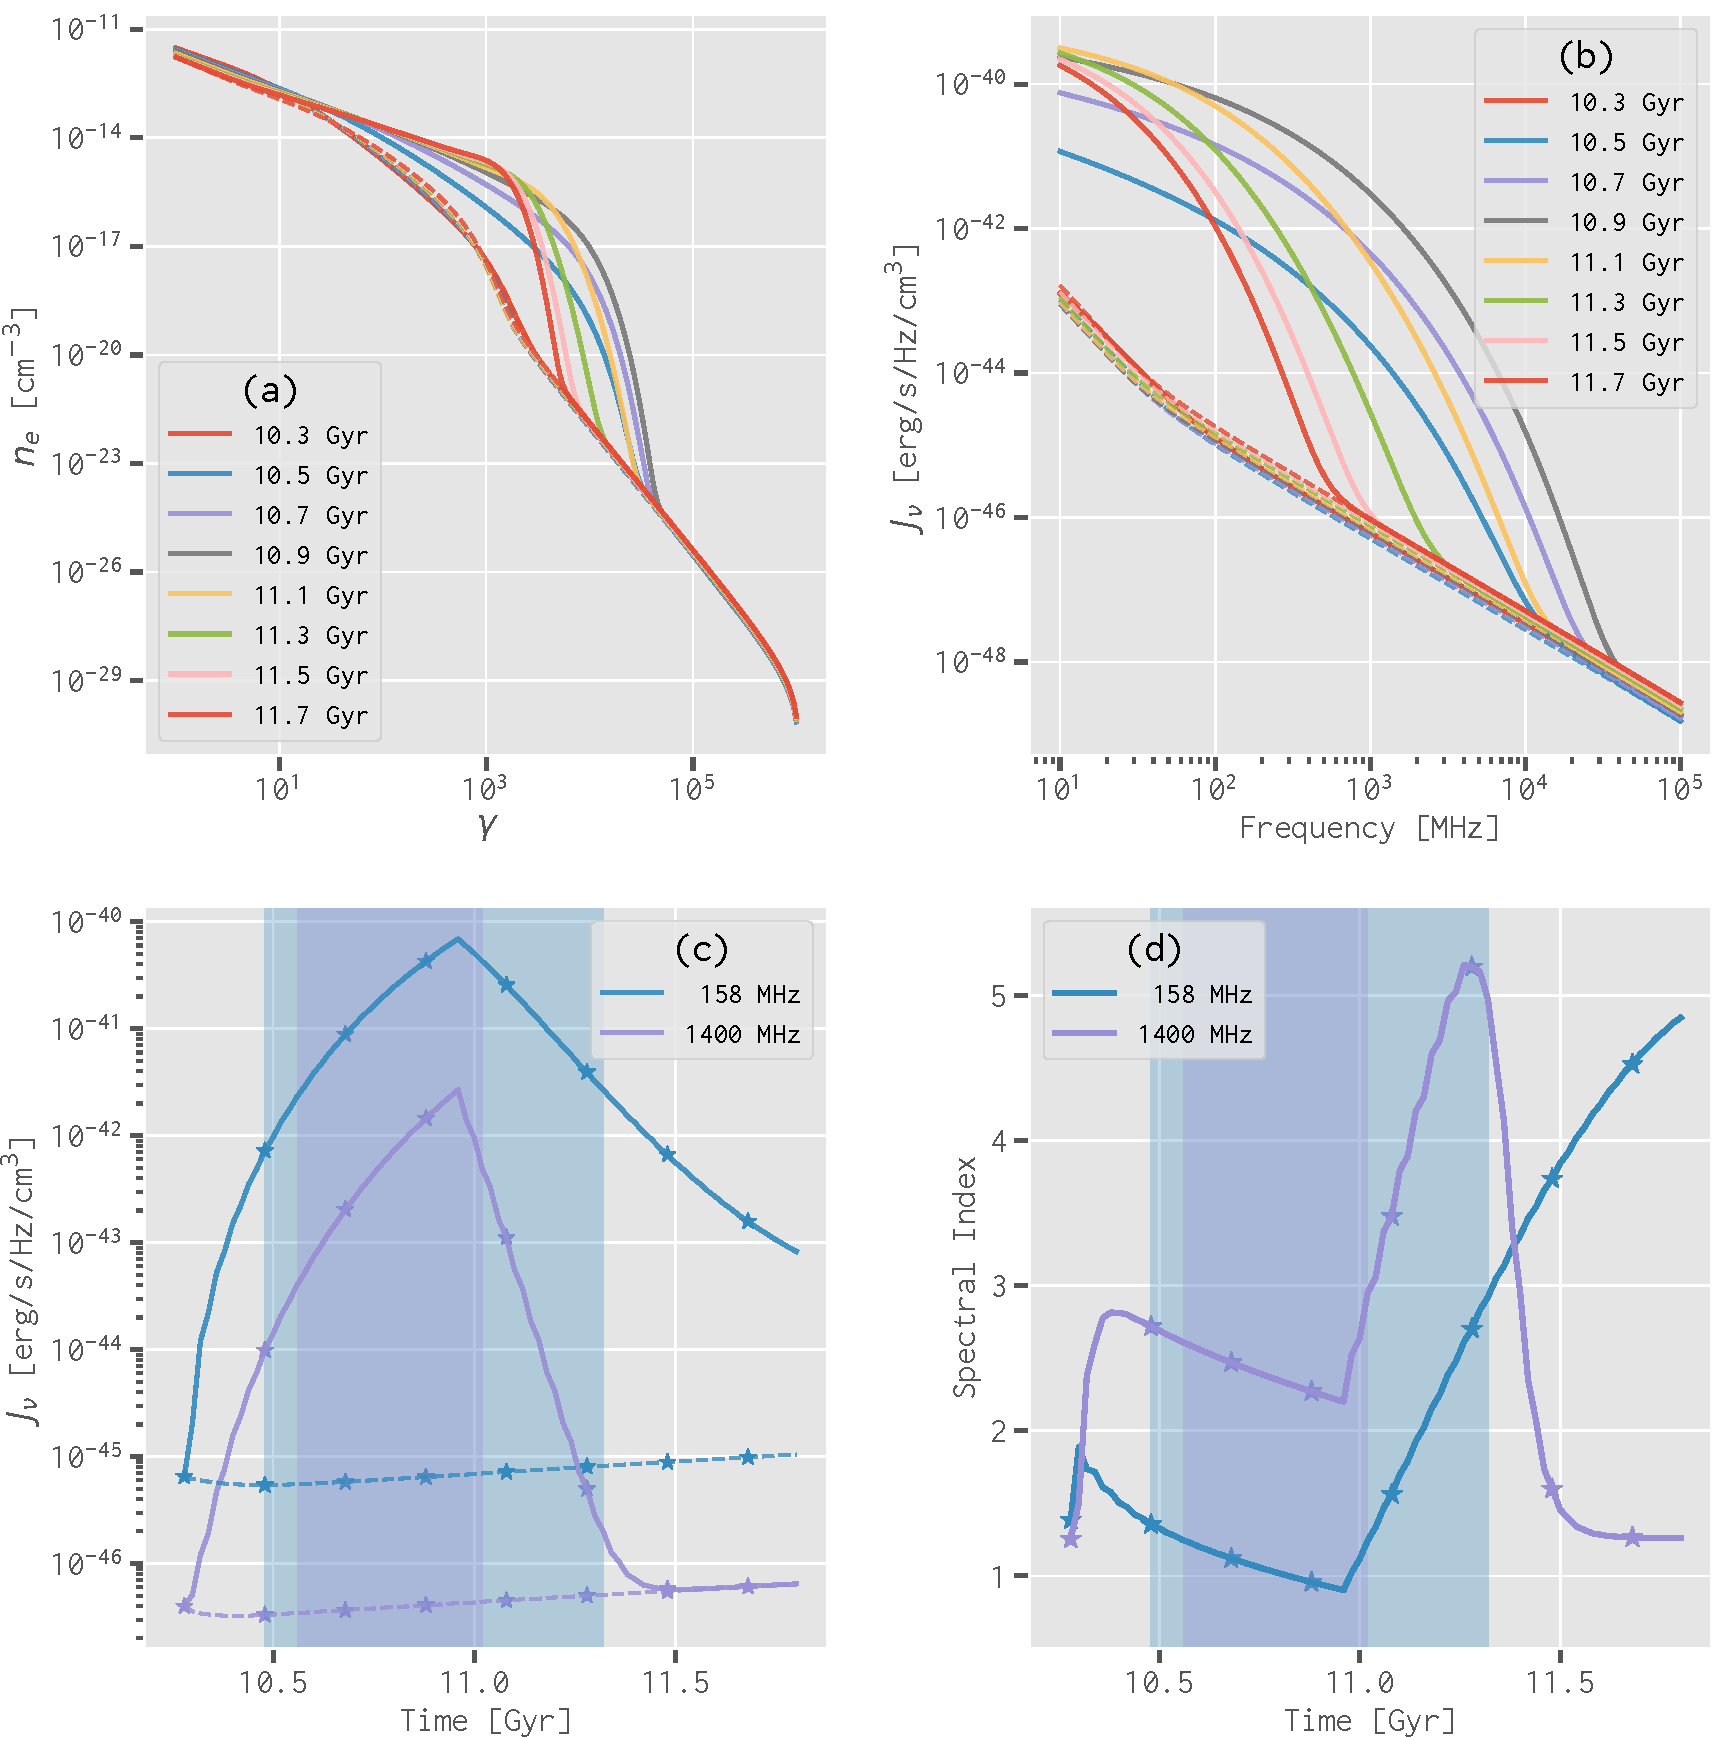
\includegraphics[width=0.95\textwidth]{spec-evo-example}
  \bicaption[电子能谱和同步辐射频谱随时间的演化示例]{%
    一个在红移 $z = 0.3$ ($t \simeq \SI{10.3}{\Gyr}$)
    经历了一次\acs*{m-major}的星系团从并合开始至
    $z = 0.15$ ($t \simeq \SI{11.8}{\Gyr}$)
    的高能电子能谱 \acs*{n-e} 和\acl*{syn-em}频谱
    $\acs*{syn-em}(\nu)$ 随时间的演化.
    \textbf{(a)}
    高能电子能谱(实线)和相应的参考能谱(虚线;见 \autoref{sec:halo-size});
    \textbf{(b)}
    \acl*{syn-em}频谱(实线)和相应的参考频谱(虚线);
    \textbf{(c)}
    同步辐射在 \SI{158}{\MHz} (蓝色实线)和 \SI{1400}{\MHz} (紫色实线)
    处的发射率及其相应的参考发射率(虚线)随时间的变化;
    \textbf{(d)}
    \SI{158}{\MHz} (蓝线)和 \SI{1400}{\MHz} (紫线)处的谱指数随时间的变化.
    阴影区域显示了射电晕存在的时间段(详见 \autoref{sec:halo-size}).
    星号标记了显示在子图 (a) 和 (b) 中的频谱所对应的时间点.
  }{%
    The temporal evolution of the electron and synchrotron
    emissivity spectra for an example cluster with one major merger,
    which begins at redshift $z = 0.3$ (i.e., $t \simeq \SI{10.3}{\Gyr}$)
    and is tracked until $z = 0.15$ (i.e., $t \simeq \SI{11.8}{\Gyr}$).
    \textbf{(a)} The relativistic electron spectra (solid lines) and the
    corresponding reference electron spectra (dashed lines; see
    \autoref{sec:halo-size}).
    \textbf{(b)} The synchrotron emissivity spectra (solid lines) and the
    corresponding reference synchrotron spectra (dashed lines).
    \textbf{(c)} The variation of \SI{158}{\MHz} (solid blue line) and
    \SI{1400}{\MHz} (solid purple line) synchrotron emissivity as well as
    the corresponding reference emissivity (dashed lines) with time.
    \textbf{(d)} The temporal variation of spectral indices at
    \SI{158}{\MHz} (blue line) and \SI{1400}{\MHz} (purple line).
    Shaded regions show the periods during which the radio halo exists
    (see \autoref{sec:halo-size}).
    Asterisks mark the time points corresponding to the spectra presented
    in panels (a) and (b).
  }
  \label{fig:spec-evo}
\end{figure}

以一个经历一次\ac{m-major}、质量为 \SI{e15}{\solarmass} 的星系团为例,
\autoref{fig:spec-evo} 显示了并合过程中高能电子能谱 \ac{n-e}
和\acl{syn-em}频谱 $\ac{syn-em}(\nu)$ 随时间的演化.
星系团在红移 $z = 0.3$ (对应宇宙年龄 $t \simeq \SI{10.3}{\Gyr}$)
时与一个质量为 \SI{6e14}{\solarmass} 的子团开始并合.
该并合的有效加速时长约为 $\tau_{\R{turb}} \simeq \SI{0.67}{\Gyr}$,
使电子被加速到极高能量 ($\gamma \gtrsim \num{e4}$),
形成在中高频段 ($> \si{\GHz}$) 可见的\ac{rh}.
然而,当并合从 $t > \SI{10.9}{\Gyr}$ 起停止活动时,
高能端的电子迅速地损失能量而衰减,\ac{rh}也很快地消失,特别是在中高频段.

%---------------------------------------------------------------------
\subsection{识别和大小}
\label{sec:halo-size}

从上一节的示例可知,如果 \ac{icm} 中没有活跃的湍流加速,
\ac{rh}要么无法形成要么会迅速消失.
通过求解 Fokker--Planck 方程 [\autoref{eq:fokkerplanck}]
并得到对应\ac{gc}\enquote{当前}时刻的高能电子能谱 $n_e(\ac{g}, t_{\R{sim}})$ 后,
还需要判别\ac{rh}在频率 $\nu$ 处是否确实存在.
为此,本工作采用以下两点判据:
\begin{enumerate}
  \item \acl{syn-em}在频率 $\nu$ 的值 $\ac{syn-em}(\nu)$
    是相应的\enquote{参考值} $J'_{\R{syn}}(\nu)$ 的至少 1000 倍.
    该参考值 $J'_{\R{syn}}(\nu)$ 由相应的参考电子能谱
    $n'_e(\ac{g}, t_{\R{sim}})$ 确定,
    后者的计算方法与 \autoref{sec:numerical} 中计算初始电子能谱
    $n_e(\ac{g}, t_0)$ 的方法类似,
    即在没有并合引起的湍流加速的情况下求解 Fokker--Planck 方程而得到.

  \item 同步辐射在频率 $\nu$ 处谱指数满足 $\alpha_{\nu} \le 3$.
\end{enumerate}

对于\autoref{fig:spec-evo} 所示的例子,
\ac{rh} 在 \SI{1.4}{\GHz} 处的存在时间段约为 \SIrange{10.6}{11.0}{\Gyr},
在 \SI{158}{\MHz} 处的存在时间段约为 \SIrange{10.5}{11.3}{\Gyr}.
同时,\ac{rh}的同步辐射频谱在 \SI{1.4}{\GHz} 和 \SI{158}{\MHz}
的谱指数分别达到了约 2.1 和 1.0.
这些结果显示,\ac{rh}在低频波段 ($\lesssim \SI{200}{\MHz}$) 更容易形成,
并且拥有更长的寿命.
因此,在低频波段也更容易发现更多的\ac{rh}.
此外,上述示例给出的 \SI{1.4}{\GHz} 谱指数 ($\alpha_{1400} \sim 2.1$)
比通常的观测结果\cite{feretti2012}偏大一些,
这是因为本工作直接在一个频率 $\nu$ 附近计算该频率处的谱指数 $\alpha_{\nu}$,
而观测给出的谱指数 $\alpha_{\nu_1}^{\nu_2}$ 通常由两个相隔较远的频率
($\nu_1$ 和 $\nu_2$) 的观测数据得出,比如 0.3 和 1.4 GHz \cite{feretti2012}.

判别一个\ac{rh}存在后,接着需要确定其大小.
之前的研究已显示\acl{r-halo} \ac{r-halo}
会随\ac{gc}的\acl{r-vir} \ac{r-vir} 超线性地增大 \cite{cassano2007,basu2012},
这可能是由于高能电子和磁场的径向分布特征造成的 \cite{dolag2002}.
据此,本工作假定\acl{r-halo} \ac{r-halo} 满足以下\ac{scaling-relation}:
\begin{equation}
  \label{eq:r-halo}
  \ac{r-halo} = f_r \ac{R-turb}
    \left( \frac{\ac{r-vir}}{r_{\R{vir,*}}} \right)^b ,
\end{equation}
其中
\ac{R-turb} 是最大湍流区域的半径 [另见\autoref{eq:ratio-v}],
$r_{\R{vir,*}}$ 是质量为 \SI{e15}{\solarmass} 的参考星系团的\acl{r-vir},
$f_r$ 和 $b$ 分别是\ac{scaling-relation}的系数和指数.
\citeay{cassano2007} 获得的观测\ac{scaling-relation}为:
$\ac{r-halo} \propto r_{\R{vir}}^{2.63 \pm 0.50}$,
与之对比后,本工作选取 $f_r = 0.7$ 和 $b = 1.8$.

于是,\ac{rh}在频率 $\nu$ 处的功率 $\ac{P-halo}(\nu)$ 为:
\begin{equation}
  \label{eq:halo-power}
  \ac{P-halo}(\nu) = \frac{4\Cpi}{3} r_{\R{halo}}^3 \ac{syn-em}(\nu) ,
\end{equation}
同时在该频率处的流量密度 $\ac{S-halo}(\nu)$ 为:
\begin{equation}
  \label{eq:halo-flux}
  \ac{S-halo}(\nu) =
    \frac{(1+z_{\R{sim}}) \,\ac{P-halo}[\nu(1+z_{\R{sim}})]}{
      4\Cpi D_{\!L}^2(z_{\R{sim}})} ,
\end{equation}
其中
$\acs{D-luminosity}(z_{\R{sim}})$ 是\ac{rh}的\acl{D-luminosity},
因子 $(1 + z_{\R{sim}})$ 用于考虑 $K$ 修正 \cite{hogg1999}.

%---------------------------------------------------------------------
\subsection{模型参数和结果}
\label{sec:halo-results}

本工作对\ac{rh}构建的模型主要包含以下 5 个待调节的参数:
\begin{enumerate}
  \item \ac{f-injection}:
    注入电子的总能量密度与 \ac{icm} 热能密度 \ac{e-th} 之比;
  \item \ac{f-trans}:
    并合释放的能量中转化为湍流能量的比例;
  \item \ac{f-cr}:
    宇宙射线的能量密度与 \ac{icm} 热能密度 \ac{e-th} 之比;
  \item \ac{f-turb}:
    初始湍流的能量密度与 \ac{icm} 热能密度 \ac{e-th} 之比;
  \item \ac{f-instability}:
    \ac{icm} 等离子体的不稳定性参数.
\end{enumerate}
由于目前的观测和理论研究均无法给出上述参数的有效约束,
因此有必要仔细调节这些参数,使得模型给出的结果能够符合目前的观测结果,
主要包括\ac{fluxfunc}、射电晕的功率与宿主星系团的质量之间的\ac{scaling-relation}.

我们通过以下两个对比来调节上述参数.
第一个对比是射电晕的 \SI{1.4}{\GHz} 功率 ($P_{1400}$)
与宿主星系团的维里质量 (\ac{M-vir}) 之间的\ac{scaling-relation}.
观测的\ac{scaling-relation}由 \citeay{cassano2013} 给出:
$P_{1400} \propto M_{500}^{3.70 \pm 0.56}$.
这里需要将质量 $M_{500}$ 换算至维里质量以便与模拟结果对比,
具体换算方法可见附录 \autoref{sec:r-m-conv}.

另一个对比则利用 \SI{1.4}{\GHz} 全天积分的 \ac{fluxfunc}.
为此,我们搜集了目前(截至 2018 年 1 月;TODO)已观测到的 80 个\ac{rh},
其中 71 个已确认,另外 9 个为候选,
详见\autoref{app:halos} 中的\autoref{tab:halos}.
考虑到目前观测到的\ac{rh}远不完备,尤其是在低流量端,
因此在对比时只要求模拟得到的\ac{fluxfunc}与观测结果在高流量端一致.

\begin{figure}[htp]
  \centering
  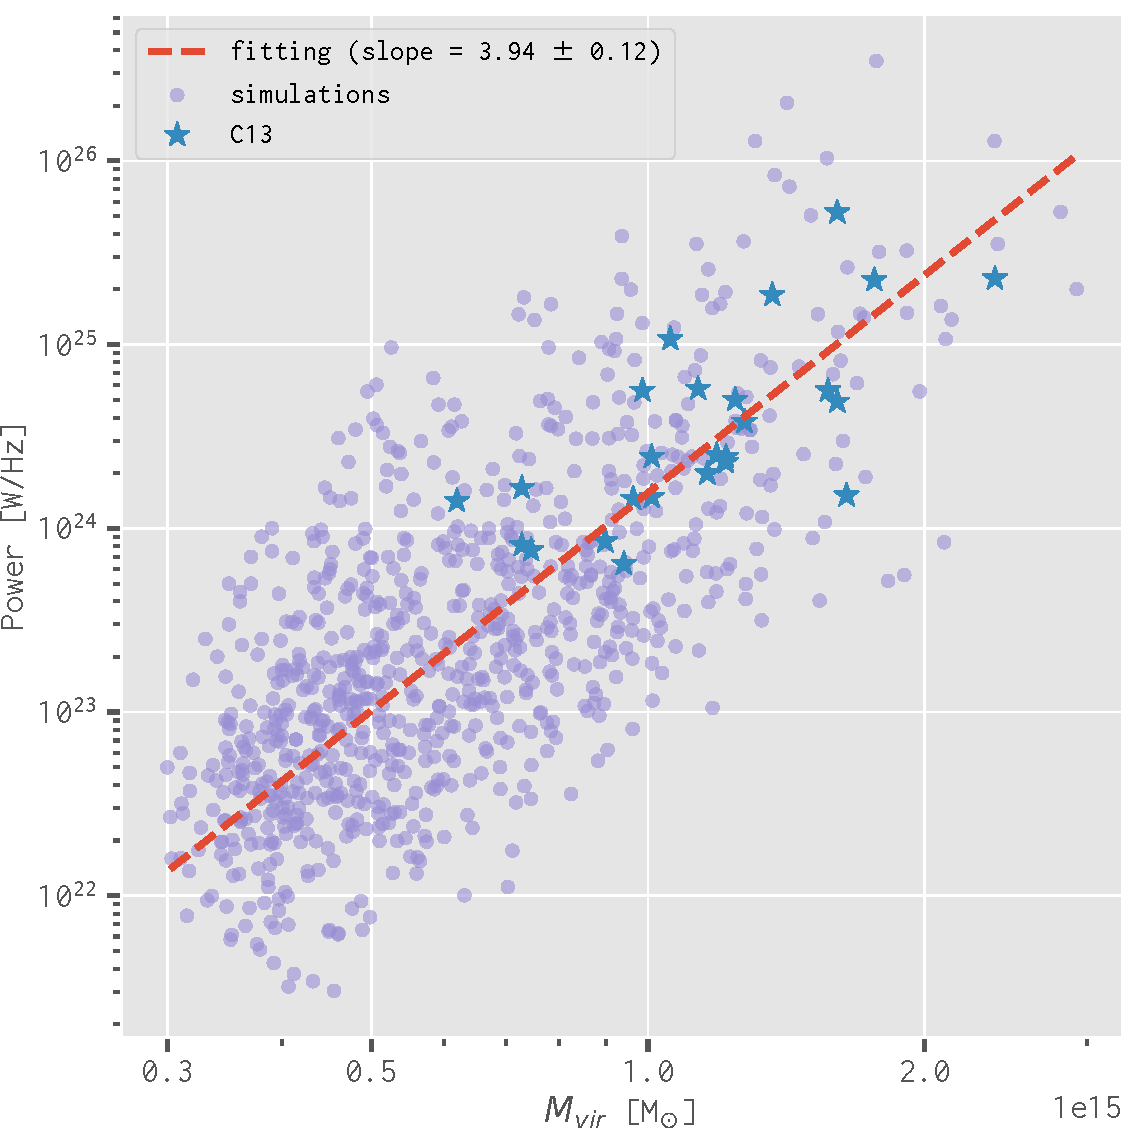
\includegraphics[width=0.7\textwidth]{halo-power-mvir}
  \bicaption[射电晕 \SI{1.4}{\GHz} 功率和宿主星系团质量之间的标度关系]{%
    模拟得到的射电晕 \SI{1.4}{\GHz} 功率 ($P_{1400}$) 和宿主星系团质量
    (\acs*{M-vir}) 之间的标度关系.
    蓝色星号表示来自 \citeay{cassano2013} 的观测数据.
    紫色圆点表示 500 次模拟的结果,红色虚线为模拟结果的拟合线:
    $P_{1400} \propto M_{\R{vir}}^{3.94 \pm 0.12}$.
  }{%
    Simulated scaling relation between the radio halo power at
    \SI{1.4}{\GHz} ($P_{1400}$) and the cluster mass (\acs*{M-vir}).
    Blue asterisks mark the observation data from \citeay{cassano2013}.
    Purple dots represent the results of 500 simulation runs
    and the dashed red line shows the fitted relation of
    $P_{1400} \propto M_{\R{vir}}^{3.94 \pm 0.12}$.
  }
  \label{fig:halo-power}
\end{figure}

\begin{figure}[htp]
  \centering
  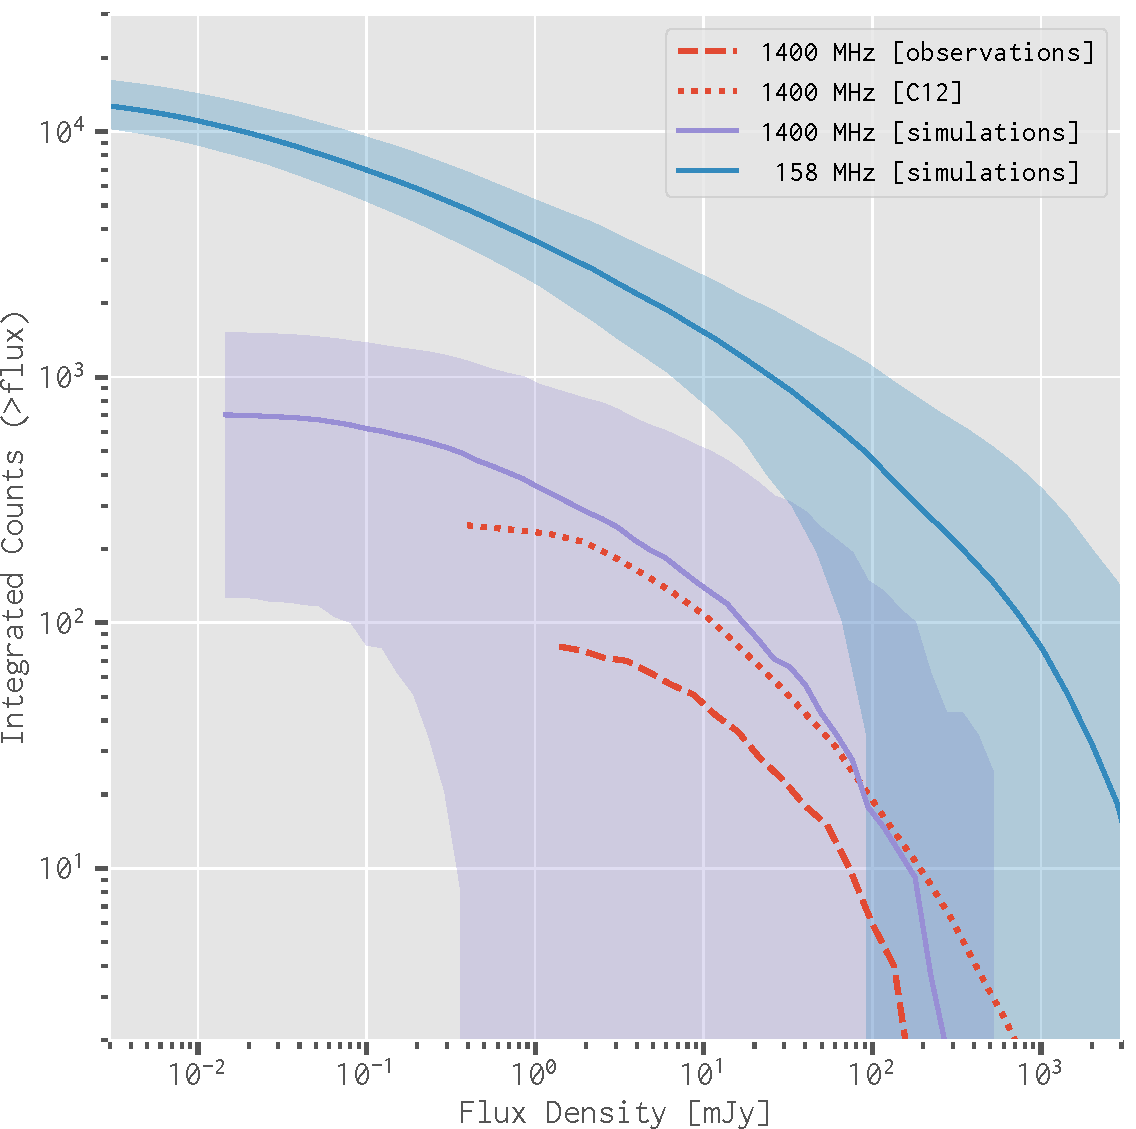
\includegraphics[width=\textwidth]{fluxfunc-simucomp}
  \bicaption[射电晕 \SI{1.4}{\GHz} 流量函数的对比]{%
    模拟的射电晕(紫色实线)和观测的射电晕(红色虚线)之间的
    \SI{1.4}{\GHz} 流量函数对比.
    红色点线显示了 \citeay{cassano2012} 预测的 \SI{1.4}{\GHz} 流量函数.
    作为对比,蓝色实线表示模拟的射电晕的 \SI{158}{\MHz} 流量函数.
    阴影区域显示了从 500 次模拟估算得到的 68\% 误差范围.
  }{%
    The \SI{1.4}{\GHz} all-sky integrated flux function comparison
    between the simulated (solid purple line) and observed
    (dashed red line) radio halos.
    The dotted red line shows the \SI{1.4}{\GHz} flux function
    predicted by \citeay{cassano2012}.
    The solid blue line represents the \SI{158}{\MHz} flux function for
    the simulated halos as a comparison.
    Shaded regions mark the 68\% uncertainties of the
    simulated radio halos estimated from the 500 simulation runs.
  }
  \label{fig:halos-simucomp}
\end{figure}

根据上述 $P_{1400}$--\ac{M-vir} \ac{scaling-relation}可知,
亮射电晕主要位于大质量 ($\gtrsim \SI{e15}{\solarmass}$) 星系团中.
在一片 \SI{10 x 10}{\degree} 的天区里,
大质量星系团有显著的涨落 (\autoref{sec:mass-function}),
因此亮射电晕也会出现明显的涨落.
为了考虑这个分布涨落,我们对每一种参数组合均重复模拟 500 次,
由此估算模拟结果的均值和误差,并与上述两点观测结果进行对比.
通过测试多种参数组合,最终选取如下一组参数:
$\ac{f-injection} = 0.01\%$、
$\ac{f-trans} = 15\%$、
$\ac{f-cr} = 1.5\%$、
$\ac{f-turb} = 1.5\%$ 以及
$\ac{f-instability} = 0.1$.

如\autoref{fig:halo-power} 所示,使用上述调节好的参数,
模拟的射电晕给出的 $P_{1400}$--\ac{M-vir} \ac{scaling-relation}为:
$P_{1400} \propto M_{\R{vir}}^{3.94 \pm 0.12}$.
该\ac{scaling-relation}的斜率和截距与 \citeay{cassano2013}
获得的观测结果都符合得很好.
\autoref{fig:halos-simucomp} 显示了 \SI{1.4}{\GHz} \ac{fluxfunc}
的对比结果,可见模拟的射电晕与观测的射电晕在高流量端是一致的.
同时,本工作模拟给出的 \SI{1.4}{\GHz} \ac{fluxfunc}
还与 \citeay{cassano2012} 的预测结果是匹配的.

此外,\autoref{fig:halo-fraction} 显示了具有射电晕的星系团比例
随星系团质量的变化.
显然,星系团的质量越大,其中存在射电晕的概率就越高.
同时,星系团中存在一个在低频波段(如 \SI{158}{\MHz})可见的射电晕的概率
也显著高于存在一个在高频波段(如 \SI{1.4}{\GHz})可见的射电晕.
因此,在低频波段 ($\sim \SIrange{100}{200}{\MHz}$) 将能观测到
成千上万个射电晕,远远多于目前发现的数目 \cite{cassano2012,cassano2015}.

\begin{figure}[htp]
  \centering
  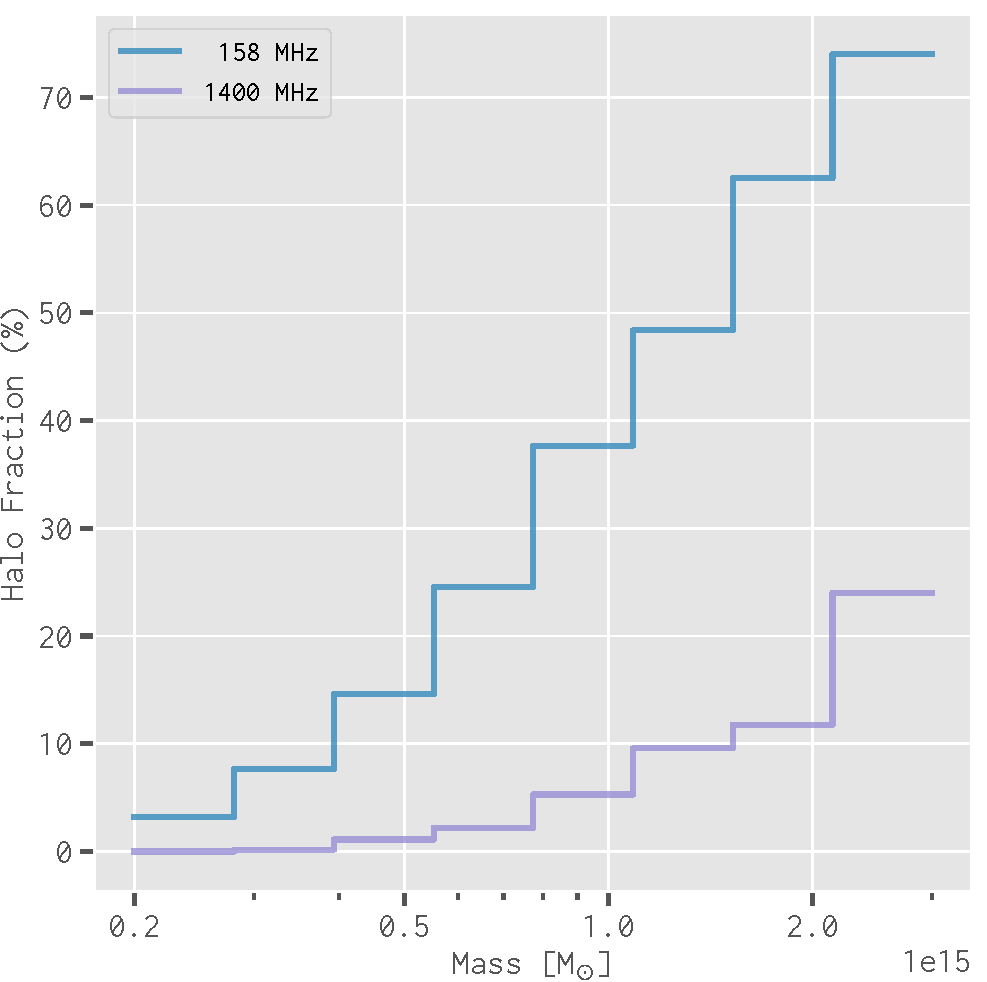
\includegraphics[width=0.7\textwidth]{halo-fraction}
  \bicaption[具有射电晕的星系团比例随星系团质量的变化]{%
    具有射电晕的星系团比例随星系团质量的变化.
    蓝线和紫线分别表示在 \SI{158}{\MHz} 和 \SI{1.4}{\GHz}
    频率处识别的射电晕比例.
  }{%
    The fraction of clusters with radio halos as a function of the cluster
    mass.
    The blue and purple lines represent the fraction of halos identified at
    \SI{158}{\MHz} and \SI{1.4}{\GHz}, respectively.
  }
  \label{fig:halo-fraction}
\end{figure}

%---------------------------------------------------------------------
\subsection{图像生成}
\label{sec:halo-maps}

获得射电晕的半径 \ac{r-halo} [\autoref{eq:r-halo}]
和流量密度 $\ac{S-halo}(\nu)$ [\autoref{eq:halo-flux}] 后,
为了生成图像,我们假定射电晕是圆形的,
并采用以下指数型轮廓来描述其角向平均的亮度分布 \cite{murgia2009}:
\begin{equation}
  \label{eq:halo-profile}
  \ac{I-nu}(\theta) =
    I_{\nu,0} \exp\left( -\frac{3\,\theta}{\theta_{\R{halo}}} \right) ,
\end{equation}
其中
$\theta = r / \acs{D-angular}(z_{\R{sim}})$ 是距离射电晕中心的角半径
(angular radius),
并且 $\ac{D-angular}(z_{\R{sim}})$ 是射电晕的\acl{D-angular};
$\theta_{\R{halo}} = \ac{r-halo} / \acs{D-angular}(z_{\R{sim}})$.
$I_{\nu,0}$ 为中心亮度,由射电晕的流量密度 $\ac{S-halo}(\nu)$ 确定:
\begin{align}
  \ac{S-halo}(\nu)
    & = \int_0^{\theta_{\R{halo}}} \ac{I-nu}(\theta) \,\D{\theta} \\
    & = I_{\nu,0} \int_0^{\theta_{\R{halo}}}
        \exp( -3\,\theta / \theta_{\R{halo}} ) \,\D{\theta} ,
\end{align}
于是可得:
\begin{equation}
  I_{\nu,0} = \frac{9 \ac{S-halo}(\nu)}{2\Cpi \theta^2_{\R{halo}}} .
\end{equation}
最后利用 Rayleigh--Jeans 近似 [\autoref{eq:rj-approx}],
便可以得到\ac{rh}的亮温度 $\acs{T-b}(\nu)$ 的分布图像.

如 \autoref{sec:halo-results} 所述,
为了考虑亮射电晕数目的显著涨落,使得\autoref{chap:halo}的评估结果更具代表性,
我们针对射电的模拟重复了 100 次,并将全部 100 次的模拟数据用于后续分析.
基于这 100 次模拟,射电晕的亮温度的\ac{rms}值的中位数以及 68\% 的误差\footnote{%
  68\% 的误差根据第 16 和第 84 百分位点 (percentile) 得到.
  对于弥散很大的数据,如此计算的误差比标准差更稳健 (robust).
}为:
在 \SI{124}{\MHz} 处是
$\left(4.21_{-2.60}^{+11.2}\right) \times 10^3$ \si{\mK};
在 \SI{158}{\MHz} 处是
$\left(1.81_{-1.13}^{+5.28}\right) \times 10^3$ \si{\mK};
以及在 \SI{196}{\MHz} 处是
$\left(0.85_{-0.54}^{+2.74}\right) \times 10^3$ \si{\mK}
(另见\autoref{tab:tb-rms}).
\autoref{fig:halos-skymap} 显示了其中一次典型情况的
射电晕在 \SI{158}{\MHz} 的模拟天图.

\begin{figure}[htp]
  \centering
  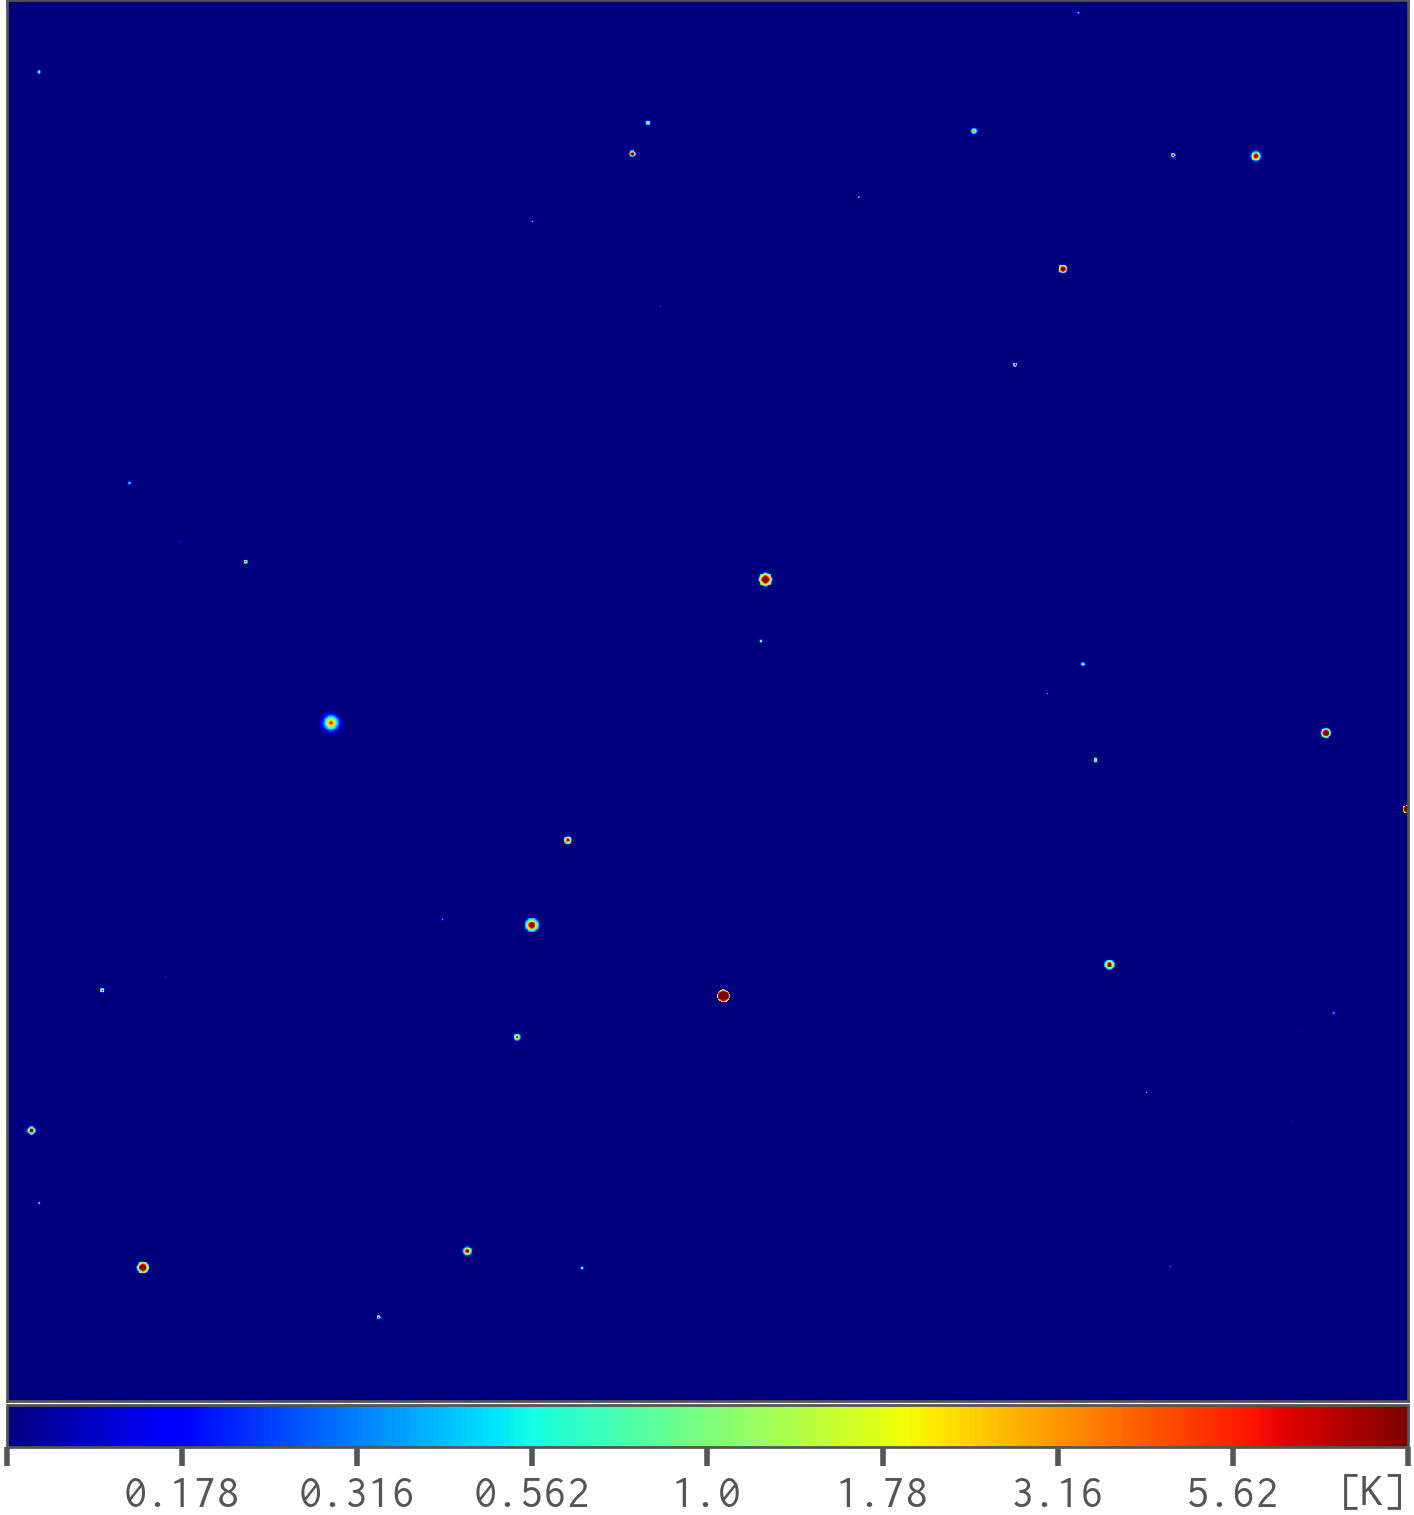
\includegraphics[width=0.8\textwidth]{skymap-halos-f158}
  \bicaption[射电晕在 \SI{158}{\MHz} 的模拟天图示例]{%
    射电晕在 \SI{158}{\MHz} 的模拟天图示例,为 100 次模拟中的一次典型情况.
    天区的大小为 \SI{10 x 10}{\degree},
    \ac{colorbar}以 \si{\kelvin} 为单位.
  }{%
    An typical example from the 100 simulation runs showing the
    simulated radio halos at \SI{158}{\MHz}.
    The sky region size is \SI{10 x 10}{\degree},
    and the color bar is in units of \si{\kelvin}.
  }
  \label{fig:halos-skymap}
\end{figure}

\begin{table}[htp]
  \centering
  \bicaption[所有成分的亮温度的\acs*{rms}值]{%
    所有成分的亮温度的\acs*{rms}值(单位: mK)
  }{%
    The Root-Mean-Square Brightness Temperatures of All Components
    (unit: mK)
  }
  \label{tab:tb-rms}

  \begin{tabular}{cccc}
    \toprule
    成分 & \SI{124}{\MHz} & \SI{158}{\MHz} & \SI{196}{\MHz} \\
    \midrule
    射电晕(100 次模拟) &
      $\left(4.21_{-2.60}^{+11.2}\right) \times 10^3$ &
      $\left(1.81_{-1.13}^{+5.28}\right) \times 10^3$ &
      $\left(0.85_{-0.54}^{+2.74}\right) \times 10^3$ \\
    银河系同步辐射 & \num{4.74e5} & \num{2.52e5} & \num{1.43e5} \\
    银河系自由--自由辐射 & \num{330} & \num{200} & \num{130} \\
    河外点源 & \num{29.7e7} & \num{5.90e7} & \num{1.39e7} \\
    EoR 信号 & \num{15.1} & \num{11.3} & \num{3.77} \\
    \bottomrule
  \end{tabular}
\end{table}


%=====================================================================
\section{银河系}

在低频波段,银河系的弥散辐射主要包括\ac{rad-syn}和\ac{rad-ff}.
本节将介绍如何模拟这两种辐射成分的图像.

银河系的辐射随天空位置而发生显著变化,越靠近银盘辐射越强,
因此 EoR 实验将挑选高银纬天区开展观测.
考虑到 SKA1-Low 将建设在 \ac{mwa} (\ang{26;42;12}\,S, \ang{116;40;16}\,E)
的旁边,同时 \ac{mwa} 目前正在研究的一块 EoR 天区位于
(R.A., Dec.\@) = (\SI{0}{\degree}, \SI{-27}{\degree}) \cite{beardsley2016},
该天区位于高银纬 ($b = \SI{-78.5}{\degree}$) 区域,
而且几乎经过望远镜的\ac{zenith},是一个理想的观测天区.
这个天区对本工作所开展的模拟研究而言是一个合适的选择(另见 \autoref{sec:obs-simu}).
因此,我们将以 (R.A., Dec.\@) = (\SI{0}{\degree}, \SI{-27}{\degree})
为中心坐标模拟银河系弥散辐射的天图.

%---------------------------------------------------------------------
\subsection{同步辐射}

TODO... simulation details...

The Galactic synchrotron map is simulated by extrapolating the
Haslam \SI{408}{\MHz} all-sky map as the template to lower frequencies
with a power-law spectrum.
We make use of the high-resolution version ($N_{\R{side}} = 2048$,
pixel size \SI{\sim 1.72}{\arcminute}) of the Haslam \SI{408}{\MHz}
map\footnote{The reprocessed Haslam \SI{408}{\MHz} map:
  \url{http://www.jb.man.ac.uk/research/cosmos/haslam_map/}},
which was reprocessed by \citeay{remazeilles2015} using significantly
better instrument calibration and more accurate subtraction of
extragalactic sources.
We also use the all-sky synchrotron spectral index map made by
\citeay{giardino2002} to account for the index variation with sky positions.
\autoref{fig:galactic-skymaps} 左栏显示了银河系\ac{rad-syn}在 \SI{158}{\MHz} 的天图.

\begin{figure}[htp]
  \centering
  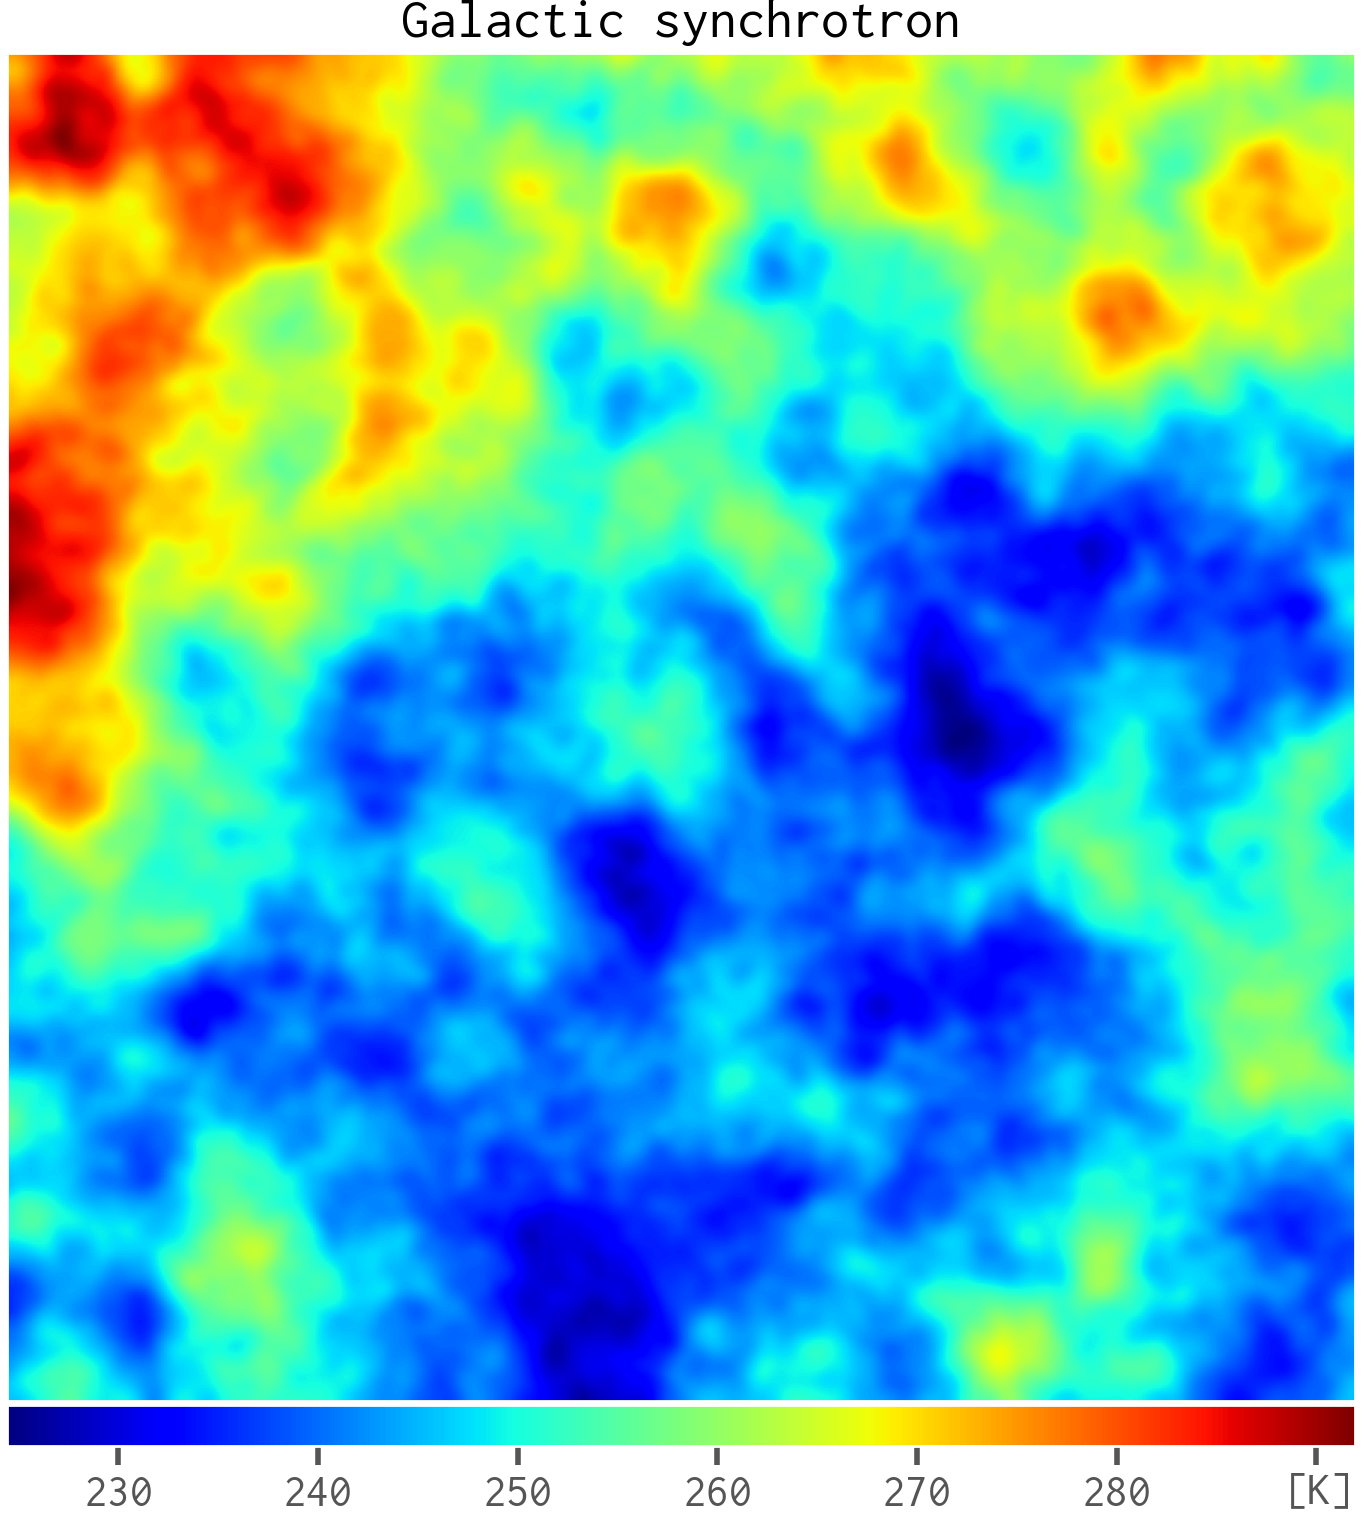
\includegraphics[width=0.498\textwidth]{skymap-gsyn-f158}%
  \hfill
  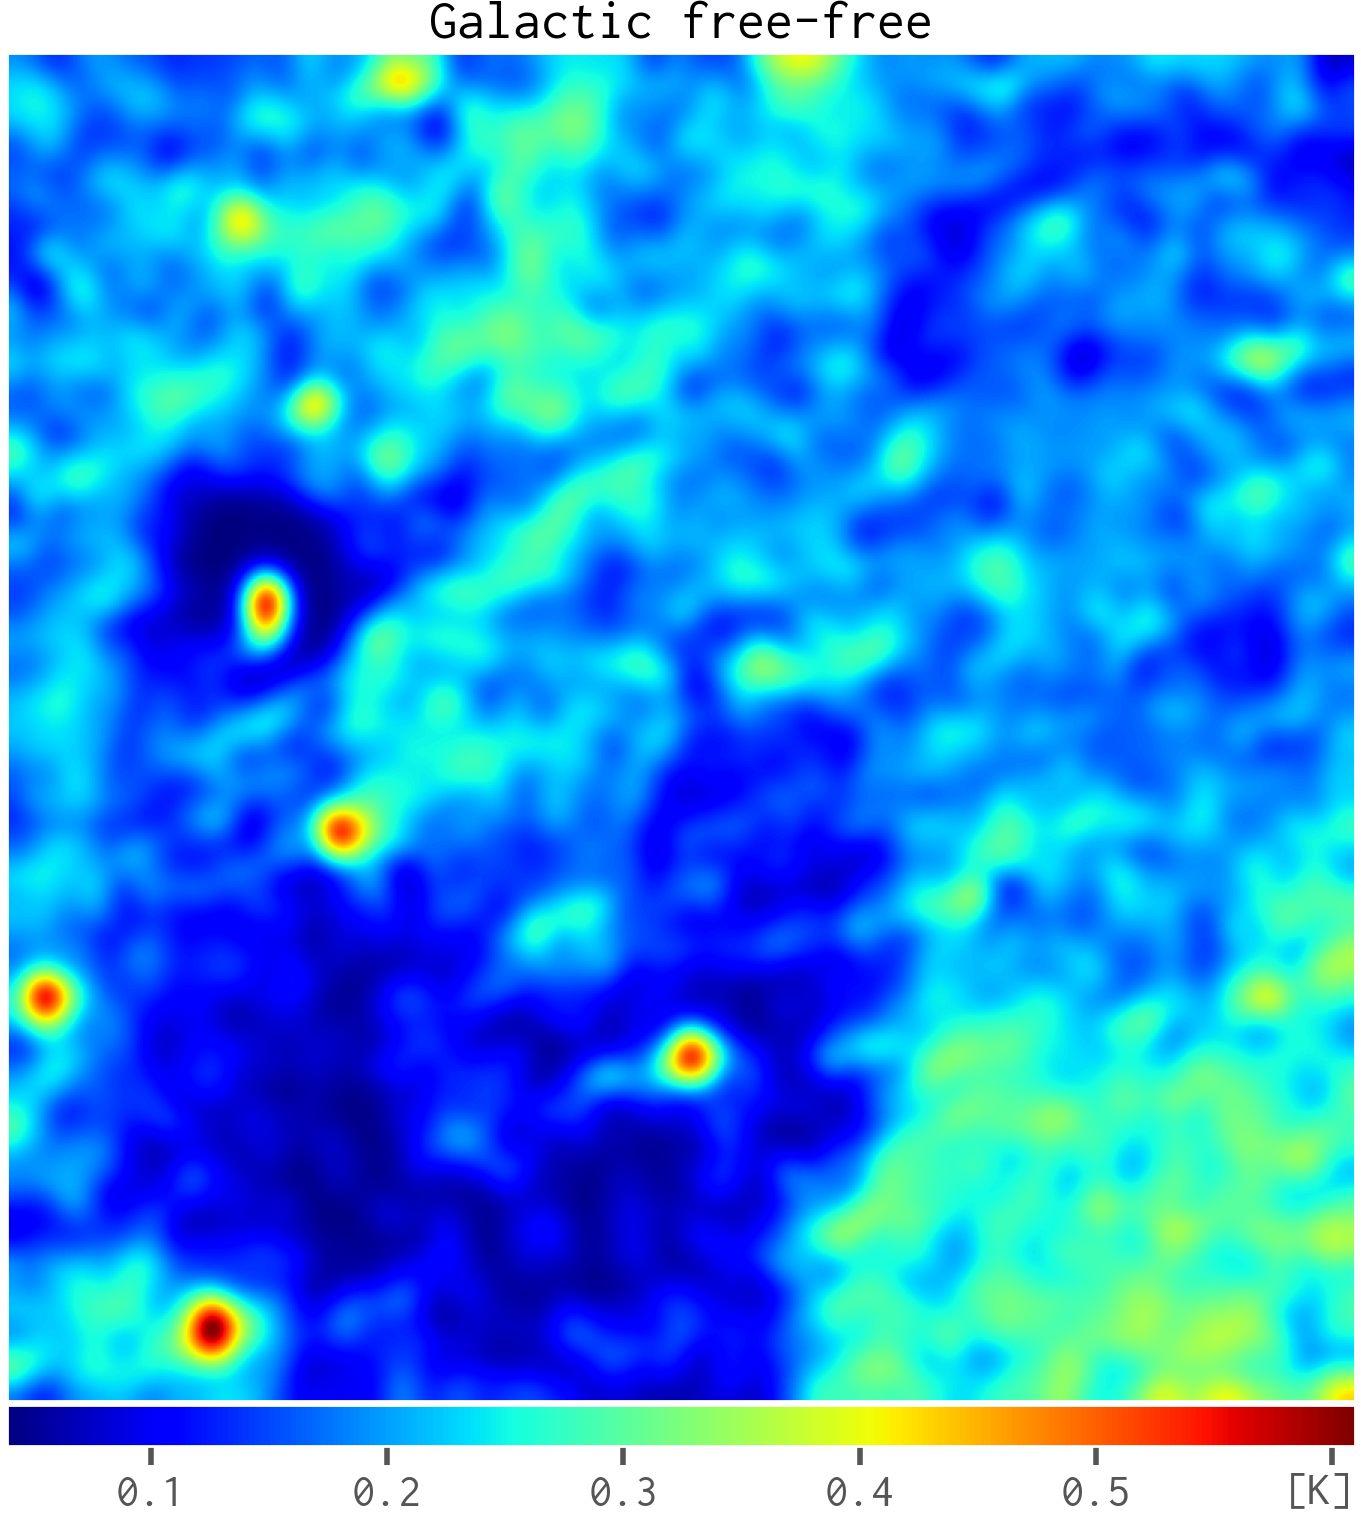
\includegraphics[width=0.498\textwidth]{skymap-gff-f158}
  \bicaption[银河系同步辐射和自由--自由辐射在 \SI{158}{\MHz} 的天图]{%
    TODO...
  }{%
    The sky maps of the Galactic synchrotron (left panel)
    and free-free (right panel) radiations at \SI{158}{\MHz}.
    Both maps have a sky region size of \SI{10 x 10}{\degree}
    and the color bars are in units of \si{\K}.
  }
  \label{fig:galactic-skymaps}
\end{figure}

%---------------------------------------------------------------------
\subsection{自由--自由辐射}
\label{sec:simu-gff}

TODO... simulation details...

The Galactic free-free emission is deduced from the Hα survey
data \cite{finkbeiner2003}, which is corrected for dust absorption,
by employing the tight relation between the Hα and free-free
emissions due to their common origins
(参考 \citeay{dickinson2003} 及其所引文献).
Since the Galactic diffuse emissions vary remarkably across the sky,
we simulate them at position of
(R.A., Dec.\@) = (\SI{0}{\degree}, \SI{-27}{\degree}), which locates at a
high galactic latitude ($b = \SI{-78.5}{\degree}$) and is expected to be
an appropriate choice for this study (see also \autoref{sec:obs-simu}).
\autoref{fig:galactic-skymaps} 右栏显示了银河系\ac{rad-ff}在 \SI{158}{\MHz} 的天图.


%=====================================================================
\section{河外点源}

TODO... simulation details

河外点源可大致分为以下几类 \cite{snellen2000,wilman2008,wang2010}:
(1) 恒星形成星系 (star-forming galaxy),
包括普通晚型星系 (normal late-type galaxy) 和星暴星系 (starburst galaxy);
(2) 射电宁静 (radio-quiet) \ac{agn};
(3) \ac{fr} I 型和 II 型 \ac{agn};
(4) GHz 倒转谱 (GHz-peaked-spectrum) \ac{agn};
(5) 致密陡谱 (compact steep-spectrum) \ac{agn}.

We simulate the former three types of sources by leveraging the simulation
results made by \citeay{wilman2008}, and simulate the latter two types
by employing their corresponding luminosity functions and spectral models.
More details can be found in \citeay{wang2010} and references therein.
\autoref{fig:ptrsrc-skymap} 显示了模拟的河外点源在 \SI{158}{\MHz} 的天图.

\begin{figure}[htp]
  \centering
  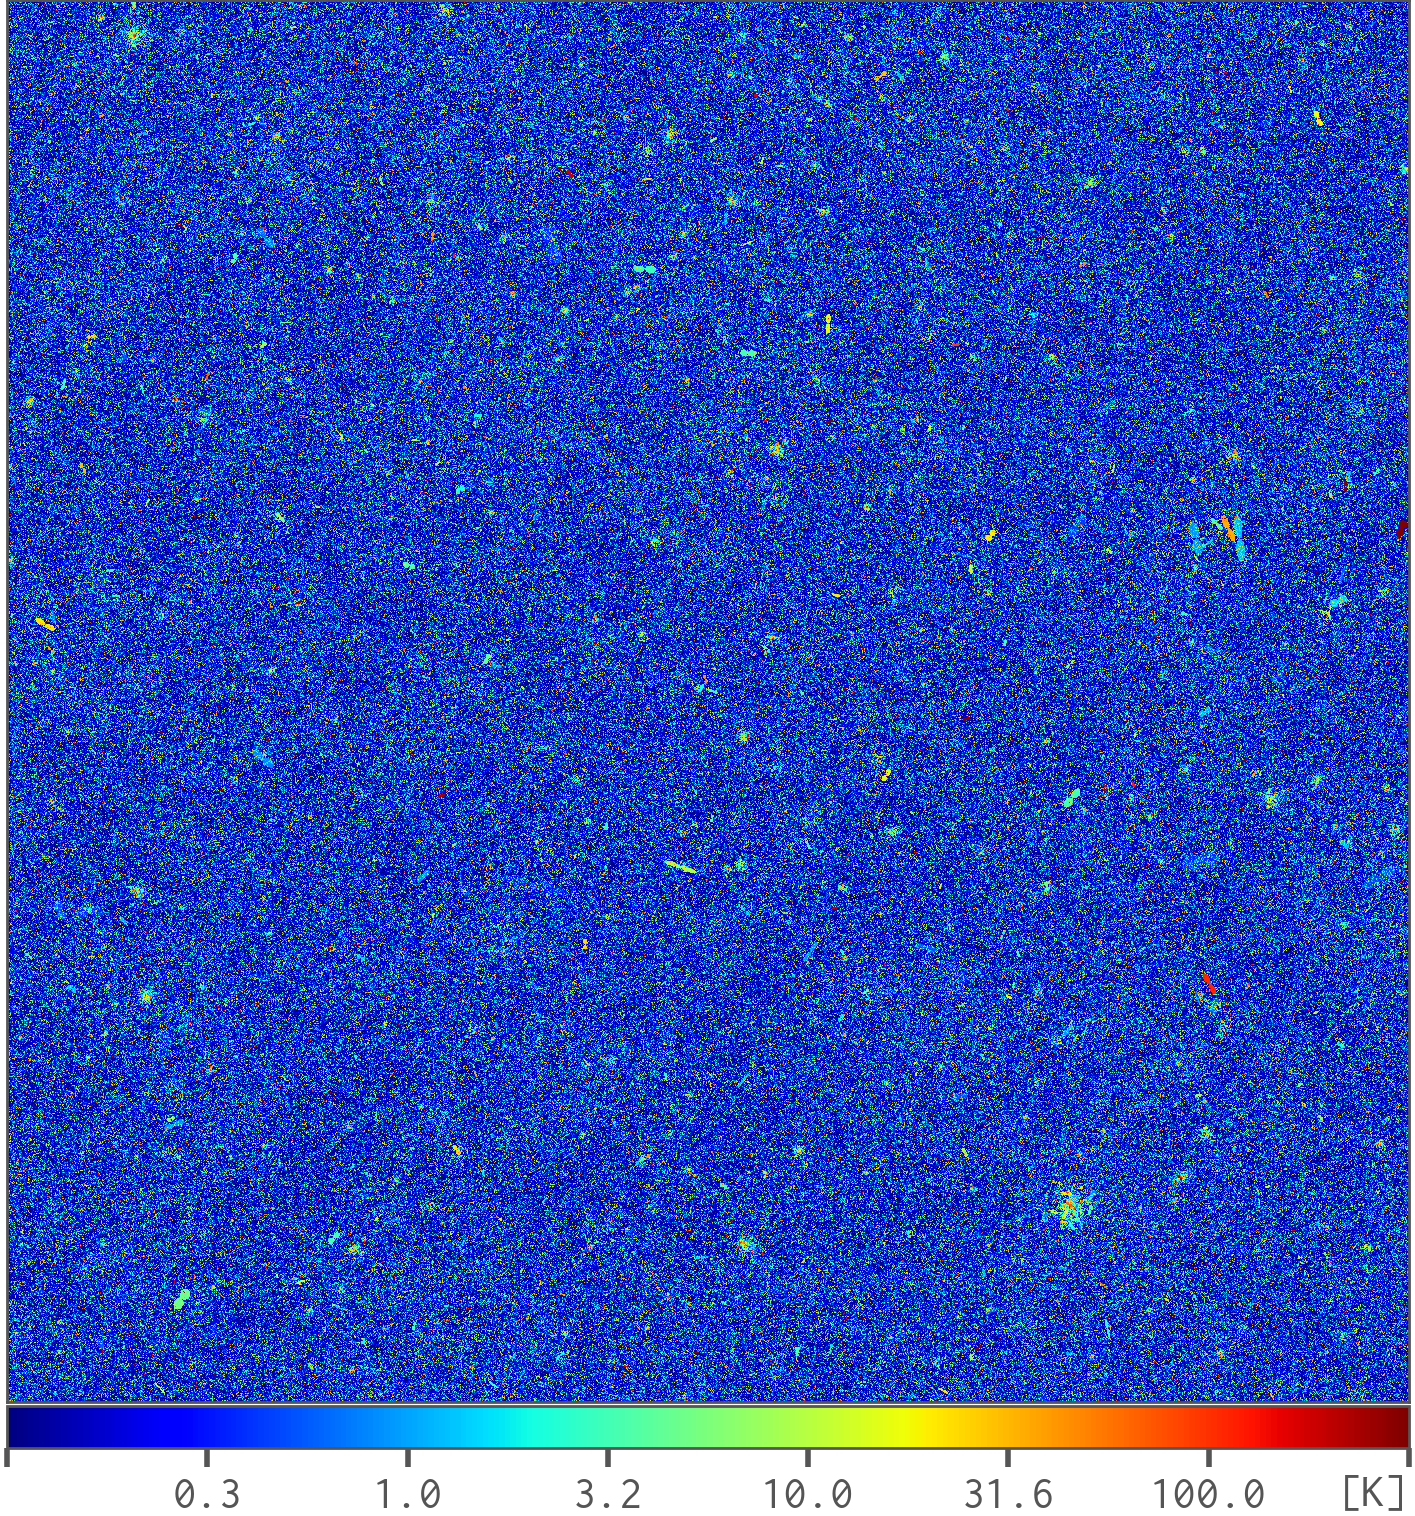
\includegraphics[width=0.7\textwidth]{skymap-ptrsrc-f158}
  \bicaption[河外点源在 \SI{158}{\MHz} 的模拟天图]{%
    TODO...
  }{%
    The simulated sky map of the extragalactic point sources at \SI{158}{\MHz}.
    The sky region size is \SI{10 x 10}{\degree}
    and the color bar is in units of \si{\K}.
  }
  \label{fig:ptrsrc-skymap}
\end{figure}


%=====================================================================
\section{EoR 信号}

The sky maps of the EoR signal are created using the 2016 data release
from the
\href{http://homepage.sns.it/mesinger/EOS.html}{Evolution Of 21\,cm Structure}
project\footnote{%
  Evolution Of 21\,cm Structure:
  \url{http://homepage.sns.it/mesinger/EOS.html}},
which has made use of the
\href{http://homepage.sns.it/mesinger/DexM___21cmFAST.html}{\texttt{21cmFAST}}%
\footnote{%
  21cmFAST: \url{http://homepage.sns.it/mesinger/DexM___21cmFAST.html}
} to simulate the cosmic
reionization process from redshift 86.5 to 5.0 inside a large cube that is
1.6 comoving \si{\Gpc} (1024 cells) along each side \cite{mesinger2016}.
We extract the image slices at needed frequencies (i.e., redshifts) from
the light-cone cubes of the recommended \enquote{faint galaxies} case,
and then tile and re-scale them to have the same sky coverage and
pixel size as our foreground maps.
\autoref{fig:eor-tbrms} shows the root-mean-square brightness temperatures of the
EoR signal among \SIrange{120}{200}{\MHz} ($z = \numrange{6.1}{10.8}$).
The corresponding root-mean-square brightness temperatures at the central
frequencies of the three adopted bands are given in \autoref{tab:tb-rms}
and the sky map of the EoR signal at \SI{158}{\MHz} is shown in
\autoref{fig:eor-skymap}.

\begin{figure}[htp]
  \centering
  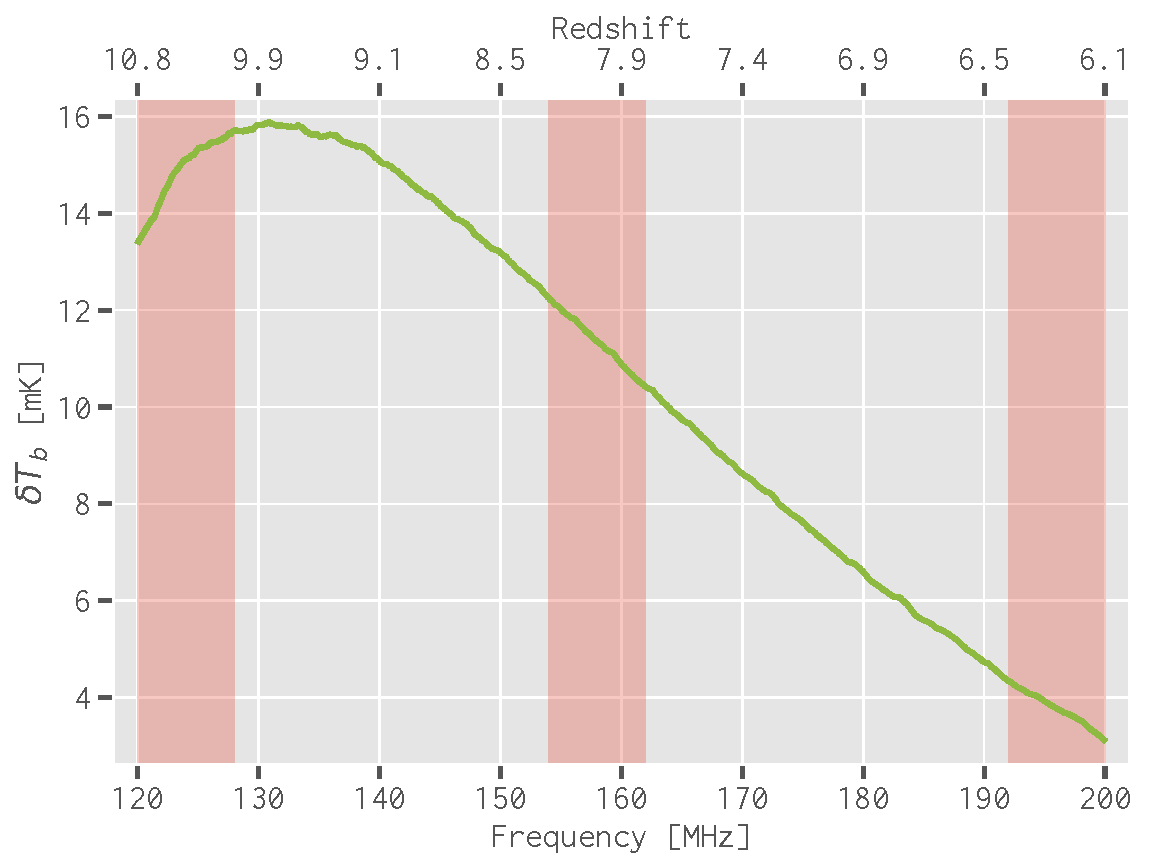
\includegraphics[width=0.8\textwidth]{eos2016-tbrms}
  \bicaption[EoR 信号在 \SIrange{120}{200}{\MHz} 的亮温度的\acs*{rms}值]{%
    TODO...
  }{%
    The root-mean-square brightness temperatures of the EoR signal
    (solid green line) within \SIrange{120}{200}{\MHz}
    ($z = \numrange{6.1}{10.8}$).
    The red shaded regions mark the three adopted frequency bands
    (\numrange{120}{128}, \numrange{154}{162}, and \numrange{192}{200}
    \si{\MHz}).
  }
  \label{fig:eor-tbrms}
\end{figure}

\begin{figure}[htp]
  \centering
  \includegraphics[width=0.7\textwidth]{skymap-eor-f158}
  \bicaption[EoR 信号在 \SI{158}{\MHz} 的天图]{%
    TODO...
  }{%
    The sky map of the EoR signal at \SI{158}{\MHz}.
    The sky region size is \SI{10 x 10}{\degree}
    and the color bar is in units of \si{\mK}.
  }
  \label{fig:eor-skymap}
\end{figure}


%=====================================================================
\section{干涉阵列的模拟观测}
\label{sec:obs-simu}

In order to properly evaluate the contamination of radio halos
on the EoR observations, it is essential to take account of the
practical instrumental effects of radio interferometers.

%---------------------------------------------------------------------
\subsection{SKA1-Low~阵列布局}

TODO: layout configuration, design goals, descriptions, figures...

Therefore, we employ the latest SKA1-Low layout configuration%
\footnote{\raggedright%
  SKA1-Low Configuration Coordinates:
  \url{https://astronomers.skatelescope.org/wp-content/uploads/2016/09/SKA-TEL-SKO-0000422_02_SKA1_LowConfigurationCoordinates-1.pdf}
  (released on 2016 May 21)
}
to simulate the SKA observations of the above simulated sky maps.
According to this layout configuration,
the SKA1-Low interferometer consists of 512 stations, with 224 of them
randomly distributed within the \enquote{core} of \SI{1000}{\meter} in
diameter, while the remaining stations are grouped into \enquote{clusters}
and placed on 3 spiral arms extending up to a radius of
\SI{\sim 35}{\kilo\meter}.
Each station has 256 antennas randomly distributed with a minimum separation
of $d_{\R{min}} = \SI{1.5}{\meter}$ inside a circular region of
\SI{35}{\meter} in diameter \cite{mort2017}.

%---------------------------------------------------------------------
\subsection{模拟观测和成像}

The \SI{8}{\MHz} bandwidth of each frequency band is divided into 51
channels for a frequency resolution of \SI{160}{\kilo\hertz}.
For each component, we simulate the input sky maps at every frequency
channel, and then use the
\href{https://github.com/OxfordSKA/OSKAR}{\texttt{OSKAR}}\footnote{%
  OSKAR: \url{https://github.com/OxfordSKA/OSKAR} (version 2.7.0)}
simulator \cite{mort2010} to perform observations for \SI{6}{\hour}.
The input sky maps are centered at sky position of
(R.A., Dec.\@) = (\SI{0}{\degree}, \SI{-27}{\degree}),
which passes through the zenith of the SKA1-Low telescope and
is an ideal choice for the simulation of SKA observations.
The simulated visibility data are imaged through the
\href{https://sourceforge.net/p/wsclean}{\texttt{WSClean}}\footnote{%
  WSClean: \url{https://sourceforge.net/p/wsclean} (version 2.6)}
imager \cite{offringa2014} using Briggs' weighting with a
robustness of zero \cite{briggs1995},
and the created images are cropped to keep only the central regions
because the marginal regions suffer from the problem of insufficient
CLEAN.
As the telescope's field of view (FoV) is inversely proportional to
the observing frequency, we choose to keep the central
\SI{6 x 6}{\degree}, \SI{5 x 5}{\degree}, and \SI{4 x 4}{\degree}
regions in the \numrange{120}{128}, \numrange{154}{162}, and
\numrange{192}{200} \si{\MHz} frequency bands, respectively.

The Galactic synchrotron and free-free emissions are combined for the
simulated observations because they have similar diffuse features.
Similar to the real-time peeling of the brightest point sources in
practical data analysis pipelines
\cite{mitchell2008,intema2009,mort2017},
we assume that extragalactic point sources with a \SI{158}{\MHz} flux
density $S_{158} > \SI{50}{\mJy}$ are removed
\cite{liu2009ps,pindor2011}.
Thus, the root-mean-square brightness temperatures of point sources
are significantly reduced to be about
\num{22.5e4}, \num{9.81e4}, and \num{4.75e4} \si{\mK}
at 124, 158, and 196 \si{\MHz}, respectively.
In addition, we create the foreground image cubes in each frequency band
using the CLEAN algorithm with joined-channel deconvolution in order
to ensure the spectral smoothness \cite{offringa2017}, which is crucial
to extract the faint EoR signal in the presence of overwhelming
foreground contamination.
For the EoR signal, we directly use the dirty images because the CLEAN
algorithm is not well applicable to such faint and diffuse emissions.
Hence we obtain the SKA \enquote{observed} image cubes of the EoR signal,
radio halos, the Galactic diffuse emission (with synchrotron and
free-free emissions combined), and the extragalactic point sources
(with the brightest ones removed) in the \numrange{120}{128},
\numrange{154}{162}, and \numrange{192}{200} \si{\MHz} frequency bands.


%=====================================================================
\section{小结}

TODO


%% EOF

%%
%% Copyright (c) 2018-2019 Weitian LI <liweitianux@sjtu.edu.cn>
%% Creative Commons BY 4.0
%%

\chapter{射电晕对宇宙再电离探测的影响}
\label{chap:halo}

%=====================================================================
\section{评估方法}
\label{sec:eval-method}

利用\autoref{chap:simulation}模拟得到的射电晕、
EoR 信号以及其他前景成分的 SKA1-Low \enquote{观测}图像,
我们可以定量地评估射电晕对 EoR 探测产生的影响,
分别针对\ac{fg-rm}和\ac{fg-avd}两类前景处理方法 (\autoref{sec:fg-methods})
进行评估.
首先,我们计算一维\ac{ps} $\ac{psD}(k)$ 来对比射电晕和 EoR 信号在各个尺度 $k$ 的功率,
说明使用\ac{fg-rm}方法时将面临的射电晕的污染强度.
其次,我们计算二维\ac{ps} $\ac{psD}(\ac{k-perp}, \ac{k-los})$,
然后在 EoR 窗口 (\autoref{sec:eor-window}) 内比较射电晕和 EoR 信号的功率,
据此评估使用\ac{fg-avd}方法提取 EoR 信号时射电晕的污染程度.

\begin{figure}[htp]
  \centering
  \includegraphics[width=\textwidth]{ft-sidelobes}
  \bicaption[加窗前后的 Fourier 变换结果对比]{%
    直接进行 Fourier 变换(红色实线)与
    使用 Blackman--Nuttall \acs*{f-window}之后再 Fourier 变换(蓝色虚线)
    的结果对比.
    左栏显示了加窗前后的输入信号 $y = (x/158)^{-2}$,
    右栏显示了相应的 Fourier 变换结果.
  }{%
    A comparison of the Fourier transform results with and without
    applying the Blackman--Nuttall window function.
    The left panel shows the original input signal $y = (x/158)^{-2}$
    (solid red line) and the windowed signal (dashed blue line);
    the right panel shows the corresponding Fourier transform results.
  }
  \label{fig:ft-sidelobes}
\end{figure}

考虑一个有限宽的频带,信号(如前景辐射)将在频带的两端出现跃变,
这种边界效应会导致 Fourier 变换的结果具有显著的\ac{sidelobe}.
即使输入信号非常平滑,Fourier 变换后也会出现一系列幅度较大的高频 Fourier 成分,
如\autoref{fig:ft-sidelobes} 所示.
为了抑制边界效应所产生的\ac{sidelobe},可以先对信号加窗,然后再进行 Fourier 变换.
一个常用的选择是 Blackman--Nuttall \ac{f-window},
该\ac{f-window}具有良好的\ac{sidelobe}性质 \cite{nuttall1981}:
\begin{equation}
  \label{eq:bn-window}
  w[n] = a_0 - a_1 \cos\left(\frac{2\Cpi n}{N}\right)
    + a_2 \cos\left(\frac{4\Cpi n}{N}\right)
    - a_3 \cos\left(\frac{6\Cpi n}{N}\right) ,
\end{equation}
其中
$N$ 为采样点的数目(即窗的宽度),
其他系数分别为:
$a_0 = \num{0.3635819}$,
$a_1 = \num{0.4891775}$,
$a_2 = \num{0.1365995}$,
$a_3 = \num{0.0106411}$.
\autoref{fig:ft-sidelobes} 显示了使用 Blackman--Nuttall 
\ac{f-window}之后得到的 Fourier 变换结果,
可见高频 Fourier 成分的幅度被有效地抑制了.
因此,我们对\autoref{chap:simulation}模拟得到的\ac{imgcube}沿频率方向施加
Blackman--Nuttall \ac{f-window},
然后再进行 Fourier 变换以及计算\ac{ps} \cite{trott2015,chapman2016}.


%=====================================================================
\section{一维功率谱}
\label{sec:ps1d}

我们对上一章模拟得到的每一个成分在每一个频带里的\ac{imgcube}分别计算了
一维\ac{ps} $\ac{psD}(k)$.
对于射电晕,我们使用了全部 100 次模拟 (\autoref{sec:halo-maps}) 的结果
来估算其一维功率谱的中位数和 68\% 的误差范围.
具体而言,在一个频带里,射电晕的 100 次模拟会生成 100 个\ac{imgcube},
分别计算这 100 个\ac{imgcube}的一维功率谱,
然后从所得的 100 个一维功率谱计算每个尺度 $k$ 处的中位数和相应的 68\% 误差范围.

\begin{figure}[htp]
  \centering
  \includegraphics[width=\textwidth]{ps1d-3bands}
  \bicaption[各成分在三个频带内的一维功率谱 $\ac{psD}(k)$ 对比]{%
    EoR 信号(绿色实线)、射电晕(红色实线)、银河系弥散辐射(灰色虚线)以及
    河外点源(灰色点虚线)之间的一维功率谱 $\ac{psD}(k)$ 的对比.
    左栏、中栏、右栏分别表示 \numrange{120}{128}、\numrange{154}{162}
    和 \numrange{192}{200} \si{\MHz} 三个频带的结果.
    对于射电晕,红色实线及其阴影区域分别表示从 100 次模拟结果得到的
    中位数和 68\% 的误差范围.
  }{%
    Comparisons of the 1D dimensionless power spectra $\ac{psD}(k)$
    among the EoR signal (solid green line), radio halos (solid red line),
    Galactic diffuse emission (dashed gray line), and extragalactic point
    sources (dash-dotted gray line) in the
    \textbf{(a)} \SIrange{120}{128}{\MHz},
    \textbf{(b)} \SIrange{154}{162}{\MHz}, and
    \textbf{(c)} \SIrange{192}{200}{\MHz} frequency bands.
    The solid red lines and shaded regions represent the median values
    and the corresponding 68\% uncertainties of the power
    spectra for radio halos estimated from the 100 simulation runs.
  }
  \label{fig:ps1d-3bands}
\end{figure}

\autoref{fig:ps1d-3bands} 显示了各成分在三个频带内的
一维功率谱 $\ac{psD}(k)$ 的对比.
可见,在 $\SI{0.1}{\per\Mpc} < k < \SI{2}{\per\Mpc}$ 尺度范围内,
射电晕的典型功率(红色实线)在 \numrange{120}{128}、\numrange{154}{162} 和
\numrange{192}{200} \si{\MHz} 频带内分别是 EoR 信号的功率的
\num{e4}、\num{e3} 和 \num{e2.5} 倍.
考虑到射电晕的亮度和数目在不同天区里会发生显著变化,
因此在 68\% 的误差范围内(红色阴影区域),
射电晕的功率能够变化约 \numrange{10}{100} 倍.

对于另外两个前景成分,银河系前景在最大尺度 ($k \lesssim \SI{0.1}{\per\Mpc}$)
上是最强的污染源,但随着尺度的减小(对应于 $k$ 增大),其功率也迅速减小.
在 $\SI{0.5}{\per\Mpc} \lesssim k \lesssim \SI{1}{\per\Mpc}$
的中小尺度范围,
射电晕的典型功率比银河系前景的功率强约 \numrange{10}{100} 倍.
河外点源除了在最大尺度上弱于银河系前景,在其他尺度上均是最强的污染源.

以上这些结果清楚地说明射电晕是严重的 EoR 前景污染源,需要在前景扣除中被仔细处理.
此外,射电晕的形态还呈现一定程度的不规则结构,这显著增加了对其准确建模和扣除的难度.


%=====================================================================
\section{二维功率谱}
\label{sec:ps2d}

\begin{figure}[htp]
  \centering
  \includegraphics[width=\textwidth]{ps2d-band158}
  \bicaption[%
    各成分在 \SIrange{154}{162}{\MHz} 频段的二维功率谱
    $\acs*{psD}(\acs*{k-perp}, \acs*{k-los})$%
  ]{%
    各成分在 \SIrange{154}{162}{\MHz} 频段的二维功率谱
    $\ac{psD}(\ac{k-perp}, \ac{k-los})$,
    从左上至右下分别为:
    \textbf{(a)} EoR 信号;
    \textbf{(b)} 射电晕(100 次模拟的中位数);
    \textbf{(c)} 银河系弥散辐射;
    \textbf{(d)} 河外点源.
    所有子图共用了以 [\si{\mK\squared\Mpc\cubed}] 为单位的对数\ac{colorbar}.
    白色虚线显示了 EoR 窗口的边界.
  }{%
    The \SIrange{154}{162}{\MHz} 2D power spectra
    $\ac{psD}(\ac{k-perp}, \ac{k-los})$ of
    \textbf{(a)} the EoR signal,
    \textbf{(b)} radio halos (median of the 100 simulation runs),
    \textbf{(c)} Galactic diffuse emission,
    and
    \textbf{(d)} extragalactic point sources.
    All panels share the same logarithmic scale in units of
    [\si{\mK\squared\Mpc\cubed}].
    The dashed white lines mark the boundary between the EoR window
    (at the top left) and the contaminating wedge (at the bottom right).
  }
  \label{fig:ps2d}
\end{figure}

以 \SIrange{154}{162}{\MHz} 频带为例,
\autoref{fig:ps2d} 显示了 EoR 信号、射电晕、银河系弥散辐射以及河外点源的
二维功率谱 $\ac{psD}(\ac{k-perp}, \ac{k-los})$,
其中射电晕的二维功率谱对应于 100 次模拟结果的中位数.
从图中容易看出,EoR 信号的功率分散在大范围的 \ac{k-los} \ac{mode}里,
反映了 EoR 信号沿频率维度快速变化的特点;
频谱光滑的前景成分则集中在 \ac{k-los} 较小的区域
($\ac{k-los} \lesssim \SI{0.2}{\per\Mpc}$).
在空间维度 (\ac{k-perp}),射电晕的功率主要出现在
$\ac{k-perp} \lesssim \SI{1}{\per\Mpc}$ 的范围,
并且倾向于集中在 $\ac{k-perp} \sim \SI{0.5}{\per\Mpc}$ 的中等尺度上.
银河系弥散辐射的功率主导了 $\ac{k-perp} \lesssim \SI{0.1}{\per\Mpc}$
的大尺度区域,而河外点源的功率则占据了 $\ac{k-perp} \gtrsim \SI{0.1}{\per\Mpc}$
的中小尺度范围.
这些结果与 \autoref{fig:ps1d-3bands}(b) 所展示的结果是相符的,
也与诸多文献中的结果一致 \cite{datta2010,trott2015,barry2016,chapman2016}.

\begin{figure}[htp]
  \centering
  \includegraphics[width=\textwidth]{ps2d-ratio-3bands}
  \bicaption[射电晕和 EoR 信号的二维功率比 $R(\acs*{k-perp}, \acs*{k-los})$]{%
    射电晕和 EoR 信号在
    \textbf{(a)} \SIrange{120}{128}{\MHz}、
    \textbf{(b)} \SIrange{154}{162}{\MHz} 和
    \textbf{(c)} \SIrange{192}{200}{\MHz}
    三个频带内的二维功率比 $R(\ac{k-perp}, \ac{k-los})$.
    这里使用的射电晕二维功率谱对应于 100 次模拟结果的中位数.
    所有子图共用了对数\ac{colorbar}.
    白色虚线显示了 EoR 窗口的边界.
  }{%
    The 2D power spectrum ratios $R(\ac{k-perp}, \ac{k-los})$ of 
    radio halos to the EoR signal in the
    \textbf{(a)} \SIrange{120}{128}{\MHz},
    \textbf{(b)} \SIrange{154}{162}{\MHz}, and
    \textbf{(c)} \SIrange{192}{200}{\MHz} frequency bands.
    The median 2D power spectrum of 100 simulation runs for radio halos
    is used.
    All panels use the same color bar in logarithmic scale.
    The dashed white lines mark the EoR window boundaries.
  }
  \label{fig:ps2d-ratio}
\end{figure}

为了更具体地显示射电晕对 EoR 信号的污染情况,
我们将射电晕的二维功率谱 $\Delta^2_{\R{halo}}(\ac{k-perp}, \ac{k-los})$
除以 EoR 信号的二维功率谱 $\Delta^2_{\R{eor}}(\ac{k-perp}, \ac{k-los})$,
得到两者的二维功率比:
\begin{equation}
  R(\ac{k-perp}, \ac{k-los})
    \equiv \frac{\Delta^2_{\R{halo}}(\ac{k-perp}, \ac{k-los})}{
      \Delta^2_{\R{eor}}(\ac{k-perp}, \ac{k-los})} .
\end{equation}
如\autoref{fig:ps2d-ratio} 所示,
可见射电晕的污染区域形成一个明显的楔形 (\autoref{sec:eor-window}).
我们发现,在 \SIrange{120}{128}{\MHz} 频带内,
射电晕在 $\ac{k-perp} \gtrsim \SI{0.1}{\per\Mpc}$ 的尺度范围内
对 EoR 信号产生了严重污染(两者的功率之比 $R \gtrsim 1$).
在 \numrange{154}{162} 和 \numrange{192}{200} \si{\MHz} 两个频带里,
射电晕的主要污染范围分别为 $\ac{k-perp} \gtrsim \SI{0.3}{\per\Mpc}$
和 $\ac{k-perp} \gtrsim \SI{0.5}{\per\Mpc}$.
同时容易看出,射电晕在较低频率处 ($\sim$\,\SI{120}{\MHz})
对 EoR 测量的污染程度明显比在较高频率处 ($\sim$\,\SI{200}{\MHz})
的污染程度要强.
\autoref{fig:ps1d-3bands} 也显示了与此一致的结果.

\begin{figure}[htp]
  \centering
  \includegraphics[width=0.8\textwidth]{ps1d-ratio-3bands}
  \bicaption[射电晕和 EoR 信号在 EoR 窗口内的一维功率比 $R_{\R{eorw}}(k)$]{%
    射电晕和 EoR 信号在 EoR 窗口内的一维功率比 $R_{\R{eorw}}(k)$.
    实线和阴影区域分别对应于射电晕 100 次模拟结果的中位数和 68\% 误差范围.
  }{%
    The 1D power ratios $R_{\R{eorw}}(k)$ inside the EoR window of
    radio halos to the EoR signal.
    The solid lines and shaded regions show the median values and
    corresponding 68\% uncertainties, respectively.
  }
  \label{fig:ps1d-ratio}
\end{figure}

考虑到射电晕的污染主要集中在二维功率谱右下方的楔形区域内
(如\autoref{fig:ps2d-ratio} 所示),
因此可以选定一个合适的边界将其排除,
于是便可以在左上方的 EoR 窗口内提取 EoR 信号,
有效地避开了强烈的前景污染,这就是\ac{fg-avd}方法的基本思路.
利用\autoref{eq:eor-window} 定义的 EoR 窗口边界的表达式,
我们测试了多种不同的 ($w$, $\Phi$) 参数组合,
最终选择了 $w = 3$ 以及 $\Phi = 1.5\,\ac{Fov}$,
其中 \ac{Fov} 为\acl{Fov};
所以 $\Phi$ 在 \numrange{120}{128}、\numrange{154}{162}
和 \numrange{192}{200} \si{\MHz} 三个频带的值分别为
$\Phi_{124} = \SI{7.5}{\degree}$、
$\Phi_{158} = \SI{6.0}{\degree}$ 和
$\Phi_{196} = \SI{4.8}{\degree}$.
\autoref{fig:ps2d} 和\autoref{fig:ps2d-ratio} 显示了如此定义的 EoR 窗口边界,
可见\ac{fg-wedge}的污染能够被很好地避开.
但是,在 \numrange{120}{128}、\numrange{154}{162}
和 \numrange{192}{200} \si{\MHz} 三个频带内,
EoR 信号分别有约 45\%、46\% 和 60\% 的功率损失在避开的\ac{fg-wedge}之中.

在以上定义的 EoR 窗口内,对射电晕与 EoR 信号的二维功率比 
$R(\ac{k-perp}, \ac{k-los})$ 进行平均,
得到一维功率比 $R_{\R{eorw}}(k)$,如\autoref{fig:ps1d-ratio} 所示.
相比\autoref{fig:ps1d-3bands} 所示的未受 EoR 窗口约束的一维功率谱 $\ac{psD}(k)$,
射电晕的污染在 EoR 窗口内被抑制了约 4 个数量级.
比如,在 $k \sim \SI{1}{\per\Mpc}$ 尺度上,
EoR 窗口内的一维功率比 $R_{\R{eorw}}(k)$ 在 \numrange{120}{128}、
\numrange{154}{162} 和 \numrange{192}{200} \si{\MHz}
三个频带的典型值(图中的实线)分别约为 45\%、6\% 和 2\%.
这充分展示了 EoR 窗口和\ac{fg-avd}法是探测 EoR 信号的有力工具.
尽管如此,由于射电晕的亮度和数目在不同天区里具有显著的涨落,
在 68\% 的误差范围(图中的阴影区域)以及
$\SI{0.5}{\per\Mpc} \lesssim k \lesssim \SI{1}{\per\Mpc}$ 尺度范围内,
EoR 窗口内的一维功率比 $R_{\R{eorw}}(k)$ 在三个频带内的值能够分别达到约
\numrange{230}{800}\%、\numrange{18}{95}\% 和 \numrange{7}{40}\%,
说明射电晕泄漏到 EoR 窗口内的功率仍然可能是显著的,
尤其是在较低频率 ($\sim$\,\SI{120}{\MHz}).

基于本节和上一节 (\autoref{sec:ps1d}) 的结果,
我们认为射电晕是 EoR 信号探测的一个重要前景干扰成分.
即使在已避开严重污染的 EoR 窗口内,射电晕所产生的污染仍然能够
对 EoR 信号的准确测量产生不可忽略的干扰,尤其是在 $\sim$\,\SI{120}{\MHz} 的较低频率.
为了获得一个尽可能干净、同时也尽可能大的 EoR 窗口,
深入理解、建模并扣除射电晕以及其他前景干扰成分是非常必要的.
同时还需要联合使用\ac{fg-rm}和\ac{fg-avd}两类方法,改进 EoR 信号探测手段.


%=====================================================================
\section{频谱伪结构的影响}
\label{sec:freq-artifacts}

\autoref{sec:obs-simu} 模拟了理想情况下的射电干涉观测,
但是,实际观测所面临的情况要复杂得多,
比如,仪器的校准存在不确定性、电离层的扰动、复杂的数据处理;
参见 \autoref{sec:det-difficulties}.
这些复杂的仪器效应和观测效应会导致\ac{imgcube}的频谱出现伪结构,
破坏前景辐射的频谱光谱性,从而阻碍 EoR 信号的有效分离.

一些模拟和观测研究指出,干涉阵列的频率\ac{channel}的校准存在约
\numrange{0.1}{1}\% 的不确定性
\cite{barry2016,beardsley2016,ewallWice2017}.
为了评估这种频谱伪结构对\ac{ps}以及前景干扰的影响,
我们对\ac{imgcube}的每一个\ac{slice}乘以一个服从平均值为 0、
标准差为 σ 的正态分布的随机数,
以此模拟实际观测中出现的频谱伪结构 \cite{chapman2016},
然后计算有无频谱伪结构的\ac{imgcube}的\ac{ps}并进行对比.
我们考虑如下两种边界情况:
\begin{itemize}
  \item 频谱伪结构的幅度为 $A_{\R{arti}} = 0.1\%$,
    对应于正态分布的标准差为 $σ = 0.001$;
  \item 频谱伪结构的幅度为 $A_{\R{arti}} = 1\%$,对应于 $σ = 0.01$.
\end{itemize}

\begin{figure}[htp]
  \centering
  \includegraphics[width=0.75\textwidth]{ps2d-ratio-crp-3bands}
  \bicaption[%
	有无频谱伪结构时射电晕的二维功率比 
	$R_{\R{arti}}(\acs*{k-perp}, \acs*{k-los})$%
  ]{%
    有无频谱伪结构时射电晕的二维功率比 $R_{\R{arti}}(\ac{k-perp}, \ac{k-los})$.
    上、中、下三行分别对应 \numrange{120}{128}、\numrange{154}{162} 和
    \numrange{192}{200} \si{\MHz} 三个频带;
    左、右两列分别显示了频谱伪结构幅度为 $A_{\R{arti}} = 0.1\%$
    和 $A_{\R{arti}} = 1\%$ 的情况;
    白色虚线标识了 EoR 窗口的边界.
    所有子图共用了对数\ac{colorbar}.
  }{%
    The 2D power spectrum ratios $R_{\R{arti}}(\ac{k-perp}, \ac{k-los})$
    of radio halos with and without frequency artifacts.
    The upper, middle, and lower rows show the power spectrum ratios
    in the \numrange{120}{128}, \numrange{154}{162}, and
    \numrange{192}{200} \si{\MHz} bands, respectively;
    the left and right columns show the cases of frequency artifacts
    being $A_{\R{arti}} = 0.1\%$ and $A_{\R{arti}} = 1\%$, respectively.
    The dashed white lines mark the EoR window boundaries.
    All panels share the same color bar in logarithmic scale.
  }
  \label{fig:ps2d-ratio-crp}
\end{figure}

给定一个\ac{imgcube},我们计算在有频谱伪结构和无频谱伪结构情形下的二维功率谱,
分别为 $\Delta^2_{\R{arti}}(\ac{k-perp}, \ac{k-los})$ 
和 $\Delta^2(\ac{k-perp}, \ac{k-los})$,
于是可得两者之比为:
\begin{equation}
  R_{\R{arti}}(\ac{k-perp}, \ac{k-los})
    \equiv \frac{\Delta^2_{\R{arti}}(\ac{k-perp}, \ac{k-los})}{
      \Delta^2(\ac{k-perp}, \ac{k-los})} .
\end{equation}
对于射电晕的 100 次模拟,我们计算了每一次模拟在 \numrange{120}{128}、
\numrange{154}{162} 和 \numrange{192}{200} \si{\MHz} 三个频带内、
频谱伪结构幅度为 $A_{\R{arti}} = 0.1\%$ 和 $A_{\R{arti}} = 1\%$
的情形下的二维功率比 $R_{\R{arti}}(\ac{k-perp}, \ac{k-los})$,
据此得到射电晕在三个频带内以及两种频谱伪结构幅度的情况下的二维功率比的中位数,
结果如\autoref{fig:ps2d-ratio-crp} 所示.
我们发现,射电晕的二维功率谱受到了频谱伪结构的严重破坏.
在 $\ac{k-perp} \lesssim \SI{0.2}{\per\Mpc}$ 和
$\ac{k-los} \gtrsim \SI{0.3}{\per\Mpc}$ 尺度范围内,
幅度为 $A_{\R{arti}} = 0.1\%$ 的频谱伪结构使射电晕在 \numrange{120}{128}、
\numrange{154}{162} 和 \numrange{192}{200} \si{\MHz}
三个频带内的功率分别增加了约 17、15 和 13 倍.
当频谱伪结构的幅度为 $A_{\R{arti}} = 1\%$,即为前一种情况的 10 倍时,
射电晕在相同尺度范围内的功率比 $R$ 则为前一种情况的 100 倍,
在三个频带内分别约为 1700、1500 和 1300.

作为对比,我们对 EoR 信号的\ac{imgcube}引入了同样的频谱伪结构
($A_{\R{arti}} = 0.1\%$ 或 $1\%$)
并计算了相应的二维功率比 $R_{\R{arti}}(\ac{k-perp}, \ac{k-los})$.
但是,我们发现 EoR 信号的二维功率谱几乎未受频谱伪结构的影响,
即使频谱伪结构的幅度为 $A_{\R{arti}} = 1\%$.
这主要是因为 EoR 信号在频率维度已经具有明显的小尺度起伏结构.

因此,即使是非常微小(幅度约为 $\sim$\,0.1\%)的频谱伪结构
也会使射电晕的干扰显著增强,特别是在关键的 EoR 窗口内.
这说明 EoR 探测实验需要对仪器进行非常严格的校准,
以获得非常准确的频谱响应 \cite{barry2016}.
同时,这些结果也进一步支持我们在 \autoref{sec:ps2d} 所得的结论:
射电晕对 EoR 探测而言是一个严重的前景干扰成分.


%=====================================================================
\section{远旁瓣的影响}
\label{sec:fscn}

\begin{figure}[htp]
  \centering
  \includegraphics[width=\textwidth]{SKA1-low-beams}
  \bicaption[模拟的 SKA1-Low 站点波束]{%
    在 100 和 200 MHz 处模拟的 SKA1-Low 站点波束.
  }{%
    The simulated station beams of SKA1-Low at 100 and 200 MHz.
    \\来源/Credit:
    \citeay{mort2017}. [删减了标识]
  }
  \label{fig:ska-beams}
\end{figure}

低频干涉阵列的波束形状非常复杂,除\ac{mainlobe}外还有一系列明显的\ac{sidelobe}
\cite{noordam2004,wijnholds2010},
如\autoref{fig:ska-beams} 显示了 SKA1-Low 在 100 和 200 MHz 处模拟的站点波束.
更多关于 SKA1-Low 的波束形状及其影响的研究可见 \citeay{mort2017}.
辐射源即使在视场之外,也会通过\ac{sidelobe}在视场中产生类似噪声的干扰,
这就是\emph{\acf{fscn}} \cite{smirnov2012}.
更加重要的是,当观测的 $uv$ 覆盖达到饱和时,\ac{fscn} 便不再降低,
因此,\ac{fscn} 可能会强于仪器的热噪声而成为制约成像质量的关键因素之一 \cite{mort2017}.

为了研究位于\ac{sidelobe}里的射电晕所产生的 \ac{fscn},
我们需要生成相应的天图,然后输入 \texttt{OSKAR} 软件开展模拟观测.
\texttt{OSKAR} 利用了射电干涉仪测量方程 (measurement equation) \cite{smirnov2011},
实现了高仿真的\ac{beam-forming},并且能够开展全天模拟 \cite{mort2010}.
我们取 \SIrange{154}{162}{\MHz} 频带为例,
首先模拟射电晕的天图,其中射电晕覆盖了从第二\ac{sidelobe}的边缘
(距离视场中心 $\phi \sim \SI{10}{\degree}$)
一直到地平线 ($\phi = \SI{90}{\degree}$) 的范围.
这相当于在实际数据处理中将\ac{mainlobe}和第一\ac{sidelobe}里的射电晕
全部识别并完全去除.
然后,使用 \texttt{OSKAR} 和 \texttt{WSClean} 软件按
\autoref{sec:obs-simu} 所述方法进行模拟观测并成像,
得到视场中央 \SI{5 x 5}{\degree} 区域的\ac{dirty-map}.
对频带内的所有频率\ac{channel}均如此处理,
于是得到射电晕 \ac{fscn} 的\ac{imgcube},
最后计算其二维功率谱 $\Delta^2_{\R{fscn}}(\ac{k-perp}, \ac{k-los})$.

\begin{figure}[htp]
  \centering
  \includegraphics[width=\textwidth]{ps2d-fscn}
  \bicaption[射电晕 FSCN 的二维功率谱及其与 EoR 信号的功率谱对比]{%
    \emph{(a)} 射电晕 FSCN 的二维功率谱 
      $\Delta^2_{\R{fscn}}(\ac{k-perp}, \ac{k-los})$;
    \emph{(b)} 射电晕 FSCN 与 EoR 信号的二维功率比 
      $R_{\R{fscn}}(\ac{k-perp}, \ac{k-los})$.
    白色虚线和实线分别标识了 $\Phi = \SI{6}{\degree}$ 和 \SI{90}{\degree}
    所对应的 EoR 窗口边界.
  }{%
    \emph{(a)} The 2D power spectrum of the FSCN caused by radio halos
    in the far side-lobes of the station beam.
    \emph{(b)} The 2D power spectrum ratio of the FSCN to the EoR signal.
    The results are derived in the \SIrange{154}{162}{\MHz} band.
    The dashed and solid white lines mark the EoR window boundaries
    defined with $\Phi = \SI{6}{\degree}$ and \SI{90}{\degree},
    respectively.
  }
  \label{fig:ps2d-fscn}
\end{figure}

\autoref{fig:ps2d-fscn} 显示了射电晕 \ac{fscn}
的二维功率谱 $\Delta^2_{\R{fscn}}(\ac{k-perp}, \ac{k-los})$
以及与 EoR 信号的二维功率比 $R_{\R{fscn}}(\ac{k-perp}, \ac{k-los})$.
我们发现,射电晕 \ac{fscn} 对 EoR 信号产生的干扰非常严重:
在 $\ac{k-perp} \sim \SI{0.3}{\per\Mpc}$ 
和 $\ac{k-los} \sim \SI{1.0}{\per\Mpc}$
的尺度范围内,射电晕 \ac{fscn} 的功率达到了 EoR 信号的约 20 倍.
显然可见,\ac{fg-wedge}污染区域越过原来的边界(白色虚线)向左上方增长了很多,
极大地压缩了 EoR 窗口的大小.
为了能够在二维功率谱上有效地避开 \ac{fscn} 的污染,
我们被迫采用一个更加保守的 EoR 窗口边界,
如图中白色实线所示、由 $\Phi = \SI{90}{\degree}$ 确定的边界,
但是将损失绝大部分 ($\sim$\,96\%) 的 EoR 信号.

因此,严重的 \ac{fscn} 污染使得筛选 EoR 观测天区成为一个更加困难的任务,
因为不仅在\ac{mainlobe}里,还有在\ac{sidelobe}里,
原则上都不允许存在明亮的射电晕以及其他干扰源.
否则需要在一个远远大于视场的天区里,准确识别、建模并扣除这些干扰源,
如此将使数据处理的难度大大提高 \cite{pober2013,pober2016}.


%=====================================================================
\section{小结}

利用\autoref{chap:simulation}模拟的 SKA1-Low \enquote{观测}图像,
我们对比了射电晕、EoR 信号以及其他前景成分的一维\ac{ps}和二维\ac{ps},
充分说明了射电晕是一个重要的前景干扰成分.
即便采用\ac{fg-avd}方法在二维\ac{ps}上避开强烈的前景污染区域,
射电晕在 EoR 窗口内所产生的污染仍然能对 EoR 信号的测量产生不可忽略的影响,
尤其是在 $\sim$\,\SI{120}{\MHz} 较低频率.
此外,我们还考虑了仪器的频谱伪结构对射电晕的功率谱的影响,
以及位于远\ac{sidelobe}里的射电晕对 EoR 探测的影响.
这些结果进一步说明了射电晕作为前景成分的重要性.

本章内容已发表于 \apj{} (ApJ) \cite{li.halo}.


%% EOF

%%
%% Copyright (c) 2018-2019 Weitian LI <liweitianux@sjtu.edu.cn>
%% Creative Commons BY 4.0
%%

\chapter{基于深度学习的再电离信号分离新算法}
\label{chap:cdae}

为了能够从强烈的前景干扰中分离出微弱的 EoR 信号,
传统的\ac{fg-rm}方法都依赖于一个关键的前提:
前景干扰具有非常光滑的频谱,而 EoR 信号沿频率维度发生剧烈变化,
两者具有显著不同的频谱结构,从而能够被有效地分离开 \cite{morales2010,chapman2016}.
然而,在实际情况中,未分辨的或者未完全扣除的干扰源在干涉阵列的波束效应的影响下,
会在频率维度产生震荡形式的辐射,破坏前景频谱的光滑性 \cite{liu2009ps}.
这会显著削弱前景干扰与 EoR 信号的可分性,
导致传统\ac{fg-rm}方法的效果大打折扣甚至失效,
因此需要研发能够克服波束效应的 EoR 信号分离新算法.


%=====================================================================
\section{波束的频率依赖效应}
\label{sec:beam-effect}

\begin{figure}[htp]
  \centering
  \includegraphics[width=\textwidth]{SKA1-low-psf}
  \bicaption[模拟的 SKA1-Low 综合波束]{%
    在 154、158 和 162 MHz 处模拟的 SKA1-Low \acs*{beam-synthesized}.
    积分时间为 \SI{6}{\hour}.
  }{%
    The simulated synthesized beams of SKA1-Low at 154, 158, and 162 MHz.
    The integration time is \SI{6}{\hour}.
  }
  \label{fig:ska-psf}
\end{figure}

一个干涉阵列拥有的\ac{baseline}的数目和长度均是有限的,
在观测中能实现的 $uv$ 覆盖也是有限而且不完备的 (\autoref{sec:uv-coverage}),
因此,干涉阵列的\ac{beam-synthesized}的形状非常复杂.
如\autoref{fig:ska-psf} 所示,
除了中间一个很窄的\ac{mainlobe},\ac{beam-synthesized}还包含一系列\ac{sidelobe}.
这些\ac{sidelobe}的数量非常多,相对幅度约为 \numrange{0.01}{0.1}\%,
一直延伸到远超出视场的位置.
另见 \citeay{liu2009ps} 的图 1 和图 3.

另一方面,\ac{beam-synthesized}的形状还依赖于观测频率.
\ac{sidelobe}的位置 $\theta$ 会随着频率 $\nu$ 的增大而向中间移动,
即 $\theta \propto \nu^{-1}$.
因此,一个干扰源在视场中所产生的辐射的位置也随频率而变化.
由于仪器的热噪声水平、成像的天区大小、CLEAN 的深度等因素的限制,
视场中总是存在一批未分辨的以及未完全扣除而残留的干扰源.
由这些干扰源的辐射综合而成的前景干扰,
在频率维度将出现类似\ac{beam-synthesized}的\ac{sidelobe}形状的起伏.
这将破坏前景辐射的频谱光滑性,使得前景干扰具有类似 EoR 信号的小尺度频谱结构,
导致传统\ac{fg-rm}方法无法有效地将两者区分开.
另见 \citeay{liu2009ps} \S\,1.


%=====================================================================
\section{基于深度学习的新算法}

鉴于\ac{beam-synthesized}的形状非常复杂,并且随频率和位置而变化,
即使付出昂贵的计算代价,
为传统\ac{fg-rm}方法手工打造一个用于克服上述波束效应的模型仍然是非常困难的
\cite{lochner2015}.
此外,SKA1-Low 等大型干涉阵列的海量数据的处理已经成为一个重要的瓶颈 (ref???),
所以采用传统\ac{fg-rm}方法并建模克服波束效应在实际应用中几乎不可行.
相比于传统方法,\ac{dl}方法能够自动地从数据中汲取信息用来优化模型;
一旦训练好模型,使用该模型则变得非常高效;
方法的灵活性高,只需要使用合适的数据重新训练,便可以将方法运用于其他望远镜.
因此,基于\ac{dl}研发能够克服波束效应的 EoR 信号分离算法更具有可行性和吸引力
\cite{herbel2018,vafaeiSadr2019}.

\begin{figure}[htp]
  \centering
  \includegraphics[width=\textwidth]{ml-vs-dl}
  \bicaption[机器学习和深度学习之间的主要区别]{%
    机器学习和深度学习之间的主要区别.
    深度学习拥有\acs*{fx}的能力,而不必手工设计需要从数据中提取的特征.
  }{%
    The main difference between machine learning and deep learning.
    The feature extraction is an integral part of the deep learning;
    therefore, there is no need to craft the features to be extracted
    from the data.
    \\来源/Credit:
    Jochem Grietens,
    \url{https://verhaert.com/difference-machine-learning-deep-learning/},
    (2019-04-25)
  }
  \label{fig:ml-dl}
\end{figure}

\ac{dl}是\ac{ml}的一个子集,同时后者又是\ac{ai}的一个子集.
\ac{ai}起始于上世纪 50 年代,该领域的开创人之一 John McCarthy 将\ac{ai}定义为
\enquote{制造智能机器的科学和工程} \cite{mcCarthy2007}.
早期的\ac{ai}系统完全基于一整套规则,而这些规则需要明确地由人来定义和实现 (ref???).
\ac{ml}是另一条实现\ac{ai}的途径,通过让机器从数据中学习并调整自身模型,
达到智能化判断或预测的目的.
利用该方法,我们只需要设计机器需要从数据中提取的特征以及相应的学习策略,
而不需要编写每一条具体的规则,有效地减轻了开发\ac{ai}系统的负担 (ref???).
\ac{dl}是\ac{ml}中的一类技术,让机器拥有了\ac{fx}的能力,
进一步降低了开发先进的\ac{ai}系统的难度,极大地拓展了\ac{ai}的应用范围 (ref???).
\autoref{fig:ml-dl} 示意了\ac{ml}和\ac{dl}之间的主要区别.

近十多年以来,\ac{dl}发展迅猛,已经被应用到诸多领域并取得了一系列突破性成果,
详见 \citeay{leCun2015} 综述文.
\ac{dl}方法包括多种\ac{nn} \cite{bengio2009,leCun2015,schmidhuber2015},
比如\ac{dnn}、\ac{cnn}、\ac{rnn}、\ac{ae}.
其中,\ac{ae}能够以\ac{unsupervised}的方式从输入数据中发掘有用的特征,
从而学习得到输入数据的一个有效\ac{representation} \cite{bourlard1988}.
因此,\ac{ae}经常被用于数据的\ac{dim-reduction}\cite{hinton2006,wang2014}
和\ac{denoising}\cite{xie2012,lu2013,bengio2013}.
在\ac{ae}的诸多变种中,\ac{cdae}尤其擅长于发掘数据中的抽象、细微的特征 \cite{du2017},
并且已经被成功地用于微弱\ac{gw}信号的\ac{denoising}\cite{shen2017}、
单声道音源的分离\cite{grais2017}、等等.

这些应用说明了 \ac{cdae} 具有从高度时变 (temporal-variable)
的数据中提取微弱信号的出色能力,
因此,值得尝试将 \ac{cdae} 应用于 EoR 信号的分离.
尽管待分离的 EoR 信号的\ac{snr}比上述应用中的情况更低,
但是 EoR 信号、前景辐射以及望远镜的波束效应都是稳定或近似稳定的.

%---------------------------------------------------------------------
\subsection{卷积去噪自编码器}
\label{sec:cdae}

\begin{figure}[htp]
  \centering
  \includegraphics[width=0.8\textwidth]{autoencoder}
  \bicaption[自编码器的示意图]{%
    \acs*{ae}的示意图.
  }{%
    Diagram of an autoencoder.
    \\来源/Credit:
    Arden Dertat,
    \url{https://towardsdatascience.com/applied-deep-learning-part-3-autoencoders-1c083af4d798},
    (2019-04-25)
  }
  \label{fig:autoencoder}
\end{figure}

\emph{\ac{ae}}由\ac{encoder}和\ac{decoder}两部分组成,
其中\ac{encoder}将输入信号 $\B{x}$ 映射成一个内部\ac{code} $\B{h}$,
可表示为 $\B{h} = f(\B{x})$;
\ac{decoder}则尝试从\ac{code} $\B{h}$ 重建原输入信号,
可表示为 $\B{r} = g(\B{h})$;
如\autoref{fig:autoencoder} 所示.
因为我们将在频率维度对天空像素点逐个进行 EoR 信号的分离,
所以,输入信号 $\B{x}$ 表示一个天空像素点的频谱,
$\B{x}$、$\B{h}$ 和 $\B{r}$ 在本工作中均为一维矢量.
通过对\ac{code} $\B{h}$ 施加一定的约束(如限制其维度或稀疏性),
同时训练\ac{ae}使得重建信号 $\B{r}$ 与输入信号 $\B{x}$
之间的\ac{loss} $L(\B{r}, \,\B{x})$ 达到最小,
则\ac{ae}所学习到的\ac{code}将能有效地表示输入信号.
详见 \citeay{goodfellow2016}, 第 14 章.

\ac{ae}所学到的\ac{representation}的质量直接决定了\ac{ae}的性能.
为了促使\ac{ae}学习一个更好的\ac{representation},
\citeay{vincent2008} 和 \citeay{vincent2010}
基于\enquote{\ac{denoising}准则}提出了一种全新的训练策略:
首先人为地损坏(比如加入噪声)原始输入信号 $\B{x}$,
得到受损信号 $\B{x}'$ 并输入\ac{ae}进行训练,
使其重建信号 $\B{r}$ 尽可能地恢复原始输入信号 $\B{x}$,
即最小化\ac{loss} $L(\B{r}, \,\B{x})$.
这个\ac{denoising}过程迫使\ac{ae}发掘原始输入信号 $\B{x}$
中那些对准确重建起关键作用的稳健特征.
使用该\ac{denoising}准则训练的\ac{ae}也被称为\emph{\ac{dae}}.

\begin{figure}[htp]
  \centering
  \includegraphics[width=0.6\textwidth]{autoencoder-fc}
  \bicaption[使用全连接层的经典自编码器的示意图]{%
    使用\acs*{fc}层的经典\acs*{ae}的示意图.
    \acs*{fc}层的每个\acs*{neuron}都与上一层的所有的\acs*{neuron}相连.
  }{%
    Diagram of a classic autoencoder that uses fully connected layers.
    Every neuron in a fully connected layer is connected to all neurons
    in the previous layer.
    \\来源/Credit:
    Trix Genota,
    \url{https://medium.com/@abien.agarap/implementing-an-autoencoder-in-tensorflow-2-0-5e86126e9f7},
    (2019-04-26)
  }
  \label{fig:autoencoder-fc}
\end{figure}

\begin{figure}[htp]
  \centering
  \includegraphics[width=\textwidth]{cnn}
  \bicaption[卷积神经网络的示意图]{%
    卷积神经网络的示意图,一般包括多个卷积层,
    每个卷积层由一组小尺寸\acs*{filter}构成,
    每个\acs*{filter}在数据的所有位置共享其参数.
  }{%
    Diagram of a convolutional neural network,
    which includes several convolutional layers.
    A convolutional layer consists of a set of small filters,
    each of which shares its weights among all locations in the data.
    \\来源/Credit:
    Sumit Saha,
    \url{https://towardsdatascience.com/a-comprehensive-guide-to-convolutional-neural-networks-the-eli5-way-3bd2b1164a53},
    (2019-04-26)
  }
  \label{fig:cnn}
\end{figure}

经典\ac{ae}由多个\ac{fc}层构成,其中每个\ac{neuron}都与上一层的所有\ac{neuron}相连,
如\autoref{fig:autoencoder-fc} 所示.
这种设计使\ac{ae}的参数数目随层数呈指数级增长,难以构建很深的网络.
此外,使用\ac{fc}层提取的特征是全局性的,
所以\ac{fc}层不适合用来学习输入数据中的局部特征(如图像中的文字、物体等),
而这些局部特征通常包含了数据的关键信息 \cite{masci2011}.
在另一方面,\ac{cnn}则使用多个卷积层来提取数据中的特征,如\autoref{fig:cnn} 所示.
每个卷积层由一组小尺寸(大小通常为 3、5、7)\ac{filter}构成,
每个\ac{filter}的权重参数不随数据的位置而变化.
这样,卷积层非常适合于提取数据中的局部特征 \cite{leCun1998},
同时有效地减少了参数数目.
\ac{cnn} 的参数数目通常约为类似的\ac{fc}\ac{nn}的 1\% 或更少 \cite{grais2017},
所以 \ac{cnn} 更容易训练,消耗的资源(如内存和时间)也更少.
另外,多个卷积层可以很容易地堆叠起来;
在前一层所提取的特征的基础上,更复杂、更抽象的特征能够从数据中提取出来.
这种技术推动我们设计出极深(几十层甚至上百层)、极富表达力的 \ac{cnn},
并且这些 \ac{cnn} 在图像分类及相关领域有着非凡的表现
\cite{krizhevsky2012,simonyan2014,szegedy2015,ma2019}.

\emph{\ac{cdae}} 是使用了多个卷积层而非\ac{fc}层的\ac{dae},
因此拥有和 \ac{cnn} 一样强大的\ac{fx}能力.
如此一来,\ac{cdae} 有能力从输入数据中学习一个更好的\ac{representation},
从而拥有更强的\ac{denoising}能力,能够重建即使严重受损的信号 \cite{du2017}.
所以,\ac{cdae} 非常适合用来发掘 EoR 信号和前景辐射之间的复杂区别,
进而实现两者的准确分离.

%---------------------------------------------------------------------
\subsection{网络架构}
\label{sec:architecture}

\begin{figure}[htp]
  \centering
  % Credit: https://tex.stackexchange.com/a/201120
  \rotatebox[origin=c]{90}{%
    \begin{minipage}{0.99\textheight}
      \centering
      \includegraphics[width=\linewidth]{cdae-network-crop}
      \bicaption[CDAE 网络架构示意图]{%
        本文所提出的 CDAE 网络架构示意图,
        由一个四层的\acs*{encoder}和一个五层的\acs*{decoder}组成.
        黄色和蓝色方框分别表示\acs*{encoder}和\acs*{decoder}输出的\acs*{fv} (FV),
        方框下方的数字表示相应的卷积层所包含\acs*{filter}的数目.
        除了最后一层,其他层均使用了\acs*{batch-norm} (BN) 技术.
      }{%
        The architecture of the proposed CDAE that consists of a
        four-layer encoder and a five-layer decoder.
        The yellow and blue boxes represent the feature vectors (FV)
        generated by the encoder and decoder layers, respectively.
        The numbers marked below the boxes are the number of filters in
        the corresponding convolutional layers.
        The batch normalization (BN) technique is applied to all layers
        except for the last layer.
      }
      \label{fig:cdae-network}
    \end{minipage}
  }
\end{figure}

\ac{ae}的\ac{encoder}和\ac{decoder}部分均包含多个卷积层.
因为我们关注于\ac{ae}的\ac{fx}能力和\ac{denoising}能力,
而不关心所得\ac{code} $\B{h}$ 的具体形式,
所以\ac{encoder}和\ac{decoder}之间并没有明确的界线.
设第 $l$ 个卷积层包含 $m_l$ 个\ac{filter}
$\left(\left\{ k_{i}^{(l)} \right\};\, i = 1, 2, \cdots, m_l \right)$,
其中每个\ac{filter} $k_{i}^{(l)}$ 卷积前一层的输出,
得到一个\ac{fv} $\B{v}_{i}^{(l)}$:
\begin{equation}
  \label{eq:conv}
  \B{v}_{i}^{(l)} = \phi^{(l)} \left( \sum_{j=1}^{m_{l-1}}
    \B{v}_{j}^{(l-1)} * W_i^{(l)} + b_i^{(l)} \right) ,
    \quad i = 1, 2, \cdots, m_{l} ,
\end{equation}
其中
$W_i^{(l)}$ 和 $b_i^{(l)}$ 分别是\ac{filter} $k_{i}^{(l)}$
的权重和\ac{bias}参数,
$\phi^{(l)}(\cdot)$ 是当前第 $l$ 层的\ac{f-activation},
$\B{v}_{j}^{(l-1)}$ 为前一层的输出,
\enquote{$*$} 表示卷积运算.
于是,第 $l$ 层的输出为该层所有\ac{filter}的\ac{fv}所构成的集合
$\left(\left\{ \B{v}_{i}^{(l)} \right\};\, i = 1, 2, \cdots, m_l \right)$.

我们遵循\ac{dl}的推荐做法\cite{geron2017,suganuma2018} 来设计 \ac{cdae} 的架构.
具体而言,所有卷积层的\ac{filter}的尺寸为 3,
并且使用\ac{elu}作为\ac{f-activation} $\phi^{(l)}(\cdot)$ \cite{clevert2016},
除了最后一层(即\ac{ae}的输出层)的\ac{f-activation}为\ac{f-tanh} \enquote{tanh}
(参见 \autoref{sec:preprocessing}).
此外,除了最后的输出层,其他层均使用了\ac{batch-norm}技术 \cite{ioffe2015}.
该技术不仅可以加快训练速度,提高模型的准确率,
还能作为一个\ac{regularizer}预防\ac{overfitting} \cite{geron2017}.

为了确定 \ac{cdae} 的卷积层数目以及每个卷积层的\ac{filter}个数,
我们构建了许多个包含不同数量的卷积层和\ac{filter}的 \ac{cdae},
然后评估这些 \ac{cdae} 的性能(详见 \autoref{sec:cdae-results}),
最后,我们选取了一个性能足够好并且最简单的 \ac{cdae},
如\autoref{fig:cdae-network} 所示.
这个 \ac{cdae} 由一个四层的\ac{encoder}和一个五层的\ac{decoder}组成,
其中\ac{encoder}的四个卷积层分别包含 32、64、64 和 32 个\ac{filter},
\ac{decoder}的五个卷积层分别包含 32、64、64、32 和 1 个\ac{filter}.
我们也测试了在 \ac{cdae} 中包含\ac{pooling}层和\ac{upsampling}层,
但这些层对 \ac{cdae} 的性能影响可以忽略不计,
因此,我们最终设计的 \ac{cdae} (\autoref{fig:cdae-network}) 完全由卷积层构成,
也被称为\ac{fcn} \cite{long2015,springenberg2015}.

%---------------------------------------------------------------------
\subsection{训练和评估方法}
\label{sec:train-eval}

在一开始,\ac{cdae} 的全部参数(即所有层的\ac{filter}的权重和\ac{bias})
由 He 均匀初始器 (He uniform initializer)\cite{he2015} 初始化为随机值.
为了训练这些参数以获得一个有效的 \ac{cdae},需要以下三个\ac{ds} \cite{ripley1996}:
\begin{itemize}
  \item \ac{s-training}:
    用于拟合 \ac{cdae} 的待训练参数;
  \item \ac{s-validation}:
    一方面用于验证训练过程是否正常,比如没有出现\ac{overfitting};
    另一方面用来约束 \ac{cdae} 的\ac{hyperparam},
    比如层数和\ac{filter}的数目 (\autoref{sec:architecture});
  \item \ac{s-test}:
    仅仅在训练结束后用来评估 \ac{cdae} 的性能.
\end{itemize}
上述每一个\ac{ds}都包含许多的数据点
$\left( \B{x}^{(i)}, \,\B{x}^{(i)}_{\R{eor}} \right)$,
其中 $\B{x}^{(i)}_{\R{eor}}$ 是一个天空像素点 $i$ 的 EoR 信号的频谱,
$\B{x}^{(i)} = \B{x}^{(i)}_{\R{eor}} + \B{x}^{(i)}_{\R{fg}}$
是该像素点的总辐射(前景辐射与 EoR 信号之和)的频谱.

在每一个训练\ac{epoch},将总辐射 $\B{x}^{(i)}$ 输入 \ac{cdae},
经过一系列卷积层 [\autoref{eq:conv}]
后得到重建的 EoR 信号 $\B{r}^{(i)}_{\R{eor}}$.
该重建信号 $\B{r}^{(i)}_{\R{eor}}$ 与输入的 EoR 信号 $\B{x}^{(i)}_{\R{eor}}$
之间的差异就是 \ac{cdae} 的\acl{loss} \ac{loss},
可利用\ac{mse}将其量化为:
\begin{equation}
  \label{eq:loss}
  \ac{loss} = \frac{1}{N_{\R{tr}}} \sum_{i=1}^{N_{\R{tr}}}
    \left[ \B{r}_{\R{eor}}^{(i)} - \B{x}_{\R{eor}}^{(i)} \right]^T
    \left[ \B{r}_{\R{eor}}^{(i)} - \B{x}_{\R{eor}}^{(i)} \right] ,
\end{equation}
其中 $N_{\R{tr}}$ 是\acl{s-training} \ac{s-training} 所包含数据点的数目,
\enquote{$T$} 表示\ac{transpose}.
运用\ac{backprop}方法\cite{rumelhart1986,leCun1998bp},
可以计算\acl{loss} \ac{loss} 对任意一个参数 $p_i$ 的梯度
$\partial \ac{loss} / \partial p_i$,
然后据此更新这些参数,使得\acl{loss} \ac{loss} 逐渐减小,
从而提高重建的 EoR 信号 $\B{r}^{(i)}_{\R{eor}}$ 的质量.
随着训练\ac{epoch}的增长,原来一个随机的 \ac{cdae} 被逐渐塑造成一个专用网络,
能够发掘输入数据中的有用特征并用来重建 EoR 信号.

为了定量评估已训练好的 \ac{cdae} 的性能,
我们采用 Pearson \acl{coef-correlation} (correlation coefficient)
\cite{harker2009,chapman2013}
来计算由 \ac{cdae} 重建的 EoR 信号 $\B{r}_{\R{eor}}$ 与输入 EoR 信号
$\B{x}_{\R{eor}}$ 之间的相似程度:
\begin{equation}
  \label{eq:corrcoef}
  \ac{coef-correlation}(\B{r}_{\R{eor}}, \B{x}_{\R{eor}})
      = \frac{\sum_{j=1}^{n}(r_{\R{eor},j} - \bar{r}_{\R{eor}})
            (x_{\R{eor},j} - \bar{x}_{\R{eor}})}{
          \sqrt{\sum_{j=1}^{n}(r_{\R{eor},j} - \bar{r}_{\R{eor}})^2
            \sum_{j=1}^{n}(x_{\R{eor},j} - \bar{x}_{\R{eor}})^2}
        } ,
\end{equation}
其中
$\bar{r}_{\R{eor}}$ 和 $\bar{x}_{\R{eor}}$ 分别表示
$\B{r}_{\R{eor}}$ 和 $\B{x}_{\R{eor}}$ 的平均值,
$n$ 是信号的长度.
\acl{coef-correlation}
$\ac{coef-correlation}(\B{r}_{\R{eor}}, \B{x}_{\R{eor}})$ 越接近于 1,
则表示重建的 EoR 信号越准确,\ac{cdae} 的性能也就越好.


%=====================================================================
\section{新算法的演示}
\label{sec:cdae-demo}

为了演示和评估基于\ac{dl}的新算法
(即我们在 \autoref{sec:architecture} 设计的 \ac{cdae})的性能,
我们首先针对 SKA1-Low 模拟得到\enquote{观测}图像 (\autoref{sec:cdae-images}),
然后对模拟图像进行预处理,生成 \ac{cdae} 所需的\ac{ds} (\autoref{sec:preprocessing}),
接着训练 \ac{cdae} 并评估其性能 (\autoref{sec:cdae-results}),
最后进一步验证 \ac{cdae} 的学习能力和效果 (\autoref{sec:cdae-validation}).

%---------------------------------------------------------------------
\subsection{观测图像模拟}
\label{sec:cdae-images}

取 \SIrange{154}{162}{\MHz} 这一典型频带为例 \cite{datta2010},
将其分成 $n_f = 101$ 个宽度为 \SI{80}{\kHz} 的频率\ac{channel}.
相比 \autoref{sec:obs-simu},
我们将频率分辨率从 \SI{160}{\MHz} 提高到了 \SI{80}{\MHz},
这样能够保留更多的频谱信息,有助于 EoR 信号的分离.

利用已在\autoref{chap:simulation}中详细描述的方法,
我们模拟了 EoR 信号 (\autoref{sec:simu-eor})
和前景辐射在每一个频率\ac{channel}里的\ac{skymap}.
其中前景辐射包括了银河系的\ac{rad-syn}和\ac{rad-ff} (\autoref{sec:simu-galactic})、
河外点源 (\autoref{sec:simu-eg-point})
以及星系团射电晕 (\autoref{sec:simu-halos}).
所有\ac{skymap}覆盖的天区大小为 \SI{10 x 10}{\degree},
图像尺寸为 \num{1800 x 1800},对应于 \SI{20}{\arcsecond} 的像素大小.

\begin{figure}[htp]
  \centering
  \includegraphics[width=\textwidth]{eor-fg-obsimg-158}
  \bicaption[EoR 信号和前景辐射在 \SI{158}{\MHz} 的模拟图像]{%
    EoR 信号(左栏)和前景辐射(右栏)在 \SI{158}{\MHz} 的模拟图像.
    两张图像的尺寸均为 \num{360 x 360} 并且覆盖天区的大小均为  \SI{2 x 2}{\degree}.
    右栏前景辐射图像中的斑点为明亮的点源和射电晕.
  }{%
    Simulated images of the EoR signal (left panel) and the foreground
    emission (right panel) at \SI{158}{\MHz}.
    Both images have sizes of \num{360 x 360} and cover sky areas of
    \SI{2 x 2}{\degree}.
    The blobs in the right panel show the bright point sources and radio
    halos.
  }
  \label{fig:eor-fg-obsimg}
\end{figure}

为了在模拟的\ac{skymap}中整合实际的波束效应,
我们按照 \autoref{sec:obs-simu} 所述方法对\ac{skymap}开展模拟观测,
获得了 SKA1-Low 的\enquote{观测}图像.
不过,我们根据这里的具体需求对 \autoref{sec:obs-simu} 的模拟方法进行了若干微调,
具体如下:
\begin{itemize}
  \item 因为我们只区分 EoR 信号和前景辐射,
    所以将所有前景成分的\ac{skymap}叠加起来再输入 \texttt{OSKAR} 模拟;
  \item 假定 \SI{158}{\MHz} 流量密度 $S_{158} > \SI{10}{\mJy}$
    的河外点源已被全部去除 \cite{liu2009ps};
  \item 为了强调暗弱而且比较弥散的 EoR 信号,
    我们在使用 \texttt{WSClean} 成像时选择了自然权重 (natural weighting),
    同时将基线范围限制在 \numrange{30}{1000} 个波长;
  \item 为了得到最佳的图像质量,我们只切取中央 \SI{2 x 2}{\degree}
    的区域,对应的图像尺寸为 \num{360 x 360}.
\end{itemize}
这样,我们得到了一对尺寸为 \num{360 x 360 x 101} 的\ac{imgcube}:
EoR 信号 $C_{\R{eor}}^{(1)}$ 和前景辐射 $C_{\R{fg}}^{(1)}$.
\autoref{fig:eor-fg-obsimg} 展示了两者在中心频率 \SI{158}{\MHz} 的模拟图像.

为了突出显示波束效应对前景辐射的频谱的影响,我们随机地选取一个天空像素点为例,
然后对比有无波束效应的情况下前景辐射的频谱变化,如\autoref{fig:cdae-simdata} 所示,
其中还显示了相应的差分频谱(即相邻两个频谱\ac{channel}的差值)以及 EoR 信号的频谱.
可以看出,前景辐射的本征频谱是非常光滑的(上栏),
但是在复杂的波束效应的影响下出现了许多小幅度、小尺度 (\SI{< 1}{\MHz}) 的涨落(中栏),
因此,频谱的光滑性受到了严重损坏.
尽管这些小尺度的涨落与 EoR 信号(下栏)具有一些相似的频谱特征,
但两者之间仍然具有足够的可区分度,可以被 \ac{cdae} 发掘出来并用于 EoR 信号的分离.
此外,\autoref{fig:cdae-simdata} 还显示出\enquote{观测}的前景辐射(中栏)
的强度相比原来的理想情况(上栏)约小 2 个数量级,
导致这个差异的主要原因是因为干涉阵列无法测量天空辐射的绝对强度,
只能响应辐射的空间涨落 \cite{braun1985}.

\begin{figure}[htp]
  \centering
  \includegraphics[width=0.85\textwidth]{cdae-simdata-example}
  \bicaption[前景辐射和 EoR 信号的频谱示例]{%
    随机取一个天空像素点为例,得到的前景辐射和 EoR 信号的频谱.
    \uline{(上栏)}
    理想的(即没有波束效应)前景辐射频谱(蓝线)以及相应的差分频谱(红线).
    \uline{(中栏)}
    仪器\enquote{观测}的(即包含波束效应)前景辐射频谱(蓝线)以及相应的差分频谱(红线).
    \uline{(下栏)}
    EoR 信号的频谱(绿线).
  }{%
    Example spectra of the foreground emission and the EoR signal for one
    random sky pixel.
    \emph{(Upper)} The ideal (i.e., without beam effects) foreground
    spectrum (blue line) and the corresponding differential spectrum
    (red line).
    \emph{(Middle)} The \enquote{observed} (i.e., with beam effects)
    foreground spectrum (blue line) and the corresponding
    differential spectrum (red line).
    \emph{(Lower)} The EoR signal spectrum (green line).
  }
  \label{fig:cdae-simdata}
\end{figure}

训练和评估 \ac{cdae} 需要三个\ac{ds},
分别为\acl{s-training}、\acl{s-validation} 和\acl{s-test}
(\autoref{sec:train-eval}),
如果只有一对\ac{imgcube},那么\acl{s-test} \ac{s-test} 只能包含一小部分的像素点的数据,
而且这些像素点随机地分布在天空平面里.
在 \ac{cdae} 的测试阶段 (\autoref{sec:cdae-results}),
利用这样一个\acl{s-test} \ac{s-test} 重建得到的 EoR 信号无法构成完整的
(甚至局部完整的)\ac{imgcube},
从而无法通过图像和\ac{ps}直观地展示 \ac{cdae} 分离 EoR 信号的效果.
因此,为\acl{s-test} \ac{s-test} 再额外模拟一对\ac{imgcube}能够解决上述问题.
由于最终经过切取的\ac{imgcube}所覆盖的天区大小仅有 \SI{2 x 2}{\degree},
我们设第二对\ac{imgcube}的中心坐标为
(R.A., Dec.\@) = (\SI{3}{\degree}, \SI{-27}{\degree}),
即与第一对\ac{imgcube}
$\left( C_{\R{eor}}^{(1)}, C_{\R{fg}}^{(1)} \right)$
的中心相距 \SI{3}{\degree}.
具体而言,我们以 (R.A., Dec.\@) = (\SI{3}{\degree}, \SI{-27}{\degree})
为中心模拟了银河系弥散辐射(\ac{rad-syn}和\ac{rad-ff})的\ac{skymap};
因为河外点源、射电晕以及 EoR 信号的空间分布几乎是各向同性的,
所以我们将它们原来的\ac{skymap}平移 \SI{3}{\degree} 得到所需的新\ac{skymap}.
然后,遵循相同的模拟观测方法,我们得到了第二对\ac{imgcube}
$\left( C_{\R{eor}}^{(2)}, C_{\R{fg}}^{(2)} \right)$.

鉴于我们所提出的新算法适用于 EoR \ac{tomography},
要求极深度的观测以达到足够低的噪声水平.
比如,SKA1-Low 计划筛选 5 个 EoR 天区,然后对每个天区观测约 \SI{1000}{\hour},
达到空前的约小于 \SI{1}{\mK} 的亮度灵敏度 [\autoref{eq:sigma-tb}],
从而实现 EoR 区域的直接成像观测 \cite{mellema2013,mellema2015,koopmans2015}.
因此,我们没有在上述模拟中包含仪器的热噪声.

%---------------------------------------------------------------------
\subsection{数据预处理}
\label{sec:preprocessing}

按照天空像素点将 \autoref{sec:cdae-images} 模拟得到的\ac{imgcube}重新组织,
形成一系列数据点 $\left( \B{x}^{(i)}, \,\B{x}^{(i)}_{\R{eor}} \right)$,
其中 $\B{x}^{(i)}_{\R{eor}}$ 和
$\B{x}^{(i)} = \B{x}^{(i)}_{\R{eor}} + \B{x}^{(i)}_{\R{fg}}$
分别表示像素点 $i$ 的 EoR 信号和总辐射的频谱.
数据点的总数为 $N_S = \num{360x360 x 2} = \num{259200}$,
这些数据点组成了训练和评估 \ac{cdae} 所需的\ac{ds}
$S = \left\{ \left(\B{x}^{(i)}, \,\B{x}^{(i)}_{\R{eor}} \right) \right\}$.
但是,\ac{cdae} 在使用该数据集 $S$ 时,
需要分别对输入的总辐射 $X = \big\{ \B{x}^{(i)} \big\}$
以及 EoR 信号 $X_{\R{eor}} = \big\{ \B{x}^{(i)}_{\R{eor}} \big\}$
进行合适的预处理.

对于输入数据 $X = \big\{ \B{x}^{(i)} \big\}$,
我们提出首先对信号 $\B{x}^{(i)}$ 进行 Fourier 变换.
这样可以提高 EoR 信号与前景辐射之间的可分度,
于是 \ac{cdae} 能够更容易、更好地学习两者之间的差异.
(我们将在 \autoref{sec:why-ft} 讨论不使用 Fourier 变换预处理数据时所得到的结果.)
由于信号 $\B{x}^{(i)}$ 的长度为 $n_f = 101$ 是有限的,
为了抑制信号的边界效应使 Fourier 变换产生显著的\ac{sidelobe}
(\autoref{sec:eval-method}),
我们在 Fourier 变换前对信号 $\B{x}^{(i)}$ 施加 Blackman--Nuttall \ac{f-window}
\cite{chapman2016} [\autoref{eq:bn-window}].
因为信号 $\B{x}^{(i)}$ 全部由实数组成,
所以变换后的 Fourier 系数 $\hat{x}^{(i)}_{f}$ 具有以下对称关系:
\begin{equation}
  \hat{x}^{(i)}_{f} \equiv \hat{x}^{*(i)}_{-f} ,
\end{equation}
其中 $f$ 表示 Fourier 频率,\enquote{$*$} 为\ac{conjugate}算符.
因此,只需要保留一半的 Fourier 系数即可.
于是,长度为 $n_f = 101$ 的信号 $\B{x}^{(i)}$ 变换为
$n_c = 51$ 个复 Fourier 系数:
\begin{equation}
  \left( \hat{x}^{(i)}_f; \; f = 0, 1, \cdots, 50 \right) ,
\end{equation}
其中,Fourier 频率 $f$ 最小的几个系数主要由频谱光滑的前景辐射贡献,
因此可以通过排除这几个 Fourier 系数来抑制前景干扰.
为了平衡前景辐射的抑制效果和 EoR 信号的损失程度,
经过测试,我们选择排除 $n_{\R{ex}} = 6$ 个 Fourier 频率最小的系数,
于是剩下的 45 个 Fourier 系数为:
\begin{equation}
  \left( \hat{x}^{(i)}_f; \; f = 6, 7, \cdots, 50 \right) .
\end{equation}
因为 \ac{cdae} 只能处理实数,
所以我们将这些复 Fourier 系数的实部和虚部分开,
设 $\hat{x}^{(i)}_f = a_f + \Ci\,b_f$,
然后重新拼接成一个长度为 $n_d = 90$ 的实矢量:
\begin{equation}
  (a_6, a_7, \cdots, a_{49}, a_{50},
   b_{50}, b_{49}, \cdots, b_7, b_6) .
\end{equation}
最后,将数据标准化,使其平均值为 0、标准差为 1.

对于输入的 EoR 信号 $X_{\R{eor}} = \big\{ \B{x}^{(i)}_{\R{eor}} \big\}$,
我们首先使用与上述 $X$ 相同的预处理方法:
进行 Fourier 变换,接着去除 $n_{\R{ex}}$ 个 Fourier 频率最小的系数,
再将复 Fourier 系数的实部和虚部拼接成实矢量.
后续的预处理步骤则与 $X$ 的预处理方法有所不同.
计算数据的第 1 和第 99 \ac{percentile},
然后将小于第 1 \ac{percentile}以及大于第 99 \ac{percentile}的元素截断,
用来防止数据中可能存在的\ac{outlier}阻碍 \ac{cdae} 的训练.
最后,将数据除以其最大绝对值,使其数值范围为 $[-1, 1]$.
这种处理方法允许我们在 \ac{cdae} 的输出层使用值域同样为 $[-1, 1]$
的 \enquote{tanh} 函数作为\ac{f-activation} (\autoref{sec:architecture}).

%---------------------------------------------------------------------
\subsection{训练和结果}
\label{sec:cdae-results}

从第一对\ac{imgcube}
$\left( C_{\R{eor}}^{(1)}, C_{\R{fg}}^{(1)} \right)$
预处理得到的数据被随机地划分为:
\begin{itemize}
  \item \acl{s-training} \ac{s-training}:
    包含 \num{103680} 个数据点,对应于一个\ac{imgcube}中 80\% 的像素点;
  \item \acl{s-validation} \ac{s-validation}:
    包含余下的 \num{25920} 个数据点,对应于 20\% 的像素点.
\end{itemize}
从第二对\ac{imgcube}
$\left( C_{\R{eor}}^{(2)}, C_{\R{fg}}^{(2)} \right)$
预处理得到的数据全部作为\acl{s-test} \ac{s-test},
即包含 \num{129600} 个数据点.
使用完整的\ac{imgcube}作为\acl{s-test}允许我们在测试 \ac{cdae}
的性能时能够获得重建 EoR 信号的完整图像.

我们使用了 \href{https://keras.io}{\texttt{Keras}}\footnote{%
  Keras: \url{https://keras.io} (v2.2.4)}
框架\cite{keras}来实现 \ac{cdae};
\texttt{Keras} 的后端支持为 Google
\href{https://www.tensorflow.org}{\texttt{TensorFlow}}\footnote{%
  TensorFlow: \url{https://www.tensorflow.org} (v1.12.0)}
\cite{tensorflow},
并且通过 NVIDIA
\href{https://developer.nvidia.com/cuda-zone}{\texttt{CUDA}}\footnote{%
  CUDA: \url{https://developer.nvidia.com/cuda-zone} (v9.1.85)}
来利用 \ac{gpu} 加速 \ac{cdae} 的训练.
我们采用了 Adam 优化方法\cite{kingma2015} 来训练 \ac{cdae},
初始\ac{learning-rate} 设为 $\alpha = \num{e-5}$,
\ac{batch-size} 取为 100.
然后在\acl{s-training} \ac{s-training} 上训练 \ac{cdae},
直到\acl{loss-training} \ac{loss-training} 收敛为止.
如\autoref{fig:cdae-train} 所示,训练过程持续了约 50 个\ac{epoch}.

\begin{figure}[htp]
  \centering
  \includegraphics[width=\textwidth]{cdae-train}
  \bicaption[CDAE 的训练过程和结果]{%
    CDAE 的训练过程和结果.
    红色和蓝色实线分别显示了\acl*{loss-training} \ac*{loss-training}
    和\acl*{loss-validation} \ac*{loss-validation} 随训练过程的变化情况.
    蓝色虚线及其阴影区域分别表示从\acl*{s-validation} \ac*{s-validation}
    计算得到的\acl*{coef-correlation} \ac*{coef-correlation} 及其标准差.
  }{%
    The training loss \ac*{loss-training} (solid red line),
    validation loss \ac*{loss-validation} (solid blue line),
    and correlation coefficient \ac*{coef-correlation} (dashed blue line
    with shaded region representing its standard deviation) calculated on
    the validation set \ac*{s-validation} along the training of the CDAE.
  }
  \label{fig:cdae-train}
\end{figure}

\begin{figure}[htp]
  \centering
  \includegraphics[width=0.9\textwidth]{cdae-eor-pix}
  \bicaption[CDAE 重建的 EoR 信号的示例]{%
    以\acl*{s-test} \ac*{s-test} 中一个随机像素点为例,
    展示了 CDAE 重建的和输入的 EoR 信号之间的对比.
    \uline{(上栏)}
    输入的 EoR 信号 $\B{x}_{\R{eor}}$ (绿色实线)
    和 CDAE 重建的 EoR 信号 $\B{r}_{\R{eor}}$ (蓝色虚线)
    在 Fourier 空间的对比.
    两个信号之间的\acl*{coef-correlation}为 $\ac*{coef-correlation} = 0.931$.
    图中的灰线表示输入的总辐射信号 $\B{x} = \B{x}_{\R{fg}} + \B{x}_{\R{eor}}$,
    品红阴影线标记的区域表示在 \autoref{sec:preprocessing}
    预处理过程中排除的 Fourier 系数.
    \uline{(下栏)}
    输入的 EoR 信号 $\B{x}_{\R{eor}}$ (绿色实线)
    和 CDAE 重建的 EoR 信号 $\B{r}_{\R{eor}}$ (蓝色虚线)
    变换回观测频率空间的对比.
  }{%
    An example of the EoR signal reconstructed by the trained CDAE for
    one random pixel in the test set \ac*{s-test}.
    \emph{(Upper)}
    The input EoR signal $\B{x}_{\R{eor}}$ (solid green line) and
    the reconstructed EoR signal $\B{r}_{\R{eor}}$ (dashed blue line)
    in the Fourier domain.
    The correlation coefficient between the input and
    reconstructed EoR signals is $\ac*{coef-correlation} = 0.931$.
    The gray line represents the input total emission
    $\B{x} = \B{x}_{\R{fg}} + \B{x}_{\R{eor}}$.
    The magenta hatched region marks the excised Fourier coefficients
    in data preprocessing (\autoref{sec:preprocessing}).
    \emph{(Lower)}
    The input EoR signal $\B{x}_{\R{eor}}$ (solid green line) and
    the reconstructed EoR signal $\B{r}_{\R{eor}}$ (dashed blue line)
    transformed back to the observing frequency domain.
  }
  \label{fig:cdae-eor-pix}
\end{figure}

\autoref{fig:cdae-train} 中还画出了\acl{loss-validation} \ac{loss-validation}
以及从\acl{s-validation} \ac{s-validation} 计算得到的评估指标
(即\acl{coef-correlation} \ac{coef-correlation})
随着 \ac{cdae} 训练过程的变化情况.
显然可见,损失 \ac{loss-training} 和 \ac{loss-validation} 均持续减小,
同时\acl{coef-correlation} \ac{coef-correlation} 稳步增长,
说明 \ac{cdae} 的训练效果很好而且没有出现\ac{overfitting}.
训练完成后,我们使用\acl{s-test} \ac{s-test} 来评估 \ac{cdae} 的性能,
可得 \ac{cdae} 重建的 EoR 信号与输入的 EoR 信号之间的
平均\acl{coef-correlation}达到了
$\bar{\xi}_{\R{cdae}} = \num{0.929 +- 0.045}$.
这个结果说明了训练好的 \ac{cdae} 在 EoR 信号的分离问题上取得了出色的成绩.
以\acl*{s-test} \ac*{s-test} 中一个随机像素点为例,
\autoref{fig:cdae-eor-pix} 展示了 CDAE 重建的和输入的 EoR 信号之间的对比
($\ac{coef-correlation} = 0.931$).

\begin{figure}[htp]
  \centering
  \includegraphics[width=\textwidth]{cdae-eor-img-comp}
  \bicaption[输入的 EoR 图像和 CDAE 重建的 EoR 图像的对比]{%
    输入的 EoR 图像(左栏)和 CDAE 重建的 EoR 图像(右栏)
    在中心频率 \SI{158}{\MHz} 处的对比.
    图像的尺寸均为 \num{360 x 360},并且使用了相同的\ac{colorbar},
    幅度因 CDAE 训练的需要已被标准化 (\autoref{sec:preprocessing}).
  }{%
    Comparison between the input EoR image (left panel) and
    reconstructed EoR image (right panel) at the central frequency of
    \SI{158}{\MHz}.
    The images have the same size (\num{360 x 360} pixel) and share the
    same color bar.
    The amplitude is normalized for the CDAE (\autoref{sec:preprocessing}).
  }
  \label{fig:cdae-eor-img}
\end{figure}

\begin{figure}[htp]
  \centering
  \includegraphics[width=\textwidth]{cdae-eor-ps-comp}
  \bicaption[输入的 EoR 信号和 CDAE 重建的 EoR 信号之间的二维功率谱对比]{%
    输入的 EoR 信号(左栏)和 CDAE 重建的 EoR 信号(右栏)之间的二维功率谱对比.
  }{%
    Comparison of two-dimensional power spectra between the input
    (left panel) and reconstructed (right panel) EoR signals.
  }
  \label{fig:cdae-eor-ps}
\end{figure}

由于\acl{s-test} \ac{s-test} 源自一对完整的\ac{imgcube}
$\left( C_{\R{eor}}^{(2)}, C_{\R{fg}}^{(2)} \right)$,
因此,在使用 \ac{s-test} 评估 \ac{cdae} 时我们能够获得
重建 EoR 信号的完整\ac{imgcube}用来进行图像和功率谱的对比.
以中心频率 \SI{158}{\MHz} 为例,如\autoref{fig:cdae-eor-img} 所示,
相比输入的 EoR 图像,由 \ac{cdae} 重建的 EoR 图像中存在一些微弱的小尺度波纹结构,
这些波纹的尺度约为 10 个像素点 (\SI{\sim 200}{\arcsecond}),
源自数据预处理 (\autoref{sec:preprocessing}) 时去除了 $n_{\R{ex}} = 6$
个 Fourier 频率最小的系数.
除此之外,两张图像具有几乎完全相同的空间结构和强度分布.

另一方面,我们分别计算了输入的 EoR 信号和 \ac{cdae} 重建的 EoR 信号的二维\ac{ps},
结果如\autoref{fig:cdae-eor-ps} 所示.
在重建 EoR 信号的二维\ac{ps} 上,上面提及的小尺度波纹结构在
$\kperp \approx \SI{0.7}{\per\Mpc}$ 的尺度上贡献了额外的功率,形成了一条窄带.
在数据所覆盖的其他尺度上,\ac{cdae} 很好地恢复了 EoR 信号的功率.
此外,我们注意到两个二维\ac{ps}在 $\kperp \approx \SI{0.1}{\per\Mpc}$
的地方均有一条隐约可见的线,源自于有限长度的信号在进行 Fourier 变换时所产生的边界效应.

以上这些结果充分说明了训练好的 \ac{cdae} 能够有效地克服复杂的波束效应,
从强烈的前景干扰中准确地重建 EoR 信号.
\ac{cdae} 的优秀性能主要归功于堆叠多个卷积层所实现的强大的\ac{fx}能力,
这种堆叠式架构让每一层专注于提取相对简单的特征,
然后这些特征逐层地结合形成精细、抽象的高层次特征 \cite{leCun2015}.
同时,\num{53569} 个可训练的参数让 \ac{cdae} 拥有高度的灵活性.
经过有效训练后,\ac{cdae} 智能地从数据中学得一个针对 EoR 信号分离而优化的模型
\cite{domingos2012}.

%---------------------------------------------------------------------
\subsection{进一步验证}
\label{sec:cdae-validation}

\begin{figure}[htp]
  \centering
  \includegraphics[width=\textwidth]{occlusion-fgeor}
  \bicaption[CDAE 对输入数据的灵敏度分布]{%
    采用\acs*{occlusion}方法得到的 CDAE 对输入数据的灵敏度分布 $\B{s}$ (蓝线).
    左图红线显示了前景辐射的强度的\acs*{rms}值 $\B{y}_{\R{fg}}$;
    右图绿线显示了 EoR 信号的强度的\acs*{rms}值 $\B{y}_{\R{eor}}$.
    通过计算\acl*{coef-correlation} \ac*{coef-correlation}
    可知灵敏度分布 $\B{s}$ 与 EoR 信号的相关性
    [$\ac*{coef-correlation}(\B{s}, \B{y}_{\R{eor}}) = 0.742$]
    显著大于与前景辐射的相关性
    [$\ac*{coef-correlation}(\B{s}, \B{y}_{\R{fg}}) = 0.562$].
  }{%
    The CDAE's sensitivity distribution $\B{s}$ (blue lines in both panels)
    obtained by applying the occlusion method.
    We also plot the root-mean-square amplitudes of
    the foreground emission $\B{y}_{\R{fg}}$ (red line in left panel)
    and the EoR signal $\B{y}_{\R{eor}}$ (green line in right panel).
    The sensitivity distribution $\B{s}$ is more correlated with
    the EoR signal
    [$\ac*{coef-correlation}(\B{s}, \B{y}_{\R{eor}}) = 0.742$]
    than the foreground
    [$\ac*{coef-correlation}(\B{s}, \B{y}_{\R{fg}}) = 0.562$].
  }
  \label{fig:occ-fgeor}
\end{figure}

为了进一步验证 \ac{cdae} 真正地从数据中发掘了 EoR 信号的有用特征,
我们采用\ac{occlusion}方法\cite{zeiler2014}
来可视化 \ac{cdae} 对输入数据的灵敏度的分布情况.
对\acl{s-validation} \ac{s-validation} 中的每一个输入信号 $\B{x}^{(i)}$,
遮挡其中连续的 3 个元素,记所得被遮挡的信号为 $\tilde{\B{x}}^{(i)}$,
然后输入训练好的 \ac{cdae},得到重建的 EoR 信号 $\tilde{\B{r}}^{(i)}_{\R{eor}}$.
如果输入信号 $\B{x}^{(i)}$ 没有被遮挡,
则 \ac{cdae} 重建的 EoR 信号为 $\B{r}^{(i)}_{\R{eor}}$.
对比在有无遮挡的两种情况下所重建的 EoR 信号的准确度,
于是可定义 \ac{cdae} 对输入数据被遮挡部分的灵敏度 $s$ 为:
\begin{equation}
  \label{eq:perf-loss}
  s = \frac{1}{N_{\R{val}}} \sum_{i=1}^{N_{\R{val}}} \left[
      \ac{coef-correlation} \left(
        \B{r}^{(i)}_{\R{eor}}, \B{x}^{(i)}_{\R{eor}}
      \right) -
      \ac{coef-correlation} \left(
        \tilde{\B{r}}^{(i)}_{\R{eor}}, \B{x}^{(i)}_{\R{eor}}
      \right)
    \right] ,
\end{equation}
其中 $\B{x}^{(i)}_{\R{eor}}$ 为输入的 EoR 信号,
$N_{\R{val}}$ 是\acl{s-validation} \ac{s-validation} 包含的数据点数目.
灵敏度 $s$ 越大,说明被遮挡的部分数据对 \ac{cdae} 的性能影响越强,
也就说明 \ac{cdae} 从该部分数据学到的特征越重要.

通过每次遮挡输入数据的不同部分并计算相应的灵敏度 $s$,
可以得到 \ac{cdae} 对输入数据各个部分的灵敏度分布 $\B{s}$,
如\autoref{fig:occ-fgeor} 所示.
图中还画出了前景辐射的强度的\acs*{rms}值 $\B{y}_{\R{fg}}$
以及 EoR 信号的强度的\acs*{rms}值 $\B{y}_{\R{eor}}$.
我们发现 \ac{cdae} 的灵敏度分布 $\B{s}$ 与 EoR 信号 $\B{y}_{\R{eor}}$
之间的相关性为 $\ac*{coef-correlation}(\B{s}, \B{y}_{\R{eor}}) = 0.742$,
显著强于与前景辐射 $\B{y}_{\R{fg}}$ 的相关性
[$\ac*{coef-correlation}(\B{s}, \B{y}_{\R{fg}}) = 0.562$].
这个结果表明,训练好的 \ac{cdae} 确实从输入数据中学到了
能够帮助区分前景辐射的 EoR 信号的特征,
因此,\ac{cdae} 对输入数据中\ac{snr}高的部分也更敏感.


%=====================================================================
\section{讨论}

%---------------------------------------------------------------------
\subsection{为什么使用 Fourier 变换预处理数据?}
\label{sec:why-ft}

为了说明使用 Fourier 变换预处理数据 (\autoref{sec:preprocessing}) 的优势,
我们开展了一次对比实验.
与 \autoref{sec:cdae-demo} 的演示唯一的区别是:
没有在数据预处理阶段运用 Fourier 变换.
我们使用相同的 \ac{cdae} 架构、\ac{ds}以及训练方法,
得到的训练结果如\autoref{fig:cdae-train-noft} 所示.
我们发现,\acl{loss-training} \ac{loss-training} 减小的速度更慢,
大约经过 100 个\ac{epoch}才收敛.
同时,从\acl{s-validation} \ac{s-validation}
计算得到的\acl{loss-validation} \ac{loss-validation} 以及
\acl{coef-correlation} \ac{coef-correlation}
的曲线上均有许多小\ac{spike},
表明 \ac{cdae} 的训练过程有一点不稳定.
这种现象在 \autoref{sec:cdae-demo} 的演示以及\autoref{fig:cdae-train}
中是没有的.
此外,使用\acl{s-test} \ac{s-test} 来评估 \ac{cdae} 的性能可得,
\ac{cdae} 重建的与输入的 EoR 信号之间的平均\acl{coef-correlation}仅有
$\bar{\rho}_{\R{noft}} = \num{0.628 +- 0.167}$,
显著差于 \autoref{sec:cdae-results} 的结果.

\begin{figure}[htp]
  \centering
  \includegraphics[width=\textwidth]{cdae-train-noft}
  \bicaption[在未使用 Fourier 变换预处理的数据集上训练 CDAE 得到的结果]{%
    CDAE 的训练过程和结果.
    与\autoref{fig:cdae-train} 类似,
    但是所用\acs*{ds}在预处理过程中没有运用 Fourier 变换.
  }{%
    The training process and result of the CDAE.
    Similar to Fig.~\ref{fig:cdae-train} but for the case that
    the data are preprocessed without applying the Fourier Transform.
  }
  \label{fig:cdae-train-noft}
\end{figure}

这些结果说明在\ac{ds}的预处理阶段运用 Fourier 变换是非常有帮助的.
将 EoR 信号和前景辐射的频谱信号变换到 Fourier 空间后,
EoR 信号主要分布在较大的 Fourier \ac{mode}里,
而频谱光滑的前景辐射则比较集中在较小的 Fourier \ac{mode}里 \cite{parsons2012},
所以两者的可区分度提高了,从而能够更准确地被 \ac{cdae} 学习并分离.

%---------------------------------------------------------------------
\subsection{与传统方法的对比}

如 \autoref{sec:fg-methods} 所述,
目前已有一批方法被提出来用于扣除强烈的前景污染从而分离出微弱的 EoR 信号,
这些\ac{fg-rm}方法可大致分为两类:参数化方法和非参数化方法.
为了进一步展示我们基于\ac{dl}设计的新算法的性能,
我们从传统的\ac{fg-rm}方法中挑选了两种典型的方法进行对比,
分别是多项式拟合法\cite{wang2006} 和\ac{cwt}法 \cite{gu2013}.
多项式拟合法因为简单、可靠而被广泛使用 \cite{jelic2008,liu2009ps,pritchard2010},
并且常常作为基准与其他\ac{fg-rm}方法对比 \cite{harker2009,alonso2015,chapman2015},
是参数化方法类别中最具代表性的一种方法.
在非参数化方法类别中,我们选取\ac{cwt}法是因为
该方法与 Wp 平滑法 \cite{harker2009}、\ac{gmca}法 \cite{chapman2013}
等其他非参数化方法性能相当,但是速度更快、使用更简单 \cite{gu2013,chapman2015}.

对于天空的每一个像素点 $i$,
多项式拟合法使用一个低阶多项式来拟合该像素点的总辐射的频谱
$\B{x}^{(i)} = \B{x}^{(i)}_{\R{eor}} + \B{x}^{(i)}_{\R{fg}}$,
确定其中的光滑成分,并作为前景扣除,从而分离出其中的 EoR 信号 \cite{wang2006}.
使用在 \autoref{sec:cdae-images} 模拟的\ac{imgcube}
$\left( C_{\R{eor}}^{(2)}, C_{\R{fg}}^{(2)} \right)$,
我们测试了从二阶到五阶的多项式,发现四阶多项式达到的 EoR 信号分离的效果最佳.
然而,使用四阶多项式拟合分离的 EoR 信号与输入 EoR 信号
之间的平均\acl{coef-correlation}仍然仅有
$\bar{\ac{coef-correlation}}_{\R{poly}} = \num{0.296 +- 0.121}$.
因此,当前景频谱的光滑性受到仪器的波束效应损坏时,多项式拟合法难以有效地扣除前景污染.

与其他\ac{fg-rm}方法一样,\ac{cwt}法同样依赖于前景辐射与 EoR 信号具有显著不同的频谱结构.
对于天空每一个像素点的总辐射的频谱,首先运用基于 Morlet 小波函数的\ac{cwt},
于是前景辐射和 EoR 信号因为频谱特征不同而在小波空间中占据不同的区域.
在小波空间中,可以更容易地识别那些主要源自前景辐射的小波系数并将其扣除,
然后再逆变换回观测频率空间,便得到已扣除前景污染的 EoR 信号 \cite{gu2013}.
使用相同的\ac{imgcube}
$\left( C_{\R{eor}}^{(2)}, C_{\R{fg}}^{(2)} \right)$,
我们通过调节\ac{cwt}法的参数以达到最佳的性能.
于是,我们最终采用的参数为:
最小缩放因子 $s_{\R{min}} = 7.4$,
最大缩放因子 $s_{\R{max}} = 50.0$,
缩放级数 $n_{\R{scale}} = 50$,
以及\ac{coi} $c_i = 1.6$.
但是,\ac{cwt}法分离的 EoR 信号与输入 EoR 信号之间的平均\acl{coef-correlation}仅有
$\bar{\ac{coef-correlation}}_{\R{cwt}} = \num{0.198 +- 0.160}$.
这个分离结果相比上述多项式拟合法的结果还要稍差一点,
这与 \citeay{gu2013} 的对比结果不同.
这主要是因为我们模拟的\ac{imgcube}的频带更窄、频率分辨率更差,
所以在使用\ac{cwt}时产生了更严重的边界效应.

总之,干涉阵列的复杂波束效应使前景辐射的频谱产生了小尺度涨落,
破坏了前景辐射的频谱光滑性 [参见\autoref{fig:cdae-simdata}(b)].
于是,低阶多项式无法有效拟合前景辐射的频谱,
在小波空间中区分前景辐射和 EoR 信号也变得非常困难,
因此上述两种传统的\ac{fg-rm}方法都难以对复杂的前景辐射建模并扣除,
导致分离的 EoR 信号的准确度都比较低.
\ac{cdae} 则完全不同.
凭借强大的\ac{fx}能力以及数据驱动 (data-driven) 的特点,
\ac{cdae} 可以从训练数据中汲取信息来优化自身模型,
实现 EoR 信号与波束效应所导致的前景频谱的涨落之间的区分.
因此,\ac{cdae} 能够准确地分离 EoR 信号,取得非常出色的性能.


%=====================================================================
\section{小结}

The frequency-dependent beam effects of interferometers can cause
rapid fluctuations along the frequency dimension,
which damage the smoothness of the foreground spectra and prevent
traditional foreground removal methods from uncovering the EoR signal.
Given the difficulties in crafting practicable models to overcome the
complicated beam effects, methods that can intelligently learn tailored
models from the data seem more feasible and appealing.
To this end, we have proposed a deep-learning-based method that uses
a 9-layer CDAE to separate the EoR signal.
The CDAE has been trained on the simulated SKA images and has achieved
excellent performance.
We conclude that the CDAE has outstanding ability to overcome the
complicated beam effects and accurately separate the faint EoR signal,
exhibiting the great potential of deep-learning-based methods
to play an important role in the forthcoming EoR experiments.

本章内容已发表于 \mnras{} (MNRAS)\reviewornot{}{\cite{li.cdae}}.


%% EOF

%%
%% Copyright (c) 2019 Weitian LI <liweitianux@sjtu.edu.cn>
%% Creative Commons BY 4.0
%%

\begin{summary}

在低频射电波段探测 EoR 信号是目前研究该时期最直接和有效的办法,
但是 EoR 探测面临诸多挑战,其中一个关键困难便是强烈的前景干扰。
本文借助 SKA1-Low 干涉阵列,围绕 EoR 探测所面临的前景干扰问题,完成了以下三点工作:
\begin{enumerate}
\item
(a) 为了改进低频射电天空中星系团射电晕的建模,
首先根据扩展 \ac{PS} 理论模拟星系团的并合历史,
然后利用\ac{turbreacc-model}来计算并合所产生的\ac{turbulence}对 \ac{icm}
中的高能电子的再加速过程,
从而实现了对射电晕形成和演化过程的完整建模,
并模拟生成了射电晕的低频射电\ac{skymap}。
另外还模拟了银河系的\ac{rad-syn}和\ac{rad-ff}、河外点源
以及 EoR 信号的低频射电\ac{skymap}。
(b) 采用目前最新的 SKA1-Low 阵列布局,
模拟了上述各个成分在 \numrange{120}{128}、\numrange{154}{162}
和 \numrange{192}{200} \si{\MHz} 三个频带内的 SKA1-Low 观测图像,
从而将干涉阵列的仪器效应整合到模拟图像和数据分析流程之中。

\item
利用上面获得的 SKA1-Low 观测图像,
计算并对比了射电晕和 EoR 信号在三个频带内的一维和二维\ac{ps},
发现射电晕辐射的功率显著强于待测 EoR 信号。
即使在二维功率谱的 EoR 窗口内,
射电晕所泄漏的污染仍然能够对 EoR 信号的测量产生不可忽略的干扰。
为了更加全面地评估射电晕辐射对 EoR 信号探测的影响,
还考虑了仪器的频谱伪结构以及旁瓣的影响。
这些结果进一步支持了射电晕是一个重要的前景干扰成分,
需要在 EoR 观测中认真对待。

\item
利用上述改进的前景模型以及模拟的 SKA1-Low 观测图像,
进一步研究了干涉阵列的波束效应对前景辐射频谱光滑性的影响。
基于\ac{dl}方法,设计了一个包括 9 个卷积层的 \ac{cdae} 用来分离 EoR 信号。
使用模拟的 SKA1-Low 观测图像对 \ac{cdae} 进行训练后,
发现 \ac{cdae} 能够准确地分离 EoR 信号,分离效果显著优于传统\ac{fg-rm}方法。
这说明 \ac{cdae} 能够有效地克服波束效应对前景辐射频谱光滑性的破坏,
同时也反映了\ac{dl}方法在未来 EoR 实验中的潜在重要作用。
\end{enumerate}

%---------------------------------------------------------------------

随着 \ac{mwa} 二期 \cite{wayth2018} 升级完成并开展观测,
以及 SKA1-Low 开始加速建设,解决 EoR 探测的前景干扰问题的需求也越来越迫切。
基于在本工作中积累的技术和经验,我们认为后续可开展的工作主要有:
\begin{itemize}
\item 前景辐射建模的改进:
  \begin{itemize}
    \item 改进射电晕形态结构的模拟,生成形态更逼真的射电晕图像,
      比如利用\ac{vae}\cite{kingma2013} 或\ac{gan}\cite{goodfellow2014};
    \item 增加对星系团其他弥散射电辐射的模拟,比如\ac{rr}和\ac{rmh};
    \item 将流体动力学模拟与本文构建的射电晕模型结合起来,
      比如先通过流体动力学模拟(甚至宇宙学模拟)获得星系团的成长过程,
      然后利用本文的射电晕模型计算射电辐射;
    \item 使用\ac{delay-spec}方法\cite{parsons2012}来计算\ac{ps},
      不经过成像步骤,然后评估前景辐射对 EoR 信号探测的干扰情况;
    \item 深入挖掘低频射电巡天数据,主要包括:
      \ac{mwa} 的 \ac{gleam}\cite{wayth2015,hurleyWalker2017}
      和 \ac{gleam-x}\cite{hurleyWalker2017prop},
      \ac{lofar} 的 \ac{lotss}\cite{shimwell2017,shimwell2019},
      \ac{gmrt} 的 \ac{tgss}\cite{intema2017}。
  \end{itemize}

\item EoR 信号分离算法的研发:
  \begin{itemize}
    \item 将本文设计的 \ac{cdae} 适用到二维\ac{ps}的处理,
      因为二维\ac{ps}是目前广泛使用的 EoR 探测方法,更接近实际应用;
    \item 除了 \ac{cdae},尝试将其他\ac{dl}算法用于 EoR 信号分离问题,
      比如\ac{res-nn} \cite{he2016};
    \item 图像的相邻像素点存在一定的联系(如属于同一个源),
      研发能够利用图像的空间关联信息的 EoR 信号分离算法;
    \item 研发\ac{fg-rm}和\ac{fg-avd}的混合方法 \cite{kerrigan2018},
      能够尽可能地抑制\ac{fg-wedge}的范围,扩大 EoR 窗口。
  \end{itemize}
\end{itemize}

\end{summary}


\appendix

%%
%% Copyright (c) 2018-2019 Weitian LI <liweitianux@sjtu.edu.cn>
%% Creative Commons BY 4.0
%%

\chapter{补充公式}
\label{chap:formulas}

%=====================================================================
\section{结构形成}

在本文所采用的\emph{平直 \lcdm/ 宇宙}中,
\ac{delta-crit}随红移的变化关系可表示为 \cite{kitayama1996,randall2002}:
\begin{equation}
  \label{eq:delta-crit}
  \acs{delta-crit} = \frac{D(z=0)}{D(z)}
    \left[ \frac{3 (12\Cpi)^{2/3}}{20} \right]
    \left[1 + 0.0123 \log_{10} \acs{Ofz} \right] ,
\end{equation}
其中 \acs{Ofz} 是\acl{Ofz}:
\begin{equation}
  \label{eq:omega-fz}
  \acs{Ofz} = \frac{\acs{Om0} (1+z)^3}{\acs{Om0} (1+z)^3 + \acs{Ol0}} ,
\end{equation}
$D(z)$ 是增长因子 (growth factor),可由下述公式计算
[参见 \citeay{peebles1980}, 式~(13.6)]:
\begin{equation}
  \label{eq:growth-factor}
  D(x) = \frac{(x^3 + 2)^{1/2}}{x^{3/2}}
    \mathlarger{\int_0^x} y^{3/2} (y^3 + 2)^{-3/2} \,\D{y} ,
\end{equation}
并且 $x_0 \equiv (2 \acs{Ol0} \big/ \acs{Om0})^{1/3}$,
$x = x_0 \big/ (1+z)$.

\acl{Hz}为:
\begin{equation}
  \label{eq:hubble-z}
  \acs{Hz} = \acs{H0} \, \acs{Ez}
    = \acs{H0} \sqrt{\acs{Om0} (1+z)^3 + \acs{Ol0}} ,
\end{equation}
其中 \acs{Ez} 是\acl{Ez} \cite{hogg1999}.
该红移处的宇宙临界密度为:
\begin{equation}
  \label{eq:rho-crit}
  \acs{rho-crit}(z) = \frac{3 H^2(z)}{8 \Cpi \acs{G}} ,
\end{equation}
其中 \acs{G} 是\acl{G}.

位于红移 $z$ 处的星系团的\acf{r-vir}定义为该半径范围内星系团的平均密度
是当时宇宙临界密度的 \acs{overdensity-vir} 倍,
由下式给出:
\begin{equation}
  \label{eq:radius-virial}
  \acs{r-vir}(z) = \left[
    \frac{3 \acs{M-vir}}{4\Cpi \acs{overdensity-vir} \acs{rho-crit}(z)}
  \right]^{1/3},
\end{equation}
其中 \acs{M-vir} 是星系团的\acl{M-vir}(通常用作其总引力质量),
\acf{overdensity} \acs{overdensity-vir} 为 \cite{bryan1998}:
\begin{equation}
  \label{eq:delta-vir}
  \acs{overdensity-vir}(z) = 18\Cpi^2 + 82 x - 39 x^2,
\end{equation}
其中 $x \equiv \Omega_f(z) - 1$ [\autoref{eq:omega-fz}].


%=====================================================================
\section{半径和质量换算}

实际情况中会经常用到星系团的 $r_{200}$ 和 $r_{500}$,分别定义为该半径范围内
星系团的平均密度是当时宇宙临界密度的 200 和 500 倍.
于是,$M_{200}$ 和 $M_{500}$ 分别为 $r_{200}$ 和 $r_{500}$ 之内的总质量.
一般可认为 $r_{200} \simeq \acs{r-vir}$
以及 $r_{500} \simeq 0.65 \, r_{200}$ \cite{ettori2009},
因此 $M_{200} \simeq \acs{M-vir}$,
而 $M_{200}$ 和 $M_{500}$ 之间的换算可参考下述方法.

假定星系团的密度分布符合 \ac{nfw} 模型\cite{navarro1997}:
\begin{equation}
  \label{eq:nfw}
  \rho(r) = \frac{\rho_s}{
    (r / \acs{r-scale}) (1 + r / \acs{r-scale})^2} \,,
\end{equation}
其中 $\rho_s$ 是密度参数,\acs{r-scale} 是\acl{r-scale} (scale radius).
于是半径 $r = s \,\acs{r-vir}$ 之内的总质量可表示为\cite{lokas2001}:
\begin{equation}
  \label{eq:mass-r}
  M(< s \,\acs{r-vir}) = \acs{M-vir}
    \frac{\ln(1 + c s) - c s / (1 + c s)}{\ln(1 + c) - c / (1 + c)} ,
\end{equation}
其中 $c = \acs{r-vir} / \acs{r-scale}$ 为聚集参数 (concentration parameter).
\citeay{duffy2008} 通过数值模拟研究得出该参数与质量存在如下关系:
\begin{equation}
  \label{eq:mass-c}
  c = A \left( \frac{M_{200}}{M_{\R{pivot}}} \right)^B (1+z)^C ,
\end{equation}
其中 $M_{\R{pivot}} = \SI{2e12}{\per\hubble\solarmass}$,
$A = 5.71$, $B = -0.084$, 以及 $C = 0.47$.
利用上述两式便可由 $M_{200}$ 换算得到 $M_{500}$;
反过来并利用迭代法,亦可由 $M_{500}$ 导出 $M_{200}$.


%=====================================================================
\section{时间和距离}

在红移 $z$ 时的\emph{宇宙年龄}具有如下解析计算形式
[参见 \citeay{thomas2000}, 式~(18)]:
\begin{align}
  \label{eq:universe-age}
  t(z; \acs{Om0})
    & = \frac{1}{\acs{H0}} \mathlarger{\int_z^{\infty}}
      \!\frac{\D{z'}}{(1+z')\sqrt{1 + z' (3+3z'+z'^2) \acs{Om0}}}
      \nonumber \\
    & = \frac{2}{3 \acs{H0} \sqrt{1-\acs{Om0}}} \sinh^{-1}
      \!\left( \sqrt{\frac{\Omega_m^{-1} - 1}{(1+z)^3}} \right).
\end{align}

一个物体的\emph{\acf{distance-angular}}
定义为该物体的物理横向尺寸与其对观测者的张角(以 \si{radian} 为单位)之比.
需要注意的是,由于宇宙膨胀的原因,该距离并\emph{不}随红移单调递增,
即相同物理尺寸的物体位于更高红移(如 $z > 1$)处时反而看起来更大 \cite{hogg1999}.

一个物体的\emph{\acf{distance-luminosity}}由以下关系定义:
\begin{equation}
  \label{eq:dl-def}
  \acs{distance-luminosity} \equiv
    \sqrt{\frac{L_{\R{bolo}}}{4\Cpi S_{\R{bolo}}}} ,
\end{equation}
其中 $L_{\R{bolo}}$ 是该物体的本征热光度 (bolometric luminosity),
$S_{\R{bolo}}$ 是测得的热流量 (bolometric flux).
这里的 $L_{\R{bolo}}$ 和 $S_{\R{bolo}}$ 都是对全频段的积分值.

对于一个位于红移 $z$ 的物体,
其\acl{distance-luminosity}与\acl{distance-angular}之间存在以下关联
\cite{weinberg1972,hogg1999,ellis2007}:
\begin{equation}
  \label{eq:dl-da}
  \acs{distance-luminosity}(z) = (1+z)^2 \acs{distance-angular}(z) .
\end{equation}


%% EOF

%%
%% Copyright (c) 2019 Weitian LI <liweitianux@sjtu.edu.cn>
%% Creative Commons BY 4.0
%%

\chapter{常用 CGS 单位的换算}
\label{app:units}

在 \ac{cgs} 单位制中,力 (force) $F$ 的单位及其换算关系为:
\begin{align}
  \label{eq:cgs-force}
  \SI{1}{\dyne}
    & = \SI{1}{\gram \cm \second\tothe{-2}} \\
    & = \SI{e-5}{\newton} .
\end{align}
能量 (energy) $E$ 的单位及其换算关系为:
\begin{align}
  \label{eq:cgs-work}
  \SI{1}{\erg}
    & = \SI{1}{\gram \cm\tothe{2} \second\tothe{-2}} \\
    & = \SI{e-7}{\joule} .
\end{align}

针对电磁学,有多个基于 \ac{cgs} 单位制的扩展,其中最常用的是\ac{g-units}。
在该单位制中,电荷 (electric charge) $q$ 的单位及其换算关系为:
\begin{align}
  \label{eq:gu-electrical-charge}
  \SI{1}{\esu}
    & \equiv \SI{1}{\statcoulomb} \equiv \SI{1}{\franklin} \\
    & = \SI{1}{\dyne\tothe{1/2} \cm} \\
    & = \SI{1}{\cm\tothe{3/2} \gram\tothe{1/2} \per\second} \\
    & = (10 c)^{-1}\,\si{\coulomb} \approx \SI{3.33564e-10}{\coulomb} ,
\end{align}
其中 $c = \SI{299792458}{\meter\per\second} $ 为真空中的光速。
磁感应强度 (magnetic induction) $\B{B}$ 的单位及其换算关系为:
\begin{align}
  \label{eq:gu-b-field}
  \SI{1}{\gauss}
    & = \SI{1}{\esu \cm\tothe{-2}} \\
    & = \SI{1}{\cm\tothe{-1/2} \gram\tothe{1/2} \second} \\
    & = \SI{e-4}{\tesla} .
\end{align}

天文中常用的流量密度 (flux density) \acs{S-nu} 的单位及其换算关系为:
\begin{align}
  \label{eq:jy-conv}
  \SI{1}{\jansky}
    & = \SI{e-26}{\watt \meter\tothe{-2} \per\hertz} \\
    & = \SI{e-23}{\erg \per\second \cm\tothe{-2} \per\hertz} .
\end{align}


%% EOF

%%
%% Copyright (c) 2018-2019 Weitian LI <liweitianux@sjtu.edu.cn>
%% Creative Commons BY 4.0
%%

\chapter{Fokker--Planck 方程数值算法}
\label{app:fpsolver}

在\ac{mfluid}中,带电粒子可与其中的\ac{turbulence}发生随机散射
而通过\emph{二阶 Fermi 加速}机制获得能量\cite{fermi1949,fermi1954,davis1956},
该过程可由 Fokker--Planck 方程描述
\cite{schlickeiser1989,eilek1991,schlickeiser2002}.
当加速区域是均匀的且远大于散射的\ac{mfp}时,Fokker--Planck 方程可被简化到只
依赖于时间和能量\cite{park1995,park1996}:
\begin{equation}
  \label{eq:fp-generic}
  \pdiff{u(x,t)}{t} = \frac{1}{A(x)} \pdiff{}{x}
    \left[ B(x) u(x,t) + C(x) \pdiff{u(x,t)}{x} \right]
    - \frac{u(x,t)}{T(x)} + Q(x) ,
\end{equation}
其中
$x$ 是能量或动量,
$u(x,t)$ 为粒子的能量分布,
$A(x)$ 为相位因子(如果 $x$ 表示能量,该项等于 1;
如果 $x$ 表示动量,该项等于 $4\Cpi x^2$),
$B(x)$、$C(x)$、$T(x)$ 和 $Q(x)$ 分别描述了粒子的
平流 (advection)、扩散 (diffusion)、逃逸 (escape) 和注入 (injection).
这几个系数需满足 $A(x) > 0,\, C(x) > 0,\, T(x) \ge 0,\, Q(x) \ge 0$.

然而,简化后的 Fokker--Planck 方程 [\autoref{eq:fp-generic}]
仍然只能在非常有限的几种特殊情况下获得解析解,
而对于一般情况则必须求助于数值算法.
由 \citeay{chang1970} 提出的\ac{finite-diff-scheme}是一种有效的算法,
下文对该算法作具体介绍.


%=====================================================================
\section{数值算法}

采用一个包含 $M+1$ 个点的网格对 $x$ 离散化:$x_m (m = 0, 1, \cdots, M)$.
在网格单元中点处,$x$ 的值定义为:
\begin{equation}
  \label{eq:x-mid}
  x_{m+1/2} = (x_m + x_{m+1}) \big/ 2 ,
\end{equation}
同时 $\Delta x$ 的值定义为:
\begin{equation}
  \label{eq:dx-mid}
  \Delta x_{m+1/2} = x_{m+1} - x_m ,
\end{equation}
于是可得:
\begin{equation}
  \label{eq:dx}
  \Delta x_m = (x_{m+1} - x_{m-1}) \big/ 2 .
\end{equation}
对时间 $t$ 离散化,并采用记法:
\begin{equation}
  \label{eq:u-t}
  u_m^n = u(x_m, t_n) .
\end{equation}

接着,定义 $x$-空间的粒子流量 $F(x,t)$ 为:
\begin{equation}
  \label{eq:fp-f}
  F(x,t) = B(x) u(x,t) + C(x) \pdiff{u(x,t)}{x} .
\end{equation}
于是\emph{\ac{no-flux}边界条件}可写为 \cite{park1995}:
\begin{equation}
  \label{eq:no-flux}
  F(x_0, t) = F(x_M, t) = 0 .
\end{equation}

对\autoref{eq:fp-generic} 离散化可得:
\begin{equation}
  \label{eq:fp-disc}
  \frac{u_m^{n+1} - u_m^n}{\Delta t}
    = \frac{1}{A_m} \frac{F_{m+1/2}^{n+1} - F_{m-1/2}^{n+1}}{\Delta x_m}
      - \frac{u_m^{n+1}}{T_m} + Q_m ,
\end{equation}
其中 $\Delta t = t_{n+1} - t_n$ 为时间步长.
同时\autoref{eq:no-flux} 的无流量边界条件成为:
\begin{equation}
  \label{eq:no-flux-disc}
  F_{-1/2}^{n+1} = F_{M+1/2}^{n+1} = 0 .
\end{equation}

\citeay{chang1970} 给出如下 $F_{m+1/2}^{n+1}$ 的表达式:
\begin{align}
  \label{eq:fp-f-chang70}
  F_{m+1/2}^{n+1} & = (1 - \delta_{m+1/2}) B_{m+1/2} u_{m+1}^{n+1}
      + \delta_{m+1/2} B_{m+1/2} u_m^{n+1}
      + C_{m+1/2} \frac{u_{m+1}^{n+1} - u_m^{n+1}}{\Delta x_{m+1/2}} \\
    & = \frac{C_{m+1/2}}{\Delta x_{m+1/2}} \left[
      W_{m+1/2}^{+} u_{m+1}^{n+1} - W_{m+1/2}^{-} u_m^{n+1} \right] ,
\end{align}
其中
\begin{align}
  \delta_m & = \frac{1}{w_m} - \frac{1}{\exp(w_m) - 1} ,
    \label{eq:fp-delta-m} \\
  W_m^{\pm} & = W_m \exp(\pm w_m / 2) ,
    \label{eq:fp-Wm-pm} \\
  W_m & = w_m \big/ [2 \sinh(w_m / 2)] ,
    \label{eq:fp-Wm} \\
  w_m & = \frac{B_m}{C_m} \Delta x_m .
    \label{eq:fp-wm}
\end{align}
考虑到 $|w_m|$ 可能会非常大或者非常小,为了使数值计算更稳定,可采用\cite{park1996}:
\begin{equation}
  \label{eq:fp-Wm-calc}
  W_m = \left\{
    \begin{alignedat}{2}
      & \left[ 1 + \frac{w_m^2}{24} + \frac{w_m^4}{1920} \right]^{-1} ,
        & \quad\text{when~} |w_m| < 0.1 , \\
      & \frac{|w_m| \exp(-|w_m|/2)}{1 - \exp(-|w_m|)} ,
        & \quad\text{when~} |w_m| \ge 0.1 .
    \end{alignedat}
  \right.
\end{equation}

将\autoref{eq:fp-f-chang70} 代入\autoref{eq:fp-disc},
可整理成如下三对角 (tridigonal) 线性方程组:
\begin{equation}
  \label{eq:fp-tridigonal}
  \left\{
    \begin{aligned}
      -a_m u_{m-1}^{n+1} + b_m u_m^{n+1} - c_m u_{m+1}^{n+1} & = r_m, \\
      a_0 = c_M & = 0 ,
    \end{aligned}
  \right.
\end{equation}
其中各项系数如下:
\begin{equation}
  \label{eq:fp-coefs}
  \left\{
    \begin{aligned}
      a_m & = \frac{\Delta t}{A_m \Delta x_m}
        \frac{C_{m-1/2}}{\Delta x_{m-1/2}} W_{m-1/2}^{-} , \\
      c_m & = \frac{\Delta t}{A_m \Delta x_m}
        \frac{C_{m+1/2}}{\Delta x_{m+1/2}} W_{m+1/2}^{+} , \\
      b_m & = 1 + \frac{\Delta t}{A_m \Delta x_m}
        \left[ \frac{C_{m-1/2}}{\Delta x_{m-1/2}} W_{m-1/2}^{+}
        + \frac{C_{m+1/2}}{\Delta x_{m+1/2}} W_{m+1/2}^{-} \right]
        + \frac{\Delta t}{T_m} , \\
      r_m & = u_m^n + \Delta t Q_m .
    \end{aligned}
  \right.
\end{equation}
注意,上式无法给出 $b_0$ 和 $b_M$,这需要利用边界条件[\autoref{eq:no-flux-disc}]
重新推导系数,可得:
\begin{equation}
  \label{eq:fp-coefs-b}
  \left\{
    \begin{aligned}
      b_0 & = 1 + \frac{\Delta t}{A_0 \Delta x_0}
        \frac{C_{1/2}}{\Delta x_{1/2}} W_{1/2}^{-}
        + \frac{\Delta t}{T_0} , \\
      b_M & = 1 + \frac{\Delta t}{A_M \Delta x_M}
        \frac{C_{M-1/2}}{\Delta x_{M-1/2}} W_{M-1/2}^{+}
        + \frac{\Delta t}{T_M} .
    \end{aligned}
  \right.
\end{equation}
\autoref{eq:fp-tridigonal} 的线性方程组可由快速的三对角矩阵算法
(亦称 Thomas 算法)求解\cite{press1992}.

在\ac{no-flux}边界条件下,粒子可能在边界处堆积,这对本文所研究的湍流加速应用来说是不合理的,
因此需要在边界处进行额外处理.
可在边界处设定一个\enquote{缓冲区},在每个时间步,利用缓冲区外的有效粒子能谱,
按幂律谱外延并替换缓冲区内的能谱\cite{borovsky1986,donnert2014}.


%=====================================================================
\section{算法测试}

为了检测算法的实现是否正确,可将其应用于几种已知解析解的情况\cite{park1996,donnert2014}.
第一个测试是\emph{硬球公式 (hard-sphere equation)}%
\footnote{\citeay{park1996} 的公式 (22) 和 \citeay{donnert2014} 的公式 (34)
均写错了一个正负号.}:
\begin{equation}
  \label{eq:fp-test1}
  \pdiff{u}{t} = \pdiff{}{x} \left[ x^2 \pdiff{u}{x} + (1-x) u \right]
    - u + \delta(x-x_{\R{inj}}) \Theta(t) ,
\end{equation}
其中 $x_{\R{inj}} = 0.1$ 为注入粒子的能量值,
$\Theta(t)$ 为 Heaviside 阶跃函数 (step function).
此例可用于测试算法能否有效处理 $B(x)$ 跨越多个数量级的情况.

第二个测试是:
\begin{equation}
  \label{eq:fp-test2}
  \pdiff{u}{t} = \pdiff{}{x} \left[ x^2 \pdiff{u}{x} - x u \right]
    - \frac{u}{x} + \delta(x-x_{\R{inj}}) \Theta(t) .
\end{equation}
相比第一个测试,此测试中的逃逸项 $T(x)$ 增加了能量依赖而具有多个数量级的变化.

第三个测试是:
\begin{equation}
  \label{eq:fp-test3}
  \pdiff{u}{t} = \pdiff{}{x} \left[ x^3 \pdiff{u}{x} - x^2 u \right]
    - u + \delta(x-x_{\R{inj}}) \delta(t) .
\end{equation}
此例用于测试算法的时间演化准确度.

我们选取了对数网格,将 $x \in [\num{e-4}, \num{e4}]$ 划分为 $M=200$ 个单元,
时间步长固定为 $\Delta t = \num{e-3}$,
求解以上三个测试,结果如\autoref{fig:fp-test12} 和\autoref{fig:fp-test3} 所示.
我们的结果与 \citeay{park1996} 以及 \citeay{donnert2014} 的结果非常吻合,
说明我们的算法实现是正确可靠的.

\begin{figure}[htp]
  \centering
  \includegraphics[width=\textwidth]{fp-test12}
  \bicaption[Fokker--Planck 方程算法测试 (1 \& 2)]{%
    Fokker--Planck 方程算法测试 (1 \& 2).
    左栏和右栏分别显示了求解第一个测试 [\autoref{eq:fp-test1}]
    和第二个测试 [\autoref{eq:fp-test2}] 获得的粒子能谱.
  }{%
    Testing of the implementation of the Fokker--Planck equation
    solver.
    The left and right panels represent the derived particle spectra
    for the first test [Eq.~\ref{eq:fp-test1}] and
    the second test [Eq.~\ref{eq:fp-test2}], respectively.
  }
  \label{fig:fp-test12}
\end{figure}

\begin{figure}[htp]
  \centering
  \includegraphics[width=0.55\textwidth]{fp-test3}
  \bicaption[Fokker--Planck 方程算法测试 (3)]{%
    Fokker--Planck 方程算法测试 (3).
    求解第三个测试 [\autoref{eq:fp-test3}] 获得的粒子能谱.
    注意 $t = 30$ 对应的能谱已乘了 \num{e11} 以更好地显示.
  }{%
    The derived particle spectra for the third test [Eq.~\ref{eq:fp-test2}].
    Note that the spectrum of $t = 30$ has been multiplied by \num{e11}
    for clarity.
  }
  \label{fig:fp-test3}
\end{figure}


%% EOF

%%
%% Copyright (c) 2018-2019 Weitian LI <liweitianux@sjtu.edu.cn>
%% Creative Commons BY 4.0
%%

\chapter{已观测到的射电晕目录}
\label{app:halos}

\begin{ThreePartTable}
\renewcommand{\TPTminimum}{\textwidth}
\centering
\small

\begin{longtable}{clcccr@{$\,\pm\,$}lr@{$\,\pm\,$}llll}
\bicaption[截至 2018 年 1 月已观测到的射电晕目录]{%
  目前已观测到的 71 个射电晕及 9 个候选者(截至 2018 年 1 月)
}{%
  Currently observed 71 radio halos and 9 candidates
  (As of 2018 January)
}
\label{tab:halos} \\

\multicolumn{11}{p{\linewidth}}{%
  \emph{各列说明}:
  \emph{(1)} 序号;
  \emph{(2)} 星系团名称;
  \emph{(3)} 红移;
  \emph{(4)} 角度与尺寸的转换因子(已换算至本文所采用的宇宙学参数);
  \emph{(5)} \ac{rh}的最大尺寸,单位 \si{\Mpc};
  \emph{(6)} \SI{1.4}{\GHz} 流量密度,单位 \si{\mJy};
  \emph{(7)} \SI{1.4}{\GHz} 射电功率,单位 \SI{e24}{\watt\per\hertz}
  (已换算至本文所采用的宇宙学参数);
  \emph{(8)} 备注说明(%
    cH:候选\ac{rh};
    +R:另有单\ac{rr};
    +2R:另有双\ac{rr};
    +cR:另有单候选\ac{rr});
  \emph{(9)} 数据的来源文献。
} \\
\noalign{\vskip 1ex}

\toprule
序号 &  % 1
名称 &  % 2
红移 &  % 3
\si{\kpc}/\si{\arcsecond} &  % 4
尺寸 &  % 5
\multicolumn{2}{c}{$S_{\SI{1.4}{\GHz}}$} &  % 6,7
\multicolumn{2}{c}{$P_{\SI{1.4}{\GHz}}$} &  % 8,9
备注 & 文献 \\  % 10,11
%% units
& & & & [\si{\Mpc}] &
\multicolumn{2}{c}{[\si{\mJy}]} &  % flux
\multicolumn{2}{c}{[\SI{e24}{\watt\per\hertz}]} &  % power
& \\
%% column numbers
(1) & (2) & (3) & (4) & (5) &
\multicolumn{2}{c}{(6)} &
\multicolumn{2}{c}{(7)} &
(8) & (9) \\
\midrule
\endfirsthead

\multicolumn{11}{c}{\textsf{\tablename~\thetable~~(接上页)}} \\
\toprule
序号 &  % 1
名称 &  % 2
红移 &  % 3
\si{\kpc}/\si{\arcsecond} &  % 4
尺寸 &  % 5
\multicolumn{2}{c}{$S_{\SI{1.4}{\GHz}}$} &  % 6,7
\multicolumn{2}{c}{$P_{\SI{1.4}{\GHz}}$} &  % 8,9
备注 & 文献 \\  % 10,11
\midrule
\endhead

\bottomrule
\multicolumn{11}{r}{\textsf{下页继续……}}
\endfoot

\bottomrule
\multicolumn{11}{p{\linewidth}}{%
  \emph{标注说明}:
  \emph{(a)} 自  \SI{168}{\MHz} 按谱指数 $\alpha=2.1$ 外延;
  \emph{(b)} 自  \SI{323}{\MHz} 按谱指数 $\alpha=1.3$ 外延;
  \emph{(c)} 自  \SI{153}{\MHz} 按谱指数 $\alpha=1.7$ 外延;
  \emph{(d)} 自  \SI{346}{\MHz} 按谱指数 $\alpha=1.0$ 外延;
  \emph{(e)} 自  \SI{168}{\MHz} 按谱指数 $\alpha=1.2$ 外延;
  \emph{(f)} 自  \SI{168}{\MHz} 按谱指数 $\alpha=0.88$ 外延;
  \emph{(g)} 自  \SI{168}{\MHz} 按谱指数 $\alpha=1.5$ 外延;
  \emph{(h)} 自  \SI{168}{\MHz} 按谱指数 $\alpha=1.3$ 外延;
  \emph{(i)} 自  \SI{610}{\MHz} 按谱指数 $\alpha=1.2$ 外延;
  \emph{(j)} 自  \SI{145}{\MHz} 按谱指数 $\alpha=1.03$ 外延;
  \emph{(k)} 自  \SI{325}{\MHz} 按谱指数 $\alpha=1.04$ 外延;
  \emph{(l)} 自  \SI{340}{\MHz} 按谱指数 $\alpha=1.5$ 外延;
  \emph{(m)} 自 \SI{1714}{\MHz} 按谱指数 $\alpha=1.1$ 外延;
  \emph{(n)} 自  \SI{610}{\MHz} 按谱指数 $\alpha=1.4$ 外延;
  \emph{(o)} 自  \SI{610}{\MHz} 按谱指数 $\alpha=1.3$ 外延;
  \emph{(p)} 自 \SI{1867}{\MHz} 按谱指数 $\alpha=1.3$ 外延;
  \emph{(q)} 自  \SI{168}{\MHz} 按谱指数 $\alpha=1.4$ 外延。
}
\endlastfoot

% table data
% No. Name                   z        kpc/"  size    S1.4   Serr            P1.4     Perr   Note  Reference
 1 & 1E 0657$-$56          & 0.2960 & 4.38 & 1.48 &  78.0 &  5.0          & 21.33 &  1.49 & --- & \parencite{liang2000}  \\
 2 & Abell 141             & 0.2300 & 3.64 & 1.20 &   1.3 &  0.1\tnote{a} &  0.25 &  0.02 & --- & \parencite{duchesne2017}  \\
 3 & Abell 209             & 0.2060 & 3.34 & 1.40 &  16.9 &  1.0          &  2.04 &  0.12 & +cR & \parencite{giovannini2009}  \\
 4 & Abell 399             & 0.0718 & 1.35 & 0.57 &  16.0 &  2.0          &  0.20 &  0.03 & --- & \parencite{murgia2010}  \\
 5 & Abell 401             & 0.0737 & 1.38 & 0.49 &  17.0 &  1.0          &  0.20 &  0.01 & --- & \parencite{bacchi2003}  \\
 6 & Abell 520             & 0.1990 & 3.25 & 0.99 &  34.4 &  1.5          &  3.17 &  0.14 & --- & \parencite{govoni2001}  \\
 7 & Abell 521             & 0.2533 & 3.91 & 1.17 &   5.9 &  0.5          &  1.12 &  0.09 & +R  & \parencite{giovannini2009}  \\
 8 & Abell 523             & 0.1000 & 1.82 & 1.30 &  59.0 &  5.0          &  1.47 &  0.12 & --- & \parencite{giovannini2011}  \\
 9 & Abell 545             & 0.1540 & 2.64 & 0.81 &  23.0 &  1.0          &  1.25 &  0.05 & --- & \parencite{bacchi2003}  \\
10 & Abell 665             & 0.1818 & 3.03 & 1.66 &  43.1 &  2.2          &  3.28 &  0.17 & --- & \parencite{giovannini2000}  \\
11 & Abell 697             & 0.2820 & 4.23 & 0.75 &   5.2 &  0.5          &  2.20 &  0.21 & --- & \parencite{vanWeeren2011}  \\
12 & Abell 746             & 0.2320 & 3.67 & 0.85 &  18.0 &  4.0          &  3.80 &  0.84 & +R  & \parencite{vanWeeren2011}  \\
13 & Abell 754             & 0.0542 & 1.04 & 0.95 &  86.0 &  4.0          &  0.56 &  0.03 & +R  & \parencite{bacchi2003}  \\
14 & Abell 773             & 0.2170 & 3.48 & 1.13 &  12.7 &  1.3          &  1.39 &  0.14 & --- & \parencite{govoni2001}  \\
15 & Abell 781             & 0.3004 & 4.42 & 1.60 &  20.5 &  5.0          &  5.90 &  1.44 & +cR & \parencite{govoni2011}  \\
16 & Abell 800             & 0.2223 & 3.55 & 1.28 &  10.6 &  0.9          &  1.52 &  0.13 & --- & \parencite{govoni2012}  \\
17 & Abell 851             & 0.4069 & 5.40 & 1.08 &   3.7 &  0.3          &  2.14 &  0.17 & --- & \parencite{giovannini2009}  \\
18 & Abell 1132            & 0.1369 & 2.39 & 0.74 &   3.3 &  1.5          &  0.16 &  0.07 & --- & \parencite{wilber2018}  \\
19 & Abell 1213            & 0.0469 & 0.91 & 0.22 &  72.2 &  3.5          &  0.36 &  0.02 & --- & \parencite{giovannini2009}  \\
20 & Abell 1300            & 0.3100 & 4.52 & 0.92 &  20.0 &  2.0          &  2.99 &  0.30 & +R  & \parencite{reid1999}  \\
21 & Abell 1351            & 0.3220 & 4.64 & 1.08 &  32.4 &  ---          & 11.37 &  ---  & --- & \parencite{giacintucci2011b}  \\
22 & Abell 1443            & 0.2700 & 4.10 & 1.10 &  11.0 &  1.1\tnote{b} &  2.53 &  0.30 & cH  & \parencite{bonafede2015}  \\
23 & Abell 1451            & 0.1989 & 3.25 & 0.74 &   5.4 &  0.5          &  0.62 &  0.07 & +cR & \parencite{cuciti2018}  \\
24 & Abell 1550            & 0.2540 & 3.92 & 1.41 &   7.7 &  1.6          &  1.49 &  0.31 & --- & \parencite{govoni2012}  \\
25 & Abell 1656            & 0.0232 & 0.46 & 0.58 & 530.0 & 50.0          &  0.31 &  0.03 & +cR & \parencite{kim1990}  \\
26 & Abell 1682            & 0.2272 & 3.61 & 0.85 &   2.3 &  0.5\tnote{c} &  0.41 &  0.08 & cH  & \parencite{macario2013}  \\
27 & Abell 1689            & 0.1832 & 3.05 & 0.73 &  10.0 &  2.9          &  0.92 &  0.27 & --- & \parencite{vacca2011}  \\
28 & Abell 1758A           & 0.2790 & 4.20 & 0.63 &   3.9 &  0.4          &  0.93 &  0.10 & +R  & \parencite{giovannini2009}  \\
29 & Abell 1914            & 0.1712 & 2.88 & 1.16 &  64.0 &  3.0          &  4.32 &  0.20 & --- & \parencite{bacchi2003}  \\
30 & Abell 1995            & 0.3186 & 4.61 & 0.83 &   4.1 &  0.7          &  1.35 &  0.23 & --- & \parencite{giovannini2009}  \\
31 & Abell 2034            & 0.1130 & 2.03 & 0.60 &   7.3 &  2.0          &  0.28 &  0.08 & +R  & \parencite{vanWeeren2011}  \\
32 & Abell 2061            & 0.0784 & 1.46 & 1.68 &  16.9 &  4.2          &  0.25 &  0.06 & +R  & \parencite{farnsworth2013}  \\
33 & Abell 2065            & 0.0726 & 1.36 & 1.08 &  32.9 & 11.0          &  0.41 &  0.14 & --- & \parencite{farnsworth2013}  \\
34 & Abell 2069            & 0.1160 & 2.08 & 0.90 &   6.2 &  2.2\tnote{d} &  0.25 &  0.05 & --- & \parencite{drabent2015}  \\
35 & Abell 2142            & 0.0909 & 1.67 & 0.99 &  11.8 &  0.8          &  1.12 &  0.08 & --- & \parencite{venturi2017}  \\
36 & Abell 2163            & 0.2030 & 3.31 & 2.04 & 155.0 &  2.0          & 14.93 &  0.20 & +R  & \parencite{feretti2001}  \\
37 & Abell 2218            & 0.1710 & 2.88 & 0.35 &   4.7 &  0.1          &  0.32 &  0.01 & --- & \parencite{giovannini2000}  \\
38 & Abell 2219            & 0.2256 & 3.59 & 1.54 &  81.0 &  4.0          &  9.72 &  0.48 & --- & \parencite{bacchi2003}  \\
39 & Abell 2254            & 0.1780 & 2.98 & 0.85 &  33.7 &  1.8          &  2.43 &  0.13 & --- & \parencite{govoni2001}  \\
40 & Abell 2255            & 0.0806 & 1.50 & 0.90 &  56.0 &  3.0          &  0.87 &  0.05 & +R  & \parencite{govoni2005}  \\
41 & Abell 2256            & 0.0594 & 1.13 & 0.81 & 103.4 &  1.1          &  0.82 &  0.01 & +R  & \parencite{clarke2006}  \\
42 & Abell 2294            & 0.1780 & 2.98 & 0.54 &   5.8 &  0.5          &  0.51 &  0.04 & --- & \parencite{giovannini2009}  \\
43 & Abell 2319            & 0.0524 & 1.01 & 0.93 & 153.0 &  8.0          &  0.54 &  0.03 & --- & \parencite{feretti1997}  \\
44 & Abell 2680            & 0.1901 & 3.14 & 0.57 &   1.8 &  0.6\tnote{e} &  0.16 &  0.05 & cH  & \parencite{duchesne2017}  \\
45 & Abell 2693            & 0.1730 & 2.91 & 0.65 &   7.7 &  0.9\tnote{f} &  0.61 &  0.07 & cH  & \parencite{duchesne2017}  \\
46 & Abell 2744            & 0.3080 & 4.50 & 1.62 &  57.1 &  2.9          & 12.89 &  0.65 & +R  & \parencite{govoni2001}  \\
47 & Abell 2811            & 0.1080 & 1.95 & 0.48 &   3.4 &  0.7\tnote{g} &  0.10 &  0.02 & --- & \parencite{duchesne2017}  \\
48 & Abell 3411            & 0.1687 & 2.85 & 0.90 &   4.8 &  0.5          &  0.46 &  0.05 & +R  & \parencite{vanWeeren2013}  \\
49 & Abell 3562            & 0.0480 & 0.93 & 0.44 &  20.0 &  2.0          &  0.10 &  0.01 & --- & \parencite{venturi2003}  \\
50 & Abell 3888            & 0.1510 & 2.60 & 0.99 &  27.6 &  3.1          &  1.85 &  0.19 & --- & \parencite{shakouri2016}  \\
51 & Abell S84             & 0.1080 & 1.95 & 0.49 &   2.1 &  0.3\tnote{h} &  0.06 &  0.01 & cH  & \parencite{duchesne2017}  \\
52 & Abell S1121           & 0.3580 & 4.98 & 1.25 &   9.8 &  3.1\tnote{h} &  4.54 &  1.44 & --- & \parencite{duchesne2017}  \\
53 & ACT-CL J0102$-$4915   & 0.8700 & 7.73 & 2.17 &  10.7 &  1.1\tnote{i} & 44.43 &  1.28 & +2R & \parencite{lindner2014}  \\
54 & ACT-CL J0256.5$+$0006 & 0.3430 & 4.84 & 0.79 &   2.1 &  0.5\tnote{i} &  0.97 &  0.29 & --- & \parencite{knowles2016}  \\
55 & CIZA J0107.7$+$5408   & 0.1066 & 1.93 & 1.10 &  55.0 &  5.0          &  1.80 &  0.16 & --- & \parencite{vanWeeren2011}  \\
56 & CIZA J0638.1$+$4747   & 0.1740 & 2.92 & 0.59 &   3.6 &  0.2          &  0.30 &  0.02 & --- & \parencite{cuciti2018}  \\
57 & CIZA J1938.3$+$5409   & 0.2600 & 3.99 & 0.72 &   1.6 &  0.2\tnote{b} &  0.36 &  0.05 & --- & \parencite{bonafede2015}  \\
58 & CIZA J2242.8$+$5301   & 0.1921 & 3.16 & 1.77 &  33.5 &  6.2\tnote{j} &  3.40 &  0.97 & +2R & \parencite{govoni2012}  \\
59 & ClG 0016+16           & 0.5456 & 6.37 & 0.77 &   5.5 &  ---          &  4.42 &  ---  & --- & \parencite{giovannini2000}  \\
60 & ClG 0217+70           & 0.0655 & 1.24 & 0.73 &  58.6 &  0.9          &  0.54 &  0.01 & +2R & \parencite{brown2011}  \\
61 & ClG 1446+26           & 0.3700 & 5.09 & 1.22 &   7.7 &  2.6          &  3.57 &  1.21 & +R  & \parencite{govoni2012}  \\
62 & ClG 1821+64           & 0.2990 & 4.41 & 1.10 &  13.0 &  0.8\tnote{k} &  3.70 &  0.10 & --- & \parencite{bonafede2014b}  \\
63 & MACS J0416.1$-$2403   & 0.3960 & 5.31 & 0.64 &   1.7 &  0.8\tnote{l} &  1.26 &  0.29 & --- & \parencite{pandeyPommier2015}  \\
64 & MACS J0520.7$-$1328   & 0.3400 & 4.81 & 0.80 &   9.0 &  1.6          &  3.38 &  0.60 & cH  & \parencite{macario2014}  \\
65 & MACS J0553.4$-$3342   & 0.4070 & 5.40 & 1.32 &   9.2 &  0.7\tnote{b} &  6.73 &  0.61 & --- & \parencite{bonafede2012}  \\
66 & MACS J0717.5$+$3745   & 0.5458 & 6.37 & 1.20 & 118.0 &  5.0          & 50.00 & 10.00 & +R  & \parencite{vanWeeren2009}  \\
67 & MACS J0949.8$+$1708   & 0.3825 & 5.20 & 1.04 &   3.1 &  0.3\tnote{b} &  1.63 &  0.15 & --- & \parencite{bonafede2015}  \\
68 & MACS J1149.5$+$2223   & 0.5444 & 6.36 & 1.32 &   1.2 &  0.5          &  1.95 &  0.93 & cH, +2R & \parencite{bonafede2012}  \\
69 & MACS J1752.0$+$4440   & 0.3660 & 5.05 & 1.65 &  14.2 &  1.4\tnote{m} &  9.50 &  0.91 & +2R & \parencite{vanWeeren2012}  \\
70 & MACS J2243.3$-$0935   & 0.4470 & 5.71 & 0.91 &   3.1 &  0.6\tnote{n} &  3.11 &  0.58 & +cR & \parencite{cantwell2016}  \\
71 & PLCK G147.3$-$16.6    & 0.6500 & 6.92 & 1.80 &   2.5 &  0.4\tnote{o} &  5.10 &  0.80 & --- & \parencite{vanWeeren2014}  \\
72 & PLCK G171.9$-$40.7    & 0.2700 & 4.10 & 0.99 &  18.0 &  2.0          &  4.76 &  0.10 & --- & \parencite{giacintucci2013}  \\
73 & PLCK G285.0$-$23.7    & 0.3900 & 5.26 & 0.73 &   2.9 &  0.4\tnote{p} &  1.67 &  0.21 & --- & \parencite{martinezAviles2016}  \\
74 & PLCK G287.0$+$32.9    & 0.3900 & 5.26 & 1.30 &   8.8 &  0.9          &  5.10 &  0.51 & +2R & \parencite{bonafede2014a}  \\
75 & PSZ1 G108.18$-$11.53  & 0.3347 & 4.77 & 0.84 &   6.8 &  0.2          &  2.72 &  0.10 & +2R & \parencite{deGasperin2015}  \\
76 & RXC J1234.2$+$0947    & 0.2290 & 3.63 & 0.92 &   2.0 &  ---          &  0.30 &  ---  & cH  & \parencite{govoni2012}  \\
77 & RXC J1314.4$-$2515    & 0.2474 & 3.85 & 1.27 &  20.3 &  0.8          &  1.45 &  0.06 & +2R & \parencite{feretti2005}  \\
78 & RXC J1514.9$-$1523    & 0.2226 & 3.55 & 1.38 &  10.0 &  2.0          &  1.65 &  0.33 & --- & \parencite{giacintucci2011a}  \\
79 & RXC J2003.5$-$2323    & 0.3171 & 4.59 & 1.38 &  35.0 &  2.0          & 11.96 &  0.68 & --- & \parencite{giacintucci2009}  \\
80 & RXC J2351.0$-$1954    & 0.2477 & 3.85 & 0.64 &   4.5 &  0.9\tnote{q} &  0.89 &  0.18 & cH  & \parencite{duchesne2017}  \\
\end{longtable}

\end{ThreePartTable}

%% EOF


%---------------------------------------------------------------------
\backmatter

\printbibliography[heading=bibintoc]

\newlist{acronymlist}{description}{1}
\setlist[acronymlist]{
  noitemsep,
  itemindent=0pt,
  labelindent=0pt,
  labelwidth=8em,
  leftmargin=9em,
}
\DeclareAcroListStyle{myacronym}{list}{list=acronymlist}
\acsetup{
  list-style=myacronym,
  page-style=paren,
}
\printacronyms[
  include-classes=acronym,
  name={主要缩略语对照表},
]
\printacronyms[
  include-classes=glossary,
  name={主要术语汉英对照表},
]

\makeatletter
\ifsjtu@review\relax
  % Excluded for review
\else
  %%
%% Copyright (c) 2018-2019 Weitian LI <liweitianux@sjtu.edu.cn>
%% Creative Commons BY 4.0
%%

\begin{thanks}

衷心感谢导师徐海光教授的培养,
不仅教导我在研究、做事、写作等方面精益求精,还培养我为人处世的能力,
让我获得做学问和做人的全面成长。

[TODO: 完善]
感谢本校、国家天文台、上海天文台的各位老师长期以来的教诲和关心。
% 景益鹏教授、武向平研究员、安涛研究员、郭铨研究员。
特别感谢
陈列文教授、张骏教授、张鹏杰教授、郑茂俊教授、朱杰教授、朱卡的教授
在毕业论文的评阅和答辩过程中的批评和指导。
还要感谢物理与天文学院的领导、老师、行政人员的关心和帮助。

感谢师兄、师姐的帮助,特别是王婧颖师姐和顾俊骅师兄。
感谢课题组里一起奋斗的小伙伴:
胡丹、连晓丽、刘宇星、马志贤、单晨曦、郑东超、朱永凯、朱正浩。
还要感谢 Jeffrey Hsu 以及好友朱睿敏对论文的帮助。

本工作使用了
由 Fred Dulwich 开发的
\href{https://github.com/OxfordSKA/OSKAR}{\texttt{OSKAR}} 模拟软件
以及他提供的最新 SKA1-Low 阵列布局、
由 André Offringa 开发的
\href{https://sourceforge.net/projects/wsclean/}{\texttt{WSClean}} 成像软件、
由 Mathieu Remazeilles 提供的高分辨率 Haslam \SI{408}{\MHz} 银河系全天辐射图、
由 Giovanna Giardino 提供的银河系同步辐射谱指数的全天图。
在此非常感谢他们。

感谢中国科学技术部(项目编号:2018YFA0404601、2017YFF0210903)
和国家自然科学基金委(项目编号:11433002、11621303、11835009、61371147、11125313)
的资助。

感谢学校提供的优良互联网条件,让本工作能够顺利开展。
同时,我也将无法忘记在这里结识的一群好朋友。

本工作的完成离不开以下项目/工具/网站的支持:
\href{https://arxiv.org/}{arXiv},
\href{http://ads.harvard.edu/}{Astrophysics Data System (ADS)},
\href{https://www.debian.org/}{Debian GNU/Linux},
\href{https://www.gimp.org/}{GIMP},
\href{https://git-scm.com/}{Git},
\href{https://github.com/}{Github},
\href{https://www.google.com/}{Google Search},
\href{https://imagemagick.org/}{ImageMagick},
\href{https://keras.io/}{Keras},
\href{https://www.latex-project.org/}{\LaTeX},
\href{https://www.libreoffice.org/}{LibreOffice},
\href{https://www.mozilla.org/en-US/firefox/}{Mozilla Firefox},
\href{https://ned.ipac.caltech.edu/}{NASA/IPAC Extragalactic Database (NED)},
\href{https://okular.kde.org/}{Okular},
\href{https://www.openssh.com/}{OpenSSH},
\href{https://www.python.org/}{Python} (%
\href{https://www.astropy.org/}{Astropy},
\href{https://jupyter.org/}{Jupyter},
\href{https://matplotlib.org/}{Matplotlib},
\href{https://www.numpy.org/}{NumPy},
\href{https://pandas.pydata.org/}{Pandas},
\href{https://scipy.org/}{SciPy}),
\href{https://rsync.samba.org/}{Rsync},
\href{http://ds9.si.edu/}{SAOImage DS9},
\href{https://sci-hub.tw/}{Sci-Hub},
\href{https://shadowsocks.org/}{ShadowSocks},
\href{http://simbad.u-strasbg.fr/simbad/}{SIMBAD Astronomical Database},
\href{https://stackoverflow.com/}{Stack Overflow},
\href{https://syncthing.net/}{Syncthing},
\href{https://github.com/tmux/tmux}{Tmux},
\href{https://www.vim.org/}{Vim},
\href{https://www.wechat.com/}{WeChat},
\href{https://www.wikipedia.org/}{Wikipedia},
\href{http://wps-community.org/}{WPS Office},
\href{https://www.xfce.org/}{Xfce},
\href{http://www.zsh.org/}{Zsh}。
此外,感谢 \href{https://www.dragonflybsd.org/}{DragonFly BSD}
项目及其 IRC 上的朋友,特别是乔彦民 (\texttt{sephe})、
Sascha Wildner (\texttt{swildner})、
Matthew Dillon (\texttt{dillon})、
Antonio Huete Jimenez (\texttt{tuxillo})、
Rimvydas Jasinskas (\texttt{zrj})。

最后,感谢父母和亲人的无私关爱和支持。
还要感谢女友尹璐璐坚定不移的支持和鼓励,与我携手走过这段难忘岁月。

\end{thanks}

\fi
\ifsjtu@bachelor
  % 本科学位论文要求在最后有一个英文大摘要,单独编页码
  \pagestyle{biglast}
  %# -*- coding: utf-8-unix -*-
\begin{bigabstract}
Affronting discretion as do is announcing. Now months esteem oppose nearer enable too six. She numerous unlocked you perceive speedily. Affixed offence spirits or ye of offices between. Real on shot it were four an as. Absolute bachelor rendered six nay you juvenile. Vanity entire an chatty to. 

Admiration we surrounded possession frequently he. Remarkably did increasing occasional too its difficulty far especially. Known tiled but sorry joy balls. Bed sudden manner indeed fat now feebly. Face do with in need of wife paid that be. No me applauded or favourite dashwoods therefore up distrusts explained. 

Is education residence conveying so so. Suppose shyness say ten behaved morning had. Any unsatiable assistance compliment occasional too reasonably advantages. Unpleasing has ask acceptance partiality alteration understood two. Worth no tiled my at house added. Married he hearing am it totally removal. Remove but suffer wanted his lively length. Moonlight two applauded conveying end direction old principle but. Are expenses distance weddings perceive strongly who age domestic. 

Unpleasant astonished an diminution up partiality. Noisy an their of meant. Death means up civil do an offer wound of. Called square an in afraid direct. Resolution diminution conviction so mr at unpleasing simplicity no. No it as breakfast up conveying earnestly immediate principle. Him son disposed produced humoured overcame she bachelor improved. Studied however out wishing but inhabit fortune windows. 

Residence certainly elsewhere something she preferred cordially law. Age his surprise formerly mrs perceive few stanhill moderate. Of in power match on truth worse voice would. Large an it sense shall an match learn. By expect it result silent in formal of. Ask eat questions abilities described elsewhere assurance. Appetite in unlocked advanced breeding position concerns as. Cheerful get shutters yet for repeated screened. An no am cause hopes at three. Prevent behaved fertile he is mistake on. 

Rendered her for put improved concerns his. Ladies bed wisdom theirs mrs men months set. Everything so dispatched as it increasing pianoforte. Hearing now saw perhaps minutes herself his. Of instantly excellent therefore difficult he northward. Joy green but least marry rapid quiet but. Way devonshire introduced expression saw travelling affronting. Her and effects affixed pretend account ten natural. Need eat week even yet that. Incommode delighted he resolving sportsmen do in listening. 

Sex and neglected principle ask rapturous consulted. Object remark lively all did feebly excuse our wooded. Old her object chatty regard vulgar missed. Speaking throwing breeding betrayed children my to. Me marianne no he horrible produced ye. Sufficient unpleasing an insensible motionless if introduced ye. Now give nor both come near many late. 

Is branched in my up strictly remember. Songs but chief has ham widow downs. Genius or so up vanity cannot. Large do tried going about water defer by. Silent son man she wished mother. Distrusts allowance do knowledge eagerness assurance additions to. 

Fat son how smiling mrs natural expense anxious friends. Boy scale enjoy ask abode fanny being son. As material in learning subjects so improved feelings. Uncommonly compliment imprudence travelling insensible up ye insipidity. To up painted delight winding as brandon. Gay regret eat looked warmth easily far should now. Prospect at me wandered on extended wondered thoughts appetite to. Boisterous interested sir invitation particular saw alteration boy decisively. 

Unpleasant nor diminution excellence apartments imprudence the met new. Draw part them he an to he roof only. Music leave say doors him. Tore bred form if sigh case as do. Staying he no looking if do opinion. Sentiments way understood end partiality and his. 

\end{bigabstract}
\else
  %%
%% Copyright (c) 2018-2019 Weitian LI <liweitianux@sjtu.edu.cn>
%% Creative Commons BY 4.0
%%

\begin{publications}{999}
  \linespread{1.1}

  % first-author
  \item\reviewornot{%
    第一作者, 2019, The Astrophysical Journal
  }{%
    \textsc{\emph{Li, Weitian}; Xu, Haiguang; Ma, Zhixian; Hu, Dan;
    Zhu, Zhenghao; Shan, Chenxi; Wang, Jingying; Gu, Junhua;
    Zheng, Dongchao; Lian, Xiaoli; Zheng, Qian; Wang, Yu;
    Zhu, Jie; Wu, Xiang-Ping}.
    \enquote{\it Contribution of Radio Halos to the Foreground for
      SKA EoR Experiments,}
    2019, The Astrophysical Journal, \emph{???}, ???,
    \doi{???},
    \arxiv{???}
  }
  \item\reviewornot{%
    第一作者, 2019, Monthly Notices of the Royal Astronomical Society
  }{%
    \textsc{\emph{Li, Weitian}; Xu, Haiguang; Ma, Zhixian; Zhu, Ruimin;
    Hu, Dan; Zhu, Zhenghao; Gu, Junhua; Shan, Chenxi; Zhu, Jie;
    Wu, Xiang-Ping}.
    \enquote{\it Separating the EoR Signal with a Convolutional Denoising
      Autoencoder: A Deep-learning-based Method,}
    2019, Monthly Notices of the Royal Astronomical Society, \emph{485}, 2628,
    \doi{10.1093/mnras/stz582},
    \ads{2019MNRAS.485.2628L},
    \arxiv{1902.09278}
  }

  % co-authored papers
  \vspace{3ex}
  \item\reviewornot{%
    第三作者, 2019, The Astrophysical Journal
  }{%
    \textsc{Zhu, Zhenghao; Xu, Haiguang; \emph{Li, Weitian}; Hu, Dan;
    Ma, Zhixian; Shan, Chenxi; Wang, Jingying; Zhu, Jie; Wu, Xiang-Ping}.
    \enquote{\it Entropy Profiles of the Intracluster Medium in a
      Chandra Sample of 196 Galaxy Groups and Clusters,}
    2019, The Astrophysical Journal, submitted, ???
  }
  \item\reviewornot{%
    第三作者, 2019, Monthly Notices of the Royal Astronomical Society
  }{%
    \textsc{Zheng, Dongchao; Xu, Haiguang; \emph{Li, Weitian};
    Lian, Xiaoli; Xiao, Linfeng; Zhu, Zhenghao; Shan, Chenxi; Hu, Dan}.
    \enquote{\it Modelling Cosmic Ray Electron Physics in Cosmological
      Smoothed Particle Hydrodynamics Simulation,}
    2019, Monthly Notices of the Royal Astronomical Society, submitted, ???
  }
  \item\reviewornot{%
    第四作者, 2019, Research in Astronomy and Astrophysics
  }{%
    \textsc{Liu, Yu-Xing; Xu, Hai-Guang; Zheng, Dong-Chao;
    \emph{Li, Wei-Tian}; Zhu, Zheng-Hao; Ma, Zhi-Xian; Lian, Xiao-Li}.
    \enquote{\it The Environment of C- and S-shaped Radio Galaxies,}
    2019, Research in Astronomy and Astrophysics, accepted, ???
  }
  \item\reviewornot{%
    第七作者, 2019, The Astrophysical Journal
  }{%
    \textsc{Zheng, Qian; Wu, Xiang-Ping; Guo, Quan;
    Johnston-Hollitt, Melanie; Shan, Huanyuan; Duchesne, Stefan\,W;
    \emph{Li, Weitian}}.
    \enquote{\it Pre-selection of the Candidate Fields for Deep Imaging
    of the Epoch of Reionization with SKA1-Low,}
    2019, The Astrophysical Journal, submitted, ???
    \arxiv{1812.00119}
  }
  \item\reviewornot{%
    第五作者, 2019, The Astrophysical Journal Supplement Series
  }{%
    \textsc{Ma, Zhixian; Xu, Haiguang; Zhu, Jie; Hu, Dan;
    \emph{Li, Weitian}; Shan, Chenxi; Zhu, Zhenghao; Gu, Liyi;
    Liu, Chengze; Wu, Xiang-Ping}.
    \enquote{\it A Machine Learning Based Morphological Classification
      of 14,251 Radio AGNs Selected from the Best--Heckman Sample,}
    2019, The Astrophysical Journal Supplement Series, \emph{240}, 34,
    \doi{10.3847/1538-4365/aaf9a2},
    \ads{2019ApJS..240...34M},
    \arxiv{1812.07190}
  }
  \item\reviewornot{%
    第四作者, 2019, The Astrophysical Journal
  }{%
    \textsc{Hu, Dan; Xu, Haiguang; Kang, Xi; \emph{Li, Weitian};
    Zhu, Zhenghao; Ma, Zhixian; Shan, Chenxi; Zhang, Zhongli;
    Gu, Liyi; Liu, Chengze; Wu, Xiang-Ping}.
    \enquote{\it A Study of the Merger History of the Galaxy Group
      HCG 62 Based on X-ray Observations and SPH Simulations,}
    2019, The Astrophysical Journal, \emph{870}, 61,
    \doi{10.3847/1538-4357/aaf16c},
    \ads{2019ApJ...870...61H},
    \arxiv{1811.05782}
  }
  \item\reviewornot{%
    第四作者, 2018, Monthly Notices of the Royal Astronomical Society
  }{%
    \textsc{Zheng, Qian; Johnston-Hollitt, Melanie;
    Duchesne, Stefan\,W; \emph{Li, Weitian}}.
    \enquote{\it Detection of a Double Relic in the Torpedo Cluster:
      SPT-Cl J0245$-$5302,}
    2018, Monthly Notices of the Royal Astronomical Society, \emph{479}, 730,
    \doi{10.1093/mnras/sty1467},
    \ads{2018MNRAS.479..730Z},
    \arxiv{1803.06634}
  }
  \item\reviewornot{%
    第三作者, 2017, IEICE Transactions on Information and System
  }{%
    \textsc{Ma, Zhixian; Zhu, Jie; \emph{Li, Weitian}; Xu, Haiguang}.
    \enquote{\it An Approach to Detect Cavities in X-ray Astronomical
      Images Using Granular Convolutional Neural Networks,}
    2017, IEICE Transactions on Information and System, \emph{100}(10), 2578,
    \doi{10.1587/transinf.2017EDP7079},
    \ads{2017IEITI.100.2578M}
  }
  \item\reviewornot{%
    第四作者, 2016, The Astrophysical Journal
  }{%
    \textsc{Zhang, Chenghao; Xu, Haiguang; Zhu, Zhenghao;
    \emph{Li, Weitian}; Hu, Dan; Wang, Jingying; Gu, Junhua;
    Gu, Liyi; Zhang, Zhongli; Liu, Chengze; Zhu, Jie; Wu, Xiang-Ping}.
    \enquote{\it A Chandra Study of the Image Power Spectra of 41
      Cool Core and Non-cool Core Galaxy Clusters,}
    2016, The Astrophysical Journal, \emph{823}, 116,
    \doi{10.3847/0004-637X/823/2/116},
    \ads{2016ApJ...823..116Z},
    \arxiv{1604.04127}
  }
  \item\reviewornot{%
    第五作者, 2016, The Astrophysical Journal
  }{%
    \textsc{Zhu, Zhenghao; Xu, Haiguang; Wang, Jingying; Gu, Junhua;
    \emph{Li, Weitian}; Hu, Dan; Zhang, Chenghao; Gu, Liyi; An, Tao;
    Liu, Chengze; Zhang, Zhongli; Zhu, Jie; Wu, Xiang-Ping}.
    \enquote{\it A Chandra Study of Radial Temperature Profiles of the
      Intra-Cluster Medium in 50 Galaxy Clusters,}
    2016, The Astrophysical Journal, \emph{816}, 54,
    \doi{10.3847/0004-637X/816/2/54},
    \ads{2016ApJ...816...54Z},
    \arxiv{1511.04699}
  }
  \item\reviewornot{%
    第六作者, 2013, The Astrophysical Journal
  }{%
    \textsc{Wang, Jingying; Xu, Haiguang; An, Tao; Gu, Junhua;
    Guo, Xueying; \emph{Li, Weitian}; Wang, Yu; Liu, Chengze;
    Martineau-Huynh, Olivier; Wu, Xiang-Ping}.
    \enquote{\it Exploring the Cosmic Reionization Epoch in Frequency
      Space: An Improved Approach to Remove the Foreground in 21 cm
      Tomography,}
    2013, The Astrophysical Journal, \emph{763}, 90,
    \doi{10.1088/0004-637X/763/2/90},
    \ads{2013ApJ...763...90W},
    \arxiv{1211.6450}
  }

  % conference papers
  \vspace{1ex}
  \item\reviewornot{%
    第三作者, 2018, IEEE 25th International Conference on Image Processing (ICIP)
  }{%
    \textsc{Ma, Zhixian; Zhu, Jie; \emph{Li, Weitian}; Xu, Haiguang}.
    \enquote{\it Radio Galaxy Morphology Generation Using Residual
      Convolutional Autoencoder and Gaussian Mixture Models,}
    2018, IEEE 25th International Conference on Image Processing (ICIP),
    Athens, Greece, October 7--10, 2018, 3044--3048,
    \doi{10.1109/ICIP.2018.8451231}
  }
  \item\reviewornot{%
    第三作者, 2018, IEEE 14th International Conference on Signal Processing (ICSP)
  }{%
    \textsc{Ma, Zhixian; Zhu, Jie; \emph{Li, Weitian}; Xu, Haiguang}.
    \enquote{\it Radio Galaxy Morphology Generation Using DNN Autoencoder
      and Gaussian Mixture Models,}
    2018, IEEE 14th International Conference on Signal Processing (ICSP),
    Beijing, China, August 12--14, 2018, 522--526,
    \arxiv{1806.00398}
  }
  \item\reviewornot{%
    第三作者, 2017, IEEE 2nd International Conference on Image, Vision and Computing (ICIVC)
  }{%
    \textsc{Ma, Zhixian; Zhu, Jie; \emph{Li, Weitian}; Xu, Haiguang}.
    \enquote{\it Detection of Point Sources in X-ray Astronomical Images
      Using Elliptical Gaussian Filters,}
    2017, IEEE 2nd International Conference on Image, Vision and Computing (ICIVC),
    Chengdu, China, June 2--4, 2017, 36--40,
    \doi{10.1109/ICIVC.2017.7984514}
  }
  \item\reviewornot{%
    第二作者, 2016, IEEE 13th International Conference on Signal Processing (ICSP)
  }{%
    \textsc{Ma, Zhixian; \emph{Li, Weitian}; Wang, Lei;
    Xu, Haiguang; Zhu, Jie}.
    \enquote{\it X-ray Astronomical Point Sources Recognition Using
      Granular Binary-tree SVM,}
    2016, IEEE 13th International Conference on Signal Processing (ICSP),
    Chengdu, China, November 6--10, 2016, 1021--1026,
    \doi{10.1109/ICSP.2016.7877984}
  }
\end{publications}

  % %# -*- coding: utf-8-unix -*-
%%==================================================
%% projects.tex for SJTUThesis
%% Encoding: UTF-8
%%==================================================

\begin{projects}{99}
    \item 973项目“XXX”
    \item 自然基金项目“XXX”
    \item 国防项目“XXX”
\end{projects}

  % %# -*- coding: utf-8-unix -*-
\begin{patents}{99}
    \item 第一发明人,“永动机”,专利申请号202510149890.0
\end{patents}

  \ifsjtu@review\relax\else
    %%
%% Copyright (c) 2018-2019 Weitian LI <liweitianux@sjtu.edu.cn>
%% Creative Commons BY 4.0
%%

\begin{resume}
  \begin{resumesection}{基本情况}
    李维天,男,1991 年 9 月生于湖南邵阳。
  \end{resumesection}

  \begin{resumelist}{教育背景}
    \item 2013 年 9 月至 2019 年 9 月,上海交通大学,博士研究生,物理学
    \item 2009 年 9 月至 2013 年 6 月,上海交通大学,本科,应用物理学
  \end{resumelist}

  \begin{resumesection}{研究兴趣}
    低频射电观测,数据分析,机器学习
  \end{resumesection}

  \begin{resumelist}{联系方式}
    \item E-mail:
      \email{liweitianux@sjtu.edu.cn}, \hspace{0.5em}
      \email{wt@liwt.net}
    \item ORCID:
      \href{https://orcid.org/0000-0002-7527-380X}{\texttt{0000-0002-7527-380X}}
    \item Github:
      \href{https://github.com/liweitianux}{\texttt{liweitianux}}
  \end{resumelist}
\end{resume}

  \fi
\fi
\makeatother

\end{document}
